\documentclass[letterpaper,12pt,notitlepage,twoside]{report}

%\newcommand{\watermark}{Deep Learning}
\newcommand{\booktopic}{Deep Learning}
\newcommand{\lastname}{Okoli}
\usepackage{NoteStyle}
\usepackage{placeins}
\usepackage{listings}% http://ctan.org/pkg/listings
\lstset{
  basicstyle=\ttfamily,
  mathescape
}
\usepackage{pifont} % to use the ding itemize
\usepackage[dvipsnames]{xcolor}
\usepackage{array}
\usepackage{multirow}
\usepackage{siunitx} % delete this
\usepackage{booktabs}
\usetikzlibrary{matrix,positioning,fit,backgrounds,intersections, calc, decorations.pathreplacing}

\definecolor{codegreen}{rgb}{0,0.6,0}
\definecolor{codegray}{rgb}{0.5,0.5,0.5}
\definecolor{codepurple}{rgb}{0.58,0,0.82}
\definecolor{backcolour}{rgb}{0.95,0.95,0.92}

\lstdefinestyle{mystyle}{
    backgroundcolor=\color{backcolour},   
    commentstyle=\color{codegreen},
    keywordstyle=\color{magenta},
    numberstyle=\tiny\color{codegray},
    stringstyle=\color{codepurple},
    basicstyle=\ttfamily\footnotesize,
    breakatwhitespace=false,         
    breaklines=true,                 
    captionpos=b,                    
    keepspaces=true,                 
    numbers=left,                    
    numbersep=5pt,                  
    showspaces=false,                
    showstringspaces=false,
    showtabs=false,                  
    tabsize=2
}

\lstset{style=mystyle}

\title{Deep Learning}
\author{Chuks Okoli}
\date{\footnotesize Last Updated: \today}

\hypersetup{
  pdftitle={Deep Learning},
  pdfauthor={Chuks Okoli},
  pdfsubject={},
}


% ToC on the title page:
% https://tex.stackexchange.com/a/45863
\makeatletter
\newcommand*{\toccontents}{\@starttoc{toc}}
\makeatother

\begin{document}

\begin{titlepage}
  \pagestyle{plain}
  \maketitle
  \setcounter{tocdepth}{2}

  \pdfbookmark[section]{\contentsname}{toc}
  \toccontents
  % Separate page:
  % \tableofcontents
\end{titlepage}

% ---------------- Chapter 1. Neural Networks and Deep learning ----------------------%
\chapter{Neural Networks and Deep learning} \label{ch:1}
\inspiration{Just as electricity transformed almost everything 100 years ago, today I actually have a hard time thinking of an industry that I don’t think AI (Artificial Intelligence) will transform in the next several years.}{Andrew Ng}{DeepLearning.AI}

\firstletter{Hello there}, and welcome to \booktopic. This work is a culmination of hours of effort to create my reference for deep learning. All the explanations are in my own words but majority of the contents are based on DeepLearning.AI's specialization in \href{https://www.deeplearning.ai/courses/deep-learning-specialization/}{Deep Learning}.


% ------------------ Introduction to Deep learning -----------------------------%
\section{Introduction to Deep learning}
The term, Deep Learning, refers to training Neural Networks, sometimes very large Neural Networks.  In order to predict the price of a house based on its size for example, we can apply linear regression as a method for fitting a function to predict house prices. An alternative approach would be to use a simple neural network to model the relationship between house size and price. 

The simple neural network consists of a single neurons, which takes an input (e.g., house size) and outputs a prediction (e.g., house price). The neuron computes a linear function of the input and applies a rectified linear unit (ReLU) activation function to ensure non-negativity. Each neuron in the network computes a function of the input features and contributes to the overall prediction. When extended to multiple features, each feature is represented by a separate neuron, and the network learns to predict the house price based on these features.

Neural networks are useful in supervised learning scenarios, where the goal is to map input features to corresponding output labels. Given enough training data, neural networks can learn complex mappings from inputs to outputs.

\begin{figure}[h]
	\centering
	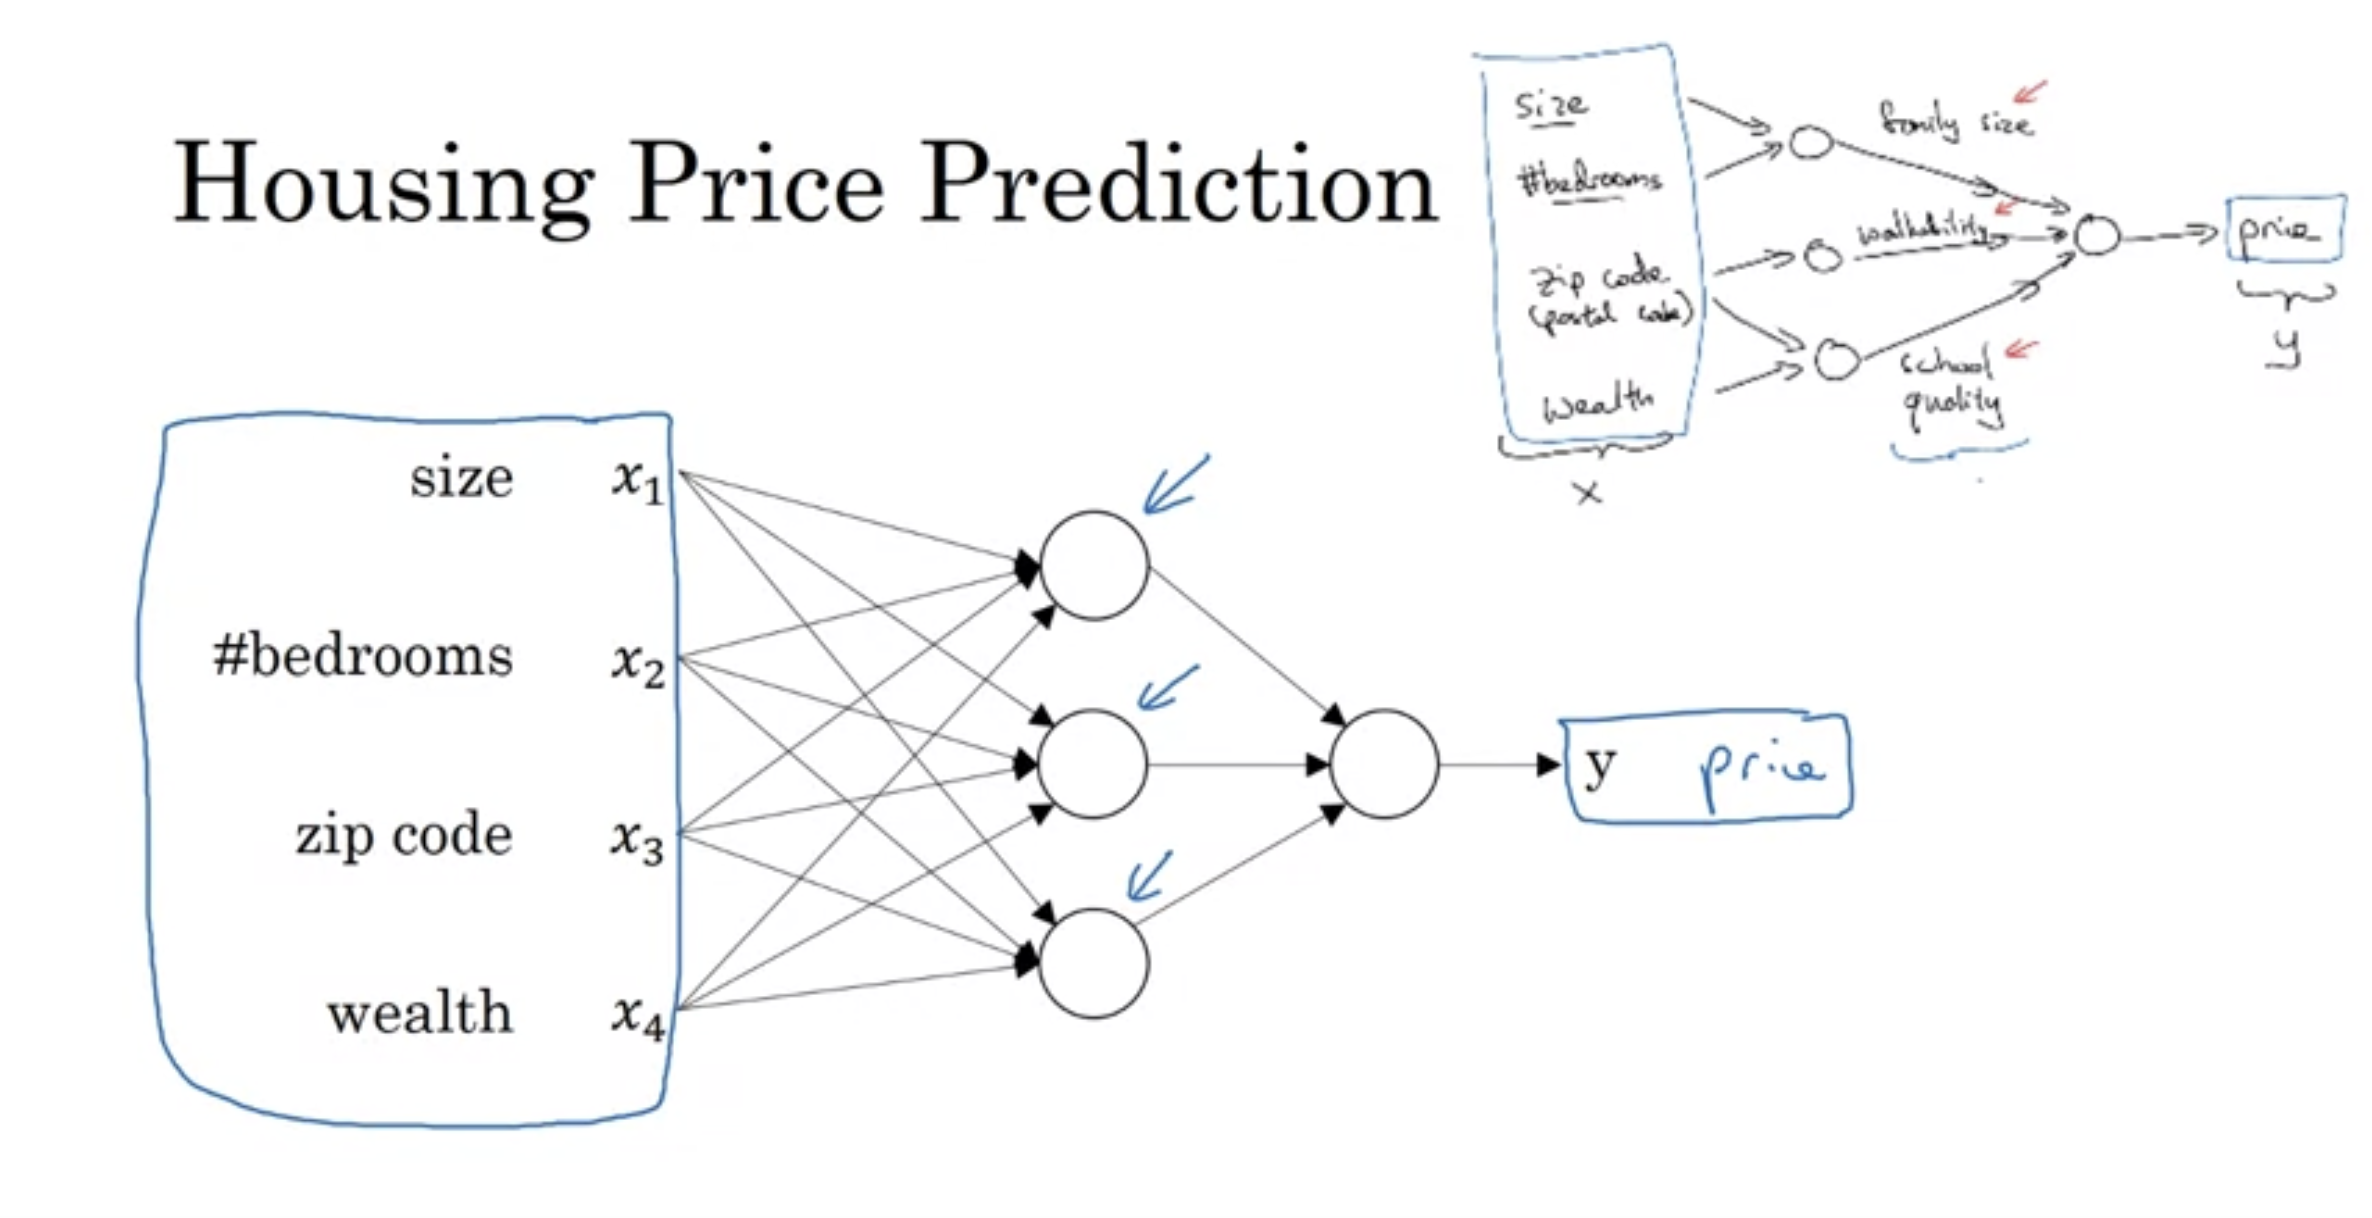
\includegraphics[width=0.75\textwidth]{Images/Simple Neural Network.png}
	\caption{A Simple Neural Network for House Price Prediction}
	\label{fig:1}
\end{figure}
\FloatBarrier

% ------------------ Supervised Learning with Neural Networks -----------------------------%
\subsection{Supervised Learning with Neural Networks}
Neural networks have gained a lot of attention lately for their ability to solve complex problems effectively. In supervised learning, you input data and aim to predict an output. Examples include predicting house prices or online ad clicks. Neural networks have been successful in various applications, like online advertising, computer vision, speech recognition, and machine translation. Different types of neural networks are used based on the nature of the data, such as convolutional neural networks for images and recurrent neural networks for sequential data. Structured data, like database entries, and unstructured data, like images or text, are both now interpretable by neural networks, thanks to recent advancements. While neural networks are often associated with recognizing images or text, they also excel in processing structured data, leading to improved advertising and recommendation systems. The techniques covered in this course apply to both structured and unstructured data, reflecting the versatility of neural networks in various applications.

\begin{figure}[h]
	\centering
	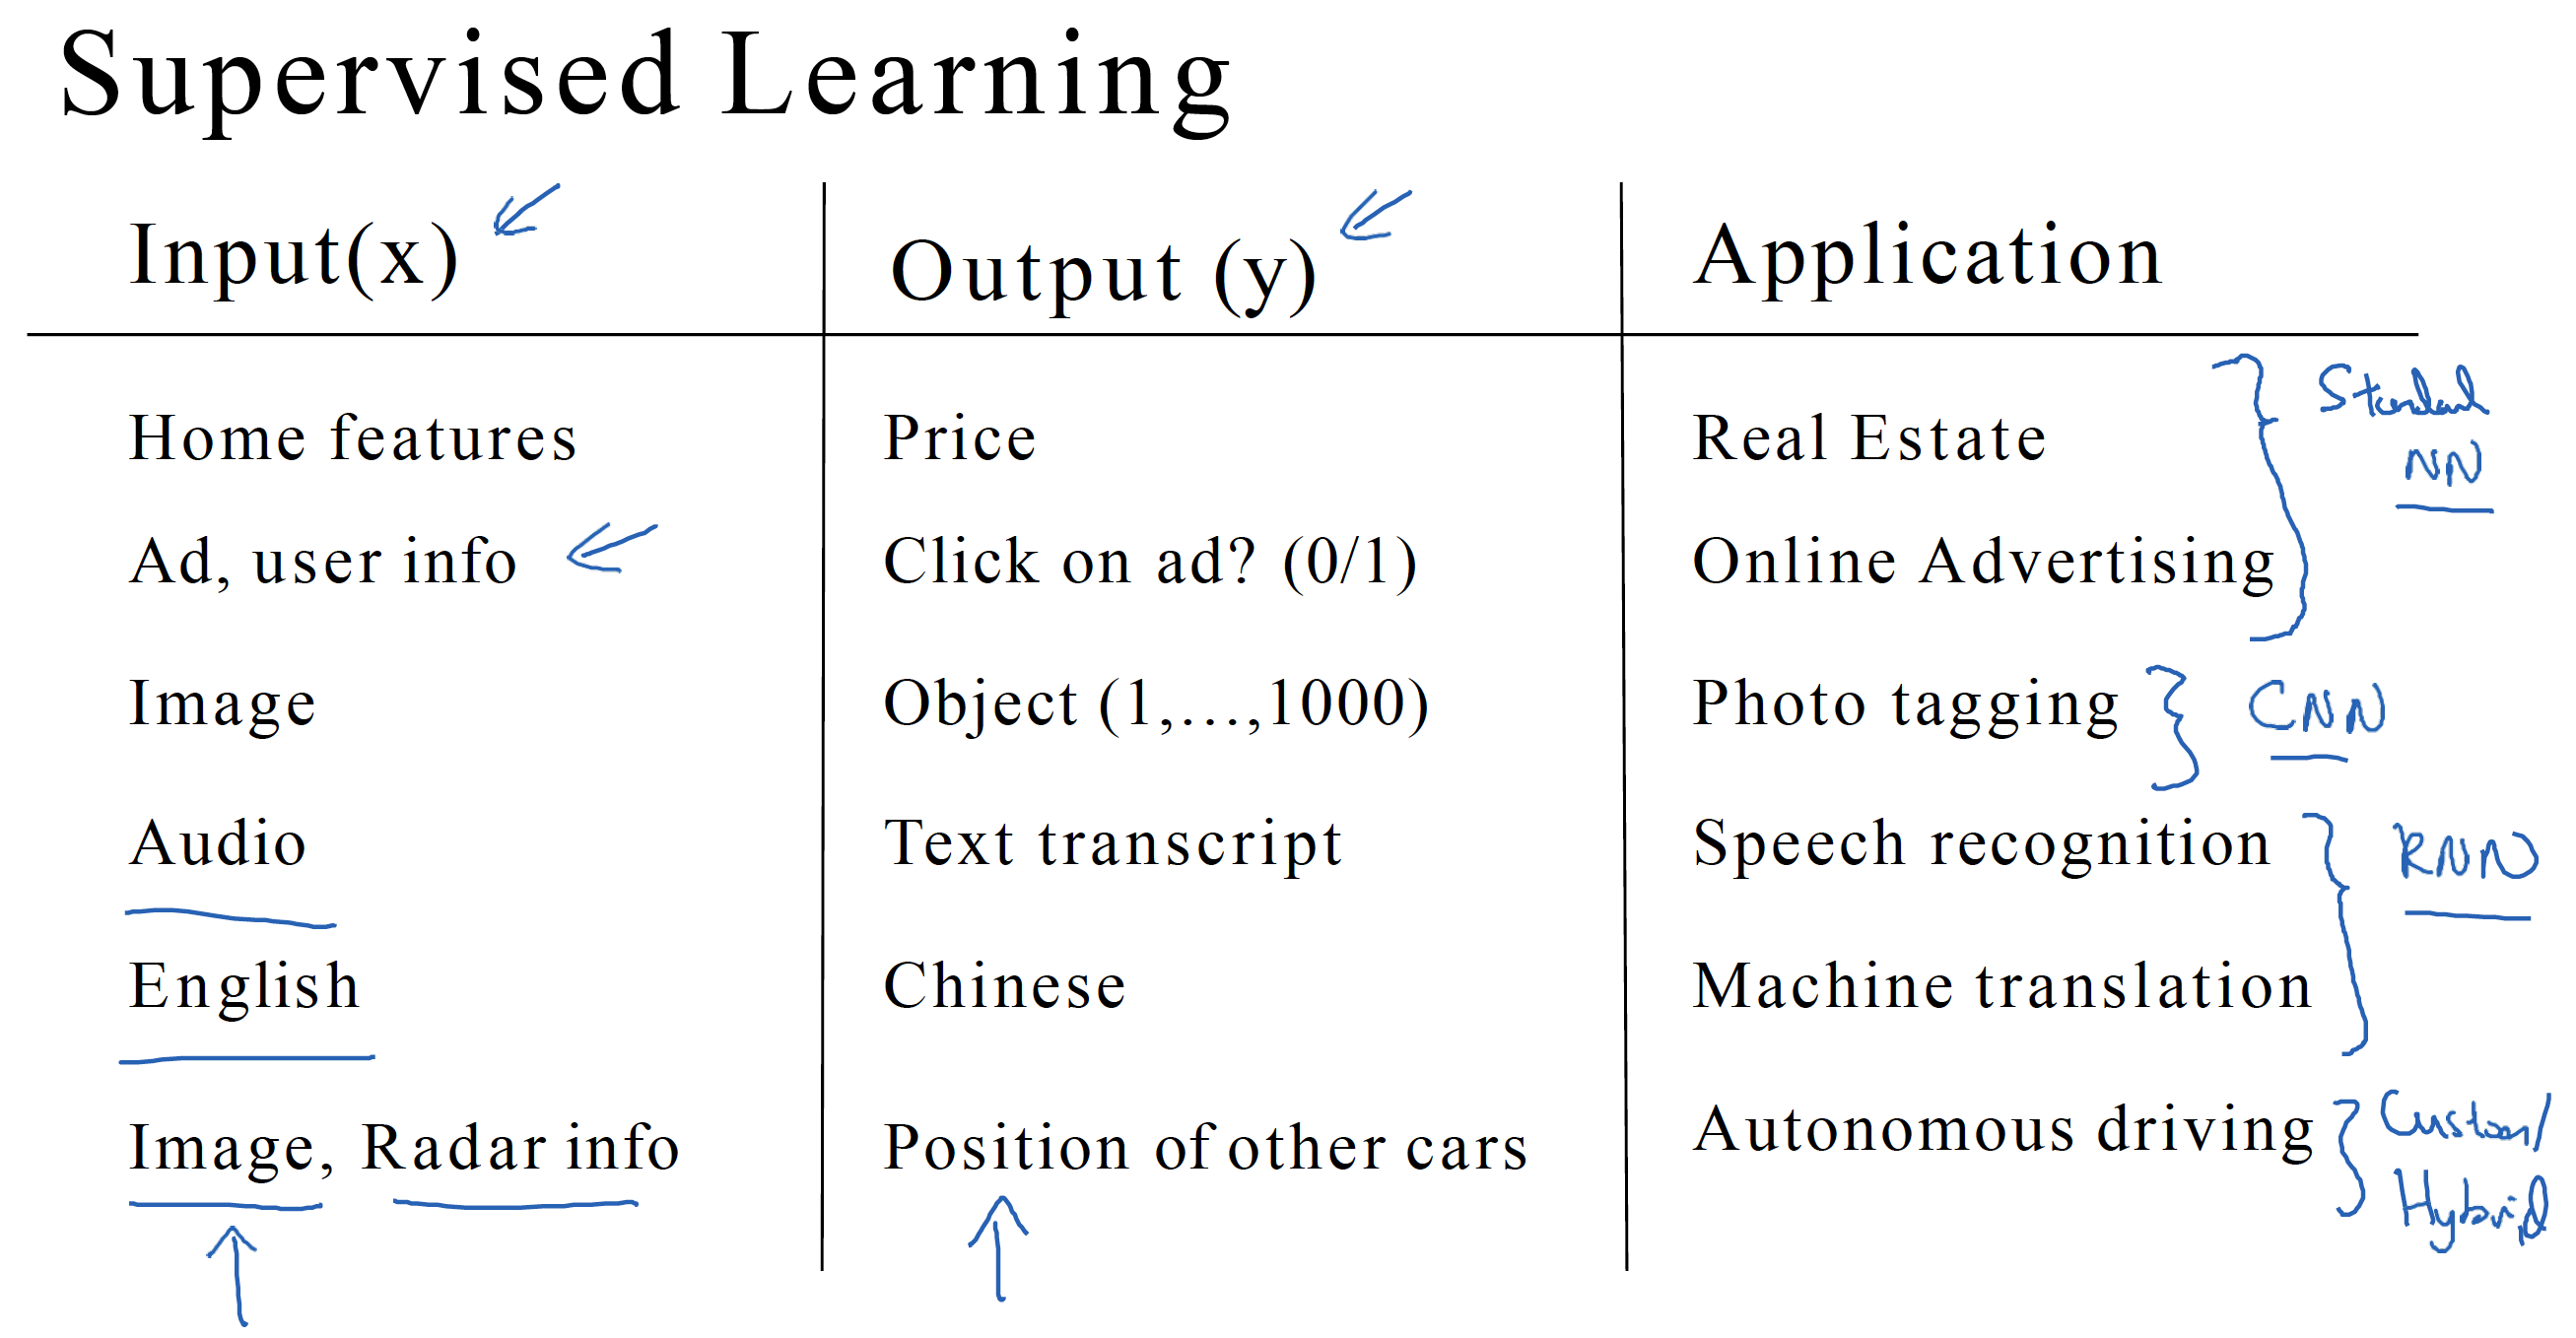
\includegraphics[width=0.75\textwidth]{Images/Supervised learning.png}
	\caption{Examples of Supervised learning}
	\label{fig:2}
\end{figure}

\begin{figure}[h]
	\centering
	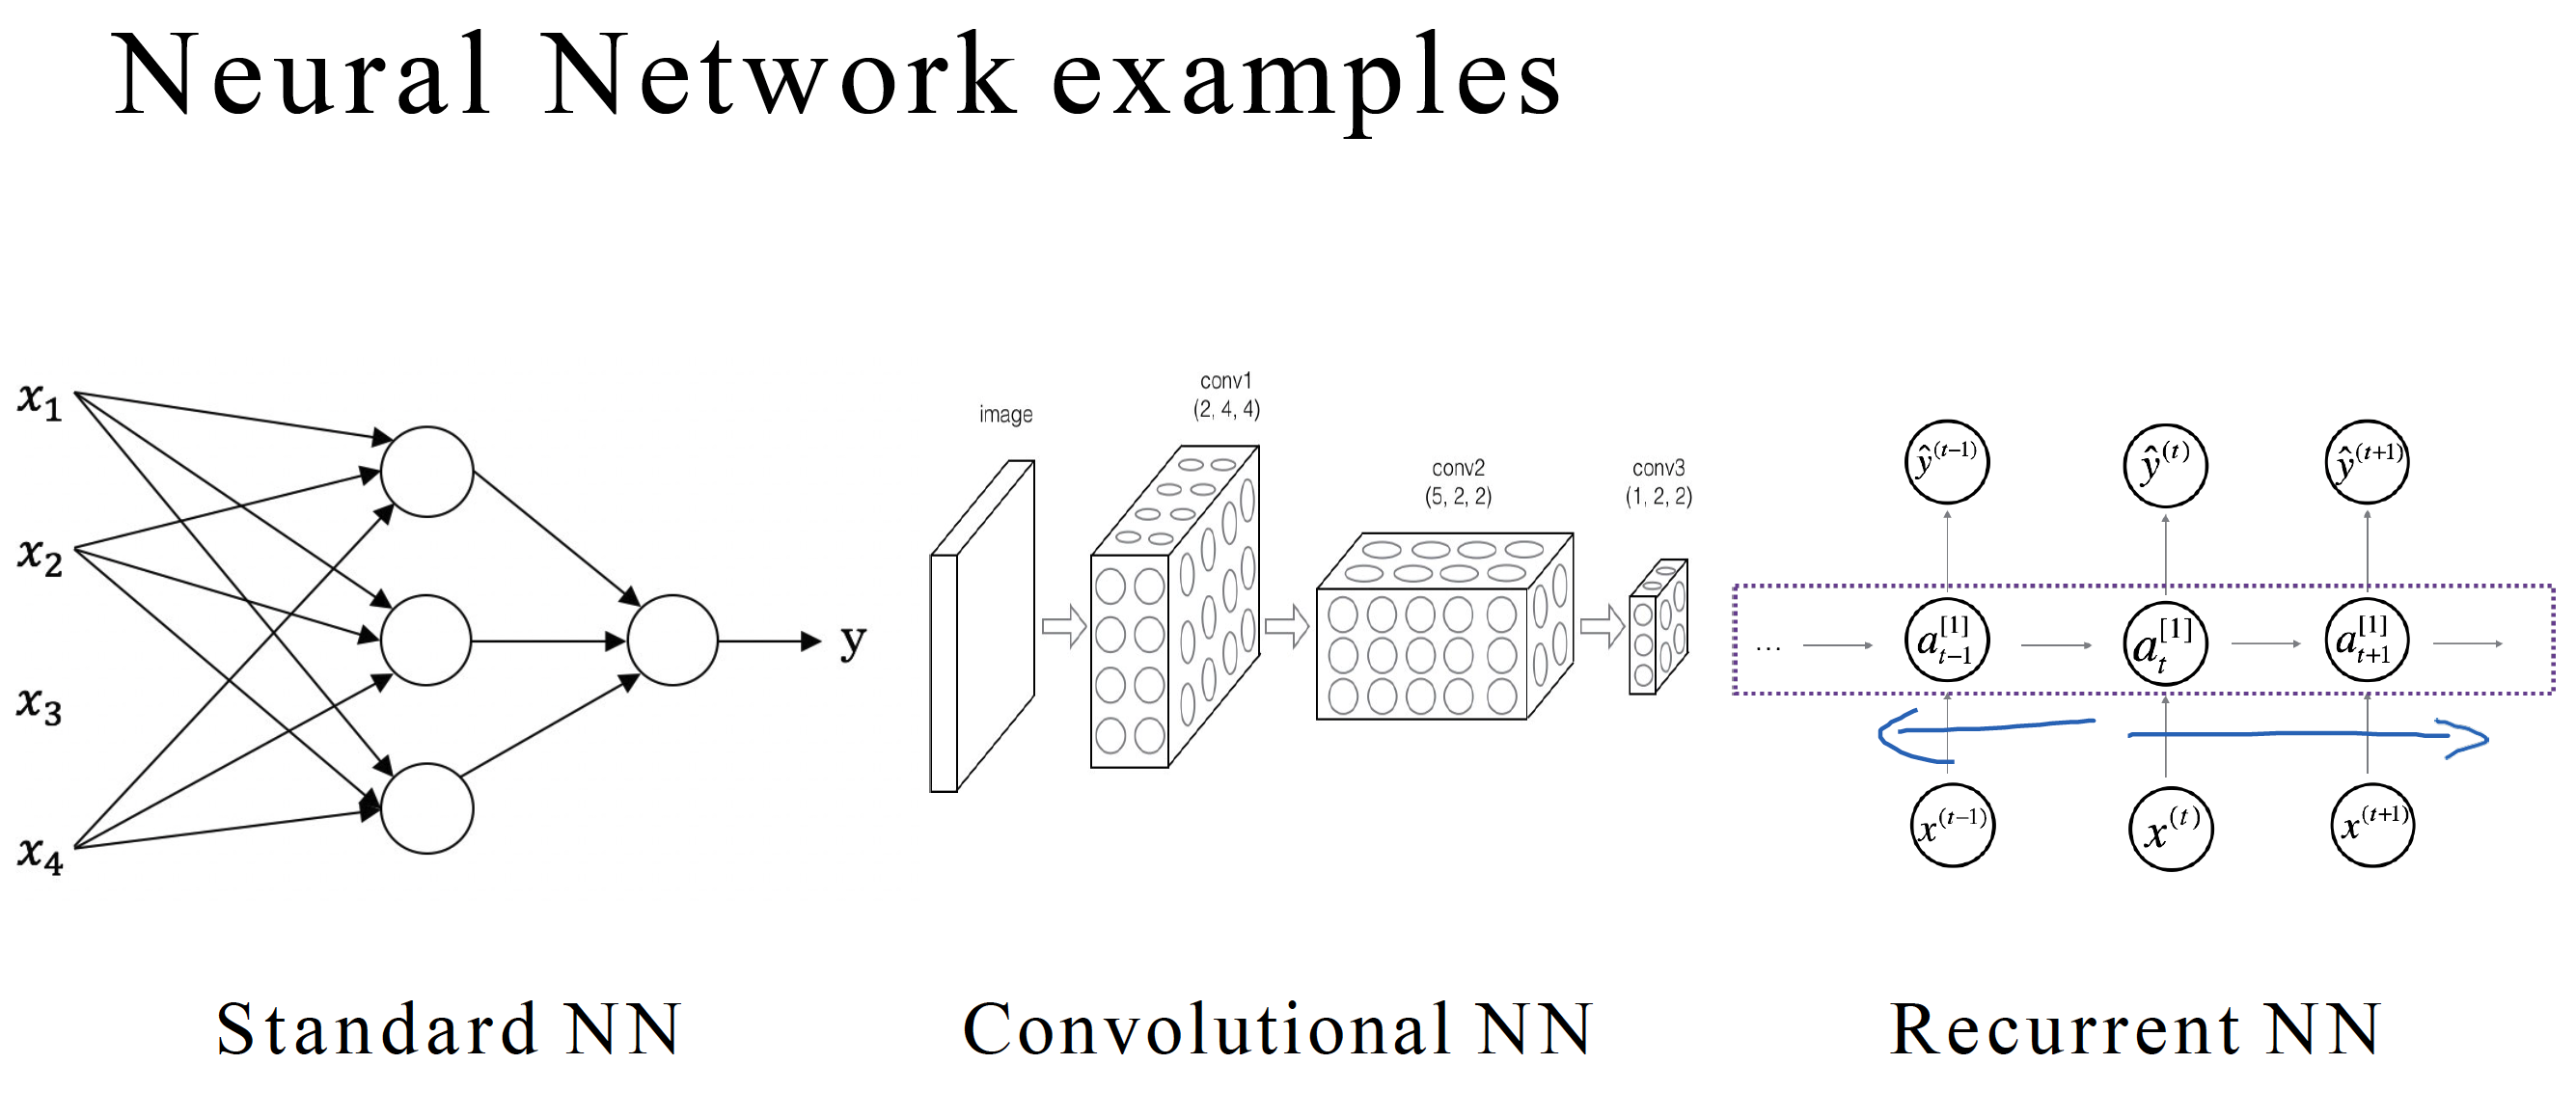
\includegraphics[width=0.75\textwidth]{Images/Neural network examples.png}
	\caption{Neural network examples}
	\label{fig:3}
\end{figure}
\FloatBarrier

\subsection{Why is Deep Learning taking off?}
The rise of deep learning has been fueled by several key factors. One major driver is the abundance of data available for training machine learning models. With the digitization of society, activities performed on digital devices generate vast amounts of data, enabling neural networks to learn from large datasets. Additionally, advancements in hardware, such as GPUs and specialized processors, have facilitated the training of large neural networks by providing faster computation speeds. Algorithmic innovations, like the adoption of the ReLU activation function, have also played a crucial role in accelerating learning processes. By reducing the time required to train models and enabling faster experimentation, these innovations have enhanced productivity and fostered rapid progress in deep learning research. Moving forward, the continued growth of digital data, advancements in hardware technology, and ongoing algorithmic research are expected to further drive improvements in deep learning capabilities. As a result, deep learning is poised to continue evolving and delivering advancements in various applications for years to come.

\begin{funfact}[frametitle=\facttitlep{FunFact}{What's drives Deep Learning}]
Deep Learning took off in the last few years and not before mainly because of great computing power and huge amount of data. These two are the key components for the successes of deep learning. The performance of a neural network improves with more training data.
\end{funfact}

\begin{figure}[h]
	\centering
	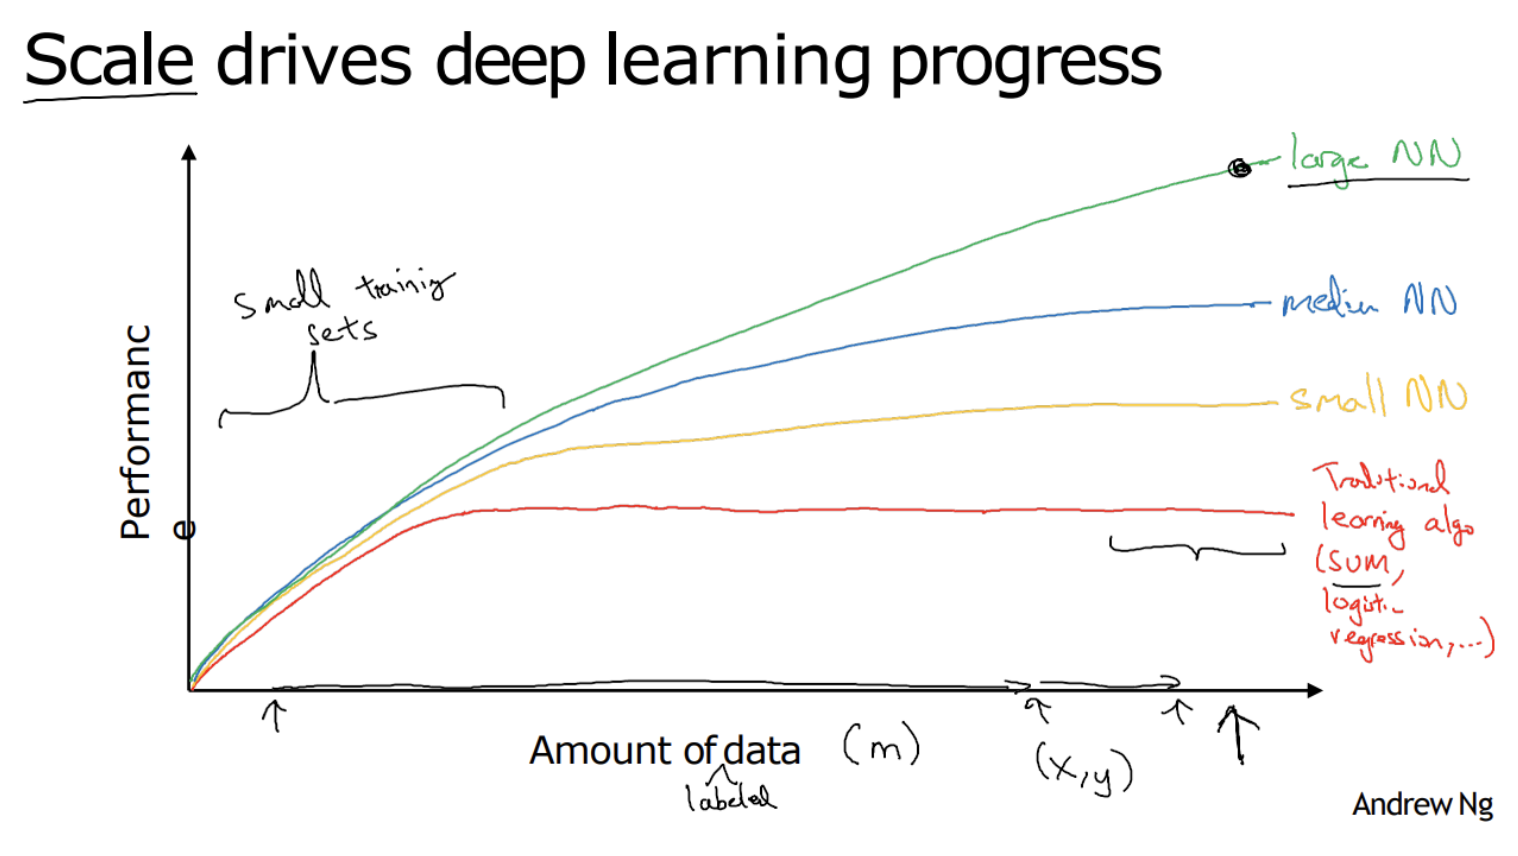
\includegraphics[width=0.75\textwidth]{Images/Scale and neural network.png}
	\caption{Scale drives neural networks}
	\label{fig:4}
\end{figure}
\FloatBarrier

% ------------------ Neural Network Basics -----------------------------%
\section{Neural Network Basics}
% ------------------ Logistic Regression as a Neural Network -----------------------------%
\subsection{Logistic Regression as a Neural Network}
Logistic regression is an algorithm for binary classification problem.  In a binary classification problem,  the goal is to train a classifier for which the input is an image represented by a feature vector, $x$, and predicts whether the corresponding label $y$ is 1 or 0. In this case, whether this is a cat image (1) or a non-cat image (0). 

\begin{figure}[h]
	\centering
	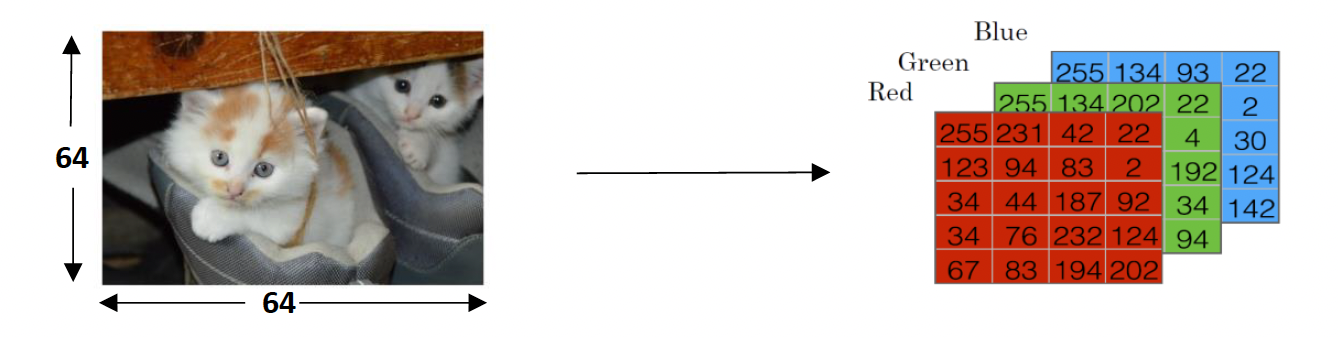
\includegraphics[width=0.95\textwidth]{Images/Binary classification cat example.png}
	\caption{Binary classification - Cat vs Non-Cat}
	\label{fig:5}
\end{figure}
\FloatBarrier

An image is stored in the computer in three separate matrices corresponding to the Red, Green, and Blue color channels of the image. The three matrices have the same size as the image, for example, the resolution of the cat image is 64 pixels x 64 pixels, the three matrices (RGB) are 64 x 64 each. The value in a cell represents the pixel intensity which will be used to create a feature vector of $n$ dimension. In pattern recognition and machine learning, a feature vector represents an image, Then the classifier's job is to determine whether it contain a picture of a cat or not.
To create a feature vector, $x$, the pixel intensity values will be ``unrolled'' or ``reshaped'' for each color. The dimension of the input feature vector $x$ is $n = 64* 64* 3 = 12288$. Hence, we use $n_x = 12288$ to represent the dimensions of the feature vectors. 

\begin{example}
     In binary classification, our goal is to learn a classifier that can input an image represented by this feature vector $x$ and predict whether the corresponding label $y$ is 1 or 0, that is, whether this is a cat image or a non-cat image. 
\end{example}

\begin{figure}[h]
	\centering
	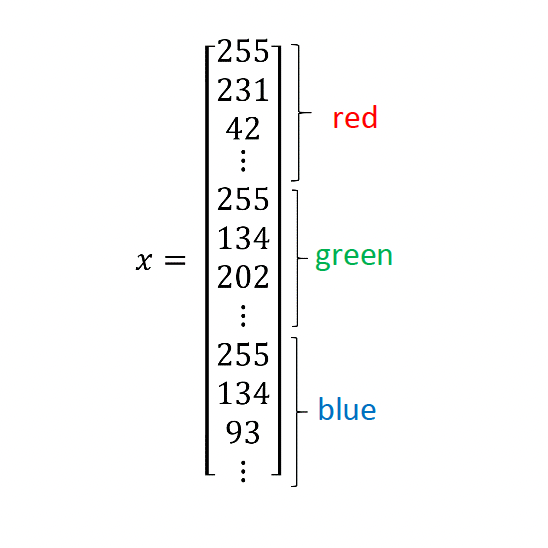
\includegraphics[width=0.35\textwidth]{Images/Reshaped feature vector.png}
	\caption{Reshaped feature vector}
	\label{fig:6}
\end{figure}
\FloatBarrier

% ------------------ Logistic Regression -----------------------------%
\subsection*{Logistic Regression}
In Logistic regression, the goal is to minimize the error between the prediction and the training data. Given an image represented by a feature vector $x$, the algorithm will evaluate the probability of a cat being in that image.

\begin{equation}
\text{Given}~ x , \hat{y} = P(y=1|x), \text{where}~0 \leq \hat{y} \leq 1
\end{equation}
The parameters used in Logistic regression are:
\begin{itemize}[nosep]
\item The input features vector: $x \in \mathbb{R}^{n_x}$, where $n_x$ is the number of features
\item The training label: $y \in 0,1$
\item The weights: $w \in \mathbb{R}^{n_x}$, where $n_x$ is the number of features
\item The threshold: $b \in \mathbb{R}$
\item The output: $\hat{y} = \sigma*(w^T*x+b)$
\item Sigmoid function: $s = \sigma(w^T*x+b) = \sigma(z)= \frac{1}{1+e^{-z}}$
\end{itemize}
$w^Tx+b$ is a linear function $(ax+b)$, but since we are looking for a probability constraint between $[0,1]$, the sigmoid function is used. The function is bounded between $[0,1]$ as shown in the graph above.
Some observations from the graph:
\begin{enumerate}[nosep]
\item If $z$ is a large positive number, then $\sigma(z) = 1$
\item If $z$ is small or large negative number, then $\sigma(z) = 0$
\item If $z=0$, then $\sigma(z) = 0.5$
\end{enumerate}

\begin{example}
     The difference between the cost function and the loss function for logistic regression is that the loss function computes the error for a single training example while the cost function is the average of the loss functions of the entire training set. 
\end{example}

Logistic regression makes use of the sigmoid function which outputs a probability between 0 and 1. The sigmoid function with some weight parameter $\theta$ or $w$ and some input $x^{(i)}$ is defined as follows. 

\begin{figure}[h]
	\centering
	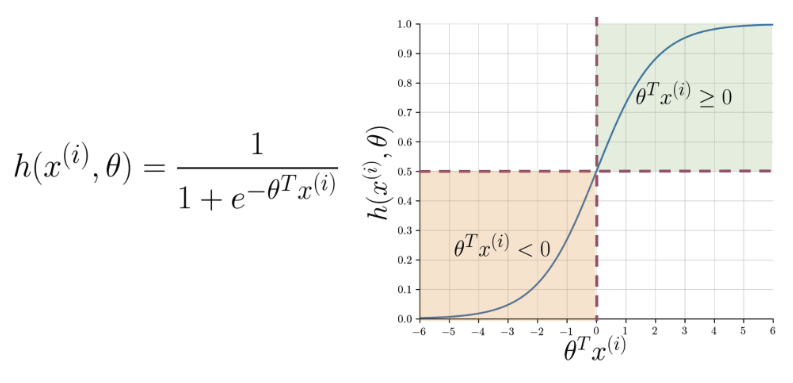
\includegraphics[width=0.85\textwidth]{Images/Logistic with sigmoid fxn.png}
	\caption{Logistic Regression Overview}
	\label{fig:7}
\end{figure}

Note that as $\theta^T x^{(i)}$ i.e.  $w^Tx$ gets closer and closer to $-\infty$ the denominator of the sigmoid function gets larger and larger and as a result, the sigmoid gets closer to 0.  On the other hand, as $\theta^T x^{(i)}$ i.e.  $w^Tx$ gets closer and closer to $\infty$ the denominator of the sigmoid function gets closer to 1 and as a result the sigmoid also gets closer to 1. 

\begin{example}
    When we implement logistic regression,  our job is to try to learn parameters $w$ and $b$ so that $\hat{y}$ becomes a good estimate of the chance of $y$ being equal to one. 
\end{example}

% ------------------ Logistic Regression Cost Function -----------------------------%
\subsection*{Logistic Regression Cost Function}
The \emph{loss function} ($\mathcal{L}$) is a function we need to define to measure how good our output $\hat{y}$ is when the true label is $y$. The loss function measures how well we are doing on a single training example. \\
\textcolor{RoyalBlue}{$\text{Loss function}~ \Rightarrow~ \mathcal{L}(\hat{y}, y) = - y*log~\hat{y} + (1 - y)*log(1 - \hat{y})$}

The \emph{cost function} ($\mathcal{J}$), which measures how we are doing on the entire training set. So the cost function, which is applied to your parameters $w$ and $b$, is going to be the average, really one of the $m$ of the sum of the loss function apply to each of the training examples.  \\
\textcolor{RoyalBlue}{$\text{Cost function}~  \Rightarrow~ \mathcal{J}(w, b) = \frac{1}{m} \sum_{i=1}^m \mathcal{L}(\hat{y}, y) = - \frac{1}{m}  \sum_{i=1}^m[y^{(i)}*log~\hat{y}^{(i)} + (1 - y^{(i)})*log(1 - \hat{y}^{(i)})]$}

\begin{figure}[h]
	\centering
	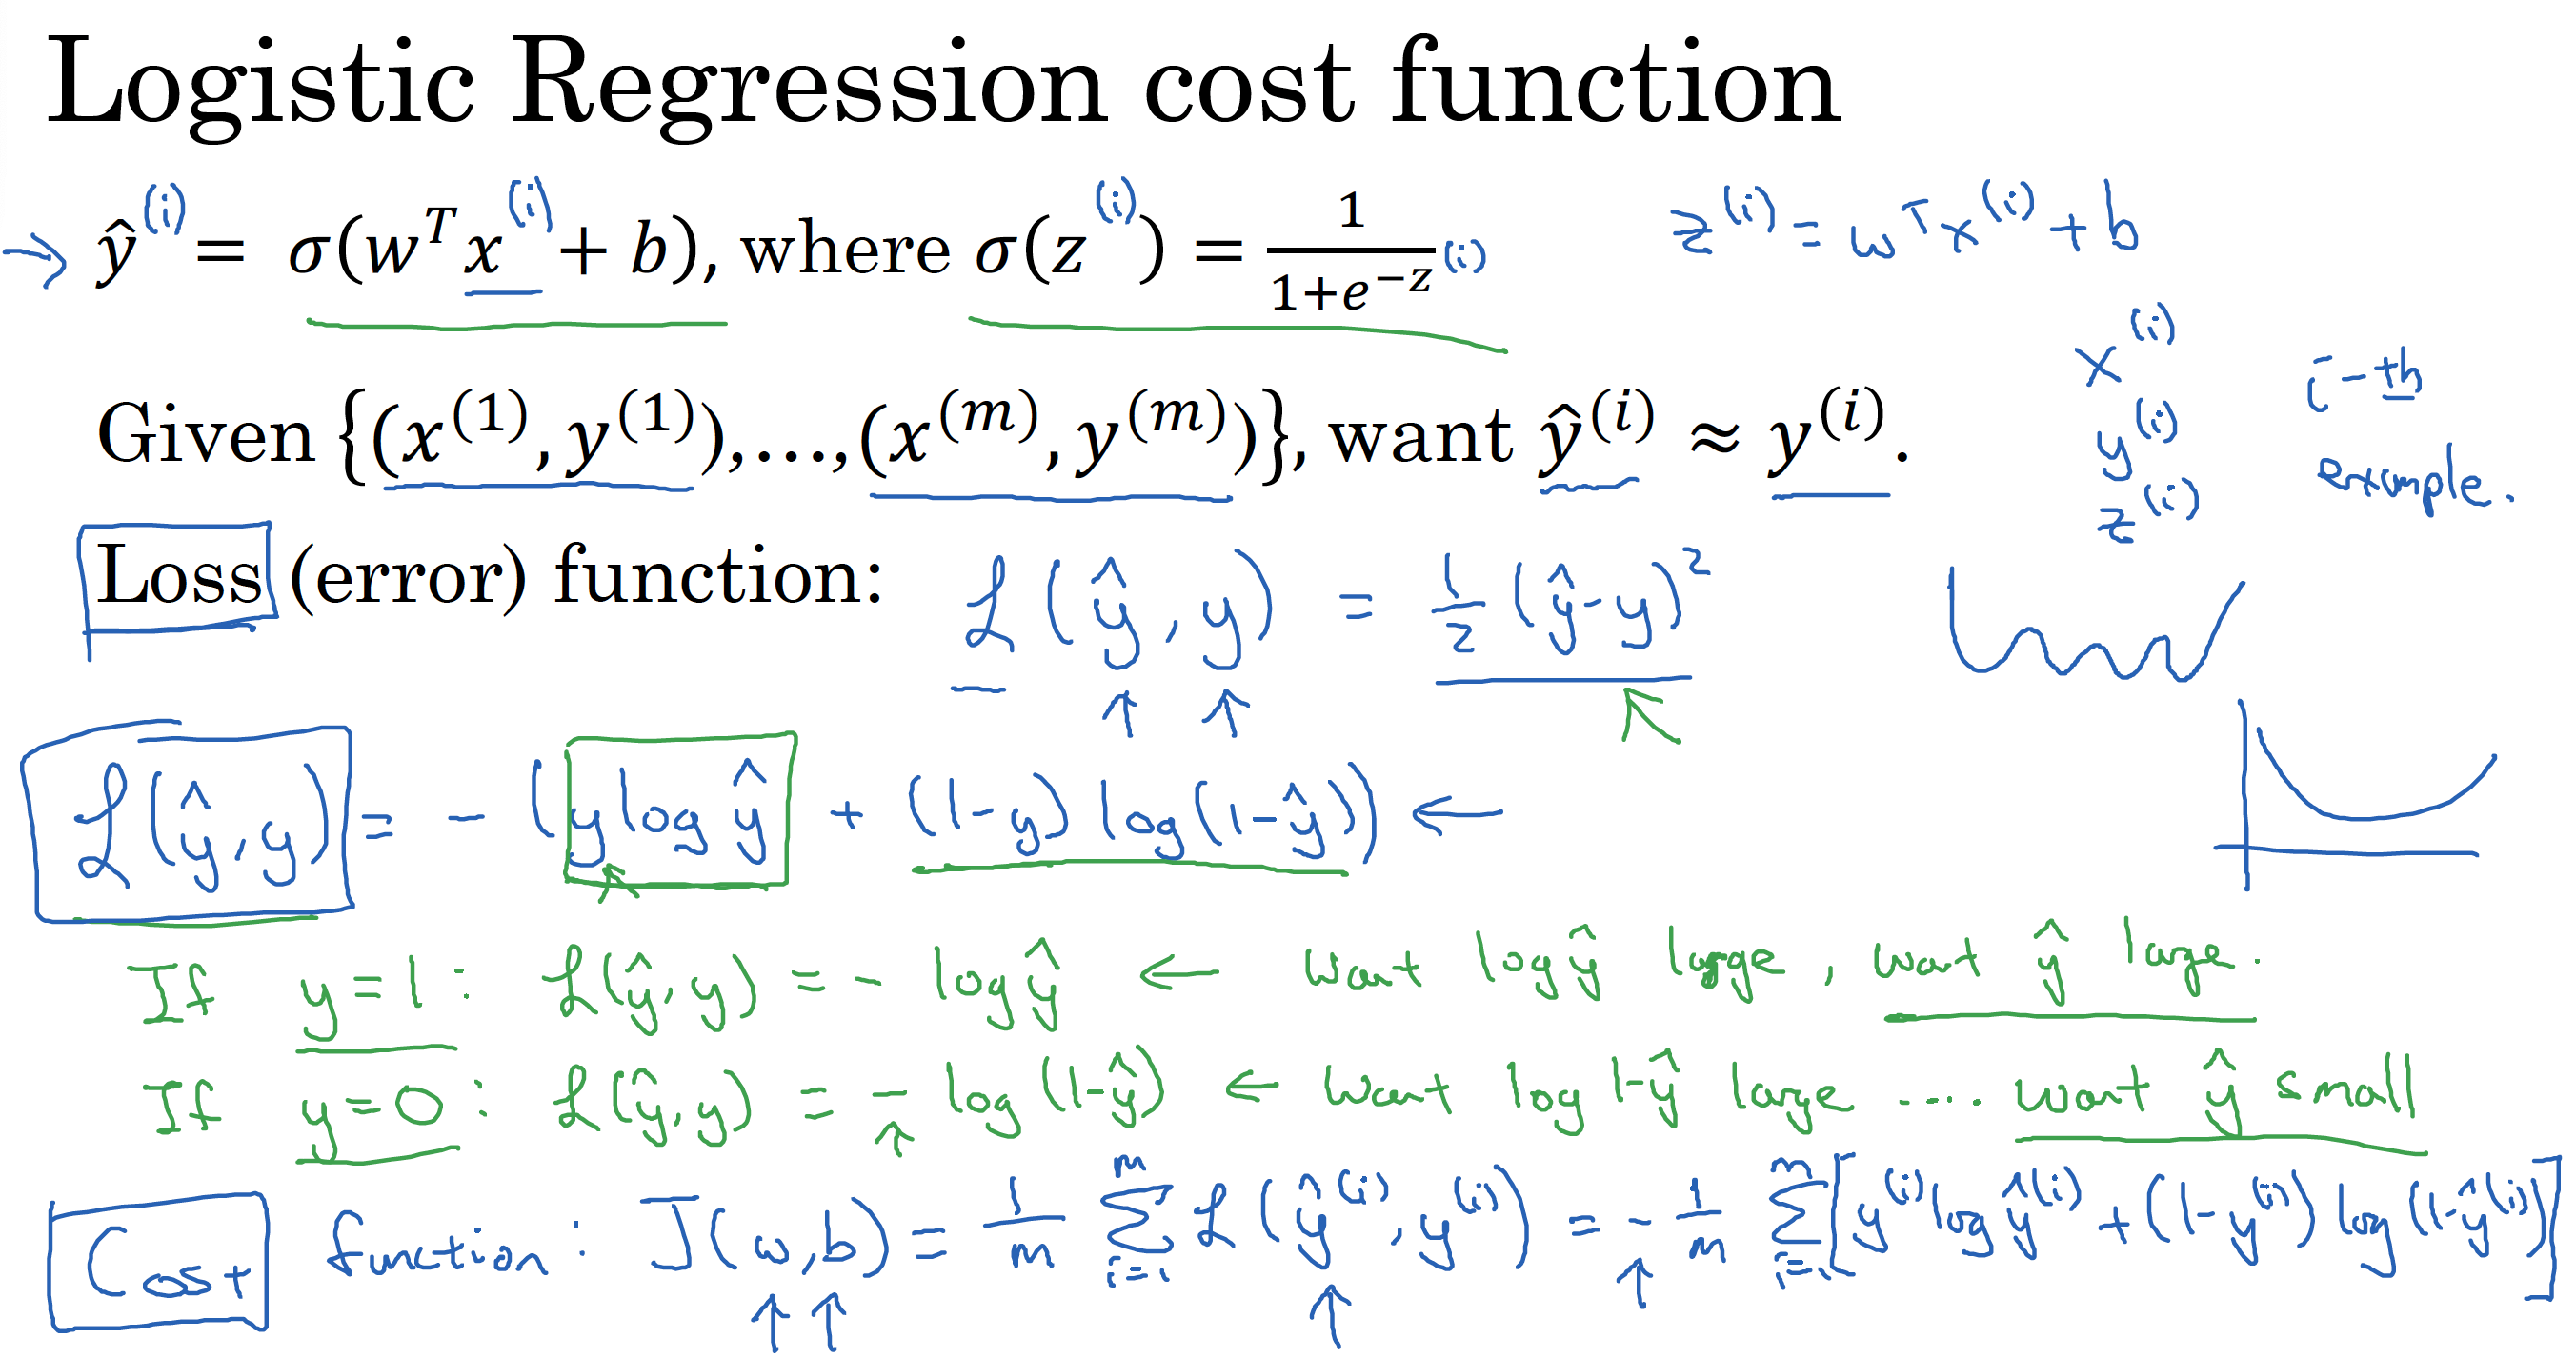
\includegraphics[width=0.85\textwidth]{Images/Cost function.png}
	\caption{Logistic Regression Cost function}
	\label{fig:8}
\end{figure}
\FloatBarrier

\begin{figure}[h]
	\centering
	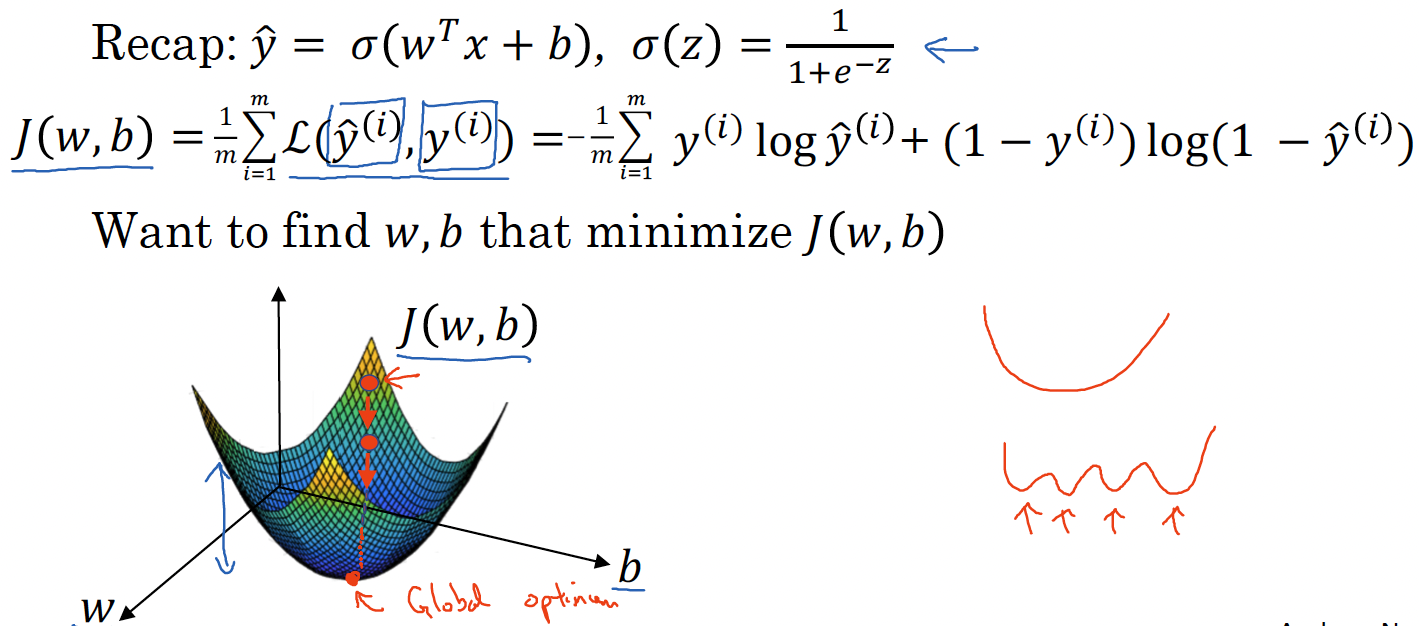
\includegraphics[width=0.85\textwidth]{Images/Gradient descent plot.png}
	\caption{Gradient Descent}
	\label{fig:9}
\end{figure}
\FloatBarrier

In logistic regression, you use the cost function $\mathcal{J}(w, b)$ to measure how well your parameters perform on the entire training set. The goal is to minimize $ \mathcal{J}(w, b)$ using gradient descent, which iteratively updates the parameters by moving in the direction of steepest descent. Because the cost function is convex, gradient descent will converge to the global minimum, regardless of initialization.

\begin{figure}[h]
	\centering
	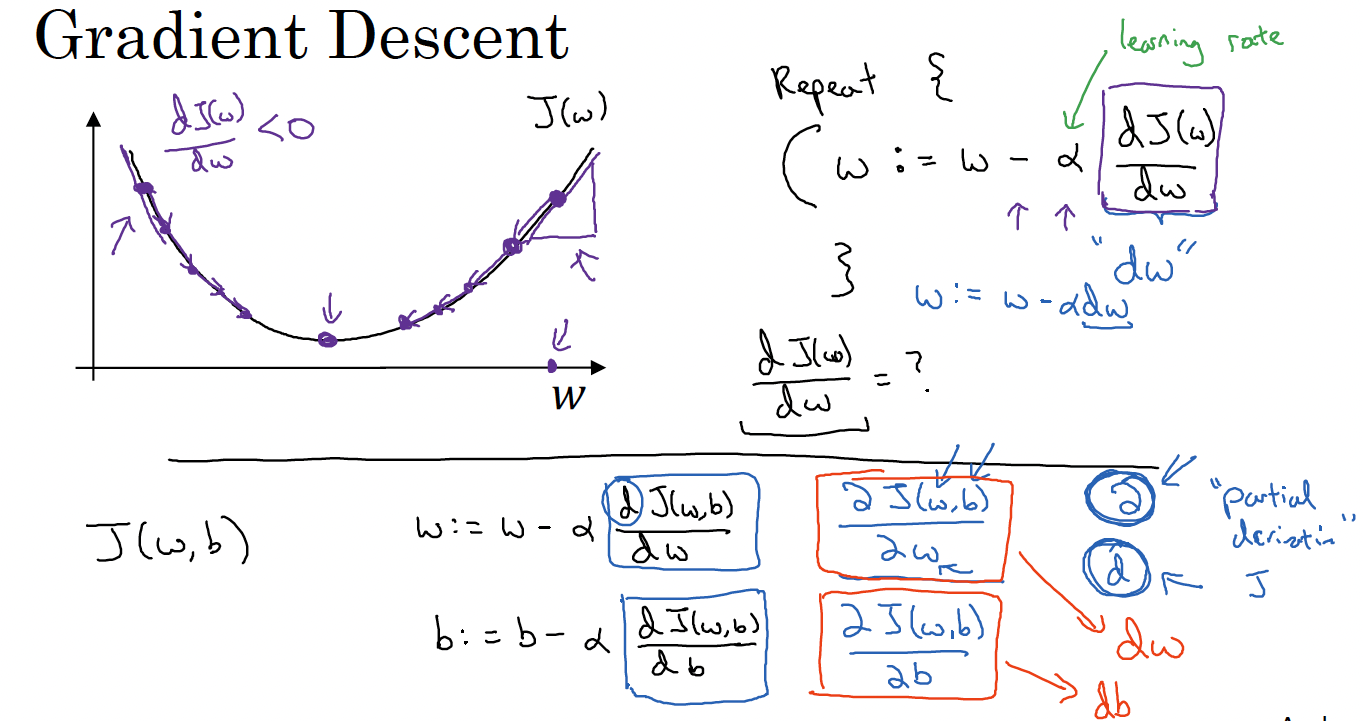
\includegraphics[width=0.75\textwidth]{Images/Gradient descent.png}
	\caption{Gradient descent Optimization}
	\label{fig:10}
\end{figure}
\FloatBarrier

% ------------------ Gradient Descent -----------------------------%
\subsection{Gradient Descent}
\begin{funfact}
Imagine you're on top of a big hill where the goal is to get to the lowest point.
Here's how you would do it:

\begin{itemize}[nosep]
\item Look around you to see which way the ground slopes down the most. 
\item Take a step in that direction. 
\item Now that you're in a new spot, look around again to see which way is downhill.
\item Take another step in that direction. 
\item Keep doing this over and over: look for the downhill direction, then take a step. 
\item Eventually, you'll reach a point where there's no more downhill to go. You're at the bottom!
\end{itemize}

This is basically what gradient descent does. The ``hill'' is like a mathematical function we're trying to minimize. ``Looking around'' is like calculating the gradient (which tells us which direction is downhill).``Taking a step'' is like updating our parameters (our position on the hill). We keep doing this until we can't go any lower (we've reached the minimum of the function).

The trick is to not take steps that are too big (or you might overshoot the bottom) or too small (or it will take forever to get there). In the algorithm, we control this with something called the ``learning rate''. That's gradient descent! It's a way of finding the lowest point by always moving downhill, little by little.
\end{funfact}

\textbf{Gradient descent} is an optimization technique used to minimize a function, often applied in machine learning for model training. The algorithm starts with an initial guess for the parameters and iteratively updates them by moving in the direction of the negative gradient (the direction of steepest descent) of the function, until it reaches a local minimum. The step size, or learning rate, controls how big each move is.

The gradient descent update rule is:

\[
\theta_{\text{new}} = \theta_{\text{old}} - \alpha \nabla J(\theta)
\]
where:
\begin{itemize}
    \item \( \theta \) are the parameters we want to optimize.
    \item \( \alpha \) is the learning rate (step size).
    \item \( \nabla J(\theta) \) is the gradient of the cost function \( J(\theta) \) with respect to \( \theta \).
\end{itemize}
This rule ensures that we move in the direction of the steepest descent, reducing the value of \( J(\theta) \) with each iteration.

\subsubsection{Why It Works}
The gradient of a function points in the direction of the steepest ascent. By moving in the opposite direction of the gradient, the function value decreases, eventually reaching a local or global minimum. As the gradient approaches zero, the parameter values converge toward the minimum.

\subsubsection{Pseudocode}
Below is the pseudocode for gradient descent in simple terms:

\begin{lstlisting}
initialize $\theta$ (e.g., random values) 
choose learning rate $\alpha$
repeat until convergence:
    $\quad$ compute gradient $\nabla J(\theta)$
    $\quad$ update $\theta: \theta = \theta - \alpha * \nabla J(\theta)$
\end{lstlisting}

\begin{algorithm}
\caption{Gradient Descent}
\begin{flushleft}
\textbf{Input:} Initial parameter $\theta^0$, gradient of loss function $\nabla J(\theta)$, learning rate $\alpha$, tolerance $\epsilon$, maximum iterations $max\_iter$\\
\textbf{Output:} Optimized parameter $\theta$\\

$iter \leftarrow 0$\\
\textbf{while} $iter < max\_iter$ \textbf{do}\\
\hspace{1em}Compute $\nabla J(\theta)$\\
\hspace{1em}\textbf{if} $\|\nabla J(\theta)\| < \epsilon$ \textbf{then}\\
\hspace{2em}\textbf{break}\\
\hspace{1em}\textbf{end if}\\
\hspace{1em}$\theta \leftarrow \theta - \alpha \nabla J(\theta)$\\
\hspace{1em}$iter \leftarrow iter + 1$\\
\textbf{end while}\\
\textbf{return} $\theta$
\end{flushleft}
\end{algorithm}

The process repeats until the gradient is close to zero, indicating the function has been minimized.

\begin{example}
Gradient descent is an optimization algorithm used to minimize the cost function of a model by iteratively adjusting the model's parameters. The goal is to find the values of the parameters (like weights in a machine learning model) that minimize the cost function, which measures how well the model fits the data.
\end{example}

\subsubsection*{How Gradient Descent Works:}
\begin{enumerate}
    \item \textbf{Initialize Parameters:} Start with an initial guess for the parameters (e.g., weights). This can be a set of random values or zeros.
    
    \item \textbf{Calculate the Gradient:} Compute the gradient (i.e., the partial derivative) of the cost function with respect to each parameter. The gradient indicates the direction of the steepest increase in the cost function.
    
    \item \textbf{Update the Parameters:} Adjust the parameters in the opposite direction of the gradient (i.e., the direction that reduces the cost function). The size of the step taken is controlled by a learning rate, a hyperparameter that determines how big the steps are.
    
    \[
    \text{new parameter} = \text{current parameter} - \text{learning rate} \times \text{gradient}
    \]
    
    \item \textbf{Repeat:} Continue recalculating the gradient and updating the parameters until the algorithm converges, meaning the changes in the cost function become very small, indicating that a minimum has been reached.
\end{enumerate}

\newpage
\begin{funfact}[frametitle=\facttitlep{FunFact}{Computation Graph}]
The computation graph organizes a computation from left-to-right computation. Through a left-to-right pass, we can compute the value of $\mathcal{J}$. In order to compute derivatives there'll be a right-to-left pass, kind of going in the opposite direction called backwards propagation. That would be most natural for computing the derivatives. 
\end{funfact}

\textbf{Forward Propagation}: Computes the output $y$ from the input $X$ by passing through the network layers. \\
\textbf{Backward propagation} adjusts the network's parameters (weights and biases) by propagating the error backward from the output to the input, using the gradients to minimize the loss.

% ------------------ Shallow Neural Networks -----------------------------%
\section{Shallow Neural Networks}
% ------------------ Neural Network Representation -----------------------------%
\subsection{Neural Network Representation}
A neural network is a machine learning model inspired by the human brain. It consists of layers of interconnected nodes (neurons) where each connection has a weight, representing its importance. Neural networks process input data by passing it through these layers, applying activation functions to transform the data, and adjusting the weights based on the output error during training. The goal is to minimize the error and improve the model's predictions. Neural networks are widely used in tasks like image recognition, language processing, and complex data modeling.

\begin{figure}[h]
	\centering
	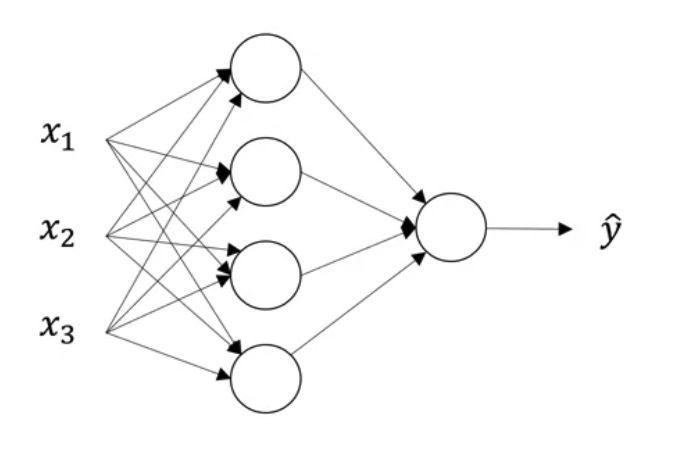
\includegraphics[width=0.65\textwidth]{Images/Shallow Neural Network.png}
	\caption{Shallow Neural Network}
	\label{fig:11}
\end{figure}

% ------------------ Neural Network Structure -----------------------------%
\subsection{Neural Network Structure}
A simple neural network has similar structure as a linear classifier:
\begin{itemize}[nosep]
\item A neuron takes inputs from other neurons (-> input into linear classifier)
\item The inputs are summed in a weighted manner (-> weighted sum)
	\begin{itemize}[label={\ding{224}}]
		\item Learning is through a modification of the weights (gradient descent in the case of NN)
	\end{itemize}
\item If it receives enough inputs, it “fires” (if it exceeds the threshold or weighted sum plus bias is high enough)
\item The output of a neuron can be modulated by a non linear function (e.g sigmoid).
\end{itemize}

\begin{figure}[h]
	\centering
	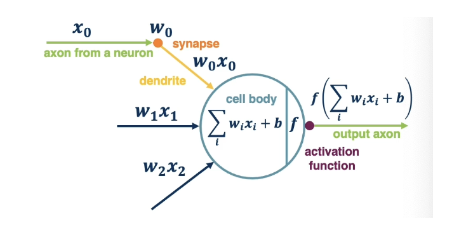
\includegraphics[width=0.65\textwidth]{Images/Activation function.png}
	\caption{Structure of a simple neural network}
	\label{fig:12}
\end{figure}

A neural network consists of three primary layers: input, hidden, and output layers as shown in \textbf{Fig. \ref{fig:13}}.

\begin{figure}[h]
	\centering
	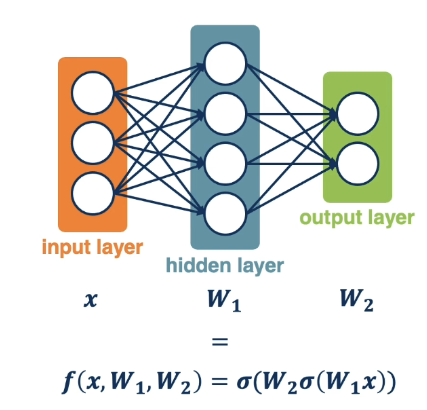
\includegraphics[width=0.5\textwidth]{Images/Layers in a neural network.png}
	\caption{Layers in a neural network}
	\label{fig:13}
\end{figure}

\begin{figure}[h]
	\centering
	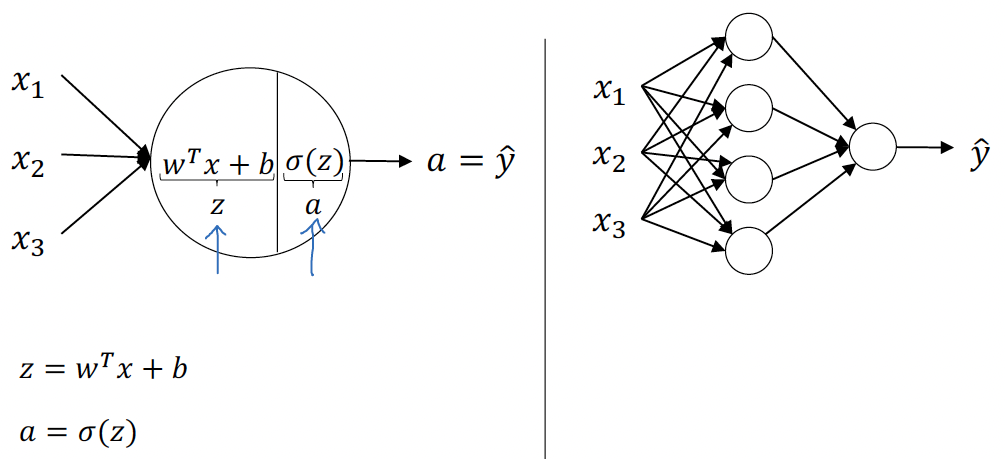
\includegraphics[width=0.85\textwidth]{Images/Neural Network Representation.png}
	\caption{Neural Network Representation}
	\label{fig:14}
\end{figure}
\FloatBarrier

\subsubsection{Input Layer}
The \textbf{input layer} is responsible for taking in the features of the data. For example, features \( x_1, x_2, x_3 \) are passed into the network in \textbf{Fig. \ref{fig:14}}, and these values are referred to as the \textit{activations} of the input layer, denoted \( A^{[0]} \).

\subsubsection{Hidden Layer}
The \textbf{hidden layer} processes the input features. It is called \textit{hidden} because, during training, the true values for these nodes are not seen in the training data. The activations of this layer are denoted \( A^{[1]} \), where each node \( A^{[1]}_i \) represents an activation value computed using a weight matrix \( W^{[1]} \) and bias vector \( b^{[1]} \). For example, if there are four hidden units, \( A^{[1]} \) will be a 4-dimensional vector.

\subsubsection{Output Layer}
The \textbf{output layer} produces the final prediction \( \hat{y} \), based on the activations from the hidden layer. The output is represented as \( A^{[2]} \), a single scalar value in this example.

\subsubsection{Notation}
We use the following notations to represent the activations in different layers:
\begin{itemize}
    \item \( A^{[0]} \): Activations of the input layer.
    \item \( A^{[1]} \): Activations of the hidden layer.
    \item \( A^{[2]} \): Output, representing \( \hat{y} \).
\end{itemize}

In the neural network in \textbf{Fig. \ref{fig:14}}, each layer has associated weight matrices and biases:
\begin{itemize}
    \item \( W^{[1]} \) is a \( 4 \times 3 \) matrix (4 hidden units, 3 input features).
    \item \( b^{[1]} \) is a \( 4 \times 1 \) vector (for 4 hidden units).
    \item \( W^{[2]} \) is a \( 1 \times 4 \) matrix (1 output unit, 4 hidden units).
    \item \( b^{[2]} \) is a \( 1 \times 1 \) scalar (for the output unit).
\end{itemize}

While this neural network has three layers (input, hidden, output), it is commonly referred to as a \textbf{two-layer network} because the input layer is not counted. Therefore, the hidden layer is called \textit{layer 1} and the output layer \textit{layer 2}.

\subsubsection{Training}
The parameters \( W \) and \( b \) are optimized during training to minimize the error between the predicted output \( \hat{y} \) and the actual output \( y \). In this process, the neural network learns the best weights and biases for making accurate predictions.

% ------------------ Activation Functions -----------------------------%
\subsection{Activation Functions}
Activation functions are mathematical equations that determine the output of a neural network node. They introduce non-linearity into the model, enabling the network to learn complex patterns. Below are some common activation functions used in neural networks:

\subsubsection{1. Sigmoid Function}
The \textbf{sigmoid} activation function is defined as:
\[
a = \sigma(x) = \frac{1}{1 + e^{-z}}
\]
It compresses input values to a range between 0 and 1, making it useful for models that need probabilities as output or binary classification. However, it suffers from the \textit{vanishing gradient problem}, where gradients become very small, slowing down learning.

\subsubsection{2. Tanh Function}
The \textbf{tanh} activation function is defined as:
\[
a = \text{tanh}(z) = \frac{e^{z} - e^{-z}}{e^{z} + e^{-z}}
\]
It outputs values between -1 and 1, centered around zero, making learning more efficient in some cases. Like sigmoid, it also suffers from vanishing gradients but it is superior to the sigmoid function for hidden layers.

\subsubsection{3. ReLU (Rectified Linear Unit)}
The \textbf{ReLU} activation function is defined as:
\[
a = \text{ReLU}(z) = \max(0, z)
\]
ReLU is simple and efficient, especially in deep networks, because it allows faster convergence. The downside is that it can cause ``dead neurons'' (neurons that output 0 for all inputs), which may stop learning in certain neurons.

\subsubsection{4. Leaky ReLU}
The \textbf{Leaky ReLU} activation function is defined as:
\[
a = \max(0.01z, z)
\]
The Leaky ReLU adresses the ReLU's zero-gradient issue by allowing small negative values. Generally works better than ReLU but is used less frequently.

\subsubsection{5. Softmax Function}
The \textbf{softmax} function is commonly used in the output layer for classification tasks. It converts raw outputs (logits) into probabilities:
\[
\text{Softmax}(z_i) = \frac{e^{z_i}}{\sum_{j}e^{z_j}}
\]
This is useful for multi-class classification, ensuring the sum of output probabilities equals 1.

\subsubsection{Choosing an Activation Function}
\textbf{ReLU} is popular for hidden layers in deep neural networks due to its simplicity and efficiency.  \textbf{Sigmoid} and \textbf{tanh} are useful in smaller networks or specific scenarios but less common in modern deep networks.  \textbf{Softmax} is used in the output layer for multi-class classification tasks.
\begin{itemize}
    \item \textbf{Output Layer}: Use \textbf{Sigmoid} for binary classification.
    \item \textbf{Hidden layers}: \textbf{ReLU} is the default choice, though \textbf{tanh} can also be used effectively.
    \item \textbf{Learning Efficiency}: \textbf{ReLU} and \textbf{Leaky ReLU} often result in faster learning compared to sigmoid or tanh, as their gradients do not saturate easily.
\end{itemize}

Each activation function has its specific use cases depending on the task and network architecture.

\begin{figure}[h]
	\centering
	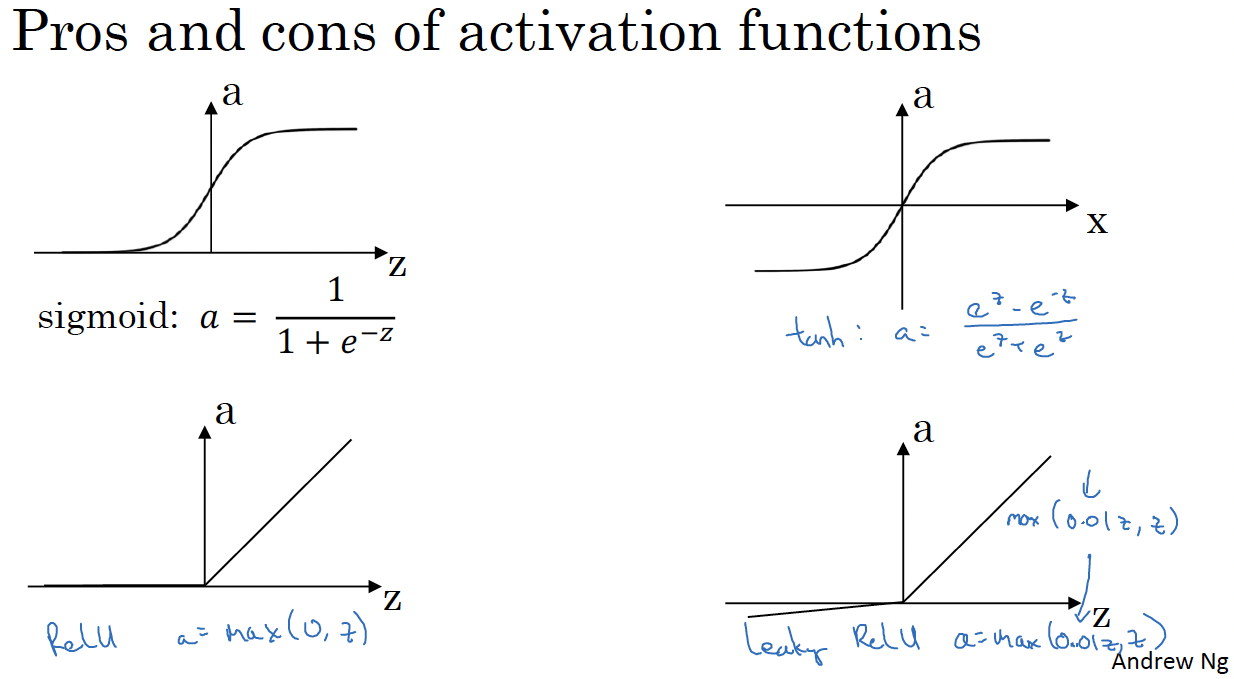
\includegraphics[width=0.75\textwidth]{Images/Activation functions.png}
	\caption{Activation Functions in Neural Networks}
	\label{fig:15}
\end{figure}
\FloatBarrier

% ------------------ Deep Neural Networks ---------------------------%
\section{Deep Neural Networks}
% ------------ Deep L-layer Neural Network -----------------%
\subsection{Deep L-layer Neural Network}
A \textbf{Deep Neural Network (DNN)} is a type of artificial neural network that contains multiple layers between the input and output layers. These intermediate layers, known as \textit{hidden layers}, allow the network to learn more complex patterns and representations from the data.

\subsection*{Key Characteristics of Deep Neural Networks:}
\begin{enumerate}
    \item \textbf{Multiple Hidden Layers}:
    \begin{itemize}
        \item Unlike shallow networks (such as logistic regression or simple neural networks with a single hidden layer), a deep neural network has multiple hidden layers. The more hidden layers a network has, the ``deeper'' it is.
        \item \textit{Example}: A network with 3 hidden layers and an output layer would have a depth of 4 (input layer not counted in depth).
    \end{itemize}

    \item \textbf{Ability to Learn Complex Functions}:
    \begin{itemize}
        \item By stacking multiple layers, each layer in a DNN extracts features or patterns from the previous layer's output. This enables the network to learn complex and abstract representations of data.
        \item Shallow networks are often limited in their ability to model complex relationships, while DNNs can learn hierarchical patterns.
    \end{itemize}

    \item \textbf{Forward and Backward Propagation}:
    \begin{itemize}
        \item \textbf{Forward Propagation}: Data passes through each layer of the network, transforming via weights, biases, and activation functions, until reaching the output layer.
        \item \textbf{Backward Propagation (Backpropagation)}: The network adjusts the weights and biases by calculating errors and gradients to minimize the loss function. This allows the network to learn from the data.
    \end{itemize}

    \item \textbf{Applications}:
    \begin{itemize}
        \item DNNs are widely used in areas such as image recognition, natural language processing, speech recognition, and more.
        \item \textit{For instance}, DNNs power technologies like self-driving cars, facial recognition, and voice assistants.
    \end{itemize}

    \item \textbf{Deep vs. Shallow Networks}:
    \begin{itemize}
        \item \textbf{Shallow Network}: A neural network with one or very few hidden layers (e.g., logistic regression can be viewed as a one-layer network).
        \item \textbf{Deep Network}: A network with multiple hidden layers, enabling it to learn from more complex data.
    \end{itemize}
\end{enumerate}

\begin{example}
A deep neural network is a powerful tool for learning from data with multiple hidden layers, making it well-suited for complex tasks that require sophisticated pattern recognition. The depth of the network enables it to model intricate relationships between inputs and outputs that shallow models often cannot handle effectively.
\end{example}

\subsubsection{Notation to describe a Deep Neural Network}
\textbf{Fig. \ref{fig:16}} shows a four-layer neural network consisting of three hidden layers. The number of units in each layer of the neural network is 5, 5, 3, and 1, respectively.  
\begin{figure}[h]
	\centering
	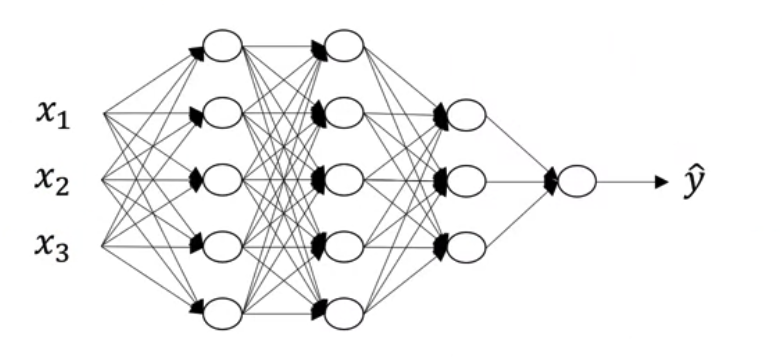
\includegraphics[width=0.75\textwidth]{Images/Deep Neural Network.png}
	\caption{Deep Neural Networks with 5 hidden layers}
	\label{fig:16}
\end{figure}
\FloatBarrier

Let: \\
\begin{itemize}
    \item \( L \): Represents the total number of layers in the network. For this network, \( L = 4 \).
    \item \( n^{[l]} \): Represents the number of units (or nodes) in layer \( l \).
    \begin{itemize}
        \item Example:
        \begin{itemize}
            \item \( n^{[0]} = n_x = 3 \) (input layer).
            \item \( n^{[1]} = 5 \), \( n^{[2]} = 5 \), \( n^{[3]} = 3 \) (hidden layers).
            \item \( n^{[4]} = n^{[L]} = 1 \) (output layer).
        \end{itemize}
    \end{itemize}
    \item \( a^{[l]} \): Denotes the activations of layer \( l \).
    \begin{itemize}
        \item \( a^{[0]} = x \): Activations in the input layer, equivalent to the input features.
        \item \( a^{[L]} = \hat{y} \): Activations in the final layer, equivalent to the predicted output.
    \end{itemize}
    \item \( W^{[l]} \): Denotes the weights for computing \( z^{[l]} \) in layer \( l \).
    \item \( b^{[l]} \): Denotes the biases for computing \( z^{[l]} \) in layer \( l \).
\end{itemize}

\subsubsection*{Activation Functions}
In forward propagation, the activation in layer \( l \), \( a^{[l]} \), is computed as:
\[
a^{[l]} = g(z^{[l]}),
\]
where \( g \) is the activation function, and \( z^{[l]} \) depends on \( W^{[l]} \) and \( b^{[l]} \).

\subsubsection*{Summary of Relationships}
\begin{itemize}
    \item The input layer (\( l = 0 \)): \( a^{[0]} = x \).
    \item The output layer (\( l = L \)): \( a^{[L]} = \hat{y} \) (the network's prediction).
    \item Each layer computes \( z^{[l]} \) using weights (\( W^{[l]} \)) and biases (\( b^{[l]} \)).
\end{itemize}

% ------------ Forward propagation in Deep Neural Network -----------------%
\subsection{Forward propagation in a Deep Neural Network}
Forward propagation in a deep neural network involves passing the input data through the network, layer by layer, to compute the output prediction. Below are the steps to carry out forward propagation:

\newpage
\subsection*{Steps for Forward Propagation}

\begin{enumerate}
    \item \textbf{Input Layer Initialization}:
    \begin{itemize}
        \item Denote the input features as \( x \).
        \item The activations of the input layer are \( a^{[0]} = x \).
    \end{itemize}

    \item \textbf{Layer-wise Computation}: 
	\begin{itemize}
		\item For each layer \( l \) from \( 1 \) to \( L \) (the total number of layers):
		\begin{enumerate}
	        \item \textbf{Linear Combination}: Compute the pre-activation \( z^{[l]} \):
	        \[
	        z^{[l]} = W^{[l]} a^{[l-1]} + b^{[l]},
	        \]
	        where:
	        \begin{itemize}
	            \item \( W^{[l]} \) is the weight matrix for layer \( l \),
	            \item \( b^{[l]} \) is the bias vector for layer \( l \),
	            \item \( a^{[l-1]} \) are the activations from the previous layer.
	        \end{itemize}
	
	        \item \textbf{Activation Function}: Apply an activation function \( g^{[l]} \) to \( z^{[l]} \) to compute the activations \( a^{[l]} \):
	        \[
	        a^{[l]} = g^{[l]}(z^{[l]}).
	        \]
	        The activation function could be ReLU, sigmoid, tanh, or softmax, depending on the task and the layer type.
	   	 \end{enumerate}
	\end{itemize}
    
    \item \textbf{Output Layer}:
    \begin{itemize}
        \item At the final layer \( L \), compute the prediction:
        \[
        a^{[L]} = \hat{y}.
        \]
        \item If it's a regression problem, \( \hat{y} \) is a continuous value (e.g., no activation or linear activation).
        \item For classification, \( \hat{y} \) might involve a sigmoid or softmax activation.
    \end{itemize}
\end{enumerate}

\subsubsection*{Algorithm}

Given \( x \) as input, perform the following:
\begin{itemize}
    \item Initialize \( a^{[0]} = x \).
    \item For \( l = 1 \) to \( L \):
    \begin{itemize}
        \item Compute \( z^{[l]} = W^{[l]} a^{[l-1]} + b^{[l]} \).
        \item Compute \( a^{[l]} = g^{[l]}(z^{[l]}) \).
    \end{itemize}
    \item Return \( a^{[L]} = \hat{y} \), the final prediction.
\end{itemize}

\subsubsection*{Example}

Consider a network with:
\begin{itemize}
    \item Input: \( x \) (dimension: \( n_x \)),
    \item Hidden layers: two layers with ReLU activation,
    \item Output layer: one node with sigmoid activation.
\end{itemize}

Forward propagation involves:
\begin{enumerate}
    \item Compute \( z^{[1]} = W^{[1]} x + b^{[1]} \), \( a^{[1]} = \text{ReLU}(z^{[1]}) \),
    \item Compute \( z^{[2]} = W^{[2]} a^{[1]} + b^{[2]} \), \( a^{[2]} = \text{ReLU}(z^{[2]}) \),
    \item Compute \( z^{[3]} = W^{[3]} a^{[2]} + b^{[3]} \), \( \hat{y} = \text{sigmoid}(z^{[3]}) \).
\end{enumerate}

\subsubsection*{Matrix Dimensions}

\begin{itemize}
    \item \( W^{[l]} \): Dimensions \( [n^{[l]}, n^{[l-1]}] \),
    \item \( b^{[l]} \): Dimensions \( [n^{[l]}, 1] \),
    \item \( z^{[l]} \): Dimensions \( [n^{[l]}, m] \), where \( m \) is the number of training examples,
    \item \( a^{[l]} \): Same as \( z^{[l]} \).
\end{itemize}

\subsubsection*{Advantages of Forward Propagation}
\begin{itemize}
    \item Enables computation of the network's output given any input.
    \item Forms the basis for backward propagation, which updates weights and biases during training.
\end{itemize}

% ------------ Vectorization Method in Deep Neural Network -----------------%
\subsection{Understanding Vectorization Method in Deep Neural Networks}

In the previous discussion, we described what constitutes a deep \( L \)-layer neural network and introduced the notation to represent such networks. This note elaborates on performing forward propagation in a deep network, first for a single training example \( x \), and later for the entire training set using vectorization.

\subsection*{Forward Propagation for a Single Training Example}

\begin{enumerate}
    \item \textbf{Layer 1 Computation}:
    \begin{itemize}
        \item Compute \( z^{[1]} = W^{[1]} x + b^{[1]} \), where \( W^{[1]} \) and \( b^{[1]} \) are the parameters of the first layer.
        \item The activations for the first layer are \( a^{[1]} = g^{[1]}(z^{[1]}) \), where \( g^{[1]} \) is the activation function.
    \end{itemize}
    
    \item \textbf{Layer 2 Computation}:
    \begin{itemize}
        \item Compute \( z^{[2]} = W^{[2]} a^{[1]} + b^{[2]} \).
        \item The activations for the second layer are \( a^{[2]} = g^{[2]}(z^{[2]}) \).
    \end{itemize}
    
    \item \textbf{General Rule for Layer \( l \)}:
    \begin{itemize}
        \item Compute \( z^{[l]} = W^{[l]} a^{[l-1]} + b^{[l]} \).
        \item Compute \( a^{[l]} = g^{[l]}(z^{[l]}) \).
    \end{itemize}
    
    \item \textbf{Output Layer}:
    \begin{itemize}
        \item For the final layer \( L \), compute \( z^{[L]} = W^{[L]} a^{[L-1]} + b^{[L]} \).
        \item The predicted output is \( \hat{y} = a^{[L]} = g^{[L]}(z^{[L]}) \).
    \end{itemize}
    
    \item \textbf{Input Representation}:
    \begin{itemize}
        \item The input \( x \) is equivalent to \( a^{[0]} \), making the equations consistent across layers.
    \end{itemize}
\end{enumerate}

\subsection*{Vectorized Forward Propagation for the Entire Training Set}

To compute forward propagation for all training examples simultaneously, the equations are extended:

\begin{enumerate}
    \item \textbf{Input Layer}:
    \begin{itemize}
        \item The input matrix \( X \) represents all training examples, where each column corresponds to a training example.
        \item For layer 1:
        \[
        Z^{[1]} = W^{[1]} A^{[0]} + b^{[1]},
        \]
        where \( A^{[0]} = X \).
    \end{itemize}
    
    \item \textbf{Hidden Layers}:
    \begin{itemize}
        \item For any layer \( l \):
        \[
        Z^{[l]} = W^{[l]} A^{[l-1]} + b^{[l]},
        \]
        \[
        A^{[l]} = g^{[l]}(Z^{[l]}).
        \]
    \end{itemize}
    
    \item \textbf{Output Layer}:
    \begin{itemize}
        \item For the final layer \( L \):
        \[
        Z^{[L]} = W^{[L]} A^{[L-1]} + b^{[L]},
        \]
        \[
        A^{[L]} = \hat{Y} = g^{[L]}(Z^{[L]}).
        \]
    \end{itemize}
\end{enumerate}

\subsubsection{For Loop Implementation}

\begin{enumerate}
    \item \textbf{Forward Propagation Steps}:
    \begin{itemize}
        \item Iterate over layers \( l = 1 \) to \( L \):
        \[
        Z^{[l]} = W^{[l]} A^{[l-1]} + b^{[l]}, \quad A^{[l]} = g^{[l]}(Z^{[l]}).
        \]
    \end{itemize}
    
    \item \textbf{Explicit Loops are Acceptable}:
    \begin{itemize}
        \item Unlike some optimization steps, forward propagation necessitates an explicit loop over layers due to its sequential nature.
        \item It is perfectly valid to implement this using a loop from \( l = 1 \) to \( L \).
    \end{itemize}
\end{enumerate}

\subsubsection*{Debugging Matrix Dimensions}

A systematic approach to debugging involves verifying the matrix dimensions at each step:
\begin{itemize}
    \item \( W^{[l]} \): Shape \( [n^{[l]}, n^{[l-1]}] \).
    \item \( b^{[l]} \): Shape \( [n^{[l]}, 1] \).
    \item \( Z^{[l]} \) and \( A^{[l]} \): Shape \( [n^{[l]}, m] \), where \( m \) is the number of training examples.
\end{itemize}

This method ensures bug-free implementation and aids in understanding the flow of forward propagation in neural networks.

% ------------ Implementing Forward and Backward Propagation in Deep Neural Networks -----------------%
\subsection{Implementing Forward and Backward Propagation in Deep Neural Networks}

\subsubsection{1. Forward Propagation for layer $l$}
In forward propagation, we input \(a^{[l-1]}\) and outputs \(a^{[l]}\) and the cache \(z^{[l]}\). \\
\textbf{Purpose:} Takes input \(a^{[l-1]}\), outputs \(a^{[l]}\), and cache \(z^{[l]}\).  \\
- Cache can include \(W^{[l]}\) and \(b^{[l]}\) to simplify function calls.

\textbf{Equations:}
\[
z^{[l]} = W^{[l]} \cdot a^{[l-1]} + b^{[l]}
\]
\[
a^{[l]} = g^{[l]}(z^{[l]})
\]
where \(g\) is the activation function.

\textbf{Vectorized Implementation:}
\[
Z^{[l]} = W^{[l]} \cdot A^{[l-1]} + b^{[l]} \quad \text{(Python broadcasting for}~b^{[l]})
\]
\[
A^{[l]} = g^{[l]}(Z^{[l]}) \quad \text{(element-wise product)}
\]

\textbf{Process:}
\begin{itemize}[nosep]
\item Initialize with \(A^{[0]} = X\) (input features for one example or the entire training set).
\item Sequentially compute forward propagation for each layer from left to right.
\end{itemize}

\subsubsection{2. Backward Propagation for layer $l$}
\textbf{Purpose:} Inputs \(da^{[l]}\), outputs \(da^{[l-1]}\), \(dW^{[l]}\), and \(db^{[l]}\).

\textbf{Steps:}
\begin{align*}
dz^{[l]} &= da^{[l]} \circ g'^{[l]}(z^{[l]}) \quad \text{(element-wise product)} \\
dW^{[l]} &= dz^{[l]} \cdot a^{[l-1]^T} \\
db^{[l]} &= dz^{[l]} \\
da^{[l-1]} &= W^{[l]^T} \cdot dz^{[l]} \\
dz^{[l]} &= W^{[l+1]^T} \cdot dz^{[l+1]} \circ g'^{[l]}(z^{[l]})
\end{align*}

\textbf{Vectorized Implementation:}
\begin{align*}
dZ^{[l]} &= dA^{[l]} \circ g'^{[l]}(Z^{[l]}) \quad \text{(element-wise product)} \\
dW^{[l]} &= \frac{1}{m} dZ^{[l]} \cdot A^{[l-1]^T} \\
db^{[l]} &= \frac{1}{m} \sum dZ^{[l]} \quad \{ \text{vectorized: } \texttt{\(\frac{1}{\text{m}} \text{np.sum(dZ}^{[l]}, \text{axis}=1, \text{keepdims}=\text{True})\)} \} \\
dA^{[l-1]} &= W^{[l]^T} \cdot dZ^{[l]} \\
dZ^{[l-1]} &= W^{[l]^T} \cdot dZ^{[l]} * g'^{[l-1]}(Z^{[l-1]}) \quad \text{(element-wise multiplication)}
\end{align*}

\textbf{Initialization for Backward Propagation:} \\
To initialize backpropagation, we compute the derivative of the loss function with respect to the activation output of the final layer, \( A^{[L]} \), denoted as \( dA^{[L]} \).  \\ 
For \textbf{binary classification} using logistic regression, where the loss function is the cross-entropy loss, this initialization is given by:

\[
dA^{[L]} = - \left( \frac{Y}{A^{[L]}} - \frac{1 - Y}{1 - A^{[L]}} \right)
\]

\noindent where:
\begin{itemize}[nosep]
    \item \( Y \) is the true label (ground truth).
    \item \( A^{[L]} \) is the predicted output (\( \hat{Y} \)) from the forward propagation step.
\end{itemize}
This formula is derived by differentiating the cross-entropy loss function:
\[
\mathcal{L} = - \frac{1}{m} \sum_{i=1}^m \left( Y^{(i)} \log A^{[L](i)} + (1 - Y^{(i)}) \log (1 - A^{[L](i)}) \right)
\]
with respect to \( A^{[L]} \).

In vectorized form, for a batch of \( m \) training examples, the initialization is:
\[
dA^{[L]} = \left(- \frac{Y^{(1)}}{A^{(1)}} + \frac{1 - Y^{(1)}}{1 - A^{(1)}} - \dots - \frac{Y^{(m)}}{A^{(m)}} + \frac{1 - Y^{(m)}}{1 - A^{(m)}} \right)
\]

\subsubsection*{Key Points}
\begin{itemize}[nosep]
    \item \( dA^{[L]} \) serves as the starting gradient for the backward pass.
    \item Once \( dA^{[L]} \) is initialized, it is propagated backward through the layers to compute the gradients of the weights (\( dW^{[l]} \)), biases (\( db^{[l]} \)), and previous layer activations (\( dA^{[l-1]} \)).
\end{itemize}

\subsubsection*{Summary of Forward and Backward Pass}
\textbf{Forward Propagation:}
\begin{itemize}[nosep]
\item Input \(X\), pass through layers (e.g., ReLU, Sigmoid for binary classification).
\item Outputs \(\hat{y}\) for loss computation.
\end{itemize}

\textbf{Backward Propagation:}
\begin{itemize}[nosep]
 \item Compute derivatives \(dW^{[l]}\), \(db^{[l]}\), and propagate \(dA^{[l]}\) backward using caches (\(z^{[l]}\), \(a^{[l]}\)).
 \item Discard \(dA^{[0]}\) as it’s not needed.
\end{itemize}

% ----------- Understanding Hyperparameters in Deep Neural Networks ---------------%
\subsection{Understanding Hyperparameters in Deep Neural Networks}

Being effective in developing your deep neural networks requires that you not only organize your parameters well but also your hyperparameters. 

\subsubsection*{What Are Hyperparameters?}
The parameters of your model are \( W \) and \( b \) .i.e.,  \( W^{[1]},  b^{[1]}, W^{[2]}, b^{[2]}, W^{[3]}, b^{[3]}, \dots \) However, there are other values you need to set for your learning algorithm, such as the learning rate (\( \alpha \)), which determines how your parameters evolve. The hyperparameters you need to specify are: 
\begin{itemize}[nosep]
    \item The learning rate (\( \alpha \)).
    \item The number of iterations of gradient descent.
    \item The number of hidden layers, denoted as \( L \).
    \item The number of hidden units (e.g., 1, 2, 3, \dots).
    \item The choice of activation function (e.g., ReLU, tanh, sigmoid).
\end{itemize}

These values, which control the parameters \( W \) and \( b \), are known as \textbf{hyperparameters}. Hyperparameters indirectly influence the final values of \( W \) and \( b \).

\textbf{Common Hyperparameters in Deep Learning} \\
Deep learning has a wide range of hyperparameters, such as:
\begin{itemize}[nosep]
    \item Learning rate (\( \alpha \)).
    \item Number of iterations.
    \item Momentum term.
    \item Mini-batch size.
    \item Regularization parameters.
\end{itemize}

\textbf{Empirical Nature of Hyperparameter Tuning} \\
Tuning hyperparameters is an empirical process, which means you often need to:
\begin{enumerate}[nosep]
    \item Try out different values for hyperparameters.
    \item Evaluate the effect of these values on the cost function \( J \).
    \item Iterate and refine based on observed results.
\end{enumerate}

For example, if you test learning rates (\( \alpha \)):
\begin{itemize}[nosep]
    \item A small \( \alpha \) may result in slow convergence.
    \item A large \( \alpha \) may cause divergence.
    \item An optimal \( \alpha \) strikes a balance, providing faster convergence to a lower cost.
\end{itemize}

The empirical nature of deep learning requires experimenting with various configurations to identify the best combination of hyperparameters.

\textbf{Hyperparameter Intuitions} \\
When applying deep learning to diverse domains such as computer vision, speech recognition, natural language processing, and structured data applications, note:
\begin{itemize}[nosep]
    \item Intuitions about hyperparameters may not always transfer between domains.
    \item Over time, the optimal hyperparameters may change due to advancements in hardware (e.g., CPUs, GPUs) or the nature of the dataset.
\end{itemize}

It is advisable to periodically revisit and tune hyperparameters for continued improvements.

\textbf{Future Directions} \\
Deep learning research continues to explore better guidance for hyperparameter selection. While CPUs, GPUs, and datasets evolve, the field will advance toward systematic methods for hyperparameter optimization. For now, evaluate hyperparameter choices using a hold-out cross-validation set to determine the best settings for your application.

% ---------------- Chapter 2. Improving Deep Neural Networks ----------------------%
\chapter{Improving Deep Neural Networks: Hyperparameter Tuning, Regularization and Optimization} \label{ch:2}

% ---------------- Practical Aspects of Deep Learning ----------------------%
\section{Practical Aspects of Deep Learning}
% ---------------- Setting up your Machine Learning Application ----------------------%
\subsection{Setting up your Machine Learning Application}
% ---------------- Iterative Nature of Deep Learning ----------------------%
\subsection*{Iterative Nature of Deep Learning}
\begin{itemize}[leftmargin=*,  nosep]
    \item Applied machine learning is a highly iterative process
	\begin{enumerate}[nosep]
	\item Start with an initial idea
	\item Implement and run experiments.
	\item Evaluate results and refine the model.
	\item Repeat until a satisfactory model is found.
	\end{enumerate}
    \item Almost impossible to guess correct hyperparameters on first attempt
    \item Requires continuous experimentation and refinement
    \item Decisions to make:
	\begin{itemize}[nosep]
	\item Number of layers.
	\item Number of hidden units.
	\item Learning rate.
	\item Activation functions.
	\end{itemize}
\end{itemize}

% ---------------- Train/Dev/Test sets ----------------------%
\subsection*{Dataset Splitting Strategies}
\begin{enumerate}[leftmargin=*,  nosep]
    \item Traditional Approach
    \begin{itemize}[nosep]
        \item 70\% training, 30\% testing or 60\% training, 20\% dev, 20\% test split 
        \item Worked well for smaller datasets
    \end{itemize}
    
    \item Modern Big Data Approach
    \begin{itemize}[leftmargin=*,  nosep]
        \item For large datasets (e.g., 1 million examples)
        \item Dev/Test Sets: Use smaller proportions for large datasets (e.g., 10,000 examples for dev/test out of a million).
        \item Potential split: 
        \begin{itemize}[nosep]
            \item 98\% training
            \item 1\% development
            \item 1\% testing
        \end{itemize}
    \end{itemize}
\end{enumerate}

\subsubsection{Important Considerations}
\begin{itemize}[leftmargin=*,  nosep]
    \item Ensure dev and test sets come from the same distribution, even if the training set differs.
    \item Dev set purpose: Quickly evaluate different algorithm choices
    \item Test set purpose: Provide unbiased performance estimate
    \item To handle mismatched data distribution:
        \begin{itemize}[nosep]
            \item Dev/test sets should match the expected real-world conditions.
            \item Use creative methods (e.g., web scraping) to expand the training set, even if its distribution differs.
        \end{itemize}
\end{itemize}

\subsubsection{Practical Recommendations}
\begin{itemize}[leftmargin=*,  nosep]
    \item Be flexible with dataset proportions
    \item Prioritize efficient iteration cycle
    \item Creative data acquisition is acceptable
    \item Sometimes a dev set without a test set can be sufficient
\end{itemize}

\subsubsection{Challenges in Deep Learning}
\begin{itemize}[leftmargin=*,  nosep]
    \item Intuitions don't always transfer between domains
    \item Performance depends on:
    \begin{itemize}[nosep]
        \item Amount of data
        \item Input features
        \item Computational resources
        \item Training environment (GPUs/CPUs)
    \end{itemize}
\end{itemize}

% ---------------- Bias/Variance ----------------------%
\subsection*{Bias/Variance}
Bias and variance are foundational concepts in understanding machine learning models. They are easy to learn but challenging to master, with nuances often missed. In deep learning, the focus on the \textbf{bias-variance trade-off} has diminished, though bias and variance remain critical.
\textbf{Fig. \ref{fig:17}} shows the Bias and Variance with underfitting, overfitting and a ``just right'' fit.
\begin{figure}[h]
	\centering
	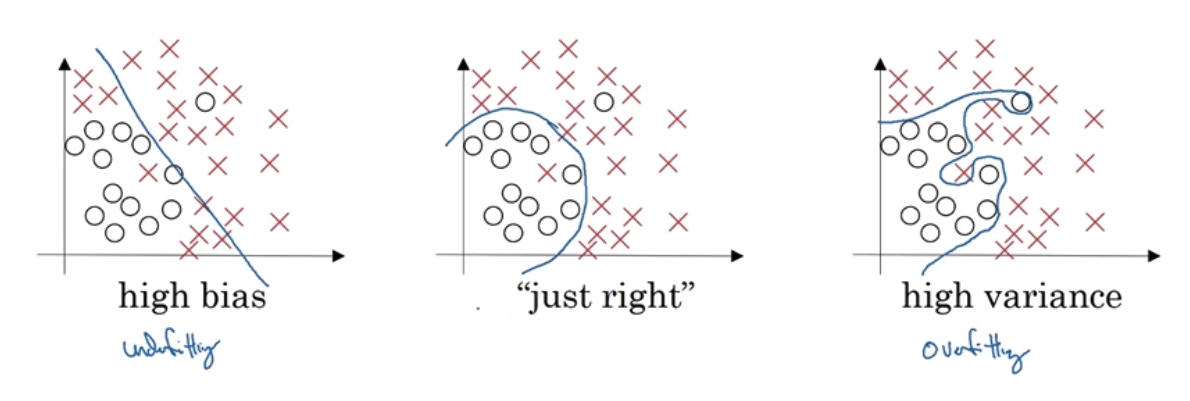
\includegraphics[width=\textwidth]{Images/Bias-Variance.png}
	\caption{Bias and Variance}
	\label{fig:17}
\end{figure}
\FloatBarrier

\subsubsection*{Bias and Variance Intuition}
\begin{itemize}[leftmargin=*, nosep]
    \item \textbf{High Bias:} Underfitting the data (e.g., a simple linear model for complex data). The model performs poorly on the training set.
    \item \textbf{High Variance:} Overfitting the data (e.g., a highly complex model fitting every point). The model performs well on the training set but poorly generalizes to the dev/test set.
    \item \textbf{``Just Right'' Model:} A model with moderate complexity that balances bias and variance.
\end{itemize}

\subsubsection*{Diagnosing Bias and Variance}
\begin{itemize}[leftmargin=*]
    \item Use \textbf{training set error} and \textbf{development (dev) set error}:
    \begin{itemize}
        \item High training error and similar dev error $\rightarrow$ \textbf{High Bias} (underfitting).
        \item Low training error but much higher dev error $\rightarrow$ \textbf{High Variance} (overfitting).
        \item High training error and much higher dev error $\rightarrow$ \textbf{High Bias and High Variance}.
        \item Low training and dev errors $\rightarrow$ \textbf{Low Bias and Low Variance}.
    \end{itemize}
    \item Examples:
	\begin{itemize}
	    \item \textbf{High Variance:} Training error = 1\%, Dev error = 11\%. Model overfits the training data and doesn’t generalize well.
	    \item \textbf{High Bias:} Training error = 15\%, Dev error = 16\%. Model underfits the data.
	    \item \textbf{High Bias and High Variance:} Training error = 15\%, Dev error = 30\%. Model underfits and poorly generalizes.
	    \item \textbf{Low Bias and Low Variance:} Training error = 0.5\%, Dev error = 1\%. Model performs well on both sets.
	\end{itemize}
\end{itemize}

Depending on whether the issue is high bias, high variance, or both, different approaches can be used to improve the model. By evaluating training and dev set errors, you can diagnose whether your model has bias, variance, or both issues. This diagnosis guides the next steps for improving model performance.

% ---------------- Basic Recipe for Machine Learning ----------------------%
\subsection*{Basic Recipe for Diagnosing and Addressing Bias and Variance in Machine Learning}

This note outlines a systematic approach to diagnose and address bias and variance in machine learning algorithms, particularly neural networks. By leveraging tools like training and development set performance, we can iteratively improve model performance using a structured recipe.
\begin{enumerate}
    \item Look at the \textbf{training set performance} to identify high \textbf{bias}:
    \begin{itemize}
        \item High bias: The model does not fit the training data well.
        \item Remedies for high bias:
        \begin{itemize}
            \item Use a larger network (more hidden layers or units).
            \item Train for a longer duration.
            \item Experiment with advanced optimization algorithms.
            \item Explore different neural network architectures (less systematic, may or may not help).
        \end{itemize}
    \end{itemize}
    \item Look at the \textbf{dev set performance} to identify high \textbf{variance}:
    \begin{itemize}
        \item High variance: The model performs well on the training set but poorly on the dev set.
        \item Remedies for high variance:
        \begin{itemize}
            \item Gather more training data (if feasible).
            \item Apply regularization techniques.
            \item Experiment with more appropriate neural network architectures.
        \end{itemize}
    \end{itemize}
\end{enumerate}

\subsubsection{Iterative Process}
\begin{enumerate}
    \item Start with an initial model.
    \item Diagnose whether the issue is high bias, high variance, or both.
    \item Focus on addressing the identified issue:
    \begin{itemize}
        \item For high bias, prioritize fitting the training set well.
        \item For high variance, ensure the model generalizes to the dev set.
    \end{itemize}
    \item Repeat until achieving both low bias and low variance.
\end{enumerate}

\subsubsection{Modern Deep Learning and Bias-Variance Tradeoff}
\begin{itemize}
    \item In earlier eras, reducing bias often increased variance and vice versa (\textbf{bias-variance tradeoff}).
    \item Modern tools and techniques, such as:
    \begin{itemize}
        \item Larger networks with appropriate regularization reduce bias without significantly increasing variance.
        \item More data reduces variance without much impact on bias.
    \end{itemize}
    \item This flexibility has made deep learning especially effective for supervised learning problems.
    \item Regularization helps reduce variance while minimally increasing bias.
    \item If the network is sufficiently large, the increase in bias is often negligible.
\end{itemize}

\subsubsection{Key Takeaways}
\begin{itemize}
    \item Understanding whether your algorithm suffers from high bias, high variance, or both guides the corrective measures.
    \item Use training and dev set performance as diagnostic tools.
    \item Modern machine learning tools allow for systematic improvement of bias and variance independently.
    \item Larger networks and more data are often key to reducing bias and variance, provided regularization is appropriately applied.
\end{itemize}

% ---------------- Regularizing your Neural Network ----------------------%
\subsection{Regularizing your Neural Network}
Regularization is a key technique to reduce overfitting (high variance) in neural networks. While obtaining more training data is another effective method, it is often not feasible due to cost or availability. Regularization, however, is a practical alternative and is widely used. Below is a breakdown of how it works in logistic regression and neural networks.

% ---------------- Regularization in Logistic Regression ----------------------%
\subsection*{Regularization in Logistic Regression}
\subsubsection*{Cost Function with Regularization}
In Logistic Regression, recall that we try to minimize the cost function $J$ where $w$ and $b$ in the logistic regression, are the parameters. The original cost function \( J \) includes the sum of individual losses over the training examples. So $w$ is an $n_x$-dimensional parameter vector, and $b$ is a real number. i.e., $w \in \mathbb{R}^{n_x}, b \in \mathbb{R}$.
\begin{equation}
J (w, b) = \frac{1}{m} \sum_{i=1}^m \mathcal{L} (y^{(i)}, \hat{y}^{(i)})
\end{equation}

To add regularization, we add the regularization parameter or penalty term
    \[
    J = \frac{1}{m} \sum_{i=1}^m \mathcal{L} (y^{(i)}, \hat{y}^{(i)}) + \frac{\lambda}{2m} ||w||_2^2,
    \]
    where:
    \begin{itemize}
        \item \( \lambda \) is the \textbf{regularization parameter}.
        \item \( ||w||_2^2 = \sum_{j=1}^{n_x} w_j^2 \) = \( w^Tw \) is the squared L2 norm of the weight vector \( w \).
    \end{itemize}

\subsubsection{Why Regularize \( w \) and Not \( b \)}
\begin{itemize}
    \item Most parameters are in \( w \), making it more impactful.
    \item \( b \) is a single scalar and contributes minimally to overfitting, so it's often omitted.
\end{itemize}

\subsubsection{Types of Regularization}
\begin{itemize}
    \item \textbf{L2 Regularization}: Adds \( \frac{\lambda}{2m} ||w||^2 \), the most commonly used form.
    \item \textbf{L1 Regularization}: Adds \( \frac{\lambda}{2m} \sum_{j=1}^{n_x} |w_j| \) = \( \frac{\lambda}{2m} ||w||_1 \)  promoting sparsity (many \( w_j = 0 \)). This can compress models but is less common for neural networks.
\end{itemize}

\subsubsection{Tuning \( \lambda \)} 
\begin{itemize}
    \item Chosen via a development set or cross-validation.
    \item Balances training set performance with reduced overfitting.
\end{itemize}

% ---------------- Regularization in Neural Networks ----------------------%
\subsection*{Regularization in Neural Networks}

In a Neural Network, you have a cost function that is a function of all your parameters \(w^{[1]}, b^{[1]}, \cdots, w^{[L]}, b^{[L]}\) where \( L \) is 
the numbers of layers in our network. The cost function is the sum of the losses over \( m \) training examples. To add regularization, we added \( \frac{\lambda}{2m} \) 
of sum over all parameters \( w \). This regularization is called the squared norm. The cost function with regularization adds a term to penalize large weights:
    \[
    J = \frac{1}{m} \sum_{i=1}^m \text{Loss}(y^{(i)}, \hat{y}^{(i)}) + \frac{\lambda}{2m} \sum_{l=1}^L ||w^{[l]}||_F^2,
    \]

\begin{equation}
J(w^{[1]}, b^{[1]}, \cdots, w^{[L]}, b^{[L]}) = \frac{1}{m} \sum_{i=1}^m \mathcal{L} (\hat{y}^{(i)}, y^{(i)}) + \frac{\lambda}{2m} \sum_{\ell=1}^L ||w^{[\ell]}||^2
\end{equation}
where:
\begin{itemize}
\item \( ||w^{[\ell]}||_F^2 = \sum_{i=1}^{n^{[\ell]}} \sum_{j=1}^{n^{[\ell-1]}} (w_{ij}^{[\ell]})^2 \) where the shape of \( w \) is (\(n^{[\ell]}, n^{[\ell-1]} \))
\end{itemize}

\( ||w^{[\ell]}||^2 \) is is the \textbf{Frobenius norm} of the weight matrix \( w^{[l]} \).

% ---------------- Gradient Descent Update with Regularization ----------------------%
\subsection*{Gradient Descent Update with Regularization}
\begin{itemize}
    \item Compute \( dw^{[l]} \) from backpropagation, then add \( \frac{\lambda}{m} w^{[l]} \) to account for regularization.
    \item Update rule: 
    \[
    w^{[l]} = w^{[l]} - \alpha \left( dw^{[l]} + \frac{\lambda}{m} w^{[l]} \right).
    \]
    \item Equivalent to scaling \( w^{[l]} \) by a factor slightly less than 1 in each iteration, hence the term \textbf{weight decay}.
\end{itemize}

We can implement gradient descent with regularization. 
\begin{align*}
dW^{[l]} &= \frac{1}{m} dZ^{[l]} \cdot A^{[l-1]^T} + \frac{\lambda}{m} W^{[l]} \\
W^{[l]} &:= W^{[l]} - \alpha \cdot dW^{[l]} ~\text{i.e.,} \\
W^{[l]} &:= W^{[l]} - \alpha \left( \frac{1}{m} dZ^{[l]} \cdot A^{[l-1]^T} + \frac{\lambda}{m} W^{[l]} \right) \\
	&= W^{[l]} - \frac{\alpha \lambda}{m} W^{[l]} - \alpha \cdot \frac{1}{m} dZ^{[l]} \cdot A^{[l-1]^T} 
\end{align*}

L2 norm regularization is also called ``weight decay''. It is called weight decay because \( W^{[l]} - \frac{\alpha \lambda}{m} W^{[l]} = (1 - \frac{\alpha \lambda}{m} ) W^{[l]} \) \\
\textbf{Note:} \\
\[ \frac{\partial J}{\partial w^{[l]}} = dW^{[l]} \]

% ---------------- Why Does Regularization Help with Overfitting? ----------------------%
\subsection*{Why Does Regularization Help with Overfitting?}
Regularization helps to mitigate overfitting and reduce variance by penalizing large weight values in the cost function. Let's explore the intuition behind this process and understand why it works effectively.
 \begin{enumerate}
\item \textbf{High Bias, High Variance, and the ``Just Right'' Case} \\
Consider a large and deep neural network prone to overfitting. The cost function for such a network is:
\[
J(W, b) = \text{(sum of losses)} + \frac{\lambda}{m} \|W\|_F^2,
\]
where \(\|W\|_F^2\) represents the Frobenius norm of the weight matrices \(W\). The regularization term penalizes large weights.
\begin{itemize}
\item Effect of High \(\lambda\):
	\begin{itemize}[leftmargin=*, nosep]
	\item A large \(\lambda\) strongly encourages \(W\) to be close to zero. This reduces the impact of many hidden units, effectively simplifying the network.
	\item With many hidden units ``zeroed out'', the network behaves like a smaller, simpler neural network or even a logistic regression model. This moves the network from the overfitting (high variance) regime to a state closer to the high-bias case.
	\item At an intermediate value of \(\lambda\), the network achieves a ``just right'' balance, avoiding both overfitting and underfitting.
	\end{itemize}

\item Reduced Impact of Hidden Units:
	\begin{itemize}[leftmargin=*, nosep]
	\item While \(\lambda\) doesn't entirely zero out weights, it reduces their magnitude, resulting in a simpler network that is less prone to overfitting.
	\end{itemize}
\end{itemize}
\item \textbf{Role of Activation Functions (e.g., \(\tanh\))} \\
Consider the \(\tanh(z)\) activation function, defined as \(g(z) = \tanh(z)\):
\begin{itemize}
\item When \(z\) is small (due to small weights \(W\)), \(\tanh(z)\) operates in its linear regime.
\item In this case, each layer of the neural network approximates a linear transformation, simplifying the network into a nearly linear model.
\item A deep network with linear activation functions computes a linear function, which cannot model highly complex decision boundaries. Thus, the model avoids overfitting.
\end{itemize}
\end{enumerate}

\subsection*{Why Regularization Works}
Regularization helps prevent overfitting by:
\begin{itemize}[nosep]
    \item Penalizing large weights, forcing the model to learn simpler, more generalizable patterns.
    \item Acting as a constraint that keeps the parameter values small, reducing the model's capacity to overfit.
\end{itemize}

% ---------------- Dropout regularization ----------------------%
\subsection*{Dropout regularization}
Dropout is a regularization technique used to prevent overfitting in neural networks. The idea is to randomly ``drop'' or deactivate a subset of neurons during training, forcing the network to learn more robust representations.

\subsubsection*{How Does Dropout Work?}
\textbf{Training Phase}
\begin{enumerate}
    \item For each layer, randomly remove nodes with a probability defined by \texttt{keep\_prob}. For example, with \texttt{keep\_prob = 0.8}, there is an 80\% chance of keeping a node and a 20\% chance of removing it.
    \item After deciding which nodes to drop, remove all outgoing connections from these nodes.
    \item Train the network with this reduced structure for each batch.
    \item Repeat the random dropout process for every new batch, creating different network configurations during training.
\end{enumerate}

\textbf{``Inverted Dropout'' Implementation}
\begin{itemize}
    \item A dropout mask \( d^l \) is created for layer \( l \) using a random matrix, where each element is set to 1 with probability \texttt{keep\_prob} and 0 otherwise.
    \item Multiply the activations \( a^l \) by \( d^l \) element-wise to deactivate certain neurons.
    \item Scale the activations by dividing by \texttt{keep\_prob} to ensure the expected value remains consistent.
\end{itemize}

\textbf{Test Phase}
\begin{itemize}
    \item Dropout is not used at test time. Instead, the full network is used, and the activations are not scaled, ensuring deterministic predictions.
\end{itemize}

\subsubsection*{Why Does Dropout Work?}
\begin{itemize}
    \item Dropout trains multiple smaller networks by randomly deactivating neurons. This prevents over-reliance on specific neurons and encourages the network to generalize better.
    \item It reduces co-adaptation of neurons, making the model more robust to variations in data.
\end{itemize}

\subsubsection{Other Regularization Methods}
Other techniques in addition to L2 regularization and drop out regularization for reducing over fitting in your neural network includes:
\begin{itemize}[nosep]
\item \textbf{Data Augmentation:} Expanding the training dataset by applying transformations to existing data such as random crops, flipping, rotations, zooms, or distortion of an image.
\item \textbf{Early Stopping:} Stop training when the dev set error starts increasing, even if the training cost is still decreasing. \\
	- Automatically selects effective parameter magnitudes without exhaustive hyperparameter search.
\end{itemize}

% ---------------- Setting Up Optimization Problem ----------------------%
\subsection{Setting Up Optimization Problem}
% ---------------- Normalizing Inputs ----------------------%
\subsection*{Normalizing Inputs}
When training a neural network, one of the techniques to speed up your training is if you \emph{normalize} your inputs. Normalization standardize the input features by setting all the features to a mean of 0 and variance of 1.  Normalization helps the cost function have more symmetric, spherical contours, making optimization smoother and faster. Normalization is crucial if feature ranges differ significantly. If features are already on similar scales, normalization may have less impact but rarely harms performance.

% ---------------- Vanishing/Exploding Gradients ----------------------%
\subsection*{Vanishing and Exploding Gradients in Deep Neural Networks}
In very deep networks, gradients can become \textbf{exponentially large (exploding)} or \textbf{exponentially small (vanishing)} as they propagate through layers. This leads to training challenges:
    \begin{itemize}
        \item \textit{Exploding gradients}: Outputs grow exponentially with the number of layers.
        \item \textit{Vanishing gradients}: Gradients shrink exponentially, causing gradient descent to take tiny steps and slow learning.
    \end{itemize}

This happens because the output $\hat{Y}$ is influenced by the product of weight matrices ($W_1, W_2, \dots, W_L$). If the weights is:
    \begin{itemize}
        \item \textit{Slightly $> 1$}: Activations or gradients grow exponentially ($1.5^L$).
        \item \textit{Slightly $< 1$}: Activations or gradients shrink exponentially ($0.5^L$).
    \end{itemize}

The impact on training in deep neural network is that training very deep networks (e.g., 150+ layers) becomes difficult:
    \begin{itemize}
        \item \textit{Exploding gradients}: Cause instability.
        \item \textit{Vanishing gradients}: Prevent learning due to tiny updates.
    \end{itemize}

A \textbf{careful choice of weight initialization} can significantly reduce the problem, though not eliminate it entirely.

% ---------------- Weight Initialization for Deep Networks ----------------------%
\subsection*{Weight Initialization for Deep Networks}
Vanishing and Exploding Gradients are significant issues in training very deep neural networks. A \textit{careful choice of weight initialization} can mitigate these problems, though not eliminate them entirely. Weight initialization can help to address the vanishing and exploding gradient problem.

\textbf{Single Neuron Example} \\
A single neuron with \( n \) input features (\( x_1, x_2, \dots, x_n \)) computes:
\[
z = \sum_{i=1}^n w_i x_i, \quad b = 0 \quad \text{(bias ignored)}.
\]
To prevent \( z \) from becoming too large or too small:
\begin{itemize}
    \item The larger \( n \), the smaller \( w_i \) should be.
    \item A reasonable choice is to set the variance of \( w \) to:
    \[
    \text{Var}(w) = \frac{1}{n}.
    \]
\end{itemize}

\textbf{Deep Network Generalization} \\
For a layer \( l \), where each unit has \( n^{(l-1)} \) inputs:
\[
W = \text{np.random.randn}(\text{shape}) \times \sqrt{\frac{1}{n^{(l-1)}}}.
\]

\textbf{ReLU Activation} \\
If using a ReLU activation function (\( g(z) = \max(0, z) \)):
\begin{itemize}
    \item Set variance to:
    \[
    \text{Var}(w) = \frac{2}{n}.
    \]
    \item Practical initialization formula:
    \[
    W = \text{np.random.randn}(\text{shape}) \times \sqrt{\frac{2}{n^{(l-1)}}}.
    \]
\end{itemize}

\textbf{Tanh Activation} \\
For Tanh (\( g(z) = \tanh(z) \)):
\begin{itemize}
    \item Set variance to:
    \[
    \text{Var}(w) = \frac{1}{n}.
    \]
    \item Known as \textbf{Xavier Initialization}:
    \[
    W = \text{np.random.randn}(\text{shape}) \times \sqrt{\frac{1}{n^{(l-1)}}}.
    \]
\end{itemize}

In summary: \\
\begin{enumerate}
    \item \textbf{Default Weight Initialization:}
    \begin{itemize}
        \item Use \( \sqrt{\frac{2}{n}} \) for ReLU.
        \item Use \( \sqrt{\frac{1}{n}} \) for Tanh.
    \end{itemize}
    \item \textbf{Tuning Variance:}
    \begin{itemize}
        \item While rarely a primary focus, variance can be treated as a hyperparameter.
        \item A multiplier to these formulas can sometimes improve training.
    \end{itemize}
\end{enumerate}

Proper weight initialization helps control the scale of weights and gradients in deep networks. This reduces the likelihood of vanishing or exploding gradients, enabling more efficient training of deep architectures.

% ---------------- Optimization Algorithms ----------------------%
\section{Optimization Algorithms}
Large datasets slow training, but efficient optimization algorithms, like \emph{mini-batch gradient descent}, can significantly improve performance. Vectorization efficiently computes on all $m$ training examples simultaneously by stacking data into matrices $X$ (shape: $n_x \times m$) and $Y$ (shape: $1 \times m$). For large $m$ (e.g., millions), processing the entire dataset per gradient descent step becomes slow. 

\textbf{Batch Gradient Descent} processes the entire dataset per step (slower with large datasets) whereas \textbf{Mini-Batch Gradient Descent} takes multiple steps per epoch (e.g., 5,000 steps for $b = 1,000$ mini-batches in 1 epoch). An Epoch is one full pass through the training set. Mini-batch gradient descent allows faster training, making it the standard for large datasets.

In Mini-Batches, we:
\begin{itemize}[nosep]
    \item Divide the training set into smaller subsets (\textbf{mini-batches}) of size $b$ (e.g., $b = 1,000$).
    \item Each mini-batch $t$ contains $X^{\{t\}}$ (inputs) and $Y^{\{t\}}$ (outputs), with dimensions:
    \[
    X^{\{t\}}: n_x \times b, \quad Y^{\{t\}}: 1 \times b
    \]
    \item Example: With 5 million samples and $b = 1,000$, there are $5,000$ mini-batches.
	\[
	X = 
	\begin{bmatrix}
	x^{(1)} & x^{(2)} & x^{(3)} & \cdots & x^{(1000)} | & x^{(1001)} & \cdots & x^{(2000)} | & \cdots & x^{(m)}
	\end{bmatrix}
	\]
	
	\vspace{-3.0em}

	\[
	\underbrace{\phantom{
	\begin{bmatrix}
	x^{(1)} & x^{(2)} & x^{(3)} & \cdots & x^{(1000)}
	\end{bmatrix}
	}}_{X^{\{1\}}}
	\quad
	\underbrace{\phantom{
	\begin{bmatrix}
	x^{(1001)} & \cdots & x^{(2000)}
	\end{bmatrix}
	}}_{X^{\{2\}}}
	\quad
	\cdots
	\quad
	\underbrace{\phantom{
	\begin{bmatrix}
	x^{(m)}
	\end{bmatrix}
	}}_{X^{\{5000\}}}
	\]

	\[
	Y = 
	\begin{bmatrix}
	y^{(1)} & y^{(2)} & y^{(3)} & \cdots & y^{(1000)} | & y^{(1001)} & \cdots & y^{(2000)} | & \cdots & y^{(m)}
	\end{bmatrix}
	\]
	
	\vspace{-3.0em}

	\[
	\underbrace{\phantom{
	\begin{bmatrix}
	y^{(1)} & y^{(2)} & y^{(3)} & \cdots & y^{(1000)}
	\end{bmatrix}
	}}_{Y^{\{1\}}}
	\quad
	\underbrace{\phantom{
	\begin{bmatrix}
	y^{(1001)} & \cdots & y^{(2000)}
	\end{bmatrix}
	}}_{Y^{\{2\}}}
	\quad
	\cdots
	\quad
	\underbrace{\phantom{
	\begin{bmatrix}
	y^{(m)}
	\end{bmatrix}
	}}_{Y^{\{5000\}}}
	\]
\end{itemize}

% ---------------- Mini-Batch Gradient Descent ----------------------%
\subsection{Mini-Batch Gradient Descent}
In Mini-batch gradient descent, we process one mini-batch at a time instead of the entire dataset, allowing faster gradient descent steps.
\begin{itemize}[nosep]
    \item Training consists of:
    \begin{enumerate}
        \item \textbf{Forward Propagation} on $X^{\{t\}}$.
        \item \textbf{Cost Calculation} ($J^{\{t\}}$): Average loss + regularization.
        \item \textbf{Backpropagation}: Compute gradients for $J^{\{t\}}$ using $X^{\{t\}}, Y^{\{t\}}$.
        \item \textbf{Parameter Updates}: Update weights $W$ and biases $b$ using:
        \[
        W^{[l]} \gets W^{[l]} - \alpha \cdot \frac{\partial J^{\{t\}}}{\partial W^{[l]}}
        \]
    \end{enumerate}
    \item A single pass through all mini-batches = \textbf{1 epoch}.
\end{itemize}

To run mini-batch on the training set, we would have:
\begin{lstlisting}
for t =  $1,  \cdots, 5000$: 
	$\quad$ implement 1 step of gradient descent using $X^{[t]}, Y^{[t]}$ (as if $m = 1000$)
	
	$\quad$ Forward prop on $X^{[t]}$
	$\hspace{4em} Z^{[1]} = W^{[1]}.X^{t} + b^{[1]}$
	$\hspace{4em} A^{[1]} = g^{[1]}(Z^{[1]})$
	$\hspace{4em}$		.
	$\hspace{4em}$		.
	$\hspace{4em}$		.
	$\hspace{4em}$		.
	$\hspace{4em} A^{[L]} = g^{[L]}(Z^{[L]})$
	$\quad$ Compute cost $J^{[t]}= \frac{1}{1000} * \sum_{i=1}^l \mathcal{L} (\hat{y}^{(i)}, y^{(i)}) + \frac{\lambda}{2*1000} \sum_{\ell=1}^L ||w^{[\ell]}||^2_F$
	$\quad$ Backprop to compute gradient w.r.t. $J^{[t]}$ (using $X^{\{t\}}, Y^{\{t\}}$)
	$\quad$ $W^{[l]} := W^{[l]} - \alpha \cdot \frac{\partial J^{\{t\}}}{\partial W^{[l]}} = W^{[l]} - \alpha \cdot dW^{[l]}$
	$\quad$ $b^{[l]} := b^{[l]} - \alpha \cdot \frac{\partial J^{\{t\}}}{\partial b^{[l]}} = b^{[l]} - \alpha \cdot db^{[l]}$
\end{lstlisting}

The code above is doing 1 epoch of training .i.e., a single pass through the training set which allows you to take 5,000 gradient descent steps.

We perform Mini-Batch Gradient Descent because it:
\begin{itemize}
    \item Balances the extremes of \textbf{batch gradient descent} (entire dataset) and \textbf{stochastic gradient descent} (one sample at a time).
    \item Speeds up training while maintaining efficient vectorized operations.
\end{itemize}

\textbf{Fig. \ref{fig:18}} shows the Batch versus Mini-batch Gradient Descent.
\begin{figure}[h]
	\centering
	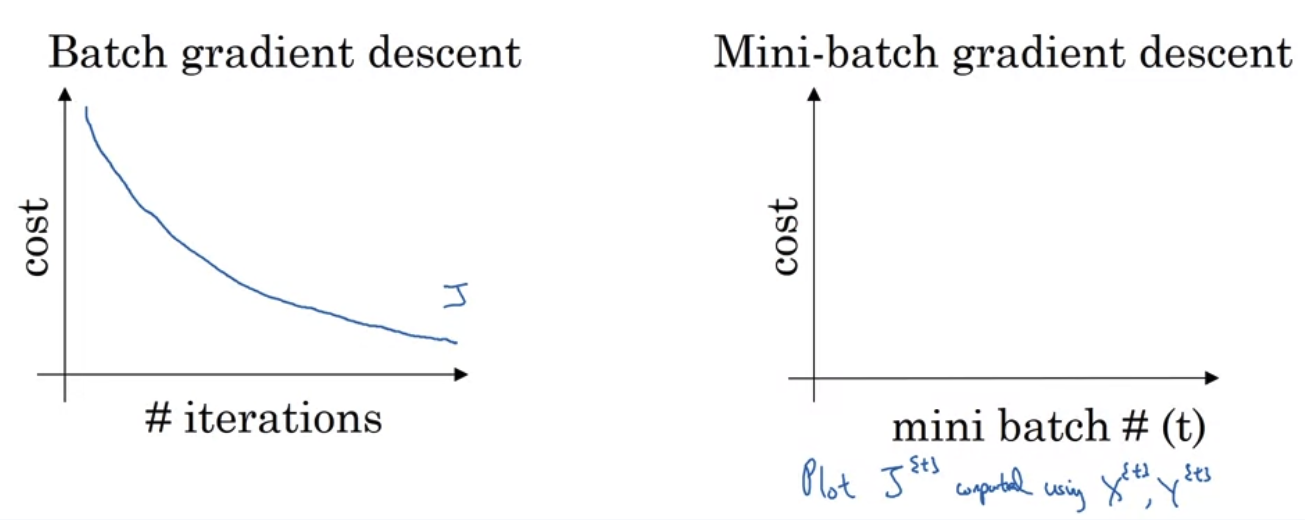
\includegraphics[width=0.85\textwidth]{Images/Batch vs Mini-batch GD.png}
	\caption{Training with Mini-batch Gradient Descent}
	\label{fig:18}
\end{figure}
\FloatBarrier

\subsubsection{Training with Mini-batch Gradient Descent}
In summary:
\begin{itemize}[nosep]
\item Gradient Descent Overview
\begin{itemize}
    \item \textbf{Batch Gradient Descent:} Processes the \textit{entire training set} during each iteration.
    \item The cost function \( J \) should \textbf{decrease consistently} across iterations. If it increases, it may indicate an issue, such as a learning rate that is too large.
\end{itemize}

\item Mini-Batch Gradient Descent
\begin{itemize}
    \item Divides the training set into smaller \textit{mini-batches}, enabling gradient descent steps after processing parts of the training set.
    \item The cost function \( J \) becomes \textbf{noisier} (due to variations across mini-batches) but \textbf{trends downward} over multiple epochs.
\end{itemize}

\item Stochastic Gradient Descent (SGD)
\begin{itemize}
    \item Special case where the \textbf{mini-batch size = 1}.
    \item Processes one training example per iteration, resulting in extremely \textbf{noisy updates}.
    \item SGD often oscillates near the minimum and does not fully converge.
\end{itemize}
\end{itemize}

\subsubsection{Choosing the Mini-Batch Size}
\begin{itemize}[nosep]
    \item \textbf{Batch Gradient Descent} (\( m \),  entire training set):
    \begin{itemize}
        \item Suitable for \textbf{small datasets} (e.g., less than 2000 examples).
        \item Slow for large datasets due to high computational cost per iteration.
    \end{itemize}
    \item \textbf{Stochastic Gradient Descent} (size = 1):
    \begin{itemize}
        \item Highly inefficient due to lack of vectorization and increased noise.
    \end{itemize}
    \item \textbf{Mini-Batch Gradient Descent} (\( 1 < size < m \)):
    \begin{itemize}
        \item Balances computational efficiency and noise reduction.
        \item Typical sizes: \textbf{64, 128, 256, 512} (powers of 2 are preferred for memory efficiency).
    \end{itemize}
\end{itemize}

\subsubsection{Practical Guidelines}
\begin{itemize}[nosep]
    \item Use \textbf{batch gradient descent} for \textbf{small datasets} (e.g., less than 2000 examples).
    \item For larger datasets, try mini-batch sizes in the range of \textbf{64 to 512}, or up to \textbf{1024}.
    \item Ensure that the mini-batch fits in CPU/GPU memory.
    \item Fine-tune the mini-batch size as a \textbf{hyperparameter} to optimize the cost function.
\end{itemize}

\subsubsection{Performance Considerations}
\begin{itemize}[nosep]
    \item Mini-batches allow for \textbf{vectorization}, speeding up computations compared to SGD.
    \item Enables progress without needing to process the entire training set, leading to \textbf{faster convergence}.
\end{itemize}

% ---------------- Algorithms Faster than Gradient Descent ----------------------%
\subsection{Algorithms Faster than Gradient Descent}
The algorithms faster than gradient descent include:
\begin{itemize}[nosep]
\item Gradient Descent with Momentum
\item RMSprop
\item Adam Optimization Algorithm
\end{itemize}

Some important concept that are useful in these faster algorithms include Exponentially Weighted Averages and Bias Correction.

% ---------------- Exponentially Weighted Averages ----------------------%
\subsection*{Exponentially Weighted Averages}
\textbf{Exponentially Weighted Averages (EWA)} are foundational for understanding advanced optimization algorithms that improve upon gradient descent. Also known as \textbf{Exponentially Weighted Moving Averages (EWMA)} in statistics. EWAs are useful for smoothing noisy data and capturing trends.

\subsubsection{Computing the Exponentially Weighted Average (EWA)}
\begin{itemize}
    \item Initialize \( V_0 = 0 \).
    \item Update formula for \( V_t \) (EWA at day \( t \)):
    \[
    V_t = \beta V_{t-1} + (1 - \beta)\theta_t
    \]
    where:
    \begin{itemize}
        \item \( \beta \): Smoothing parameter (e.g., \( \beta = 0.9 \)).
        \item \( \theta_t \): Temperature on day \( t \).
    \end{itemize}
    \item Intuition:
    \begin{itemize}
        \item \( \beta \): Controls the weight of the previous value \( V_{t-1} \).
        \item \( 1 - \beta \): Weight assigned to the current temperature \( \theta_t \).
    \end{itemize}
\end{itemize}

\subsubsection{Impact of \(\beta\) on EWA Behavior}
\begin{itemize}
    \item For \( \beta = 0.9 \):
    \begin{itemize}
        \item Averages over approximately \( \frac{1}{1 - \beta} = 10 \) days of temperatures.
        \item Produces a red curve (smooth but responsive to changes).
    \end{itemize}
    \item For \( \beta = 0.98 \):
    \begin{itemize}
        \item Averages over approximately \( \frac{1}{1 - \beta} = 50 \) days.
        \item Produces a green curve (very smooth but slower to adapt to changes).
        \item High \( \beta \) values cause \textbf{latency} due to increased weight on previous values.
    \end{itemize}
    \item For \( \beta = 0.5 \):
    \begin{itemize}
        \item Averages over approximately \( \frac{1}{1 - \beta} = 2 \) days.
        \item Produces a yellow curve (highly responsive to changes but noisy).
    \end{itemize}
\end{itemize}

\begin{figure}[h]
    \centering
    % First subfigure
    \begin{subfigure}[b]{0.45\textwidth}
        \centering
        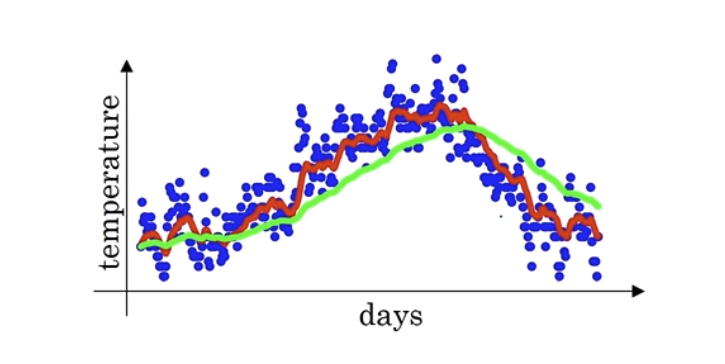
\includegraphics[width=\textwidth]{Images/Exponentially Weighted Averages.png}
        \caption{Exponentially Weighted Averages}
        \label{fig:19}
    \end{subfigure}
    \hfill
    % Second subfigure
    \begin{subfigure}[b]{0.45\textwidth}
        \centering
        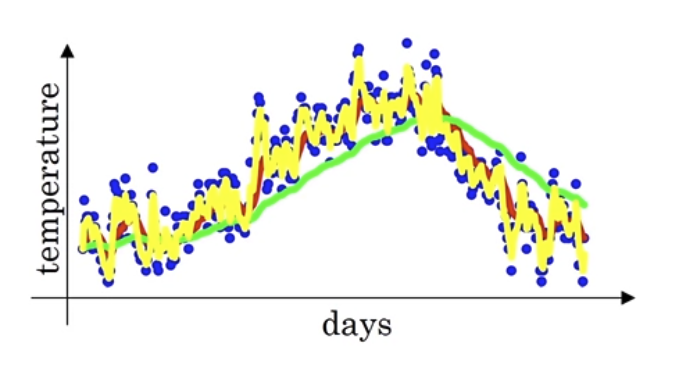
\includegraphics[width=\textwidth]{Images/EWA for beta=0.5.png}
        \caption{Exponentially Weighted Averages for beta of 0.5}
        \label{fig:20}
    \end{subfigure}
    \caption{Comparison of Exponentially Weighted Averages}
    \label{fig:side_by_side}
\end{figure}
\FloatBarrier

\subsubsection{Trade-offs in Smoothing}
\begin{itemize}
    \item High \( \beta \) (e.g., \( 0.98 \)):
    \begin{itemize}
        \item Smoother curve (less noisy).
        \item Slower adaptation to changes (lag).
    \end{itemize}
    \item Low \( \beta \) (e.g., \( 0.5 \)):
    \begin{itemize}
        \item Faster adaptation to changes.
        \item Noisier curve (more susceptible to outliers).
    \end{itemize}
    \item Choosing an optimal \( \beta \):
    \begin{itemize}
        \item Balances smoothness and responsiveness.
        \item Often a hyperparameter tuned for the application.
    \end{itemize}
\end{itemize}

\subsubsection{Bias Correction in Exponentially Weighted Average}
Typically, EWAs are initialized with \( V_0 = 0\).  For \( V_1 \):  
     \[
     V_1 = \beta V_0 + (1 - \beta) \theta_1 = (1 - \beta) \theta_1
     \]  
Since \( V_0 = 0 \), this leads to an initial value for \( V_1 \) that is much smaller than \( \theta_1 \).  As we propagate from \(V_1\) to \(V_t\), the weights are biased toward earlier terms, resulting in underestimates for the initial days.  

To correct the bias, divide \( V_t \) by \( 1 - \beta^t \):  
   \[
   \hat{V}_t = \frac{V_t}{1 - \beta^t} 
   \]  
This normalization removes the downward bias during the early phase. After applying bias correction, \( \hat{V}_t \) becomes a proper weighted average of temperatures (\( \theta_1, \theta_2, \dots \)) without the initial downward bias.  

Bias correction is critical for obtaining better estimates early on.  In later stages, both corrected and uncorrected EWAs converge to the same values.  


% ---------------- Gradient Descent with Momentum ----------------------%
\subsection*{Gradient Descent with Momentum}
Gradient descent with momentum, (also called \emph{Momentum}), often speeds up the optimization process compared to standard gradient descent. The core idea is to compute an exponentially weighted average of the gradients and use this to update the weights.

In Standard Gradient Descent, oscillations in the vertical direction slow progress and limit the learning rate. Also a larger learning rate can lead to overshooting or divergence.To solve this, we make use of Gradient Descent with momentum.

To run Gradient Descent with Momentum:
\begin{lstlisting}
Initialize $v_{dW}$ and $v_{db}$ as zero vectors with same dimensions as $W$ and $b$.
Hyperparameters are $\alpha$ and $\beta$
Select $\beta = 0.9$ (commom choice for hyperparameter $\beta$)
On iteration $t$: 
	$\quad$ Compute the gradient $dW$ and $db$ on current mini-batch
	$\quad$ Update the moving averages:
	$\hspace{4em} v_{dW} = \beta v_{dW} + (1 - \beta) dW$
	$\hspace{4em} v_{db} = \beta v_{db} + (1 - \beta) db $
	$\quad$ Update the weights using the smoothed gradients:
	$\hspace{4em} W := W - \alpha v_{dW} $
	$\hspace{4em} b := b - \alpha v_{db} $		
\end{lstlisting}
This algorithm reduces oscillations in the vertical direction by averaging out gradients, enabling a smoother descent and increases speed in the horizontal direction, allowing faster convergence.

% ---------------- RMSProp Algorithm ----------------------%
\subsection*{RMSProp Algorithm}
RMSprop (\textbf{Root Mean Square Propagation}) is an optimization algorithm designed to speed up gradient descent by addressing issues such as oscillations in parameter updates.

The steps in RMSprop are:
\begin{lstlisting}
On iteration $t$: 
	$\quad$ Compute the gradient $dW$ and $db$ on current mini-batch
	$\quad$ Keep an exponentially weighted average of the squared gradients:
	$\hspace{4em} S_{dW} = \beta_2 S_{dW} + (1 - \beta_2) \cdot (dW^2) $
	$\hspace{4em} S_{db} = \beta_2 S_{db} + (1 - \beta_2) \cdot (db^2) $
	$\hspace{4em}$Here, squaring is an element-wise operation.
	$\quad$ Update the parameters:
	$\hspace{4em} W = W - \frac{\alpha \cdot dW}{\sqrt{S_{dW}} + \epsilon} $
	$\hspace{4em} b = b - \frac{\alpha \cdot db}{\sqrt{S_{db}} + \epsilon} $	
\end{lstlisting}
where \( \epsilon \) is a small value (e.g., \( 10^{-8} \)) added for numerical stability.

\subsubsection*{Intuition Behind RMSprop}
Gradient descent can suffer from \textbf{oscillations in the vertical direction} (e.g., parameter \( b \)) while trying to progress in the horizontal direction (e.g., parameter \( W \)). RMSprop slows learning in the \textbf{vertical direction} and maintains or accelerates learning in the \textbf{horizontal direction}.

\begin{itemize}[nosep]
    \item \textbf{Horizontal direction (parameter \( W \)):}
    \begin{itemize}
        \item \( S_{dW} \) is relatively small since gradients (\( dW \)) are small.
        \item Updates in this direction are \textbf{not slowed down}.
    \end{itemize}
    \item \textbf{Vertical direction (parameter \( b \)):}
    \begin{itemize}
        \item \( S_{db} \) is relatively large due to large gradients (\( db \)).
        \item Updates in this direction are \textbf{damped}, reducing oscillations.
    \end{itemize}
\end{itemize}

The net effect is that RMSprop smoothens the learning process and allows faster convergence.

The advantages of RMSprop are:
\begin{itemize}[nosep]
    \item Reduces oscillations in problematic directions.
    \item Allows the use of a \textbf{larger learning rate} (\( \alpha \)) without divergence.
    \item Speeds up mini-batch gradient descent.
\end{itemize}

In practice:
\begin{itemize}[noitemsep, topsep=0pt]
    \item RMSprop is effective in \textbf{high-dimensional parameter spaces}.
    \item To prevent instability, always add a small \( \epsilon \) in the denominator.
    \item Common default for \( \beta_2 \): \( 0.9 \).
\end{itemize}

RMSprop is a powerful optimization tool that works well for neural network training. Combining RMSprop with momentum can further improve performance.

% ---------------- Adam Optimization Algorithm ----------------------%
\subsection*{Adam Optimization Algorithm}
Adam (\textbf{Adaptive Moment Estimation}) optimization algorithm combines the effect of gradient descent with momentum together with gradient descent with RMSprop.

\begin{lstlisting}
Initialize $v_{dW}=0, S_{dW} =0,  v_{db}=0, S_{db} =0$ as zero vectors with same dimensions as $W$ and $b$.
On iteration $t$: 
	$\quad$ Compute the gradient $dW$ and $db$ on current mini-batch
	$\quad$ Perform $\emph{momentum}$ update on the moving averages:
	$\hspace{4em} v_{dW} = \beta_1 v_{dW} + (1 - \beta_1) dW$
	$\hspace{4em} v_{db} = \beta_1 v_{db} + (1 - \beta_1) db $
	$\quad$ Perform $\emph{RMSprop}$ update of the squared gradients:
	$\hspace{4em} S_{dW} = \beta_2 S_{dW} + (1 - \beta_2) \cdot (dW^2) $
	$\hspace{4em} S_{db} = \beta_2 S_{db} + (1 - \beta_2) \cdot (db^2) $
	$\quad$ Implement bias correction on $V$ and $S$:
	$\hspace{4em} v^{corrected}_{dW} = \frac{v_{dW}}{1 - {\beta_1}^t} $
	$\hspace{4em} v^{corrected}_{db} = \frac{v_{db}}{1 - {\beta_1}^t} $
	$\hspace{4em} S^{corrected}_{dW} = \frac{S_{dW}}{1 - {\beta_2}^t} $
	$\hspace{4em} S^{corrected}_{db} = \frac{S_{db}}{1 - {\beta_2}^t} $
	$\quad$ Update the parameters:
	$\hspace{4em} W := W - \frac{\alpha \cdot v^{corrected}_{dW}}{\sqrt{S^{corrected}_{dW}} + \epsilon} $
	$\hspace{4em} b := b - \frac{\alpha \cdot v^{corrected}_{db}}{\sqrt{S^{corrected}_{db}} + \epsilon} $	
\end{lstlisting}

The Hyperparameters choice are:
\begin{itemize}[label={\ding{224}}]
	\item \(\alpha\): needs to be tuned
	\item \(\beta_1\): 0.9 \(\qquad \longrightarrow (dW)\)
	\item \(\beta_2\): 0.999 \(\quad \longrightarrow (dW^2)\)
	\item \(\epsilon\): \(10^{-8}\)
\end{itemize}

\subsubsection{Learning Rate Decay}
One of the things that might help speed up your learning algorithm is to slowly reduce your learning rate over time. The way to reduce the learning rate over time is to use a \textbf{learning rate decay}.  Suppose you are using mini-batch gradient descent with a small mini-batch size (e.g., 64 or 128 examples). During training:
\begin{itemize}[noitemsep, topsep=0pt]
    \item The gradient descent steps will be noisy, and the algorithm may oscillate around the minimum rather than converge.
    \item If the learning rate (\( \alpha \)) is fixed, the algorithm might wander and never fully converge due to mini-batch noise.
\end{itemize}

By slowly reducing \( \alpha \):
\begin{itemize}[noitemsep, topsep=0pt]
    \item At the start of training (when \( \alpha \) is large), the algorithm learns faster with bigger steps.
    \item As training progresses and \( \alpha \) decreases, the steps become smaller, allowing the algorithm to oscillate closer to the minimum.
\end{itemize}

The intuition is that during the initial phase, large steps are beneficial, but as training approaches convergence, smaller steps are needed for fine-tuning.

The formula for learning rate decay \(\alpha\) is:
\[ \alpha = \frac{1}{1+\text{decayRate}*\text{epochNumber}}*\alpha_0\]
where:
\begin{itemize}[noitemsep, topsep=0pt]
    \item \( \alpha_0 \): Initial learning rate.
    \item \text{decay\_rate}: A hyperparameter that controls how fast the learning rate decreases.
    \item \text{epoch\_num}: Current epoch number.
\end{itemize}

Other learning rate decay methods used to decay the learning rate includes:
\begin{enumerate}
    \item \textbf{Exponential Decay:}
    \[
    \alpha = \alpha_0 \cdot 0.95^{\text{epoch\_num}}
    \]
    where \( 0.95 \) is a constant (less than 1) that exponentially decays the learning rate.

    \item \textbf{Square Root Decay:}
    \[
    \alpha = \frac{\alpha_0}{\sqrt{\text{epoch\_num}}}
    \]

    \item \textbf{Discrete Staircase Decay:}
    Reduce \( \alpha \) by half after a fixed number of epochs.

    \item \textbf{Manual Decay:}
    For long training sessions, monitor the training progress and manually decrease \( \alpha \) when needed. This works well for small-scale experiments.
\end{enumerate}

In practice:
\begin{itemize}[noitemsep, topsep=0pt]
	\item Learning rate decay adds hyperparameters (e.g., \(\alpha_0\) and decay rate).
	\item Tuning \(\alpha\) as a fixed value usually has a bigger impact than decay.
	\item Decay is useful for fine-tuning after good \(\alpha\) initialization.
\end{itemize}

% ---------------- Hyperparameter Tuning, Batch Normalization and Programming Frameworks ----------------------%
\section{Hyperparameter Tuning, Batch Normalization and Programming Frameworks}

% ---------------- Hyperparameter Tuning and Key Hyperparameters in Neural Networks ----------------------%
\subsection{Hyperparameter Tuning and Key Hyperparameters in Neural Networks}
\begin{enumerate}[nosep]
    \item \textbf{Most Important: Learning Rate ($\alpha$)}  
    \begin{itemize}
        \item Critical for convergence; tune this first.
    \end{itemize}
    \item \textbf{Second Tier:}
    \begin{itemize}
        \item Momentum term ($\beta$, default: 0.9).
        \item Mini-batch size (affects optimization efficiency).
        \item Number of hidden units.
    \end{itemize}
    \item \textbf{Third Tier:}
    \begin{itemize}
        \item Number of layers.
        \item Learning rate decay.
    \end{itemize}
    \item \textbf{Adam Optimization Hyperparameters:}  
    \begin{itemize}
        \item Defaults ($\beta_1 = 0.9$, $\beta_2 = 0.999$, $\epsilon = 10^{-8}$) generally work well and rarely need tuning.
    \end{itemize}
\end{enumerate}

\subsection*{Random Sampling vs. Grid Search}
\begin{itemize}[nosep]
    \item \textbf{Grid Search:}
    \begin{itemize}
        \item Systematically samples a fixed grid of hyperparameter values.
        \item Effective for a small number of hyperparameters.
        \item Inefficient when some hyperparameters (e.g., $\alpha$) are more critical than others.
    \end{itemize}
    \item \textbf{Random Sampling (Preferred):}
    \begin{itemize}
        \item Samples random points in the hyperparameter space.
        \item Provides richer exploration of important hyperparameters.
        \item Works better when the importance of hyperparameters varies.
    \end{itemize}
\end{itemize}

\subsubsection*{Coarse-to-Fine Search}
\begin{enumerate}[noitemsep, topsep=0pt]
    \item Start with a broad, random sample across the hyperparameter space.
    \item Identify regions where hyperparameters perform well.
    \item Refine the search by zooming into these regions and sampling more densely.
\end{enumerate}

The key takeaways is that:
\begin{itemize}[noitemsep, topsep=0pt]
    \item Prioritize tuning learning rate ($\alpha$) first, followed by other hyperparameters.
    \item Use \textbf{random sampling} for richer exploration.
    \item Apply a \textbf{coarse-to-fine search} to focus resources efficiently.
\end{itemize}

% ---------------- Using an Appropriate Scale to pick Hyperparameters ----------------------%
\subsection*{Using an Appropriate Scale to pick Hyperparameters}
\begin{enumerate}[noitemsep, topsep=0pt]
\item Random Sampling Over Hyperparameters
\begin{itemize}
    \item Sampling at random is more efficient than grid search, but it doesn’t mean sampling uniformly across valid values.
    \item The appropriate scale must be used to explore hyperparameters effectively.
\end{itemize}

\item Sampling on a Linear Scale
\begin{itemize}
    \item Suitable for hyperparameters like:
    \begin{itemize}
        \item Number of hidden units $n[l]$: e.g., range $50$–$100$.
        \item Number of layers $L$: e.g., values $2$, $3$, $4$.
    \end{itemize}
    \item For these, uniform sampling or grid search over the range is reasonable.
\end{itemize}

\item Sampling on a Logarithmic Scale
\begin{itemize}
    \item Necessary for hyperparameters like the learning rate $\alpha$:
    \begin{itemize}
        \item Example: range $0.0001$ to $1$.
        \item On a linear scale, $90\%$ of sampled values might fall between $0.1$ and $1$, ignoring smaller values like $0.0001$.
    \end{itemize}
    \item Use log scale to distribute resources effectively:
    \begin{itemize}
        \item Convert range $[10^{-4}, 10^0]$ to $[-4, 0]$ by taking log base $10$.
        \item Sample $r$ uniformly in $[-4, 0]$, then set $\alpha = 10^r$.
    \end{itemize}
\end{itemize}

\item Sampling for $\beta$ (Exponential Weighted Average)
\begin{itemize}
    \item Example: $\beta$ in the range $[0.9, 0.999]$.
    \item Direct linear sampling results in uneven exploration:
    \begin{itemize}
        \item Sensitivity increases for $\beta$ values close to $1$.
    \end{itemize}
    \item Solution:
    \begin{itemize}
        \item Focus on $1 - \beta$, with range $[0.1, 0.001]$.
        \item Transform to log scale: $10^{-1}$ to $10^{-3}$.
        \item Sample $r$ in $[-3, -1]$, set $1 - \beta = 10^r$, and $\beta = 1 - 10^r$.
    \end{itemize}
\end{itemize}
\end{enumerate}

We sample on a log scale because:
\begin{itemize}[noitemsep, topsep=0pt]
    \item Small changes in hyperparameters like $\beta$ near critical regions (e.g., close to $1$) have significant effects.
    \item Log scaling ensures resources are allocated to regions with greater sensitivity.
\end{itemize}

The key takeaways is that:
\begin{itemize}[noitemsep, topsep=0pt]
    \item Select the correct scale (linear or log) for each hyperparameter.
    \item Even if the wrong scale is used, a coarse-to-fine search can mitigate inefficiencies.
    \item Organize the search to refine promising ranges iteratively.
\end{itemize}

% ---------------- Batch Normalization ----------------------%
\subsection{Batch Normalization}
Batch Normalization (Batch Norm), introduced by Sergey Ioffe and Christian Szegedy, is a technique that simplifies hyperparameter tuning and makes training neural networks more robust. It allows for training very deep networks by normalizing intermediate layer values.

% ---------------- Normalizing Inputs in Neural Networks ----------------------%
\subsection*{Normalizing Inputs in Neural Networks}
When training models like logistic regression, normalizing the input features \(X\) helps speed up learning:
\begin{itemize}[noitemsep, topsep=0pt]
    \item \textbf{Steps:}
    \begin{enumerate}[noitemsep, topsep=0pt]
        \item Compute the mean: 
        \[
        \mu = \frac{1}{m} \sum_{i=1}^m X^{(i)}
        \]
        \item Subtract the mean from the dataset: 
        \[
        X_{\text{mean}} = X - \mu
        \]
        \item Compute the variance: 
        \[
        \sigma^2 = \frac{1}{m} \sum_{i=1}^m (X^{(i)} - \mu)^2
        \]
        \item Normalize the data:
        \[
        X_{\text{norm}} = \frac{X - \mu}{\sqrt{\sigma^2 + \epsilon}}
        \]
        Here, \(\epsilon\) is a small constant for numerical stability.
    \end{enumerate}
\end{itemize}

Normalizing inputs makes the optimization contours more circular, improving algorithms like gradient descent.

% ---------------- Batch Norm for Hidden Layers ----------------------%
\subsection*{Batch Norm for Hidden Layers}
Batch Norm normalizes activations or intermediate values \(z\) in hidden layers:
\begin{itemize}[noitemsep, topsep=0pt]
    \item This normalization ensures efficient training of parameters \(w, b\), e.g., \(w_3, b_3\).
    \item It generalizes input normalization to intermediate layers (\(a_1, a_2, \dots\)).
\end{itemize}

\subsubsection{Implementing Batch Norm}
For a hidden layer with values \(z^{(1)}, z^{(2)}, \dots, z^{(m)}\):
\begin{enumerate}[noitemsep, topsep=0pt]
    \item \textbf{Compute the Mean:}
    \[
    \mu = \frac{1}{m} \sum_{i=1}^m z^{(i)}
    \]
    \item \textbf{Compute the Variance:}
    \[
    \sigma^2 = \frac{1}{m} \sum_{i=1}^m (z^{(i)} - \mu)^2
    \]
    \item \textbf{Normalize \(z^{(i)}\):}
    \[
    z^{(i)}_{\text{norm}} = \frac{z^{(i)} - \mu}{\sqrt{\sigma^2 + \epsilon}}
    \]
    where \(\epsilon\) ensures numerical stability.
    \item \textbf{Scale and Shift:}
    Introduce learnable parameters \(\gamma\) and \(\beta\) to allow flexibility:
    \[
    \tilde{z^{(i)}} = \gamma \cdot z^{(i)}_{\text{norm}} + \beta
    \]
    \(\gamma\) controls the variance, and \(\beta\) controls the mean.
\end{enumerate}

We use \(\gamma\) and \(\beta\) because:
\begin{itemize}[noitemsep, topsep=0pt]
    \item Without \(\gamma\) and \(\beta\), hidden units would have fixed mean (0) and variance (1).
    \item Learnable \(\gamma\) and \(\beta\) enable the network to optimize mean and variance.
    \item For example, with sigmoid activation, avoiding values clustered around 0 can better utilize its nonlinearity.
\end{itemize}

\subsubsection{Implementation and Integration}
\begin{itemize}[noitemsep, topsep=0pt]
    \item Replace each layer’s \(z_i\) values with the scaled and shifted values \(\tilde{z}_i\).
    \item During backpropagation, update \(\gamma\) and \(\beta\) using gradient descent or other optimization algorithms.
\end{itemize}

Batch Norm applies normalization to deeper layers, not just input features. It ensures standardized mean and variance for hidden units, controlled by \(\gamma\) and \(\beta\). Batch Norm Works because:
\begin{itemize}[noitemsep, topsep=0pt]
    \item Stabilizes learning by preventing activations from becoming too large or small.
    \item Reduces internal covariate shift (changes in layer input distributions during training).
    \item Improves gradient flow, enabling efficient optimization of deep networks.
\end{itemize}

% ---------------- Batch Normalization in a Deep Network ----------------------%
\subsection*{Fitting Batch Normalization into a Deep Network}
Batch Normalization (Batch Norm) normalizes the intermediate outputs (activations) in a neural network, stabilizing learning and improving convergence speed. It is applied after computing the linear transformation \( Z \) and before applying the activation function \( A \).

Each layer of a neural network computes:
\begin{align*}
    Z &= W \cdot A_{\text{prev}} + B \quad \text{(Linear transformation)} \\
    A &= g(Z) \quad \text{(Activation function application)}
\end{align*}

\subsubsection{With Batch Norm:}
\begin{itemize}[noitemsep, topsep=0pt]
    \item Compute \( Z \), then normalize it to \( \tilde{Z} \) using the mean and variance of the mini-batch.
    \item Rescale \( \tilde{Z} \) with learnable parameters \( \beta \) (shift) and \( \gamma \) (scale):
    \[
    \tilde{Z} = \gamma \cdot Z_{\text{normalized}} + \beta
    \]
    \item Pass \( \tilde{Z} \) through the activation function to compute \( A \).
\end{itemize}

\subsubsection{Steps in Batch Norm:}
\begin{enumerate}[noitemsep, topsep=0pt]
    \item Compute \( Z \) for the current layer.
    \item Calculate the mean and variance of \( Z \) across the current mini-batch.
    \item Normalize \( Z \):
    \[
    Z_{\text{normalized}} = \frac{Z - \mu}{\sqrt{\sigma^2 + \epsilon}}
    \]
    \item Rescale and shift \( Z_{\text{normalized}} \) to get \( \tilde{Z} \) using \( \gamma \) and \( \beta \).
    \item Feed \( \tilde{Z} \) into the activation function to compute \( A \).
\end{enumerate}

\subsubsection{Parameter Updates:}
Additional parameters introduced for Batch Norm are \( \beta \) (shift) and \( \gamma \) (scale) for each layer. \\
During training:
\begin{align*}
    \beta &:= \beta - \eta \cdot \frac{\partial L}{\partial \beta} \\
    \gamma &:= \gamma - \eta \cdot \frac{\partial L}{\partial \gamma}
\end{align*}
where \( \eta \) is the learning rate. Updates can also use optimizers like Adam or RMSprop.

Since Batch Norm centers \( Z \) to have a mean of 0, the bias term \( \beta \) becomes redundant and can be removed.

\subsubsection{Dimension of Parameters:}
If a layer has \( n_L \) units:
\begin{itemize}[noitemsep, topsep=0pt]
    \item Dimensions of \( Z \): \( n_L \times 1 \) (for one example).
    \item Dimensions of \( \beta \) and \( \gamma \): \( n_L \times 1 \).
\end{itemize}

% ---------------- Training Process with Batch Norm ----------------------%
\subsection*{Training Process with Batch Norm}
Batch Norm is applied to each mini-batch independently by computing the mean and variance of \( Z \) using only the examples in the current mini-batch. The training process with Batch Norm includes:
\begin{enumerate}[noitemsep, topsep=0pt]
    \item \textbf{Forward Propagation:}
    \begin{itemize}
        \item Compute \( Z \), apply Batch Norm to get \( \tilde{Z} \), and compute activations \( A \).
    \end{itemize}
    \item \textbf{Backward Propagation:}
    \begin{itemize}
        \item Compute gradients for \( W \), \( \gamma \), and \( \beta \).
        \item Update all parameters using gradient descent or advanced optimization algorithms.
    \end{itemize}
\end{enumerate}

\subsubsection{Why Does Batch Norm Work?}
\begin{itemize}[noitemsep, topsep=0pt]
    \item \textbf{Speeding Up learning} - Normalizing input features \( X \) to have mean 0 and variance 1 can speed up learning.
    \item \textbf{Reducing Covariate Shift} - Batch Norm minimizes these shifts by ensuring that the hidden unit values in each layer (e.g., \(Z_2\)) maintain a consistent mean and variance across training, making it easier for deeper layers to learn.
    \item \textbf{Stabilizing Hidden Unit Distributions} - Batch Norm keeps the mean and variance of the hidden unit values stable. For example, even as parameters in earlier layers change, Batch Norm ensures that the later layers still see input values with similar distributions.
    \item \textbf{Regularization Effect} - Batch Norm introduces slight noise during training because the mean and variance are computed on mini-batches rather than the entire dataset. This noise adds a small regularization effect similar to dropout.
    \item \textbf{Handling Mini-Batches at Test Time} - During training, Batch Norm computes the mean and variance for each mini-batch. However, during testing, predictions may be made on individual examples, not mini-batches. To address this, Batch Norm uses running averages of the mean and variance computed during training for consistent predictions.
\end{itemize}

% ---------------- Multi-Class Classification ----------------------%
\subsection{Multi-Class Classification}
\subsection*{Binary vs Multi-Class Classification}
\begin{itemize}[noitemsep, topsep=0pt]
    \item \textbf{Binary classification:} Used when there are two possible labels (e.g., 0 or 1). Example: Is it a cat or not?
    \item \textbf{Multi-class classification:} Used when there are multiple possible classes (e.g., cats, dogs, baby chicks, or ``none of the above'').
    \begin{itemize}
        \item Classes are indexed as $0, 1, 2, \ldots, C-1$, where $C$ is the total number of classes.
        \item Example: Cats = 1, Dogs = 2, Baby chicks = 3, and ``Other'' = 0.
    \end{itemize}
\end{itemize}

% ---------------- Softmax Regression ----------------------%
\subsection*{Generalization of Logistic Regression: Softmax Regression}
\begin{itemize}[noitemsep, topsep=0pt]
    \item Logistic regression generalizes to multi-class classification through \textbf{Softmax regression}.
    \item For $C$ classes, the output layer will have $C$ units, each representing the probability of a class given the input $x$.
\end{itemize}

\newpage
\subsubsection{Softmax Layer}
\begin{itemize}[noitemsep, topsep=0pt]
    \item \textbf{Output vector $\hat{y}$:} A $C \times 1$ dimensional vector where:
    \begin{itemize}
        \item Each element represents the probability of one class.
        \item Probabilities sum to 1.
    \end{itemize}
\end{itemize}

The Softmax Activation Function is computed using the steps below:
\begin{enumerate}[noitemsep, topsep=0pt]
    \item Compute $z^{[L]} = W^{[L]} \cdot a^{[L-1]} + b^{[L]}$ (linear component of layer $L$).
    \item Compute $t = e^{z^{[L]}}$ element-wise (temporary variable).
    \item Normalize $t$ to sum to 1:
    \[
    a^{[L]}_i = \frac{t_i}{\sum_{j=1}^{C} t_j}
    \]
    where $a^{[L]}$ is the output of the Softmax layer.
\end{enumerate}

For example: \\
Given $z^{[L]} = [5, 2, -1, 3]$:
\begin{itemize}
    \item $t = [e^5, e^2, e^{-1}, e^3] = [148.4, 7.4, 0.37, 20.1]$
    \item Normalize: 
    \[
    \hat{y} = \frac{t}{\sum t} \approx [0.842, 0.042, 0.002, 0.114]
    \]
\end{itemize}

A \textbf{Softmax classifier} without hidden layers creates linear decision boundaries between classes. For example: with $C = 3$, three linear boundaries partition the input space into regions corresponding to the classes. A deeper neural network with hidden layers can model \textbf{non-linear decision boundaries}, making it suitable for complex datasets.

\begin{itemize}
    \item \textbf{Sigmoid vs. Softmax:}
    \begin{itemize}
        \item Sigmoid handles binary classification (outputs a scalar probability for one class).
        \item Softmax handles multi-class classification (outputs a vector of probabilities across classes).
    \end{itemize}
    \item Softmax ensures all probabilities sum to 1, normalizing the outputs.
\end{itemize}

\subsubsection{Applications of Softmax}
\begin{itemize}
    \item Used for tasks requiring multi-class predictions (e.g., image classification, natural language processing).
    \item Can model increasingly complex decision boundaries when combined with deeper architectures.
\end{itemize}

% ---------------- Chapter 3. Structuring Machine Learning Projects ----------------------%
\chapter{Structuring Machine Learning Projects} \label{ch:3}
% ---------------- Machine Learning Strategy ----------------------%
\section{Machine Learning Strategy}
\textbf{Orthogonalization in Machine Learning} is a process where individual ``knobs'' in a system are designed to control only one specific aspect of that system's behavior. This design philosophy makes it easier to diagnose issues and tune performance in machine learning systems. Here is how we can apply it to machine learning.
\begin{itemize}[noitemsep, topsep=0pt]
\item \textbf{Training Set Performance} - If the system isn’t performing well on the training set, tune parameters like network size or optimization algorithm.
\item \textbf{Generalization to Dev Set} - Use knobs like regularization or increasing training data to improve performance on the dev set.
\item \textbf{Generalization to Test Set} - If the test set performance is lacking, expand the dev set to avoid overfitting.
\item \textbf{Real-World Performance} - Adjust the dev set distribution or the cost function if performance doesn’t translate to real-world success.
\end{itemize}

The challenges of non-orthogonalized controls are:
\begin{itemize}[noitemsep, topsep=0pt]
\item Techniques like early stopping affect multiple aspects (e.g., training set fit and dev set performance), making optimization harder.
\item Orthogonalized knobs simplify tuning by isolating their effects on specific performance areas.
\end{itemize}

By clearly identifying bottlenecks (e.g., training, dev set, test set, or real-world performance) and having orthogonalized controls to address each, you streamline the optimization process and enhance system performance.

% ---------------- Single Number Evaluation Metrics ----------------------%
\subsection{Single Number Evaluation Metrics}
Using a single real number evaluation metric accelerates progress in machine learning by providing a quick and clear way to compare different models or approaches. It simplifies decision-making when trying out new ideas, hyperparameters, or learning algorithms.

Machine learning often involves an iterative process:
\begin{enumerate}[noitemsep, topsep=0pt]
    \item Developing an idea.
    \item Coding and implementing it.
    \item Running experiments.
    \item Using experiment results to refine the idea.
\end{enumerate}
This cycle repeats to improve the algorithm. Having a single evaluation metric enables quick comparisons, speeding up this process.

\textbf{For example:}
\begin{itemize}[noitemsep, topsep=0pt]
    \item \textbf{Precision:} Measures how many predicted cats are actually cats.  
        \begin{itemize}
            \item Example: If precision = 95\%, 95\% of predicted cats are correct.
        \end{itemize}
    \item \textbf{Recall:} Measures how many actual cats were identified as cats.  
        \begin{itemize}
            \item Example: If recall = 90\%, 90\% of actual cats were correctly recognized.
        \end{itemize}
\end{itemize}

Although both metrics are important, using them separately can lead to ambiguity when comparing classifiers (e.g., one has higher precision while the other has higher recall).

\textbf{The solution is: F1 Score} \\
The F1 score combines precision and recall into a single metric using the harmonic mean:
\[
F1 = \frac{2}{\frac{1}{P} + \frac{1}{R}}
\]
It balances the tradeoff between precision and recall, enabling a clear comparison of classifiers.

% ---------------- Satisficing and Optimizing Metrics ----------------------%
\subsection{Satisficing and Optimizing Metrics}
When it is difficult to combine all desired metrics into a single evaluation metric, it can be helpful to set up \textbf{optimizing} and \textbf{satisficing} metrics. This approach allows you to prioritize certain metrics while ensuring others meet minimum thresholds.

\subsubsection{For Example: Classification Accuracy and Running Time}
Suppose you care about two metrics for a classifier:
\begin{itemize}[noitemsep, topsep=0pt]
    \item \textbf{Accuracy:} How well the classifier identifies the correct category.
    \item \textbf{Running Time:} The time it takes to classify an image.
\end{itemize}

If we perform a classification task using three different classifiers and the running time for the models are:
\begin{itemize}[noitemsep, topsep=0pt]
    \item Classifier A: 80 ms
    \item Classifier B: 95 ms
    \item Classifier C: 1,500 ms (1.5 s)
\end{itemize}

One approach is to combine these metrics into a single formula, such as:
\[
\text{Overall Metric} = \text{Accuracy} - 0.5 \times \text{Running Time}
\]
However, this may feel artificial or arbitrary. Instead, you can:
\begin{itemize}[noitemsep, topsep=0pt]
    \item \textbf{Optimize Accuracy:} Maximize accuracy.
    \item \textbf{Satisfice Running Time:} Ensure the running time is $\leq 100$ ms.
\end{itemize}

Using this setup, classifier B is the best choice because it maximizes accuracy while meeting the running time threshold.

\textbf{The General Approach is:} \\
For \(N\) metrics:
\begin{itemize}[noitemsep, topsep=0pt]
    \item Select one as the \textbf{optimizing metric} to maximize or minimize.
    \item Set the remaining \(N-1\) metrics as \textbf{satisficing metrics}, where each must meet a predefined threshold.
\end{itemize}

Consider a wake word detection system (e.g., \textit{“Alexa”}, \textit{“Hey Siri”}, \textit{“Ni Hao Baidu”}) used in a Trigger Word Detection System:
\begin{itemize}[noitemsep, topsep=0pt]
    \item \textbf{Accuracy:} Maximize the probability of waking the device when the correct trigger word is spoken.
    \item \textbf{False Positives:} Minimize the number of random wake-ups to at most one per 24 hours.
    \item Accuracy is the \textbf{optimizing metric}.
    \item False positives are the \textbf{satisficing metric}, with the threshold of at most one false positive every 24 hours.
\end{itemize}

In summary, if you care about multiple metrics:
\begin{enumerate}[noitemsep, topsep=0pt]
    \item Select one as the \textbf{optimizing metric}.
    \item Use others as \textbf{satisficing metrics} with thresholds.
    \item Evaluate metrics on training, development (dev), or test sets.
\end{enumerate}

This approach simplifies decision-making, allowing you to select the ``best'' system automatically by focusing on the most important metric while ensuring others meet acceptable thresholds.

% ---------------- Size of the Dev and Test Sets ----------------------%
\subsection{Size of the Dev and Test Sets in the Deep Learning Era}
The way we set up dev and test sets has evolved with the advent of big data and deep learning. Below are the key takeaways:
\begin{enumerate}[label=\textbf{\arabic*.}]
    \item \textbf{Outdated Rules of Thumb:}
    \begin{itemize}
        \item Traditional splits like 70/30 (train/test) or 60/20/20 (train/dev/test) were reasonable when datasets were small (e.g., 100–10,000 examples).
        \item These splits are less relevant for modern machine learning problems with larger datasets.
    \end{itemize}

    \item \textbf{Modern Best Practices:}
    \begin{itemize}
        \item With large datasets (e.g., 1 million examples), it’s reasonable to allocate \textbf{98\% for training} and just \textbf{1\% each for dev and test sets}.
        \item Even 1\% of a million examples provides 10,000 examples, which is often sufficient for evaluation purposes.
    \end{itemize}

    \item \textbf{Purpose of Dev and Test Sets:}
    \begin{itemize}
        \item \textbf{Dev Set:} Used during development to evaluate and select the best model.
        \item \textbf{Test Set:} Used at the end to evaluate the final system and ensure confidence in its performance.
    \end{itemize}

    \item \textbf{Size Guidelines:}
    \begin{itemize}
        \item The test set should be \textbf{large enough} to provide high confidence in the final system's performance but doesn't need to be excessively large.
        \item In some applications, 10,000 or 100,000 examples may suffice for test sets.
    \end{itemize}

    \item \textbf{When to Skip a Test Set:}
    \begin{itemize}
        \item If you’re iterating and tuning on the test set, it’s better to call it a \textbf{dev set}.
        \item In rare cases where overall performance isn't critical, you might only use a train-dev split (no separate test set). However, this is generally \textbf{not recommended}.
    \end{itemize}

    \item \textbf{Focus on Training Data:}
    \begin{itemize}
        \item Deep learning algorithms are data-hungry, so prioritize allocating a \textbf{large fraction of data to training} for better model performance.
    \end{itemize}
\end{enumerate}

In Summary:
\begin{itemize}[noitemsep, topsep=0pt]
    \item The old 70/30 split is outdated in the era of big data. Instead, use \textbf{more data for training} and proportionally less for dev and test sets.
    \item Dev and test sets should be sized based on their purpose:
    \begin{itemize}
        \item \textbf{Dev Set:} Big enough to evaluate and compare ideas effectively.
        \item \textbf{Test Set:} Big enough to ensure confidence in final system performance but doesn’t need to be excessively large.
    \end{itemize}
    \item In rare cases, a train-dev split without a test set may suffice, though it’s not ideal.
\end{itemize}

\begin{thickleftborder}
  \textit{A learning algorithm’s performance can be better than human-level performance but it can never be better than Bayes error.}
\end{thickleftborder}

This is because:
\begin{itemize}[noitemsep, topsep=0pt]
\item \textbf{Bayes error} represents the lowest possible error rate achievable by any model, given the true underlying distribution of the data. It sets a theoretical lower bound on the error.
\item \textbf{Human-level performance} is the level of performance achieved by human experts. In some cases, machine learning algorithms can outperform human-level performance, especially in tasks involving large-scale data or pattern recognition.
\end{itemize}

However, no algorithm can exceed the \textbf{Bayes error}, as it represents the best possible performance based on the available data and model assumptions.

% ---------------- Carrying Out Error Analysis ----------------------%
\section{Carrying Out Error Analysis}
Error analysis is the process of manually examining the mistakes made by a learning algorithm to gain insights into how to improve it.

The key steps in carrying out error analysis are:
\begin{itemize}[noitemsep, topsep=0pt]
    \item Analyze mislabeled examples from the dev set.
    \item Categorize and count errors by type.
    \item Estimate potential improvements for each category.
    \item Prioritize based on potential impact.
\end{itemize}

% ---------------- Handling Incorrectly Labeled Data ----------------------%
\subsection{Handling Incorrectly Labeled Data}
\textbf{Key Concepts}
\begin{itemize}
    \item \textbf{Incorrect Labels vs. Mislabeled Examples:}
    \begin{itemize}
        \item \textit{Incorrectly labeled examples:} Errors in the dataset where the label $Y$ is wrong (e.g., a dog labeled as a cat).
        \item \textit{Mislabeled examples:} Cases where the learning algorithm predicts an incorrect value of $Y$.
    \end{itemize}
\end{itemize}

\subsection*{Handling Incorrect Labels in the Dataset}
\subsubsection{Training Set}
\begin{itemize}
    \item \textbf{Random Errors:}
    \begin{itemize}
        \item Deep learning algorithms are robust to random labeling errors in the training set.
        \item If errors are reasonably random (e.g., accidental keystrokes), fixing them may be unnecessary if the dataset is large and errors are a small percentage.
    \end{itemize}
    \item \textbf{Systematic Errors:}
    \begin{itemize}
        \item Algorithms are less robust to systematic errors (e.g., consistently labeling white dogs as cats).
        \item Fixing systematic errors is critical to prevent biases in the model.
    \end{itemize}
\end{itemize}

\subsubsection{Dev and Test Sets}
\begin{itemize}
    \item \textbf{Impact on Evaluation:}
    \begin{itemize}
        \item Dev and test sets are used to evaluate and select between models. Incorrect labels can lead to flawed conclusions.
    \end{itemize}
    \item \textbf{Error Analysis:}
    \begin{itemize}
        \item Add a column during error analysis to identify incorrectly labeled examples.
        \item Calculate the fraction of errors due to incorrect labels and assess their impact on the dev/test set.
    \end{itemize}
\end{itemize}

\subsection*{Guidelines for Fixing Incorrect Labels}
\subsubsection{When to Fix Incorrect Labels}
\begin{itemize}
    \item If incorrect labels significantly impact the ability to evaluate models (e.g., dev set accuracy differences are small, but incorrect labels distort results), invest time in correcting them.
    \item \textbf{Example:}
    \begin{itemize}
        \item If 6\% of a 10\% error rate is due to incorrect labels, this is 0.6\%. Errors from other causes are 9.4\%, making incorrect labels a smaller priority.
        \item If the error rate decreases to 2\%, but 0.6\% is still from incorrect labels, this now accounts for 30\% of errors, making it more worthwhile to fix them.
    \end{itemize}
\end{itemize}

\subsubsection*{Correcting Incorrect Dev/Test Set}
\begin{itemize}
    \item Apply the same process to both dev and test sets to make sure they come from the same distributions.
    \item Optionally examine examples the algorithm got right to avoid bias in error estimates.
    \item Focus on Dev/Test Sets Over Training Set
	\begin{itemize}
	    \item Correcting labels in the dev/test set is more impactful for evaluation.
	    \item Training set corrections are often less critical unless errors are systematic.
	\end{itemize}
\end{itemize}

Correcting mislabeled data depends on its impact on evaluation and the nature of the errors. Prioritize fixes in dev/test sets if they significantly affect model selection or evaluation. Use error analysis to guide decisions and be willing to manually inspect data for deeper insights.

One of the recommended practice when building a brand new machine learning system is to \textbf{build your first system quickly and then iterate}.

% ---------------- Mismatched Training and Dev/Test Set ----------------------%
\subsection{Mismatched Training and Dev/Test Set}

% ---------------- Training and Testing on Different Distributions ----------------------%
\subsection*{Handling Training and Test Data from Different Distributions}

Deep learning algorithms perform better with larger datasets, even when data sources differ in distribution. Teams often mix data from different distributions into the training set to increase dataset size, even when test and dev sets come from another distribution. Best practices are needed when training and test distributions differ.

\subsubsection*{Example 1: Mobile App Cat Classifier}
\textbf{Scenario:} Building a classifier for user-uploaded photos (mobile app) to detect cats.
\begin{itemize}
    \item \textbf{Mobile app data:} Less professional, 10,000 images.
    \item \textbf{Web data:} High-quality, professionally taken, 200,000 images.
\end{itemize}

\textbf{Options for Splitting Data:}
\begin{enumerate}
    \item \textbf{Option 1: Combine All Data Randomly}
    \begin{itemize}
        \item \textbf{Setup:} Training set: 205,000; Dev/Test sets: 2,500 examples each (randomly mixed).
        \item \textbf{Advantage:} Simplifies management; all sets share the same distribution.
        \item \textbf{Disadvantage:} Dev/Test sets predominantly reflect web data ($\sim 95\%$), not mobile app data.
        \item \textbf{Impact:} Misleads the team to optimize for web data distribution, which is not the end goal.
    \end{itemize}
    
    \item \textbf{Option 2: Keep Dev/Test from Target Distribution}
    \begin{itemize}
        \item \textbf{Setup:}
        \begin{itemize}
            \item Training set: 200,000 web + 5,000 mobile images.
            \item Dev/Test sets: 2,500 mobile app images each.
        \end{itemize}
        \item \textbf{Advantage:} Focuses model optimization on the mobile app distribution, aligning with project goals.
        \item \textbf{Disadvantage:} Training set distribution differs from dev/test set distribution.
        \item \textbf{Outcome:} Better long-term performance despite differing distributions.
    \end{itemize}
\end{enumerate}

\subsubsection*{Example 2: Speech-Activated Rearview Mirror}
\textbf{Scenario:} Building a speech recognition system for a rearview mirror product.
\begin{itemize}
    \item \textbf{Training data:} 500,000 utterances from unrelated sources (smart speakers, keyboards, etc.).
    \item \textbf{Dev/Test data:} 20,000 utterances specific to rearview mirror use cases.
\end{itemize}

\textbf{Options for Splitting Data:}
\begin{enumerate}
    \item \textbf{Option 1:}
    \begin{itemize}
        \item Training set: 500,000 unrelated utterances.
        \item Dev/Test sets: 10,000 utterances each from rearview mirror data.
    \end{itemize}
    \item \textbf{Option 2:}
    \begin{itemize}
        \item Training set: 510,000 utterances (500,000 unrelated + 10,000 rearview mirror).
        \item Dev/Test sets: 5,000 utterances each from rearview mirror data.
    \end{itemize}
    \item \textbf{Impact:} Combining data increases training set size, improving model performance, while retaining dev/test sets specific to the target distribution.
\end{enumerate}

The key takeaways is to:
\begin{itemize}
    \item Use larger datasets even when training distribution differs from test/dev sets.
    \item Ensure dev/test sets align with the target distribution to optimize for end-use scenarios.
    \item Trade-offs exist between dataset size and distribution alignment, but prioritizing the dev/test distribution often leads to better results.
\end{itemize}


% ---------------- Bias and Variance Analysis with Mismatched Data Distributions ----------------------%
\subsection*{Bias and Variance Analysis with Mismatched Data Distributions}

Estimating the bias and variance of a learning algorithm helps prioritize improvements. However, the analysis differs when the training set has a different distribution than the development (dev) and test sets. 

\subsubsection*{Example: Cat Classification}
Assume that:
\begin{itemize}
    \item Human-level (Bayes) error: ~0\%.
    \item Training error: 1\%, Dev error: 10\%.
\end{itemize}

\begin{example}
If your dev data came from the same distribution as your training set, you would say that here you have a large variance problem, that your algorithm's just not generalizing well from the training set which it's doing well on to the dev set, which it's suddenly doing much worse on. 
\end{example}

Here's how to approach this:
\begin{enumerate}
\item \textbf{Same Distribution (Training \& Dev Sets):}
	\begin{itemize}
	    \item Large difference (10\% - 1\%) indicates a variance problem (poor generalization).
	\end{itemize}
     \[
     \text{Large gap between training and dev error} \implies \text{Variance problem.}
     \]
\item \textbf{Different Distribution:}
	\begin{itemize}
	    \item Cannot directly conclude a variance problem.
	    \item E.g., Training images may be clearer, dev images harder.
	\end{itemize}
\end{enumerate}

The solution is to introduce a ``Training-Dev Set'' which is a subset of the training set with the same distribution as the training set, excluded from training. To carry out error analysis, we look at the error of the classifier on the training set, on the training-dev set (same distribution as training data) as well as on the dev set (different distribution).

Assume after analysis, we have:
\begin{itemize}[nosep]
\item \text{Training error: } 1\%
\item \text{Training-dev error: } 9\%,
\item \text{Dev error: } 10\%. 
\end{itemize}

We can conclude that significant increase (9\% - 1\%) indicates a \textbf{variance problem} (poor generalization within the same distribution).

Assume instead that after analysis:
\begin{itemize}[nosep]
\item \text{Training error: } 1\%
\item \text{Training-dev error: } 1.5\%
\item \text{Dev error: } 10\%
\end{itemize}
The Minimal difference (1.5\% - 1\%) suggests \textbf{low variance} and the large jump (10\% - 1.5\%) suggests a data mismatch problem.i.e., the algorithm performs well within the training distribution but poorly on the dev set, indicating a mismatch.

Assume after analysis:
\begin{itemize}[nosep]
\item  \text{Training error: } 10\%
\item  \text{Training-dev error: } 11\%
\item  \text{Dev error: } 12\%
\end{itemize}
The High training error indicates \textbf{avoidable bias}.

If after analysis:
\begin{itemize}[nosep]
\item  \text{Training error: } 10\%
\item  \text{Training-dev error: } 11\%
\item  \text{Dev error: } 20\%
\end{itemize}
We conclude there is an \textbf{High Avoidable bias} (high training error) and \textbf{Data mismatch problem} (large gap between training-dev and dev errors).

Some general principles for key quantities to look for in error analysis are:
\begin{itemize}[nosep]
    \item \textbf{Human-level error:} Approximate Bayes error.
    \item \textbf{Training error:} Measures avoidable bias.
    \item \textbf{Training-dev error:} Measures variance (gap with training error).
    \item \textbf{Dev error:} Measures data mismatch (gap with training-dev error).
    \item \textbf{Test error:} Identifies overfitting to the dev set (gap with dev error).
\end{itemize}

\subsubsection*{Error Analysis Table}
Error values can be organized in a table:
\begin{center}
    % Adjust row spacing by setting \arraystretch
    \renewcommand{\arraystretch}{2.0} % Increase row spacing (1.5x default)
    \begin{tabular}{@{}c c l@{}}
        \toprule
        \textbf{Dataset Type} & \textbf{Error} & \textbf{Conclusion} \\
        \midrule
        Human-level error & 4\% & \multirow{2}{*}{$\bigg\}\begin{array}{l}
        \end{array} \text{Avoidable bias}$} \\
        Training set error & 7\% & \multirow{2}{*}{$\bigg\}\begin{array}{l}
        \end{array} \text{Variance}$} \\
        Training-Dev set error & 10\% & \multirow{2}{*}{$\bigg\}\begin{array}{l}
        \end{array} \text{Data mismatch}$} \\
        Dev error & 12\% & \multirow{2}{*}{$\bigg\}\begin{array}{l}
        \end{array} \text{Overfitting to Dev set}$} \\
        Test error & 12\% & \\
        \bottomrule
    \end{tabular}
\end{center}

\begin{itemize}[nosep]
    \item \textbf{Avoidable Bias:} Gap between human-level and training error.
    \item \textbf{Variance:} Gap between training and training-dev error.
    \item \textbf{Data Mismatch:} Gap between training-dev and dev error.
    \item \textbf{Degree of overfitting to dev set:} Gap between dev and test error. Solution: Use a larger dev set.
\end{itemize}

% ---------------- Addressing Data Mismatch Problems ----------------------%
\subsection*{Addressing Data Mismatch Problems}
\begin{enumerate}
\item Diagnosing Data Mismatch:
\begin{itemize}
    \item If training data differs from dev/test data and error analysis indicates a mismatch:
    \begin{itemize}
        \item Perform manual error analysis to identify differences between training and dev/test sets.
        \item Focus analysis on the dev set to avoid overfitting the test set.
    \end{itemize}
\end{itemize}

\item Identifying and Understanding Errors:
\begin{itemize}
    \item Example: A speech-activated rear-view mirror system:
    \begin{itemize}
        \item Dev set may have noisy in-car data, e.g., car noise.
        \item Training set might lack examples with navigational queries, e.g., street numbers.
    \end{itemize}
    \item Insights into these differences can guide data improvement efforts.
\end{itemize}

\item Strategies to Address Data Mismatch:
\begin{itemize}
    \item Make Training Data More Similar to Dev/Test Data:
    \begin{itemize}
        \item Collect additional data similar to dev/test sets.
        \item Simulate data with key characteristics of dev/test sets.
    \end{itemize}
    \item Example: For noisy in-car speech data:
    \begin{itemize}
        \item Combine clean audio recordings with car noise recordings to synthesize realistic training data.
    \end{itemize}
\end{itemize}

\item Artificial Data Synthesis:
\begin{itemize}
    \item Create synthetic data to match target conditions, e.g., combining audio recordings with background noise or using computer graphics for vision tasks.
    \item Caution:
    \begin{itemize}
        \item Avoid overfitting to a small subset of synthesized data (e.g., reusing one hour of car noise or a limited number of car models).
        \item Ensure synthesized data covers a broad range of scenarios.
    \end{itemize}
\end{itemize}

\item Challenges of Artificial Data Synthesis:
\begin{itemize}
    \item Synthesized data might represent a small portion of the real-world distribution.
    \item Neural networks may overfit to this limited subset, even if it seems realistic to humans.
    \item Example: In self-driving car systems:
    \begin{itemize}
        \item Using computer graphics with only 20 car models may result in overfitting, as real-world car diversity is much greater.
    \end{itemize}
\end{itemize}
\end{enumerate}

The key takeaways is that:
\begin{itemize}[nosep]
    \item Conduct thorough error analysis to understand data distribution differences.
    \item Collect or synthesize more representative training data to align with dev/test sets.
    \item Use artificial data synthesis cautiously to avoid overfitting to narrow subsets.
    \item Despite its challenges, artificial data synthesis can significantly improve performance when applied carefully.
\end{itemize}

% ---------------- Learning from Multiple Tasks ----------------------%
\subsection{Learning from Multiple Tasks}
% ---------------- Transfer Learning ----------------------%
\subsection*{Transfer Learning in Deep Learning}
One of the most powerful ideas in deep learning is the ability to transfer knowledge from one task to another. This is called \textbf{transfer learning}. For example, you could train a neural network to recognize objects (e.g., cats) and use that knowledge to help read x-ray scans. The process involves using what the neural network has learned from a primary task and applying it to a secondary task.

Suppose you train a neural network on an image recognition task:
\begin{itemize}[nosep]
    \item Input: Images (\(X\)) and Labels (\(Y\)) - images of cats, dogs, birds, etc.
    \item Output: A model that recognizes different objects in images.
\end{itemize}

Now, you want to apply this knowledge to a radiology diagnosis task (e.g., reading x-ray scans). The steps are as follows:
\begin{enumerate}[nosep]
    \item \textbf{Remove the last output layer} of the image recognition model.
    \item \textbf{Replace the last layer} with a new randomly initialized layer for radiology diagnosis.
    \item \textbf{Retrain the model} on the radiology dataset.
\end{enumerate}
This approach leverages the low-level features (e.g., detecting edges, curves, and patterns) that the neural network has already learned from the image recognition task.

\subsubsection*{Pre-training and Fine-tuning}
The process of using a pre-trained model (e.g., trained on image recognition) and adapting it to a new task is often referred to as:
\begin{itemize}
    \item \textbf{Pre-training}: Training the neural network on a task (e.g., image recognition) to learn general features.
    \item \textbf{Fine-tuning}: Adapting the pre-trained model to the new task (e.g., radiology diagnosis) by retraining some or all layers.
\end{itemize}
If you have a small dataset for the new task, it's common to only retrain the last few layers. If you have a large dataset, you may choose to retrain the entire model.

\subsubsection*{Transfer Learning in Action}
\begin{itemize}
    \item \textbf{Radiology Example}: A neural network trained on image recognition (e.g., cats, dogs) can be fine-tuned with a small dataset of radiology images to perform diagnosis tasks, as it already knows about image structures like edges and patterns.
    \item \textbf{Speech Recognition Example}: A speech recognition system trained on large amounts of data can be adapted to detect specific ``wake words'' (e.g., ``Alexa'', ``Hey Siri'') by retraining the last layer or layers with a smaller dataset.
\end{itemize}

\subsubsection*{When Does Transfer Learning Make Sense?}
Transfer learning is most effective when:
\begin{itemize}[nosep]
    \item The source task (Task A) and the target task (Task B) have the same input $X$.
    \item You have \textbf{more data for the source task} (e.g., image recognition or speech recognition) than for the target task (e.g., radiology diagnosis or wake word detection).
    \item The tasks share similar inputs, such as both being image-based (for image recognition and radiology) or audio-based (for speech recognition and wake word detection).
    \item Low-level features from the source task can be useful for the target task.
\end{itemize}

For example:
\begin{itemize}[nosep]
    \item If you have a million images for image recognition and only 100 radiology images, the knowledge from image recognition can be transferred to improve radiology diagnosis, even with limited data.
    \item Similarly, if you have 10,000 hours of speech data for a speech recognition system and only 1 hour for wake word detection, transfer learning can help by applying learned features of human speech.
\end{itemize}

\subsubsection*{When Does Transfer Learning Not Make Sense?}
Transfer learning is less useful when:
\begin{itemize}[nosep]
    \item The source task has less data than the target task.
    \item The tasks are not sufficiently related (e.g., transferring from image recognition to radiology diagnosis when you already have enough data for radiology).
    \item The value of each example in the target task is much higher than in the source task.
\end{itemize}
For example, if you have a small number of radiology images and a large amount of data for image recognition, the transfer learning from image recognition may not be helpful, as the radiology task has more valuable and specific data.

In summary, transfer learning is useful when:
\begin{itemize}[nosep]
    \item The tasks share the same input type.
    \item The source task has more data than the target task.
    \item Low-level features learned from the source task are transferable to the target task.
\end{itemize}
This process allows you to build a model for a task with limited data by leveraging knowledge from a related task with more data.


% ---------------- Multi-task Learning ----------------------%
\subsection*{Multi-task Learning}
Multi-task learning (MTL) is an approach where a single neural network is trained to perform multiple tasks simultaneously. Unlike transfer learning, where knowledge gained from one task (Task A) is transferred to a new, related task (Task B), MTL aims to solve several problems at once within the same network. For example, in autonomous vehicles, a neural network can be trained to detect pedestrians, cars, stop signs, and traffic lights simultaneously.

\subsubsection*{Key Concepts of Multi-task Learning}
\begin{itemize}
    \item \textbf{Multiple Labels}: Each input image in MTL can have multiple labels. For instance, an image of a car and a stop sign will have both labels, instead of just one (like in softmax regression).
    \item \textbf{Loss Function}: In MTL, the loss function is computed for each individual task (e.g., pedestrian, car, stop sign, traffic light), and the final loss is the sum of these individual losses.
    \item \textbf{Shared Features}: The network benefits from shared low-level features across tasks. For example, recognizing cars, pedestrians, and stop signs may use similar visual features. This helps improve the overall performance by leveraging shared information.
    \item \textbf{Handling Missing Labels}: MTL can handle missing labels in some images, as it only sums over the labels that are available for each task, ignoring missing values.
\end{itemize}

\subsubsection*{When Does MTL Make Sense?}
\begin{itemize}[nosep]
    \item \textbf{Shared Low-Level Features}: MTL is beneficial when the tasks share common features. For example, detecting traffic-related objects (cars, pedestrians, traffic lights) likely shares common visual features.
    \item \textbf{Data Volume Balance}: MTL works well when the tasks have similar amounts of training data. If some tasks have less data, MTL can leverage the larger data sets from other tasks to improve performance.
    \item \textbf{Network Size}: For MTL to work effectively, a sufficiently large neural network is needed to handle all the tasks simultaneously. If the network is too small, it might not be able to learn all tasks properly, which could hurt performance compared to training separate networks for each task.
\end{itemize}

\subsubsection*{Benefits of MTL}
\begin{itemize}[nosep]
    \item \textbf{Improved Performance}: MTL can outperform training separate networks for each task by sharing learned features, especially when the tasks are related.
    \item \textbf{Efficiency}: Instead of training multiple networks, MTL allows you to train a single model that solves several problems.
\end{itemize}

\subsubsection*{Applications}
MTL is particularly effective in domains like \textbf{computer vision}, where multiple related tasks, such as object detection (e.g., cars, pedestrians, and traffic signs), can be tackled by a single neural network. While transfer learning is more widely used due to its applicability in situations with small data sets, MTL is a powerful tool when the problem involves multiple related tasks.

% ---------------- End-to-End Deep Learning ----------------------%
\subsection{End-to-End Deep Learning}
\subsection*{What is End-to-end Deep Learning}
End-to-end deep learning refers to training a single neural network to handle all stages of a traditional multi-stage processing pipeline. In many domains, like speech recognition and machine translation, deep learning systems now aim to replace traditional feature extraction and processing steps with a single, unified model.

\subsubsection*{Traditional Systems vs. End-to-End Deep Learning}
In traditional machine learning systems, multiple stages of processing are involved. For example, in speech recognition, the process often includes:
\begin{itemize}[nosep]
    \item Feature extraction (e.g., MFCC for audio).
    \item Phoneme detection.
    \item Stringing phonemes to form words.
    \item Generating a transcript.
\end{itemize}

End-to-end deep learning simplifies this by directly mapping the input (e.g., an audio clip) to the output (e.g., a transcript) through a single neural network. This eliminates the need for feature extraction and multiple intermediate stages.

\subsubsection*{Challenges of End-to-End Learning}
End-to-end deep learning is powerful but requires a large amount of data to be effective. For example, in speech recognition, traditional systems may work better with smaller datasets, while the end-to-end approach excels only when vast datasets (e.g., 10,000 to 100,000 hours of audio) are available. Additionally, intermediate approaches, like learning phonemes before learning full words, can be useful in cases with medium-sized datasets.

\subsubsection*{Example: Face Recognition System}
A face recognition turnstile system is a good example of when end-to-end learning is not ideal. A traditional multi-step approach works better here:
\begin{itemize}[nosep]
    \item \textbf{Step 1:} Use face detection algorithms to locate the face in the image.
    \item \textbf{Step 2:} Crop and center the detected face, then feed it into a neural network for identity recognition.
\end{itemize}

This approach is more effective because each step is simpler and has more labeled data available. For instance, there is abundant labeled data for face detection, and companies have millions of images for identity verification tasks.

\subsection*{Comparison with End-to-End Learning in Other Applications}
\subsubsection{Machine Translation}
End-to-end deep learning works well for machine translation because large datasets of paired sentences (e.g., English and French) are readily available, enabling the direct mapping from one language to another.

\subsubsection{Estimating Child's Age from X-rays}
For tasks like estimating the age of a child from an X-ray, a non-end-to-end approach (multi-step) may perform better. In this case:
\begin{itemize}[nosep]
    \item \textbf{Step 1:} Segment the X-ray to identify bones.
    \item \textbf{Step 2:} Use bone length statistics from a database to estimate age.
\end{itemize}
This two-step process works better because the tasks are simpler and sufficient data for each step is available, whereas end-to-end learning would require significantly more data to directly map an X-ray to an age.

End-to-end deep learning offers a simplified system that eliminates the need for hand-designed features and multiple processing steps. However, it is not a one-size-fits-all solution. It works best when large amounts of data are available. In cases where data is limited or tasks are complex, a multi-step approach might be more effective.

\subsection*{Whether to use End-to-end Deep Learning}
End-to-end deep learning can be a powerful method for certain machine learning tasks, but it comes with both benefits and limitations. Here's an overview to guide decision-making:
\subsubsection*{Benefits and Drawbacks of End-to-end deep learning}
\textbf{Benefits:}
\begin{enumerate}
    \item \textbf{Data-Driven}: End-to-end learning allows the data to determine the best function mapping from input (\(X\)) to output (\(Y\)). The neural network learns the most appropriate representations without human-imposed structures.
    \begin{itemize}
        \item \textit{Example}: In speech recognition, phonemes (human-defined units of sound) may not be the best representation. Letting the model learn its own representation can lead to better performance.
    \end{itemize}
    \item \textbf{Less Hand Design}: It minimizes the need for manual feature engineering or designing intermediate components, simplifying the workflow.
\end{enumerate}

\textbf{Drawbacks}
\begin{enumerate}
    \item \textbf{Data Hungry}: This approach requires a large amount of data to learn the complex function from \(X\) to \(Y\). If data is sparse, it may be harder for the model to capture the necessary patterns.
    \begin{itemize}
        \item \textit{Example}: Tasks like face recognition might have enough data for \(X\) (input image) and \(Y\) (identified face), but other tasks may not.
    \end{itemize}
    \item \textbf{Excludes Hand-Designed Components}: While hand-designed components can inject valuable knowledge into a model (especially when data is limited), end-to-end learning doesn't use these components, potentially losing out on human expertise that could improve performance in small datasets.
\end{enumerate}

To decide whether an end-to-end approach is suitable, consider whether you have sufficient data to support learning the required complexity from \(X\) to \(Y\). If the task is relatively simple (e.g., recognizing faces), end-to-end learning can work well with less data. But for more complex tasks (e.g., predicting age from an image), it may require more data.

For example, in autonomous driving:
\begin{itemize}
    \item \textbf{Deep Learning} can detect objects (cars, pedestrians) from sensor inputs (images, lidar).
    \item \textbf{Motion Planning} (non-deep learning) is needed to decide the car’s route and how to execute the steering, acceleration, and braking commands.
\end{itemize}
Thus, while deep learning can work for detection, motion planning and control are better served by specialized algorithms.

End-to-end deep learning is promising for many applications, but it is not a one-size-fits-all solution. If data is abundant and the task can be learned directly, end-to-end learning is effective. However, combining deep learning with other techniques often yields better results, especially in cases of limited data or high complexity.

% ---------------- Chapter 4. Convolutional Neural Networks ----------------------%
\chapter{Convolutional Neural Networks} \label{ch:4}
% ---------------- Foundations of Convolutional Neural Networks ----------------------%
\section{Foundations of Convolutional Neural Networks}
% ---------------- Computer Vision ----------------------%
\subsection{Computer Vision}
Computer Vision has advanced rapidly thanks to Deep Learning. Some of the applications of Deep Learning Computer Vision are: 
    \begin{itemize}[nosep]
        \item Self-driving cars: Detecting other cars and pedestrians to avoid collisions.
        \item Face recognition: Unlocking phones or doors using facial recognition.
        \item Photo applications: Selecting attractive and relevant pictures using deep learning.
        \item Art generation: Enabling new types of artwork through neural networks.
    \end{itemize}

We focus on Computer Vision because:
    \begin{enumerate}
        \item New applications are being invented that were impossible a few years ago.
        \item Computer vision inspires ideas and architectures in other fields, such as speech recognition.
    \end{enumerate}

Some example of Computer Vision Problems include:
\begin{enumerate}[nosep]
    \item Image Classification (Image Recognition):
    \begin{itemize}
        \item Input: 64x64 images.
        \item Example: Predict if an image contains a cat.
    \end{itemize}

    \item Object Detection:
    \begin{itemize}
        \item Goal: Detect objects in an image and determine their positions.
        \item Example: In self-driving cars, identify other cars and draw bounding boxes around them.
        \item Multiple objects can exist in a single image.
    \end{itemize}

    \item Neural Style Transfer:
    \begin{itemize}
        \item Combine a \textbf{content image} and a \textbf{style image} to generate a new image.
        \item Example: Repainting an image in Picasso's style using a neural network.
    \end{itemize}
\end{enumerate}

One of the challenges in Computer Vision is that the input can get really big.
\begin{enumerate}
    \item High Dimensional Input:
    \begin{itemize}
        \item Images have large dimensions due to pixel count and RGB color channels.
        \item Example:
        \begin{itemize}
            \item 64x64x3 image $\rightarrow$ 12,288 input features.
            \item 1000x1000x3 image $\rightarrow$ 3 million input features.
        \end{itemize}
    \end{itemize}

    \item Fully Connected Neural Networks:
    \begin{itemize}
        \item Large input dimensions combined with hidden layers lead to massive weight matrices.
        \item Example:
        \begin{itemize}
            \item For input $X \in \mathbb{R}^{3,000,000}$ and 1000 hidden units: \\
            $W_1 \text{ (weight matrix)} \in \mathbb{R}^{1000 \times 3,000,000} \implies \text{3 billion parameters}.$
        \end{itemize}
        \item Issues:
        \begin{itemize}
            \item Overfitting due to insufficient data.
            \item Computational and memory constraints.
        \end{itemize}
    \end{itemize}
\end{enumerate}

To efficiently work with large images, implement the \textbf{Convolution Operation}. The Convolution Operation is the fundamental building block of Convolutional Neural Networks (CNNs).

% ---------------- Edge Detection ----------------------%
\subsection{Edge Detection}
\textbf{Edge detection} is a motivating example to understand convolution. Earlier layers of a neural network might detect edges, while later layers can detect parts of objects and eventually complete objects like faces. \textbf{Fig. \ref{fig:20}} shows the layers of neural network edge detection from detection by earlier layers to detection by later layers.
\begin{figure}[h]
	\centering
	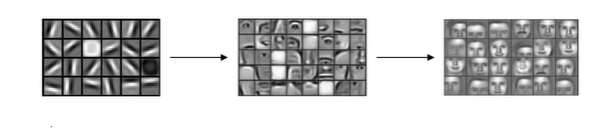
\includegraphics[width=0.85\textwidth]{Images/Edge Detection Example.png}
	\caption{Edge Detection Example}
	\label{fig:20}
\end{figure}
\FloatBarrier

\subsubsection*{Edge Detection Example}
\begin{itemize}
    \item Given an image:
    \begin{itemize}[nosep]
        \item The first step may involve detecting \textbf{vertical edges}.
        \item Similarly, \textbf{horizontal edges} can also be detected.
    \end{itemize}
\end{itemize}

To detect edges in an image:
\begin{itemize}
    \item Consider a \textbf{6x6 grayscale image} (a 6x6x1 matrix).
    \[
    \text{Image} = 
    \begin{bmatrix}
    3 & 0 & 1 & 2 & 7 & 4 \\
    1 & 5 & 8 & 9 & 3 & 1 \\
    2 & 7 & 2 & 5 & 1 & 3 \\
    0 & 1 & 3 & 1 & 7 & 8 \\
    4 & 2 & 1 & 6 & 2 & 8 \\
    2 & 4 & 5 & 2 & 3 & 9 
    \end{bmatrix}
    \]
    \item A \textbf{3x3 filter (kernel)} is defined as:
    \[
    \text{Filter} = 
    \begin{bmatrix}
    1 & 1 & 1 \\
    0 & 0 & 0 \\
    -1 & -1 & -1
    \end{bmatrix}
    \]
    \item This filter will detect \textbf{vertical edges}.
    \item The convolution operation, denoted by the symbol $*$, is applied:
    \[
    \text{Output} = \text{Image} * \text{Filter}.
    \]
\end{itemize}

In the Convolution Process:
\begin{enumerate}[nosep]
    \item The 3x3 filter is placed over a 3x3 region of the input image.
    \item The \textbf{element-wise product} of corresponding values is computed and summed to obtain a single value.
    \item The filter shifts (or slides) across the image to compute all elements of the output matrix.
    \item For a 6x6 input convolved with a 3x3 filter, the output is a \textbf{4x4 matrix}.
\end{enumerate}

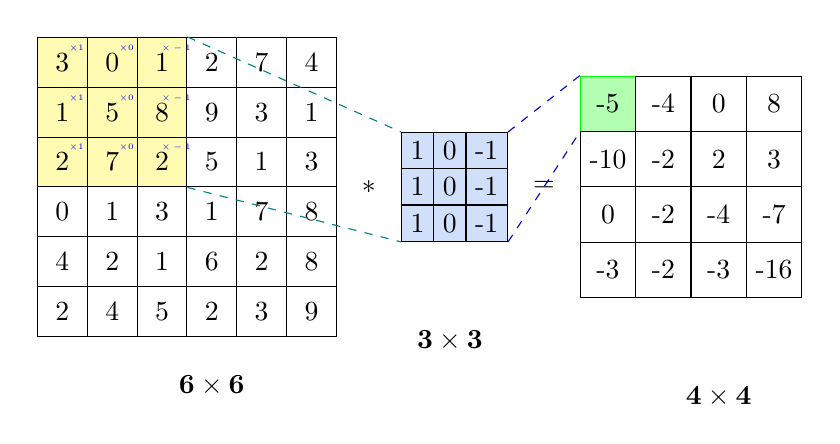
\begin{tikzpicture}[
    2d-arr/.style={matrix of nodes, row sep=-\pgflinewidth, column sep=-\pgflinewidth, nodes={draw}}
  ]

% Original image matrix
  \matrix (mtr) [2d-arr, nodes={draw, minimum width=1.8em, minimum height=1.8em, anchor=center}] {
 |[fill=yellow!30]| 3 & |[fill=yellow!30]| 0 & |[fill=yellow!30]| 1 & 2 & 7 & 4 \\
 |[fill=yellow!30]| 1 & |[fill=yellow!30]| 5 & |[fill=yellow!30]| 8 & 9 & 3 & 1 \\
 |[fill=yellow!30]| 2 & |[fill=yellow!30]| 7 & |[fill=yellow!30]| 2 & 5 & 1 & 3 \\
0 & 1 & 3 & 1 & 7 & 8 \\
4 & 2 & 1 & 6 & 2 & 8 \\
2 & 4 & 5 & 2 & 3 & 9 \\
};
\node[below=of mtr-5-4] {$\mathbf{6 \times 6}$};

% Convolution symbol
\node[right=0.2em of mtr] (conv) {$*$};

% Filter matrix
\matrix (K) [2d-arr, right=0.2em of conv, nodes={draw, fill=CornflowerBlue!30}] {
1 & 0 & -1 \\
1 & 0 & -1 \\
1 & 0 & -1 \\
};
\node[below=of K-3-2] {$\mathbf{3 \times 3}$};

% Equal sign
\node[right=0.2em of K] (eq) {$=$};

% Output matrix
\matrix (O) [2d-arr, right=0.2em of eq, column sep=-\pgflinewidth, row sep=-\pgflinewidth,
    nodes={draw, minimum width=2.0em, minimum height=2.0em, anchor=center}] {
 |[draw=green,fill=green!30]| -5 & -4 & 0 & 8 \\
-10 & -2 & 2 & 3 \\
0 & -2 & -4 & -7 \\
-3 & -2 & -3 & -16 \\
};
\node[below=of O-4-3] {$\mathbf{4 \times 4}$};

% Dashed lines to highlight one operation
\draw[dashed, teal] (mtr-1-3.north east) -- (K-1-1.north west);
\draw[dashed, teal] (mtr-3-3.south east) -- (K-3-1.south west);

\draw[dashed, blue!80!black] (K-1-3.north east) -- (O-1-1.north west);
\draw[dashed, blue!80!black] (K-3-3.south east) -- (O-1-1.south west);

% Place filter numbers on top of image matrix using foreach
\foreach \i in {1, 2,3} { % Rows of filter
    \foreach \j in {1,2,3} { % Columns of filter
        \node[font=\tiny, scale=0.6, blue, shift={(0.3,0.3)}] 
        at (mtr-\i-\j) {$\times \pgfmathparse{int(1*(\j==1) - 1*(\j==3))}\pgfmathresult$};
    }
}

\end{tikzpicture}

For the given image and filter above:
\begin{itemize}[nosep]
    \item First position: The filter is placed on the top-left 3x3 region. 
    \item Compute the element-wise product and sum:
    \[
    3 \cdot 1 + 1 \cdot 1 + 2 \cdot 1 + 0 \cdot 0 + 5 \cdot 0 + 7 \cdot 0 + 1 \cdot (-1) + 8 \cdot (-1) + 2 \cdot (-1) = -5.
    \]
    \item The value \(-5\) is placed in the top-left corner of the output matrix.
    \item Repeat this process by shifting the filter one step to the right.
\end{itemize}

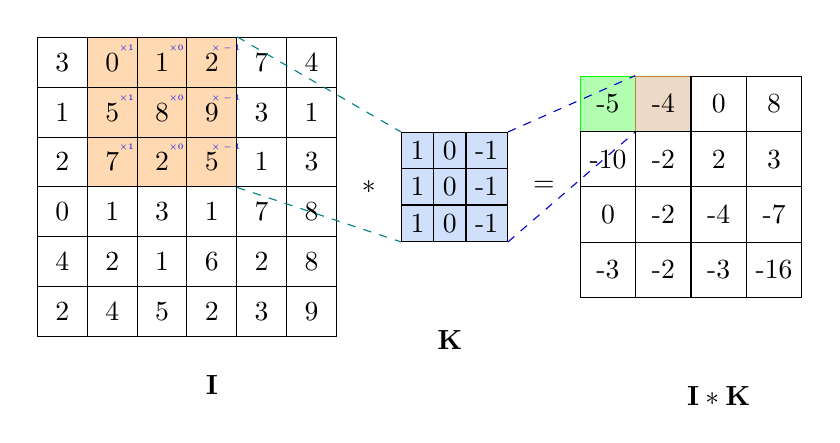
\begin{tikzpicture}[
    2d-arr/.style={matrix of nodes, row sep=-\pgflinewidth, column sep=-\pgflinewidth, nodes={draw}}
  ]

% Original image matrix
  \matrix (mtr) [2d-arr, nodes={draw, minimum width=1.8em, minimum height=1.8em, anchor=center}] {
3 & |[fill=orange!30]| 0 & |[fill=orange!30]| 1 & |[fill=orange!30]| 2 & 7 & 4 \\
1 & |[fill=orange!30]| 5 & |[fill=orange!30]| 8 & |[fill=orange!30]| 9 & 3 & 1 \\
2 & |[fill=orange!30]| 7 & |[fill=orange!30]| 2 & |[fill=orange!30]| 5 & 1 & 3 \\
0 & 1 & 3 & 1 & 7 & 8 \\
4 & 2 & 1 & 6 & 2 & 8 \\
2 & 4 & 5 & 2 & 3 & 9 \\
};
\node[below=of mtr-5-4] {$\mathbf{I}$};

% Convolution symbol
\node[right=0.2em of mtr] (conv) {$*$};

% Filter matrix
\matrix (K) [2d-arr, right=0.2em of conv, nodes={draw, fill=CornflowerBlue!30}] {
1 & 0 & -1 \\
1 & 0 & -1 \\
1 & 0 & -1 \\
};
\node[below=of K-3-2] {$\mathbf{K}$};

% Equal sign
\node[right=0.2em of K] (eq) {$=$};

% Output matrix
\matrix (O) [2d-arr, right=0.2em of eq, column sep=-\pgflinewidth, row sep=-\pgflinewidth,
    nodes={draw, minimum width=2.0em, minimum height=2.0em, anchor=center}] {
 |[draw=green, fill=green!30]| -5 &  |[draw=brown, fill=brown!30]| -4 & 0 & 8 \\
-10 & -2 & 2 & 3 \\
0 & -2 & -4 & -7 \\
-3 & -2 & -3 & -16 \\
};
\node[below=of O-4-3] {$\mathbf{I * K}$};

% Dashed lines to highlight one operation
\draw[dashed, teal] (mtr-1-4.north east) -- (K-1-1.north west);
\draw[dashed, teal] (mtr-3-4.south east) -- (K-3-1.south west);

\draw[dashed, blue!80!black] (K-1-3.north east) -- (O-1-2.north west);
\draw[dashed, blue!80!black] (K-3-3.south east) -- (O-1-2.south west);

% Place filter numbers on top of image matrix using foreach
\foreach \i in {1,2,3} { % Rows of the filter
    \foreach \j in {1,2,3} { % Columns of the filter
        % Properly compute indices with numerical expression
        \node[font=\tiny, scale=0.6, blue, shift={(0.3,0.3)}] 
        at (mtr-\the\numexpr\i\relax-\the\numexpr\j+1\relax) 
        {$\times \pgfmathparse{int(1*(\j==1) - 1*(\j==3))}\pgfmathresult$};
    }
}

\end{tikzpicture}

\begin{itemize}[nosep]
    \item At the second position, we compute the element-wise product and sum:
    \[
    0 \cdot 1 + 5 \cdot 1 + 7 \cdot 1 + 1 \cdot 0 + 8 \cdot 0 + 2 \cdot 0 + 2 \cdot (-1) + 9 \cdot (-1) + 5 \cdot (-1) = -4.
    \]
    \item The value \(-4\) is placed in the first row-second column corner of the output matrix.
    \item Repeat this process by shifting the filter one step to the right.
\end{itemize}

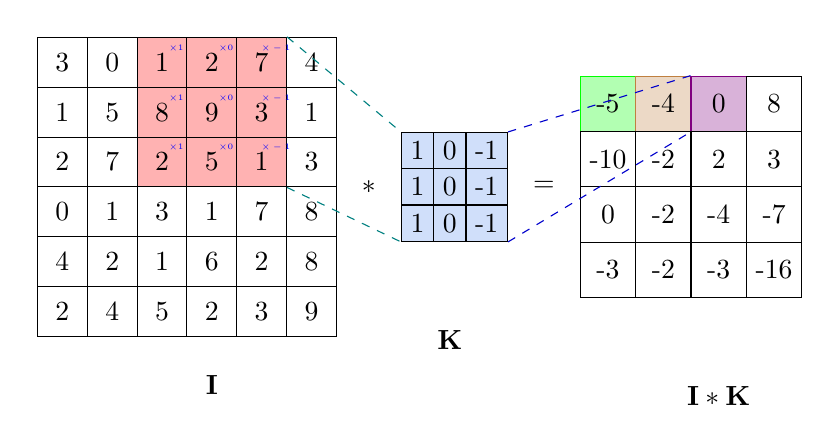
\begin{tikzpicture}[
    2d-arr/.style={matrix of nodes, row sep=-\pgflinewidth, column sep=-\pgflinewidth, nodes={draw}}
  ]

% Original image matrix
  \matrix (mtr) [2d-arr, nodes={draw, minimum width=1.8em, minimum height=1.8em, anchor=center}] {
3 & 0 & |[fill=red!30]| 1 & |[fill=red!30]| 2 &|[fill=red!30]|  7 & 4 \\
1 & 5 & |[fill=red!30]| 8 & |[fill=red!30]| 9 &|[fill=red!30]|  3 & 1 \\
2 & 7 & |[fill=red!30]| 2 & |[fill=red!30]| 5 &|[fill=red!30]|  1 & 3 \\
0 & 1 & 3 & 1 & 7 & 8 \\
4 & 2 & 1 & 6 & 2 & 8 \\
2 & 4 & 5 & 2 & 3 & 9 \\
};
\node[below=of mtr-5-4] {$\mathbf{I}$};

% Convolution symbol
\node[right=0.2em of mtr] (conv) {$*$};

% Filter matrix
\matrix (K) [2d-arr, right=0.2em of conv, nodes={draw, fill=CornflowerBlue!30}] {
1 & 0 & -1 \\
1 & 0 & -1 \\
1 & 0 & -1 \\
};
\node[below=of K-3-2] {$\mathbf{K}$};

% Equal sign
\node[right=0.2em of K] (eq) {$=$};

% Output matrix
\matrix (O) [2d-arr, right=0.2em of eq, column sep=-\pgflinewidth, row sep=-\pgflinewidth,
    nodes={draw, minimum width=2.0em, minimum height=2.0em, anchor=center}] {
 |[draw=green, fill=green!30]| -5 &  |[draw=brown, fill=brown!30]| -4 &  |[draw=violet, fill=violet!30]| 0 & 8 \\
-10 & -2 & 2 & 3 \\
0 & -2 & -4 & -7 \\
-3 & -2 & -3 & -16 \\
};
\node[below=of O-4-3] {$\mathbf{I * K}$};

% Dashed lines to highlight one operation
\draw[dashed, teal] (mtr-1-5.north east) -- (K-1-1.north west);
\draw[dashed, teal] (mtr-3-5.south east) -- (K-3-1.south west);

\draw[dashed, blue!80!black] (K-1-3.north east) -- (O-1-3.north west);
\draw[dashed, blue!80!black] (K-3-3.south east) -- (O-1-3.south west);

% Place filter numbers on top of image matrix using foreach
\foreach \i in {1,2,3} { % Rows of the filter
    \foreach \j in {1,2,3} { % Columns of the filter
        % Properly compute indices with numerical expression
        \node[font=\tiny, scale=0.6, blue, shift={(0.3,0.3)}] 
        at (mtr-\the\numexpr\i\relax-\the\numexpr\j+2\relax) 
        {$\times \pgfmathparse{int(1*(\j==1) - 1*(\j==3))}\pgfmathresult$};
    }
}

\end{tikzpicture}

\begin{itemize}[nosep]
    \item At the third position, we compute the element-wise product and sum:
    \[
    1 \cdot 1 + 8 \cdot 1 + 2 \cdot 1 + 2 \cdot 0 + 9 \cdot 0 + 5 \cdot 0 + 7 \cdot (-1) + 3 \cdot (-1) + 1 \cdot (-1) = 0.
    \]
    \item The value \(0\) is placed in the first row-third column corner of the output matrix.
    \item Repeat this process by shifting the filter one step to the right.
\end{itemize}

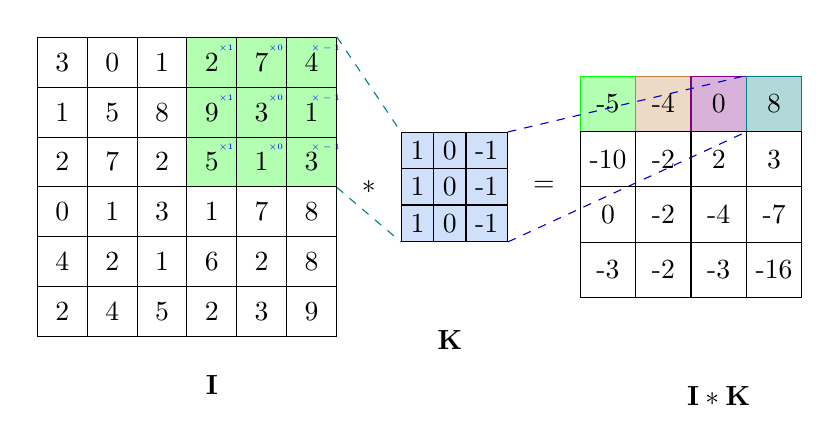
\begin{tikzpicture}[
    2d-arr/.style={matrix of nodes, row sep=-\pgflinewidth, column sep=-\pgflinewidth, nodes={draw}}
  ]

% Original image matrix
  \matrix (mtr) [2d-arr, nodes={draw, minimum width=1.8em, minimum height=1.8em, anchor=center}] {
3 & 0 &  1 & |[fill=green!30]| 2 &|[fill=green!30]|  7 &  |[fill=green!30]|4 \\
1 & 5 &  8 & |[fill=green!30]| 9 &|[fill=green!30]|  3 & |[fill=green!30]| 1 \\
2 & 7 & 2 & |[fill=green!30]| 5 &|[fill=green!30]|  1 & |[fill=green!30]| 3 \\
0 & 1 & 3 & 1 & 7 & 8 \\
4 & 2 & 1 & 6 & 2 & 8 \\
2 & 4 & 5 & 2 & 3 & 9 \\
};
\node[below=of mtr-5-4] {$\mathbf{I}$};

% Convolution symbol
\node[right=0.2em of mtr] (conv) {$*$};

% Filter matrix
\matrix (K) [2d-arr, right=0.2em of conv, nodes={draw, fill=CornflowerBlue!30}] {
1 & 0 & -1 \\
1 & 0 & -1 \\
1 & 0 & -1 \\
};
\node[below=of K-3-2] {$\mathbf{K}$};

% Equal sign
\node[right=0.2em of K] (eq) {$=$};

% Output matrix
\matrix (O) [2d-arr, right=0.2em of eq, column sep=-\pgflinewidth, row sep=-\pgflinewidth,
    nodes={draw, minimum width=2.0em, minimum height=2.0em, anchor=center}] {
 |[draw=green, fill=green!30]| -5 &  |[draw=brown, fill=brown!30]| -4 &  |[draw=violet, fill=violet!30]| 0 & |[draw=teal, fill=teal!30]|  8 \\
-10 & -2 & 2 & 3 \\
0 & -2 & -4 & -7 \\
-3 & -2 & -3 & -16 \\
};
\node[below=of O-4-3] {$\mathbf{I * K}$};

% Dashed lines to highlight one operation
\draw[dashed, teal] (mtr-1-6.north east) -- (K-1-1.north west);
\draw[dashed, teal] (mtr-3-6.south east) -- (K-3-1.south west);

\draw[dashed, blue!80!black] (K-1-3.north east) -- (O-1-4.north west);
\draw[dashed, blue!80!black] (K-3-3.south east) -- (O-1-4.south west);

% Place filter numbers on top of image matrix using foreach
\foreach \i in {1,2,3} { % Rows of the filter
    \foreach \j in {1,2,3} { % Columns of the filter
        % Properly compute indices with numerical expression
        \node[font=\tiny, scale=0.6, blue, shift={(0.3,0.3)}] 
        at (mtr-\the\numexpr\i\relax-\the\numexpr\j+3\relax) 
        {$\times \pgfmathparse{int(1*(\j==1) - 1*(\j==3))}\pgfmathresult$};
    }
}

\end{tikzpicture}

\begin{itemize}[nosep]
    \item At the fourth position, we compute the element-wise product and sum:
    \[
    2 \cdot 1 + 9 \cdot 1 + 5 \cdot 1 + 7 \cdot 0 + 3 \cdot 0 + 1 \cdot 0 + 4 \cdot (-1) + 1 \cdot (-1) + 3 \cdot (-1) = 8.
    \]
    \item The value \(8\) is placed in the first row-third column corner of the output matrix.
    \item Repeat this process by shifting the filter one step downward to the left-most 3x3 region.
\end{itemize}

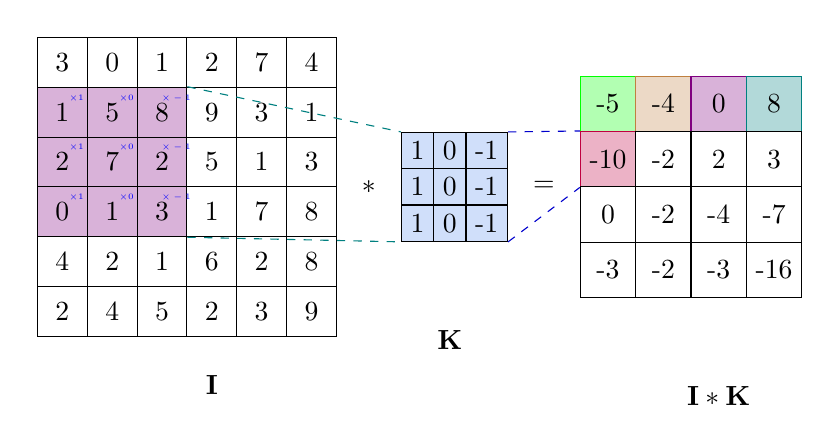
\begin{tikzpicture}[
    2d-arr/.style={matrix of nodes, row sep=-\pgflinewidth, column sep=-\pgflinewidth, nodes={draw}}
  ]

% Original image matrix
  \matrix (mtr) [2d-arr, nodes={draw, minimum width=1.8em, minimum height=1.8em, anchor=center}] {
3 & 0 &  1 & 2 & 7 & 4 \\
 |[fill=violet!30]| 1 & |[fill=violet!30]|  5 & |[fill=violet!30]|  8 & 9 & 3 & 1 \\
|[fill=violet!30]| 2 & |[fill=violet!30]| 7 &  |[fill=violet!30]| 2 & 5 & 1 & 3 \\
|[fill=violet!30]| 0 & |[fill=violet!30]| 1 & |[fill=violet!30]|  3 & 1 & 7 & 8 \\
4 & 2 & 1 & 6 & 2 & 8 \\
2 & 4 & 5 & 2 & 3 & 9 \\
};
\node[below=of mtr-5-4] {$\mathbf{I}$};

% Convolution symbol
\node[right=0.2em of mtr] (conv) {$*$};

% Filter matrix
\matrix (K) [2d-arr, right=0.2em of conv, nodes={draw, fill=CornflowerBlue!30}] {
1 & 0 & -1 \\
1 & 0 & -1 \\
1 & 0 & -1 \\
};
\node[below=of K-3-2] {$\mathbf{K}$};

% Equal sign
\node[right=0.2em of K] (eq) {$=$};

% Output matrix
\matrix (O) [2d-arr, right=0.2em of eq, column sep=-\pgflinewidth, row sep=-\pgflinewidth,
    nodes={draw, minimum width=2.0em, minimum height=2.0em, anchor=center}] {
 |[draw=green, fill=green!30]| -5 &  |[draw=brown, fill=brown!30]| -4 &  |[draw=violet, fill=violet!30]| 0 & |[draw=teal, fill=teal!30]|  8 \\
|[draw=purple, fill=purple!30]| -10 & -2 & 2 & 3 \\
0 & -2 & -4 & -7 \\
-3 & -2 & -3 & -16 \\
};
\node[below=of O-4-3] {$\mathbf{I * K}$};

% Dashed lines to highlight one operation
\draw[dashed, teal] (mtr-2-3.north east) -- (K-1-1.north west);
\draw[dashed, teal] (mtr-4-3.south east) -- (K-3-1.south west);

\draw[dashed, blue!80!black] (K-1-3.north east) -- (O-2-1.north west);
\draw[dashed, blue!80!black] (K-3-3.south east) -- (O-2-1.south west);

% Place filter numbers on top of image matrix using foreach
\foreach \i in {1,2,3} { % Rows of the filter
    \foreach \j in {1,2,3} { % Columns of the filter
        % Properly compute indices with numerical expression
        \node[font=\tiny, scale=0.6, blue, shift={(0.3,0.3)}] 
        at (mtr-\the\numexpr\i+1\relax-\the\numexpr\j\relax) 
        {$\times \pgfmathparse{int(1*(\j==1) - 1*(\j==3))}\pgfmathresult$};
    }
}

\end{tikzpicture}

\begin{itemize}[nosep]
    \item At the fifth position, we compute the element-wise product and sum:
    \[
    1 \cdot 1 + 2 \cdot 1 + 0 \cdot 1 + 5 \cdot 0 + 7 \cdot 0 + 1 \cdot 0 + 8 \cdot (-1) + 2 \cdot (-1) + 3 \cdot (-1) = -10.
    \]
    \item The value \(-10\) is placed in the second row-first column corner of the output matrix.
    \item Repeat this process by shifting the filter one step to the left and so on.
\end{itemize}

Consider a simple 6x6 image in  \textbf{Fig. \ref{fig:21}} where:
    \begin{itemize}[nosep]
        \item The left half has pixel values of 10.
        \item The right half has pixel values of 0.
        \item Plotting as an image gives a left half that denotes brighter pixel intensive values and the right half gives you darker pixel intensive values
    \end{itemize}
The 3x3 filter detects the \textbf{vertical edge} separating the two halves:
    \[
    \text{Left: Bright pixels, Middle: Zero, Right: Dark pixels}.
    \]
The output matrix will highlight the edge as a \textbf{bright vertical line}.

% Figure 21
\begin{figure}[h]
	\centering
	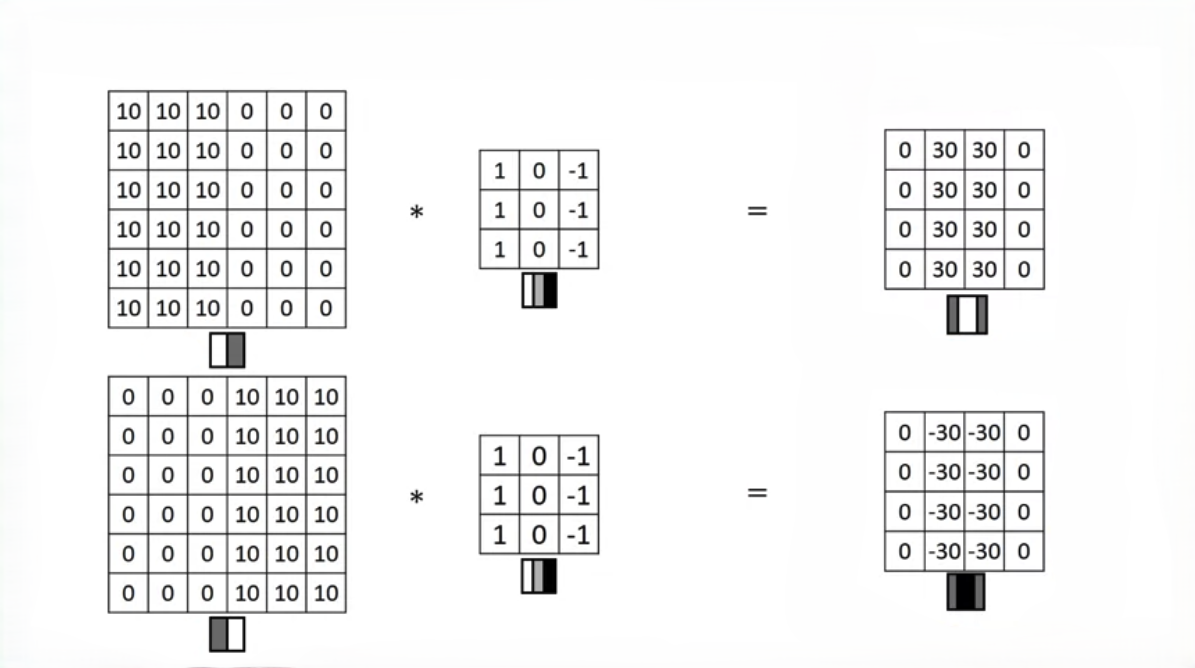
\includegraphics[width=0.85\textwidth]{Images/Vertical Edge Detection Examples.png}
	\caption{Vertical Edge Detection Examples}
	\label{fig:21}
\end{figure}
\FloatBarrier

\subsubsection*{Vertical and Horizontal Edge Detection Example}
There are different edge detectors, such as vertical and horizontal filters shown in \textbf{Fig. \ref{fig:22}}. Other types of filter includes Sobel and Scharr filters. A vertical edge occurs where there are bright pixels on the left and dark pixels on the right. The convolution operation captures this pattern effectively:
    \begin{itemize}[nosep]
        \item Bright pixels on the left produce positive values.
        \item Dark pixels on the right produce negative values.
        \item Positive and negative edge detection (light-to-dark vs.~dark-to-light transitions).
    \end{itemize}

% Figure 22
\begin{figure}[h]
	\centering
	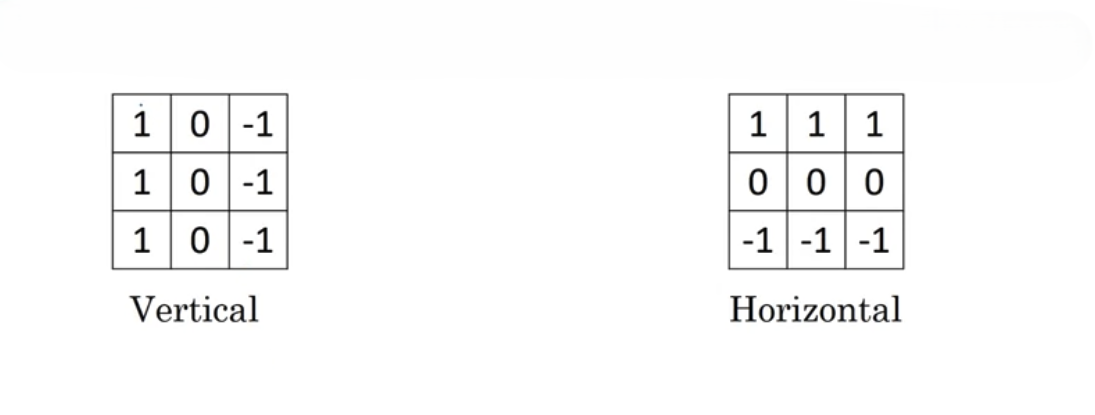
\includegraphics[width=0.65\textwidth]{Images/Vertical and Horizontal Edge Detection.png}
	\caption{Vertical and Horizontal Edge Detection}
	\label{fig:22}
\end{figure}
\FloatBarrier

\subsubsection{Vertical Edge Detection Example}
\begin{itemize}[nosep]
    \item A vertical edge detection filter detects transitions from bright to dark regions (light-to-dark).
    \item If the image colors are flipped (dark-to-light), the output is a negative value.
    \item Taking the absolute value of the output removes the distinction between edge direction.
\end{itemize}

\subsubsection{Horizontal Edge Detection}
\begin{itemize}[nosep]
    \item A horizontal edge detection filter detects transitions between bright pixels on top and dark pixels below.
    \item Example:
    \begin{itemize}
        \item Positive edge: bright pixels on top and dark on the bottom.
        \item Negative edge: dark pixels on top and bright on the bottom.
    \end{itemize}
    \item Intermediate values occur due to blending positive and negative edges in small images (e.g., $6 \times 6$).
\end{itemize}
The \textbf{convolution operation} provides a systematic way to detect edges in an image.Vertical and horizontal edge detection are foundational concepts for building Convolutional Neural Networks (CNNs).

\subsubsection{Sobel and Scharr Filters}
\begin{itemize}
    \item The \textbf{Sobel filter} enhances robustness by emphasizing the center row.  It puts a little bit more weight to the central row, the central pixel, and this makes it maybe a little bit more robust.
    \[
    \begin{bmatrix}
    1 & 0 & -1 \\
    2 & 0 & -2 \\
    1 & 0 & -1
    \end{bmatrix}
    \]
    \item The \textbf{Scharr filter} uses different weights for improved performance:
    \[
    \begin{bmatrix}
    3 & 0 & -3 \\
    10 & 0 & -10 \\
    3 & 0 & -3
    \end{bmatrix}
    \]
    \item Flipping these filters by $90^\circ$ produces horizontal edge detectors.
\end{itemize}

\subsubsection*{Learning Filters with Backpropagation}
\begin{itemize}
    \item Instead of hand-coding filters, deep learning allows learning filters as parameters through backpropagation.
    \item The $3 \times 3$ filter values are treated as parameters to optimize.
    \[
    \begin{bmatrix}
    w_1 & w_2 & w_3 \\
    w_4 & w_5 & w_6 \\
    w_7 & w_8 & w_9
    \end{bmatrix}
    \]
    \item Neural networks can learn:
    \begin{itemize}
        \item Vertical, horizontal, and diagonal edges.
        \item Complex features beyond predefined filters.
    \end{itemize}
    \item Example: Neural networks can learn edges at arbitrary angles (e.g., $45^\circ$, $70^\circ$).
\end{itemize}
The convolution operation enables backpropagation to learn any filter that detects relevant features in an image, such as edges, by applying it across the entire image.

% ---------------- Padding ----------------------%
\subsection{Padding in Convolutional Neural Networks}

Padding is used in convolutional operations to address two main problems:
\begin{enumerate}
    \item Shrinking of the image size after each convolution.
    \item Loss of information from the edges of the image.
\end{enumerate}

% Figure 23
\begin{figure}[h]
	\centering
	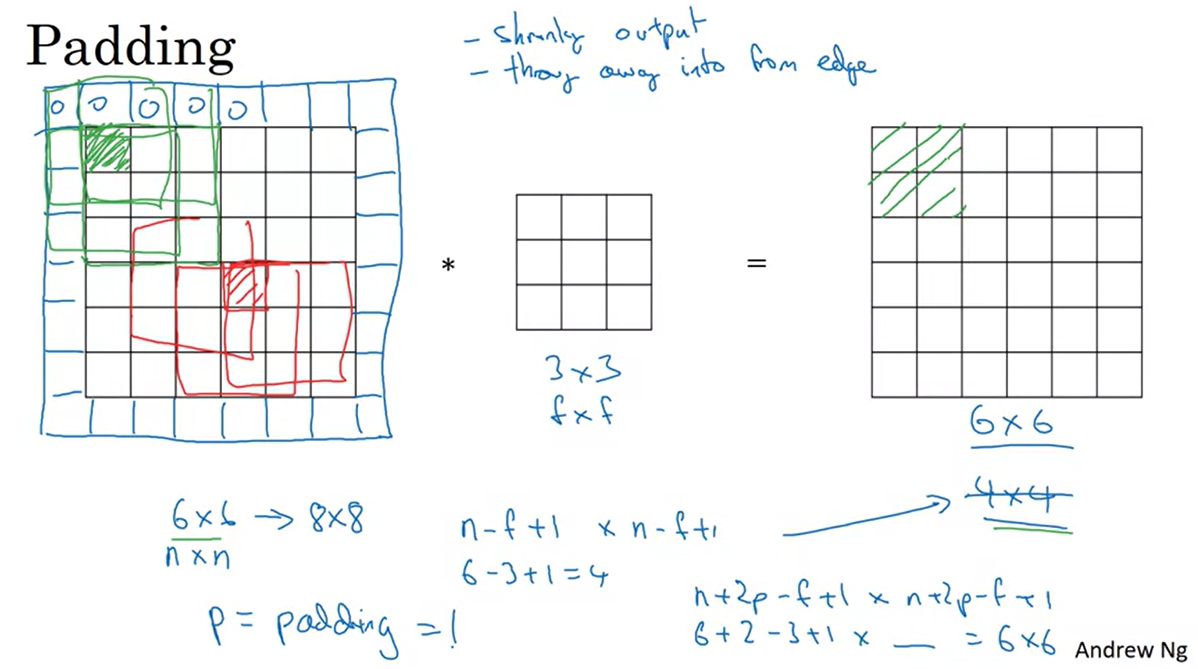
\includegraphics[width=0.85\textwidth]{Images/Padding.png}
	\caption{Padding in Convolutional Neural Networks}
	\label{fig:23}
\end{figure}
\FloatBarrier

\subsubsection*{Convolution Without Padding}
When convolving an \(n \times n\) image with an \(f \times f\) filter, the output size is:
\[
\text{Output Size} = (n - f + 1) \times (n - f + 1).
\]
A \(6 \times 6\) image convolved with a \(3 \times 3\) filter results in a \(4 \times 4\) output.

The downsides of Convolution without padding is that:
\begin{enumerate}[nosep]
    \item The image size reduces with each convolution, which is problematic in deep networks.
    \item Edge pixels are used less frequently in the output, leading to information loss at the boundaries.
\end{enumerate}

To avoid this, we add padding to the image. Padding involves adding a border of pixels (typically zero-valued) around the image to preserve its size after convolution.

The formula for the output size with padding is:
\[
\text{Output Size} = (n + 2p - f + 1) \times (n + 2p - f + 1),
\]
where \(p\) is the padding amount.

\textbf{Example:}
\begin{itemize}[nosep]
    \item A \(6 \times 6\) image padded with \(p = 1\) becomes an \(8 \times 8\) image.
    \item Convolving this \(8 \times 8\) image with a \(3 \times 3\) filter results in a \(6 \times 6\) output, preserving the original image size.
\end{itemize}

\subsubsection*{Types of Convolutions}
\begin{enumerate}
    \item \textbf{Valid Convolution:} No padding (\(p = 0\)).
    \[
    \text{Output Size} = (n - f + 1) \times (n - f + 1).
    \]

    \item \textbf{Same Convolution:} Padding is applied to ensure the output size is the same as the input size. The padding is calculated as:
    \[
    p = \frac{f - 1}{2}.
    \]
    \textbf{Examples:}
    \begin{itemize}[nosep]
        \item For a \(3 \times 3\) filter (\(f = 3\)), \(p = 1\).
        \item For a \(5 \times 5\) filter (\(f = 5\)), \(p = 2\).
    \end{itemize}
\end{enumerate}

\subsubsection*{Why Filters are Usually Odd-Sized}
Odd-sized filters (e.g., \(3 \times 3\), \(5 \times 5\)) are preferred because:
\begin{enumerate}[nosep]
    \item They ensure symmetric padding, avoiding uneven padding on different sides.
    \item They have a central pixel, making it easier to define the filter’s position.
\end{enumerate}

\subsubsection*{Padding in Practice}
To specify padding for your convolution operation, you can:
\begin{enumerate}
    \item Explicitly set the padding value (\(p\)).
    \item Use predefined options:
    \begin{itemize}
        \item \textbf{Valid Convolution:} \(p = 0\).
        \item \textbf{Same Convolution:} Automatically pads to maintain input size.
    \end{itemize}
\end{enumerate}

Odd-sized filters (e.g., \(3 \times 3\), \(5 \times 5\)) are recommended for compatibility with common conventions in computer vision.

% ---------------- Convolution ----------------------%
\subsection{Convolution}
\subsection*{Strided Convolutions}
Stride convolutions are a fundamental concept in convolutional neural networks (CNNs). The stride determines how the convolutional filter moves across the input image during the convolution operation.

\textbf{Example with a Stride of 2} \\
Suppose you have a $7 \times 7$ image and a $3 \times 3$ filter. Instead of shifting the filter one step at a time (as in standard convolution), you move it \textbf{two steps} at a time (stride $s = 2$).

\begin{enumerate}
    \item Perform the element-wise product in the upper-left $3 \times 3$ region of the image, sum the values, and store the result (e.g., $91$).
    \item Move the filter \textbf{two steps to the right} (instead of one). Compute the next output (e.g., $100$).
    \item Repeat this process across the entire row.
    \item When moving to the next row, \textbf{step down by two rows} instead of one and repeat the process.
\end{enumerate}

\textbf{Result:} Convolving a $7 \times 7$ image with a $3 \times 3$ filter using a stride of $2$ results in a $3 \times 3$ output.

\subsubsection*{Output Size Formula}
For an input image of size $n \times n$, a filter of size $f \times f$, padding $p$, and stride $s$, the output dimensions are given by:
\[
\text{Output Size} = \left\lfloor \frac{n + 2p - f}{s} + 1 \right\rfloor
\]
where $\lfloor \cdot \rfloor$ denotes the floor function (rounding down to the nearest integer).

\begin{tikzpicture}[
    2d-arr/.style={matrix of nodes, row sep=-\pgflinewidth, column sep=-\pgflinewidth, nodes={draw}}
  ]

% Original image matrix
  \matrix (mtr) [2d-arr, nodes={draw, minimum width=2.0em, minimum height=2.0em, anchor=center}] {
 |[fill=yellow!30]| 2 & |[fill=yellow!30]| 3 & |[fill=yellow!30]| 7 & 4 & 6 & 2 & 9  \\
 |[fill=yellow!30]| 6 & |[fill=yellow!30]| 6 & |[fill=yellow!30]| 9 & 8 & 7 & 4 & 3  \\
 |[fill=yellow!30]| 3 & |[fill=yellow!30]| 4 & |[fill=yellow!30]| 8 & 3 & 8 & 9 & 7 \\
7 & 8 & 3 & 6 & 6 & 3 & 4 \\
4 & 2 & 1 & 8 & 3 & 4 & 6 \\
3 & 2 & 4 & 1 & 9 & 8 & 3 \\
0 & 1 & 3 & 9 & 2 & 1 & 4 \\
};
\node[below=4.0em of mtr-5-4] {$\mathbf{7 \times 7}$};

% Convolution symbol
\node[right=0.2em of mtr] (conv) {$*$};

% Filter matrix
\matrix (K) [2d-arr, right=0.2em of conv, column sep=-\pgflinewidth, row sep=-\pgflinewidth, 
	nodes={draw, minimum width=2.0em, minimum height=2.0em, anchor=center, fill=CornflowerBlue!30}] {
1 & 0 & -1 \\
1 & 0 & -1 \\
1 & 0 & -1 \\
};
\node[below=0.2em of K-3-2] {$\mathbf{3 \times 3}$};

% Equal sign
\node[right=0.2em of K] (eq) {$=$};

% Output matrix
\matrix (O) [2d-arr, right=0.2em of eq, column sep=-\pgflinewidth, row sep=-\pgflinewidth,
    nodes={draw, minimum width=2.0em, minimum height=2.0em, anchor=center}] {
 |[draw=green,fill=green!30]| -13 & 3 & 2 \\
2 & -5 & 0 \\
-1 & -6 & 1 \\
};
\node[below=-1.0em of O-4-4] {$\mathbf{3 \times 3}$};

% Dashed lines to highlight one operation
\draw[dashed, teal] (mtr-1-3.north east) -- (K-1-1.north west);
\draw[dashed, teal] (mtr-3-3.south east) -- (K-3-1.south west);

\draw[dashed, blue!80!black] (K-1-3.north east) -- (O-1-1.north west);
\draw[dashed, blue!80!black] (K-3-3.south east) -- (O-1-1.south west);

% Place filter numbers on top of image matrix using foreach
\foreach \i in {1, 2,3} { % Rows of filter
    \foreach \j in {1,2,3} { % Columns of filter
        \node[font=\tiny, scale=0.6, blue, shift={(0.3,0.3)}] 
        at (mtr-\i-\j) {$\times \pgfmathparse{int(1*(\j==1) - 1*(\j==3))}\pgfmathresult$};
    }
}

\end{tikzpicture}

\begin{tikzpicture}[
    2d-arr/.style={matrix of nodes, row sep=-\pgflinewidth, column sep=-\pgflinewidth, nodes={draw}}
  ]

% Original image matrix
  \matrix (mtr) [2d-arr, nodes={draw, minimum width=2.0em, minimum height=2.0em, anchor=center}] {
 2 &  3 & |[fill=orange!30]| 7 & |[fill=orange!30]| 4 & |[fill=orange!30]| 6 & 2 & 9  \\
  6 & 6 & |[fill=orange!30]| 9 & |[fill=orange!30]| 8 & |[fill=orange!30]| 7 & 4 & 3  \\
 3 & 4 & |[fill=orange!30]| 8 & |[fill=orange!30]| 3 & |[fill=orange!30]| 8 & 9 & 7 \\
7 & 8 & 3 & 6 & 6 & 3 & 4 \\
4 & 2 & 1 & 8 & 3 & 4 & 6 \\
3 & 2 & 4 & 1 & 9 & 8 & 3 \\
0 & 1 & 3 & 9 & 2 & 1 & 4 \\
};
\node[below=4.0em of mtr-5-4] {$\mathbf{7 \times 7}$};

% Convolution symbol
\node[right=0.2em of mtr] (conv) {$*$};

% Filter matrix
\matrix (K) [2d-arr, right=0.2em of conv, column sep=-\pgflinewidth, row sep=-\pgflinewidth, 
	nodes={draw, minimum width=2.0em, minimum height=2.0em, anchor=center, fill=CornflowerBlue!30}] {
1 & 0 & -1 \\
1 & 0 & -1 \\
1 & 0 & -1 \\
};
\node[below=0.2em of K-3-2] {$\mathbf{3 \times 3}$};

% Equal sign
\node[right=0.2em of K] (eq) {$=$};

% Output matrix
\matrix (O) [2d-arr, right=0.2em of eq, column sep=-\pgflinewidth, row sep=-\pgflinewidth,
    nodes={draw, minimum width=2.0em, minimum height=2.0em, anchor=center}] {
 |[draw=green,fill=green!30]| -13 &  |[draw=brown, fill=brown!30]| 3 & 2 \\
2 & -5 & 0 \\
-1 & -6 & 1 \\
};
\node[below=-1.0em of O-4-4] {$\mathbf{3 \times 3}$};

% Dashed lines to highlight one operation
\draw[dashed, teal] (mtr-1-5.north east) -- (K-1-1.north west);
\draw[dashed, teal] (mtr-3-5.south east) -- (K-3-1.south west);

\draw[dashed, blue!80!black] (K-1-3.north east) -- (O-1-2.north west);
\draw[dashed, blue!80!black] (K-3-3.south east) -- (O-1-2.south west);

% Place filter numbers on top of image matrix using foreach
\foreach \i in {1,2,3} { % Rows of the filter
    \foreach \j in {1,2,3} { % Columns of the filter
        % Properly compute indices with numerical expression
        \node[font=\tiny, scale=0.6, blue, shift={(0.3,0.3)}] 
        at (mtr-\the\numexpr\i\relax-\the\numexpr\j+2\relax) 
        {$\times \pgfmathparse{int(1*(\j==1) - 1*(\j==3))}\pgfmathresult$};
    }
}

\end{tikzpicture}

\begin{tikzpicture}[
    2d-arr/.style={matrix of nodes, row sep=-\pgflinewidth, column sep=-\pgflinewidth, nodes={draw}}
  ]

% Original image matrix
  \matrix (mtr) [2d-arr, nodes={draw, minimum width=2.0em, minimum height=2.0em, anchor=center}] {
 2 &  3 &  7 & 4 & |[fill=red!30]| 6 & |[fill=red!30]| 2 & |[fill=red!30]| 9  \\
  6 & 6 & 9 & 8 & |[fill=red!30]| 7 & |[fill=red!30]| 4 & |[fill=red!30]| 3  \\
 3 & 4 & 8 & 3 & |[fill=red!30]|  8 & |[fill=red!30]| 9 & |[fill=red!30]| 7 \\
7 & 8 & 3 & 6 & 6 & 3 & 4 \\
4 & 2 & 1 & 8 & 3 & 4 & 6 \\
3 & 2 & 4 & 1 & 9 & 8 & 3 \\
0 & 1 & 3 & 9 & 2 & 1 & 4 \\
};
\node[below=4.0em of mtr-5-4] {$\mathbf{7 \times 7}$};

% Convolution symbol
\node[right=0.2em of mtr] (conv) {$*$};

% Filter matrix
\matrix (K) [2d-arr, right=0.2em of conv, column sep=-\pgflinewidth, row sep=-\pgflinewidth, 
	nodes={draw, minimum width=2.0em, minimum height=2.0em, anchor=center, fill=CornflowerBlue!30}] {
1 & 0 & -1 \\
1 & 0 & -1 \\
1 & 0 & -1 \\
};
\node[below=0.2em of K-3-2] {$\mathbf{3 \times 3}$};

% Equal sign
\node[right=0.2em of K] (eq) {$=$};

% Output matrix
\matrix (O) [2d-arr, right=0.2em of eq, column sep=-\pgflinewidth, row sep=-\pgflinewidth,
    nodes={draw, minimum width=2.0em, minimum height=2.0em, anchor=center}] {
 |[draw=green,fill=green!30]| -13 &  |[draw=brown, fill=brown!30]| 3 & |[draw=violet, fill=violet!30]| 2 \\
2 & -5 & 0 \\
-1 & -6 & 1 \\
};
\node[below=-1.0em of O-4-4] {$\mathbf{3 \times 3}$};

% Dashed lines to highlight one operation
\draw[dashed, teal] (mtr-1-7.north east) -- (K-1-1.north west);
\draw[dashed, teal] (mtr-3-7.south east) -- (K-3-1.south west);

\draw[dashed, blue!80!black] (K-1-3.north east) -- (O-1-3.north west);
\draw[dashed, blue!80!black] (K-3-3.south east) -- (O-1-3.south west);

% Place filter numbers on top of image matrix using foreach
\foreach \i in {1,2,3} { % Rows of the filter
    \foreach \j in {1,2,3} { % Columns of the filter
        % Properly compute indices with numerical expression
        \node[font=\tiny, scale=0.6, blue, shift={(0.3,0.3)}] 
        at (mtr-\the\numexpr\i\relax-\the\numexpr\j+4\relax) 
        {$\times \pgfmathparse{int(1*(\j==1) - 1*(\j==3))}\pgfmathresult$};
    }
}

\end{tikzpicture}

\begin{tikzpicture}[
    2d-arr/.style={matrix of nodes, row sep=-\pgflinewidth, column sep=-\pgflinewidth, nodes={draw}}
  ]

% Original image matrix
  \matrix (mtr) [2d-arr, nodes={draw, minimum width=2.0em, minimum height=2.0em, anchor=center}] {
 2 &  3 & 7 & 4 & 6 & 2 & 9  \\
 6 & 6 & 9 & 8 &  7 & 4 & 3  \\
|[fill=violet!30]| 3 & |[fill=violet!30]| 4 & |[fill=violet!30]| 8 & 3 &  8 & 9 & 7 \\
|[fill=violet!30]| 7 & |[fill=violet!30]| 8 & |[fill=violet!30]| 3 & 6 & 6 & 3 & 4 \\
|[fill=violet!30]| 4 & |[fill=violet!30]| 2 & |[fill=violet!30]| 1 & 8 & 3 & 4 & 6 \\
3 & 2 & 4 & 1 & 9 & 8 & 3 \\
0 & 1 & 3 & 9 & 2 & 1 & 4 \\
};
\node[below=4.0em of mtr-5-4] {$\mathbf{7 \times 7}$};

% Convolution symbol
\node[right=0.2em of mtr] (conv) {$*$};

% Filter matrix
\matrix (K) [2d-arr, right=0.2em of conv, column sep=-\pgflinewidth, row sep=-\pgflinewidth, 
	nodes={draw, minimum width=2.0em, minimum height=2.0em, anchor=center, fill=CornflowerBlue!30}] {
1 & 0 & -1 \\
1 & 0 & -1 \\
1 & 0 & -1 \\
};
\node[below=0.2em of K-3-2] {$\mathbf{3 \times 3}$};

% Equal sign
\node[right=0.2em of K] (eq) {$=$};

% Output matrix
\matrix (O) [2d-arr, right=0.2em of eq, column sep=-\pgflinewidth, row sep=-\pgflinewidth,
    nodes={draw, minimum width=2.0em, minimum height=2.0em, anchor=center}] {
|[draw=green,fill=green!30]| -13 &  |[draw=brown, fill=brown!30]| 3 & 2 \\
|[draw=purple, fill=purple!30]| 2 & -5 & 0 \\
-1 & -6 & 1 \\
};
\node[below=-1.0em of O-4-4] {$\mathbf{3 \times 3}$};

% Dashed lines to highlight one operation
\draw[dashed, teal] (mtr-3-3.north east) -- (K-1-1.north west);
\draw[dashed, teal] (mtr-5-3.south east) -- (K-3-1.south west);

\draw[dashed, blue!80!black] (K-1-3.north east) -- (O-2-1.north west);
\draw[dashed, blue!80!black] (K-3-3.south east) -- (O-2-1.south west);

% Place filter numbers on top of image matrix using foreach
\foreach \i in {1,2,3} { % Rows of the filter
    \foreach \j in {1,2,3} { % Columns of the filter
        % Properly compute indices with numerical expression
        \node[font=\tiny, scale=0.6, blue, shift={(0.3,0.3)}] 
        at (mtr-\the\numexpr\i+2\relax-\the\numexpr\j\relax) 
        {$\times \pgfmathparse{int(1*(\j==1) - 1*(\j==3))}\pgfmathresult$};
    }
}

\end{tikzpicture}

\subsubsection*{Example Calculation}
\begin{itemize}[nosep]
    \item Input size: $7 \times 7$
    \item Filter size: $3 \times 3$
    \item Padding: $p = 0$
    \item Stride: $s = 2$
\end{itemize}

\[
\text{Output Size} = \left\lfloor \frac{7 + 2(0) - 3}{2} + 1 \right\rfloor = \left\lfloor \frac{4}{2} + 1 \right\rfloor = \left\lfloor 3 \right\rfloor = 3
\]

It is important to note that:
\begin{enumerate}
    \item If the output size formula results in a fraction, it is rounded down using the floor function.
    \item A convolution is only performed if the filter lies entirely within the input image (or input + padding). If part of the filter extends beyond the image, that position is skipped.
\end{enumerate}

\subsubsection*{Convolutions vs. Cross-Correlation}
\begin{itemize}
    \item In traditional mathematics, convolutions involve flipping the filter both horizontally and vertically before performing the element-wise product and summation.
    \item In deep learning, this flipping step is typically skipped. The operation performed is technically \textbf{cross-correlation}, but it is conventionally referred to as \textbf{convolution}.
\end{itemize}

Omitting the flipping simplifies implementation and does not impact neural network performance. This distinction does not affect the understanding or implementation of CNNs.

In summary:
\begin{itemize}[nosep]
    \item Stride controls the step size of the filter’s movement across the input.
    \item The output size depends on the input dimensions, filter size, padding, and stride.
    \item In deep learning, convolution is implemented without flipping the filter, which is technically cross-correlation but conventionally referred to as convolution.
\end{itemize}

% ---------------- Convolutions Over Volume ----------------------%
\subsection{Convolutions Over Volume}
You've seen how convolutions work over 2D images. Now, let's explore how to implement convolutions over three-dimensional volumes. 

\subsubsection*{Example: Convolution on an RGB Image}

Suppose you want to detect features in an RGB image. An RGB image can be represented as a $6 \times 6 \times 3$ volume, where:
\begin{itemize}[nosep]
    \item The first dimension ($6$) is the \textbf{height}.
    \item The second dimension ($6$) is the \textbf{width}.
    \item The third dimension ($3$) is the \textbf{number of channels} (red, green, and blue).
\end{itemize}

Instead of convolving this with a $3 \times 3$ filter as done with grayscale images, we now use a 3D filter of size $3 \times 3 \times 3$. The filter also has three layers corresponding to the red, green, and blue channels. 

% Figure 24
\begin{figure}[h]
	\centering
	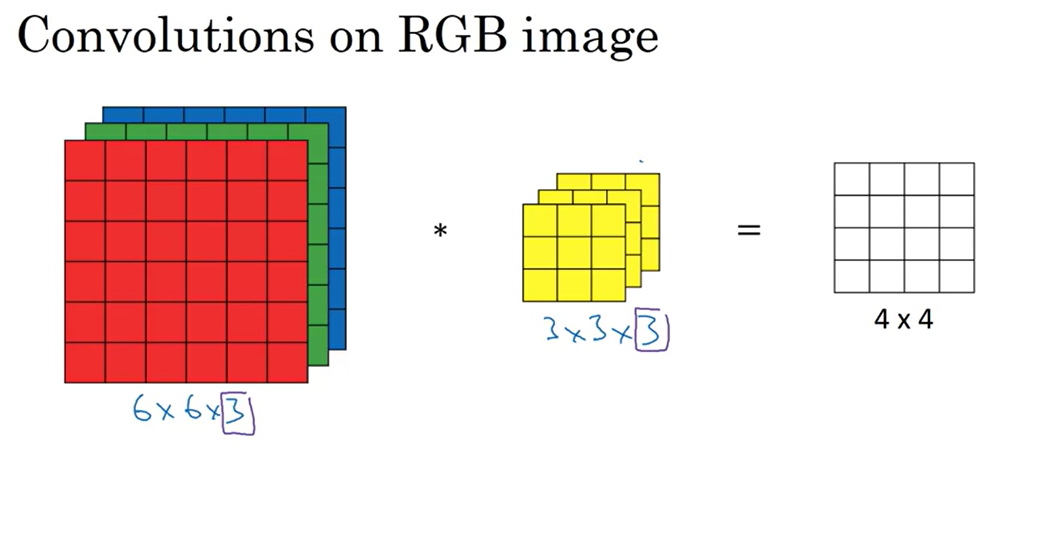
\includegraphics[width=0.85\textwidth]{Images/Convolution on 3D Image.png}
	\caption{Convolution on 3D Image}
	\label{fig:24}
\end{figure}
\FloatBarrier

\textbf{Key Condition:} The number of channels in the filter must match the number of channels in the input image.

\subsubsection*{Convolution Operation}
To compute the output of a $6 \times 6 \times 3$ input convolved with a $3 \times 3 \times 3$ filter:
\begin{enumerate}
    \item Place the $3 \times 3 \times 3$ filter at the upper-left corner of the input volume.
    \item Multiply each of the $27$ parameters of the filter with the corresponding numbers in the input volume covered by the filter.
    \item Add up the $27$ multiplications to compute a single output value.
    \item Slide the filter to the next position (e.g., one step to the right) and repeat the operation.
    \item Continue until all positions are covered.
\end{enumerate}

The result of this operation is a $4 \times 4 \times 1$ output volume (assuming a stride of $1$ and no padding). Notice that the output now has only one channel because a single filter was applied.
 
% Figure 25
\begin{figure}[h]
	\centering
	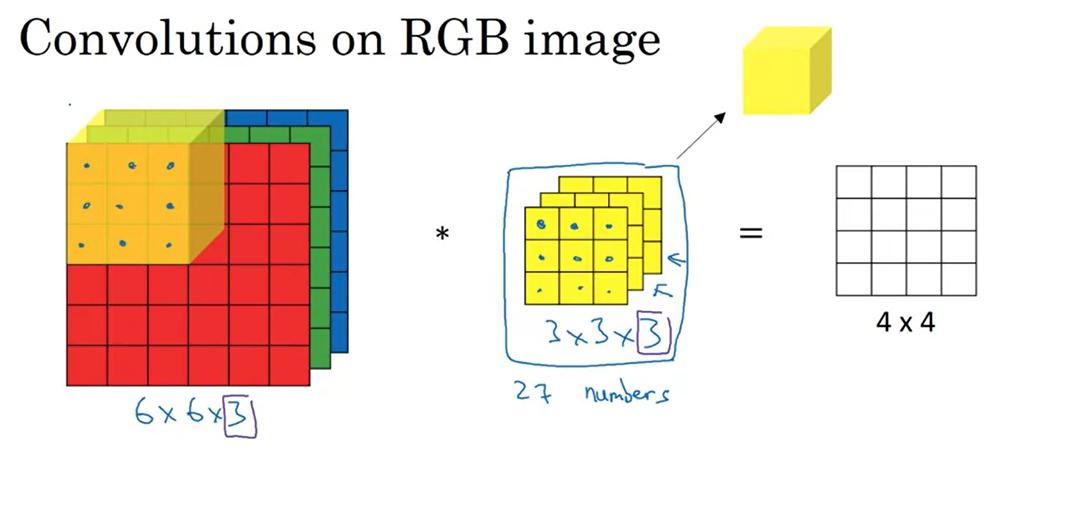
\includegraphics[width=0.85\textwidth]{Images/Convolution Operation.png}
	\caption{Convolution Operation}
	\label{fig:25}
\end{figure}
\FloatBarrier

\subsection*{Using Multiple Filters}
If you want to detect multiple features (e.g., vertical edges, horizontal edges, 45-degree edges), you can use multiple filters simultaneously:
\begin{itemize}
    \item Each filter produces a separate $4 \times 4$ output.
    \item These outputs are stacked together to form a $4 \times 4 \times N$ volume, where $N$ is the number of filters.
\end{itemize}

For example, applying two filters to a $6 \times 6 \times 3$ input results in a $4 \times 4 \times 2$ output.

% Figure 26
\begin{figure}[h]
	\centering
	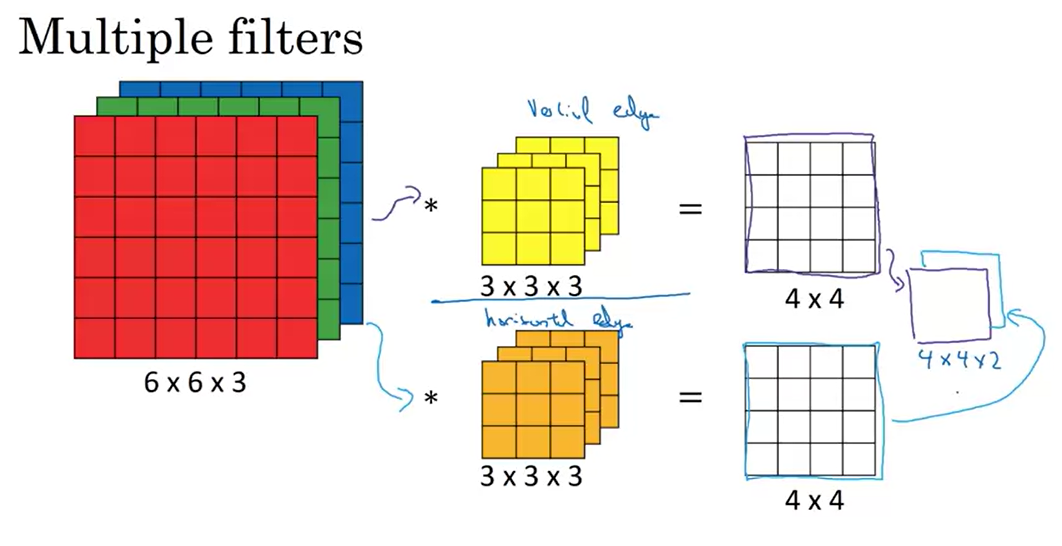
\includegraphics[width=0.85\textwidth]{Images/Multiple Filters.png}
	\caption{Multiple Filters}
	\label{fig:26}
\end{figure}
\FloatBarrier

\subsubsection*{Summary of Dimensions of Convolution Output}
Given an input of size $n \times n \times n_C$ (height, width, channels) and a filter of size $f \times f \times n_C$, the output dimensions are:
\[
(n - f + 1) \times (n - f + 1) \times n_C'
\]
where $n_C'$ is the number of filters applied.

\textbf{Notes:}
\begin{itemize}
    \item If stride or padding is used, the formula for the output size is adjusted accordingly.
    \item The number of channels in the output is equal to the number of filters.
\end{itemize}

\subsubsection*{Applications and Notation}
\begin{itemize}[nosep]
    \item Convolutions over volumes enable feature detection in multi-channel images (e.g., RGB).
    \item You can detect multiple features simultaneously by using multiple filters.
    \item The output of the convolution will have as many channels as the number of filters.
    \item The term \textbf{channels} is commonly used to refer to the third dimension of the input or output volume. Some literature refers to this as the \textbf{depth}, but this term can be ambiguous.
\end{itemize}

Now that you understand convolutions over volumes, you're ready to implement one layer of a convolutional neural network.

% ---------------- Building One Layer of a Convolutional Neural Network ----------------------%
\subsection{Building One Layer of a Convolutional Neural Network}
To build one layer of a convolutional neural network, we start by convolving a 3D volume with filters. For example:
\begin{itemize}[nosep]
    \item Convolve the input with two filters to produce two 4x4 outputs.
    \item Add biases to these outputs. Each bias is a single number added to all 16 elements in the output matrix using broadcasting.
    \item Apply a non-linearity (e.g., ReLU) to these outputs.
\end{itemize}

Finally, stack the resulting matrices to form a 4x4x2 output. This operation represents one layer of a convolutional neural network.

% Figure 27
\begin{figure}[h]
	\centering
	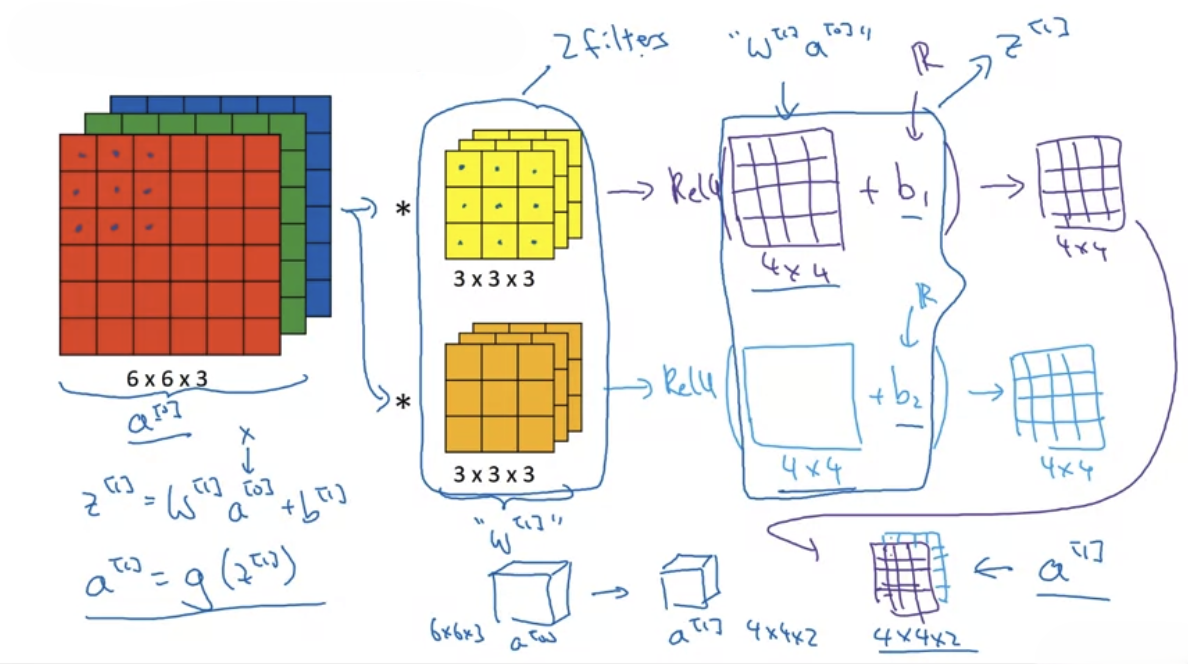
\includegraphics[width=\textwidth]{Images/One Layer of a CNN.png}
	\caption{One Layer of a CNN}
	\label{fig:27}
\end{figure}
\FloatBarrier

\subsubsection*{Relation to Traditional Neural Networks}
In a traditional neural network, forward propagation involves:
\[
z^{[1]} = W^{[1]} \cdot a^{[0]} + b^{[1]},
\]
where \( a^{[0]} = x \). Similarly, in a convolutional neural network:
\begin{itemize}[nosep]
    \item The filters play a role similar to \( W^{[1]} \).
    \item The output of the convolution operation corresponds to \( W^{[1]} \cdot a^{[0]} \).
    \item Adding biases corresponds to adding \( b^{[1]} \).
    \item Applying the non-linearity corresponds to obtaining activations \( a^{[1]} \).
\end{itemize}
Thus, the convolution operation can be viewed as applying a linear transformation followed by a non-linearity.

\subsubsection*{Number of Parameters in a Convolutional Layer}
Consider an example with 10 filters, each of size \( 3 \times 3 \times 3 \):
\begin{itemize}
    \item Each filter has \( 3 \times 3 \times 3 = 27 \) parameters, plus 1 bias, resulting in \( 28 \) parameters per filter.
    \item With 10 filters, the total number of parameters is:
    \[
    28 \times 10 = 280.
    \]
\end{itemize}

This fixed number of parameters makes convolutional neural networks less prone to overfitting, regardless of the input image size.

\subsubsection*{Convolutional Layer Notation}
To describe one convolutional layer \( l \):
\begin{itemize}[nosep]
    \item \( f^{[l]} \): Filter size (e.g., \( f \times f \)).
    \item \( p^{[l]} \): Padding amount.
    \item \( s^{[l]} \): Stride.
    \item Input dimensions: \( n_h^{[l-1]} \times n_w^{[l-1]} \times n_c^{[l-1]} \).
    \item Output dimensions: \( n_h^{[l]} \times n_w^{[l]} \times n_c^{[l]} \), where:
    \[
    n_h^{[l]} = \left\lfloor \frac{n_h^{[l-1]} + 2p^{[l]} - f^{[l]}}{s^{[l]}} + 1 \right\rfloor,
    \]
    and similarly for \( n_w^{[l]} \)
    \[
    n_w^{[l]} = \left\lfloor \frac{n_w^{[l-1]} + 2p^{[l]} - f^{[l]}}{s^{[l]}} + 1 \right\rfloor,
    \]
    \item Number of channels in the output \( n_c^{[l]} \) equals the number of filters in the layer.
\end{itemize}

\subsubsection*{Filter Dimensions and Parameters}
\begin{itemize}[nosep]
    \item Each filter has dimensions \( f^{[l]} \times f^{[l]} \times n_c^{[l-1]} \).
    \item Total number of weights in the layer is:
    \[
    f^{[l]} \times f^{[l]} \times n_c^{[l-1]} \times n_c^{[l]}.
    \]
    \item Bias parameters form a vector of size \( n_c^{[l]} \), which can also be represented as a \( 1 \times 1 \times 1 \times n_c^{[l]} \) tensor.
\end{itemize}

\subsubsection*{Output Representation in Batch Processing}
For \( m \) training examples:
\begin{itemize}
    \item Output activations \( A^{[l]} \) have dimensions:
    \[
    A^{[l]} = m \times n_h^{[l]} \times n_w^{[l]} \times n_c^{[l]}.
    \]
\end{itemize}

The key takeaway is understanding how one layer of a convolutional neural network maps the activations of one layer to the next. This involves:
\begin{itemize}[nosep]
    \item Convolution operations (linear transformation),
    \item Adding biases,
    \item Applying non-linearities.
\end{itemize}
Multiple layers can be stacked together to form deeper convolutional neural networks.

% ---------------- Simple Convolutional Network Example ----------------------%
\subsection{Simple Convolutional Network Example}
Here, we explored the building blocks of a convolutional layer in a ConvNet and walked through a concrete example of a deep convolutional neural network. This example demonstrates how to build a ConvNet for image classification tasks, such as recognizing whether an input image is a cat (binary classification problem: 0 or 1).

\subsubsection*{Example ConvNet Architecture}
Assume we have an \textbf{Input Image} wiuth the following properties:
\begin{itemize}[nosep]
    \item Input image dimensions: $39 \times 39 \times 3$ (height $\times$ width $\times$ number of channels).
    \item $n_H^{[0]} = n_W^{[0]} = 39$, $n_C^{[0]} = 3$.
\end{itemize}

\subsubsection*{Layer 1: Convolutional Layer}
\begin{itemize}[nosep]
    \item Filter size: $f^{[1]} = 3 \times 3$.
    \item Stride: $s^{[1]} = 1$.
    \item Padding: No padding (valid convolution).
    \item Number of filters: 10.
\end{itemize}

\textbf{Output dimensions:}
\[
n_H^{[1]} = n_W^{[1]} = \frac{n_H^{[0]} - f^{[1]}}{s^{[1]}} + 1 = \frac{39 - 3}{1} + 1 = 37
\]
\[
n_C^{[1]} = 10
\]
The output volume is $37 \times 37 \times 10$.

\subsubsection*{Layer 2: Convolutional Layer}
\begin{itemize}[nosep]
    \item Filter size: $f^{[2]} = 5 \times 5$.
    \item Stride: $s^{[2]} = 2$.
    \item Padding: No padding (valid convolution).
    \item Number of filters: 20.
\end{itemize}

\textbf{Output dimensions:}
\[
n_H^{[2]} = n_W^{[2]} = \frac{n_H^{[1]} - f^{[2]}}{s^{[2]}} + 1 = \frac{37 - 5}{2} + 1 = 17
\]
\[
n_C^{[2]} = 20
\]
The output volume is $17 \times 17 \times 20$.

\subsubsection*{Layer 3: Convolutional Layer}
\begin{itemize}[nosep]
    \item Filter size: $f^{[3]} = 5 \times 5$.
    \item Stride: $s^{[3]} = 2$.
    \item Padding: No padding (valid convolution).
    \item Number of filters: 40.
\end{itemize}

\textbf{Output dimensions:}
\[
n_H^{[3]} = n_W^{[3]} = \frac{n_H^{[2]} - f^{[3]}}{s^{[3]}} + 1 = \frac{17 - 5}{2} + 1 = 7
\]
\[
n_C^{[3]} = 40
\]
The output volume is $7 \times 7 \times 40$.

\subsubsection*{Final Layer - Flattening and Fully Connected Layer}
In the final layer, we:
\begin{itemize}[nosep]
    \item Flatten the output volume of size $7 \times 7 \times 40$ into a vector of size $7 \cdot 7 \cdot 40 = 1960$.
    \item Feed this vector into a logistic regression or softmax unit for final classification.
\end{itemize}

The key observations is that:
\begin{itemize}[nosep]
    \item As the network deepens, the spatial dimensions (height and width) decrease:
    \[
    39 \to 37 \to 17 \to 7
    \]
    \item The number of channels generally increases:
    \[
    3 \to 10 \to 20 \to 40
    \]
    \item Hyperparameters to design: filter size ($f$), stride ($s$), padding ($p$), and the number of filters ($n_C$).
\end{itemize}

\subsubsection*{Types of Layers in ConvNets}
\begin{itemize}
    \item \textbf{Convolutional Layer (Conv):} Applies convolution operations to extract features.
    \item \textbf{Pooling Layer (Pool):} Reduces spatial dimensions, simpler to define.
    \item \textbf{Fully Connected Layer (FC):} Connects all input features to output nodes for prediction.
\end{itemize}

% Figure 28
\begin{figure}[h]
	\centering
	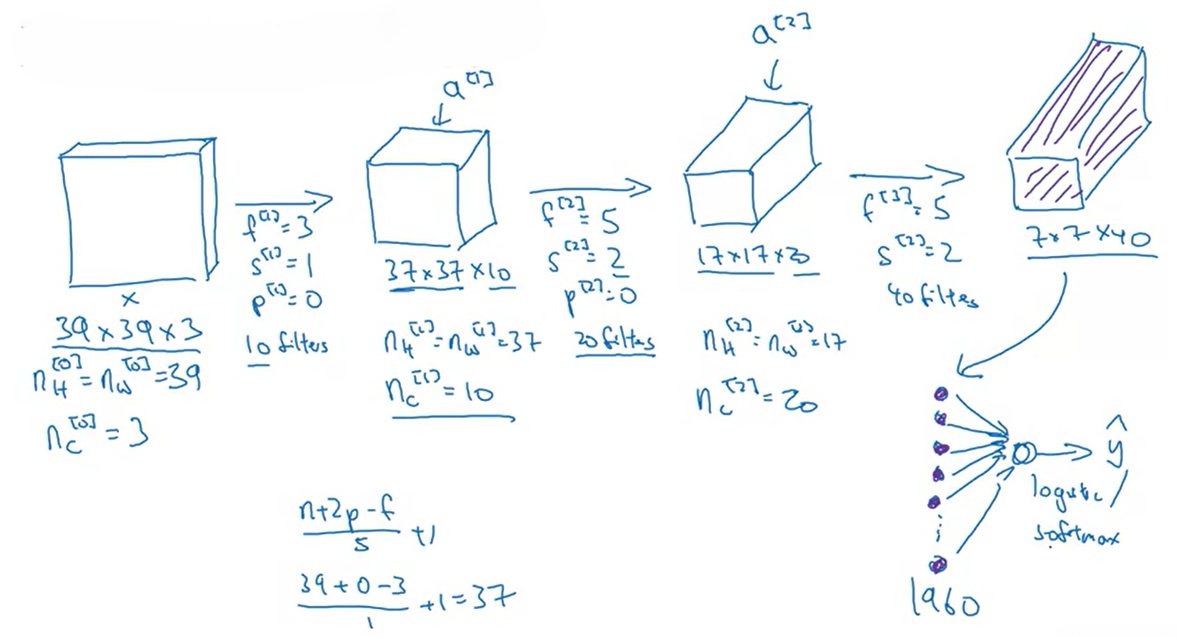
\includegraphics[width=\textwidth]{Images/ConvNet.png}
	\caption{Example of Simple Convolution Netwoks}
	\label{fig:28}
\end{figure}
\FloatBarrier

% ---------------- Pooling Layers ----------------------%
\subsection{Pooling Layers}
Other than convolutional layers, Convolutional Neural Networks (ConvNets) often use \textbf{pooling layers} to:
\begin{itemize}[nosep]
    \item Reduce the size of the representation.
    \item Speed up computation.
    \item Make feature detection more robust.
\end{itemize}

\subsubsection*{Max Pooling Example}
Suppose we have a $4 \times 4$ input and apply \textbf{max pooling} with a filter size $f=2$ and stride $s=2$. The output is a $2 \times 2$ representation:
\[
\text{Output}[i, j] = \max \text{(elements in the $2 \times 2$ region corresponding to filter location $i, j$)}.
\]

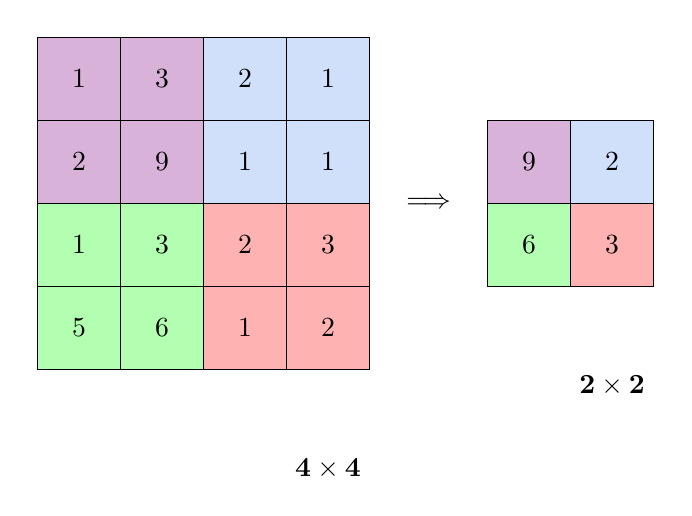
\begin{tikzpicture}[
    2d-arr/.style={matrix of nodes, row sep=-\pgflinewidth, column sep=-\pgflinewidth, nodes={draw}}
  ]

% Original image matrix
  \matrix (mtr) [2d-arr, nodes={draw, minimum width=3.0em, minimum height=3.0em, anchor=center}] {
|[fill=violet!30]| 1 &|[fill=violet!30]| 3 & |[fill=CornflowerBlue!30]| 2 & |[fill=CornflowerBlue!30]| 1 \\
|[fill=violet!30]| 2 &|[fill=violet!30]| 9 & |[fill=CornflowerBlue!30]| 1 & |[fill=CornflowerBlue!30]| 1  \\
|[fill=green!30]| 1 &|[fill=green!30]| 3 & |[fill=red!30]| 2 & |[fill=red!30]| 3  \\
|[fill=green!30]| 5 &|[fill=green!30]| 6 & |[fill=red!30]| 1 & |[fill=red!30]| 2  \\
};
\node[below=of mtr-4-4] {$\mathbf{4 \times 4}$};

% Arrow symbol
\node[right=0.6em of mtr] (arrow) {$\Longrightarrow$};

% Max Pooling Filter
\matrix (K) [2d-arr, right=0.6em of arrow, column sep=-\pgflinewidth, row sep=-\pgflinewidth, 
	nodes={draw, minimum width=3.0em, minimum height=3.0em, anchor=center}] {
|[fill=violet!30]| 9 & |[fill=CornflowerBlue!30]| 2  \\
|[fill=green!30]| 6 & |[fill=red!30]| 3  \\
};
\node[below=of K-2-2] {$\mathbf{2 \times 2}$};

\end{tikzpicture}

To compute each of the numbers on the right, we take the  max over a two by two regios i.e., we apply a filter size of 2 and stride by 2.

For instance:
\begin{itemize}[nosep]
    \item Top-left region: $\max(1, 3, 9, 4) = 9$.
    \item Top-right region: $\max(2, 1, 1, 1) = 2$.
    \item Bottom-left region: $\max(6, 5, 2, 1) = 6$.
    \item Bottom-right region: $\max(2, 3, 1, 2) = 3$.
\end{itemize}

\subsubsection*{Hyperparameters of Max Pooling}
The hyperparameters for max pooling are:
\begin{itemize}
    \item \textbf{Filter size} $f$: The dimension of the pooling region (e.g., $f = 2$ for $2 \times 2$ regions).
    \item \textbf{Stride} $s$: The step size for sliding the filter across the input.
    \item \textbf{Padding} $p$: Usually $p=0$ (no padding) in max pooling.
\end{itemize}

The output dimensions for an input of size $N_H \times N_W \times N_C$ are:
\[
N_H' = \frac{N_H - f}{s} + 1, \quad
N_W' = \frac{N_W - f}{s} + 1, \quad
N_C' = N_C.
\]

\subsubsection*{3D Inputs and Max Pooling}
For 3D inputs, max pooling is applied independently on each channel. For instance, if the input size is $5 \times 5 \times 2$, the output size will be $3 \times 3 \times 2$.

% Figure 29
\begin{figure}[h]
	\centering
	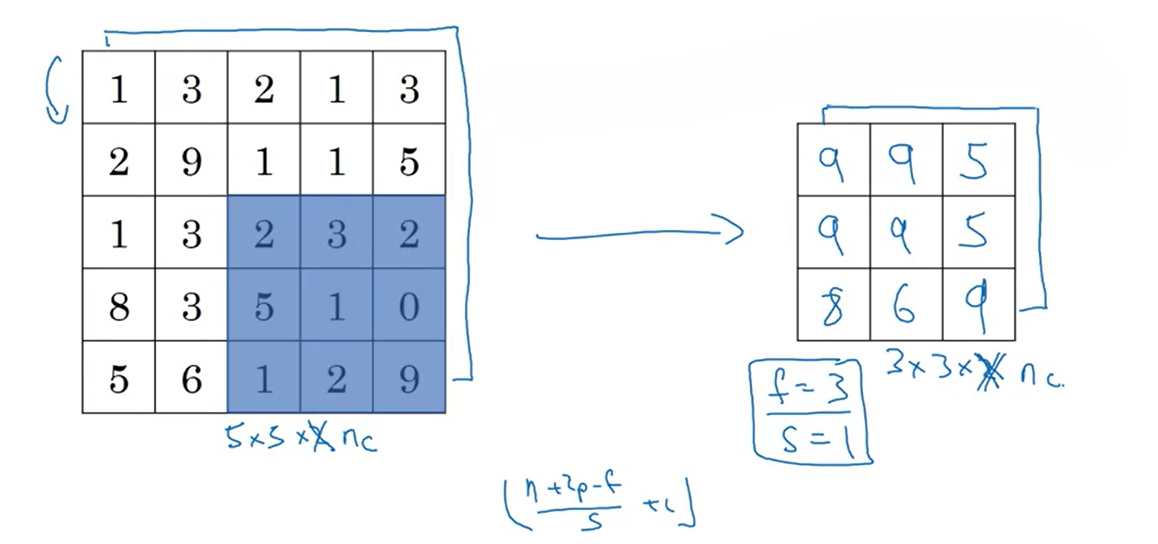
\includegraphics[width=\textwidth]{Images/3D Max Pooling.png}
	\caption{Max pooling for 3D Inputs}
	\label{fig:29}
\end{figure}
\FloatBarrier

\subsubsection*{Average Pooling}
Average pooling computes the average value within each filter region instead of the maximum. For example, with $f=2$ and $s=2$:
\[
\text{Output}[i, j] = \frac{\text{Sum of elements in the $2 \times 2$ region}}{4}.
\]

\subsubsection*{Key Properties of Pooling}
\begin{itemize}[nosep]
    \item No parameters are learned during pooling. It is a fixed operation defined by the hyperparameters $f$, $s$, and $p$.
    \item Max pooling is more commonly used than average pooling.
    \item Deep in a neural network, average pooling is occasionally used to collapse dimensions (e.g., $7 \times 7 \times 1000 \to 1 \times 1 \times 1000$).
\end{itemize}

\subsubsection*{Typical Hyperparameters}
\begin{itemize}[nosep]
    \item Common choices: $f=2$, $s=2$ (reduces height and width by a factor of $2$).
    \item Occasionally: $f=3$, $s=2$.
\end{itemize}

Pooling layers are essential components of ConvNets for reducing representation size and computational cost. They do not involve learning parameters and are defined entirely by their hyperparameters. 

% ---------------- CNN Example ----------------------%
\subsection{CNN Example}
Here, we discussed the building blocks of a convolutional neural network (CNN) inspired by LeNet-5 for handwritten digit recognition. The input is a $32 \times 32 \times 3$ RGB image, and the task is to classify digits (0 to 9) using a CNN architecture.

\subsubsection*{Architecture Details}
\begin{enumerate}[nosep]
    \item \textbf{Layer 1: Convolutional + Pooling Layer 1}
    \begin{itemize}
        \item Input: $32 \times 32 \times 3$ (RGB image).
        \item Convolutional Layer (Conv1):
        \begin{itemize}
            \item Filter size: $5 \times 5$.
            \item Stride: 1.
            \item Padding: None.
            \item Number of filters: 6.
            \item Output: $28 \times 28 \times 6$.
        \end{itemize}
        \item Max Pooling Layer (Pool1):
        \begin{itemize}
            \item Filter size: $2 \times 2$.
            \item Stride: 2.
            \item Output: $14 \times 14 \times 6$.
        \end{itemize}
        \item Combined Layer Output: $14 \times 14 \times 6$.
    \end{itemize}

    \item \textbf{Layer 2: Convolutional + Pooling Layer 2}
    \begin{itemize}
        \item Input: $14 \times 14 \times 6$.
        \item Convolutional Layer (Conv2):
        \begin{itemize}
            \item Filter size: $5 \times 5$.
            \item Stride: 1.
            \item Padding: None.
            \item Number of filters: 16.
            \item Output: $10 \times 10 \times 16$.
        \end{itemize}
        \item Max Pooling Layer (Pool2):
        \begin{itemize}
            \item Filter size: $2 \times 2$.
            \item Stride: 2.
            \item Output: $5 \times 5 \times 16$.
        \end{itemize}
        \item Combined Layer Output: $5 \times 5 \times 16$.
    \end{itemize}

    \item \textbf{Layer: Fully Connected Layer 1 (FC3)}
    \begin{itemize}
        \item Input: Flattened $5 \times 5 \times 16 = 400$ units.
        \item Output: $120$ units.
        \item Weights: $W_3$ of size $120 \times 400$.
        \item Bias: 120-dimensional vector.
    \end{itemize}

    \item \textbf{Layer: Fully Connected Layer 2 (FC4)}
    \begin{itemize}
        \item Input: $120$ units.
        \item Output: $84$ units.
    \end{itemize}

    \item \textbf{Output Layer}
    \begin{itemize}
        \item Input: $84$ units.
        \item Output: $10$ units (for classification of digits $0$ to $9$).
        \item Activation: Softmax.
    \end{itemize}
\end{enumerate}

% Figure 30
\begin{figure}[h]
	\centering
	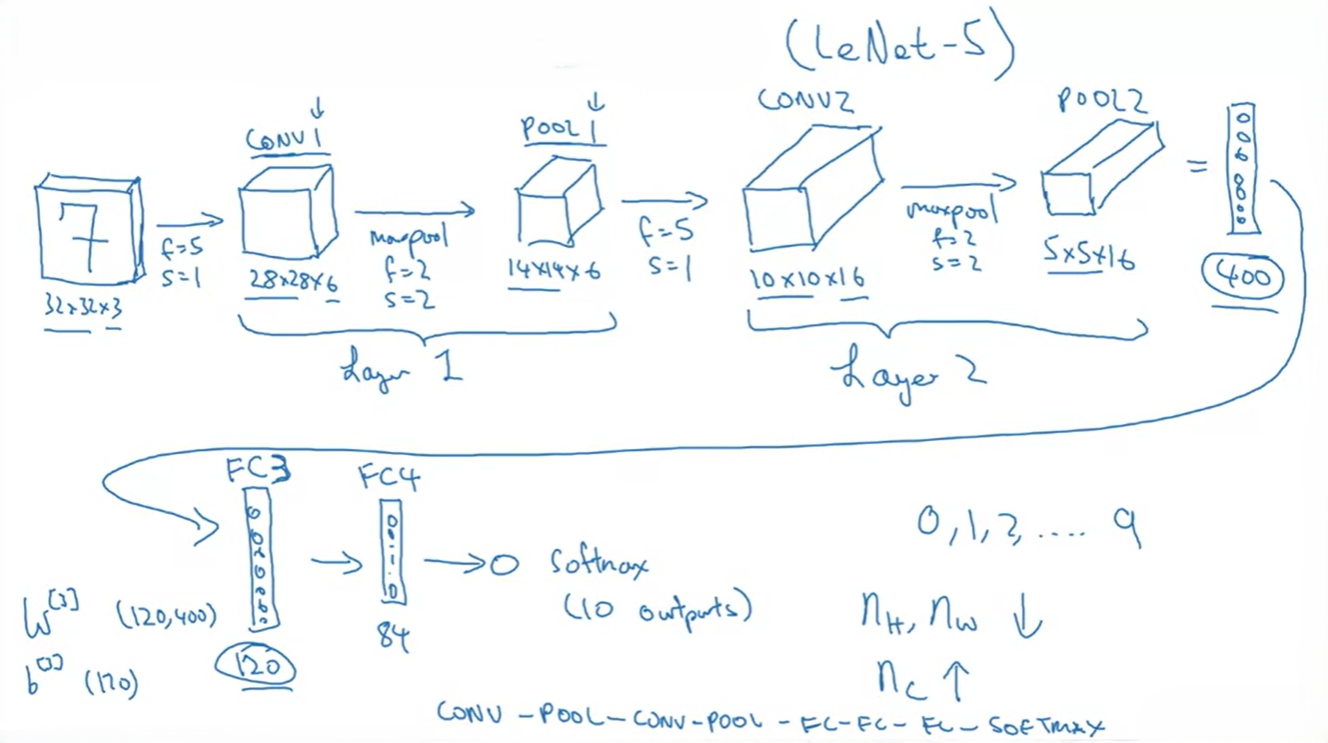
\includegraphics[width=0.95\textwidth]{Images/CNN Example.png}
	\caption{CNN Example Architecture}
	\label{fig:30}
\end{figure}

% Figure 31
\begin{figure}[h]
	\centering
	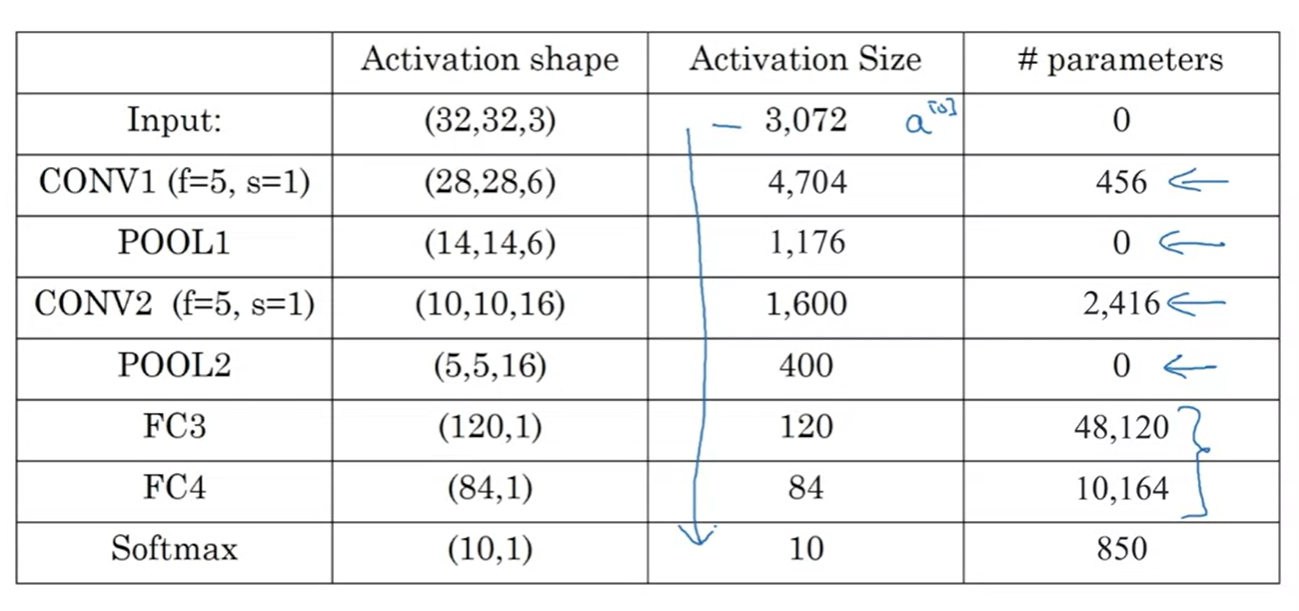
\includegraphics[width=0.85\textwidth]{Images/CNN Data.png}
	\caption{CNN Architecture Data}
	\label{fig:31}
\end{figure}

\FloatBarrier


\subsubsection*{Key Observations}
\begin{itemize}[nosep]
    \item \textbf{Pooling Layers:} No weights/parameters; only hyperparameters like filter size and stride.
    \item \textbf{Parameter Distribution:} Fully connected layers dominate in terms of the number of parameters compared to convolutional layers.
    \item \textbf{Activation Size:} Decreases progressively through the network, following a pattern:
    \[
    \text{Input: } 32 \times 32 \to 28 \times 28 \to 14 \times 14 \to 10 \times 10 \to 5 \times 5.
    \]
    \item \textbf{Number of Channels:} Increases as we go deeper in the network:
    \[
    3 \to 6 \to 16.
    \]
    \item \textbf{Common Architecture Pattern:}
    \begin{enumerate}
        \item Convolutional layers followed by pooling layers.
        \item Fully connected layers at the end.
        \item Final output: Softmax for classification.
    \end{enumerate}
\end{itemize}

\textbf{Question:} \\
\textbf{Q.1.} Suppose your input is a \( 256 \times 256 \) color (RGB) image, and you use a convolutional layer with 128 filters, each of size \( 7 \times 7 \). How many parameters does this hidden layer have (including the bias parameters)?

\textcolor{blue}{\textit{Solution:}}

The number of parameters in a convolutional layer can be calculated as:

\[
\text{Parameters} = (f \times f \times c + 1) \times k
\]

Where:
\begin{itemize}
    \item \( f \times f \) is the size of each filter (here, \( 7 \times 7 \)),
    \item \( c \) is the number of input channels (3 for RGB),
    \item \( k \) is the number of filters (128),
    \item The \( +1 \) accounts for the bias term in each filter.
\end{itemize}

Substituting the values:

\[
\text{Parameters} = (7 \times 7 \times 3 + 1) \times 128
\]
\[
\text{Parameters} = (147 + 1) \times 128 = 148 \times 128 = 18944
\]

Thus, the convolutional layer has \textbf{18,944} parameters, including the bias terms.

\textbf{Q.2.} Suppose your input is a \( 128 \times 128 \) grayscale image, and you are not using a convolutional network. If the first hidden layer has 256 neurons, each one fully connected to the input, how many parameters does this hidden layer have (including the bias parameters)?

\textcolor{blue}{\textit{Solution:}}

The number of parameters in a fully connected layer can be calculated as:

\[
\text{Parameters} = (\text{Number of input features} + 1) \times \text{Number of neurons}
\]

Where:
\begin{itemize}
    \item The number of input features is \( 128 \times 128 = 16384 \) (the total number of pixels in the grayscale image),
    \item The \( +1 \) accounts for the bias term for each neuron,
    \item The number of neurons in the hidden layer is 256.
\end{itemize}

Substituting the values:

\[
\text{Parameters} = (16384 + 1) \times 256 = 16385 \times 256 = 4194560
\]

Thus, the hidden layer has 4,194,560 parameters, including the bias terms.

\textbf{Q.3.} You have an input volume that is \( 121 \times 121 \times 16 \), and convolve it with 32 filters of size \( 4 \times 4 \), using a stride of 3 and no padding. What is the output volume?

\textcolor{blue}{\textit{Solution:}}

The output volume dimensions for a convolutional layer can be calculated using the formula:

\[
\text{Output size} = \left\lfloor \frac{\text{Input size} - \text{Filter size}}{\text{Stride}} \right\rfloor + 1
\]

Where:
\begin{itemize}
    \item \textbf{Input size} = \( 121 \) (for both height and width),
    \item \textbf{Filter size} = \( 4 \),
    \item \textbf{Stride} = \( 3 \),
    \item \textbf{No padding} means there is no additional padding around the input.
\end{itemize}

For the height and width:

\[
\text{Output height (or width)} = \left\lfloor \frac{121 - 4}{3} \right\rfloor + 1 = \left\lfloor \frac{117}{3} \right\rfloor + 1 = 39 + 1 = 40
\]

The depth of the output volume equals the number of filters, which is 32.

Thus, the output volume is:

\[
40 \times 40 \times 32
\]

\textbf{Q.4.} You have an input volume that is \( 31 \times 31 \times 32 \), and pad it using \texttt{pad=1}. What is the dimension of the resulting volume (after padding)?

\textcolor{blue}{\textit{Solution:}}

When padding is applied, the padding is added to each side of the height and width. The formula for calculating the dimensions after padding is:

\[
\text{Output size} = \text{Input size} + 2 \times \text{Padding}
\]

Where:
\begin{itemize}
    \item The \textbf{Input size} is \( 31 \) for both height and width,
    \item The \textbf{Padding} is \( 1 \).
\end{itemize}

For the height and width:

\[
\text{Output height (or width)} = 31 + 2 \times 1 = 33
\]

The depth remains unchanged as padding only affects the height and width, so the depth remains \( 32 \).

Thus, the resulting volume after padding is:

\[
33 \times 33 \times 32
\]

\textbf{Q.5.} You have a volume that is \( 121 \times 121 \times 32 \), and convolve it with 32 filters of size \( 5 \times 5 \), and a stride of 1. You want to use a ``same'' convolution. What is the padding?

\textcolor{blue}{\textit{Solution:}}

For a ``same'' convolution, the output size is the same as the input size. The formula for calculating the padding required for a ``same'' convolution is:

\[
\text{Padding} = \frac{\text{Filter size} - 1}{2}
\]

Where:
\begin{itemize}
    \item The \textbf{Filter size} is \( 5 \),
    \item The stride is \( 1 \).
\end{itemize}

Substituting the values:

\[
\text{Padding} = \frac{5 - 1}{2} = \frac{4}{2} = 2
\]

Thus, the padding required is 2.

% ---------------- Deep Convolutional Models ----------------------%
\section{Deep Convolutional Models: Case Studies}

% ---------------- Case Studies ----------------------%
\subsection{Case Studies}
% ---------------- Classic Networks ----------------------%
\subsection*{Classic Neural Network Architectures}
\subsubsection{LeNet-5}
LeNet-5 is one of the earliest convolutional neural network architectures designed to recognize handwritten digits. Below are its key features:
\begin{itemize}
    \item \textbf{Input:} $32 \times 32 \times 1$ (grayscale image).
    \item \textbf{Architecture:}
    \begin{itemize}
        \item Sequence: Conv $\Rightarrow$ Pool $\Rightarrow$ Conv $\Rightarrow$ Pool $\Rightarrow$ Fully Connected $\Rightarrow$ Fully Connected  $\Rightarrow$ Output
        \item \textbf{Convolutional Layer:} 6 filters of size $5 \times 5$, stride 1, no padding. Output: $28 \times 28 \times 6$.
        \item \textbf{Average Pooling:} Filter size $2 \times 2$, stride 2. Output: $14 \times 14 \times 6$.
        \item \textbf{Convolutional Layer:} 16 filters of size $5 \times 5$, stride 1, no padding. Output: $10 \times 10 \times 16$.
        \item \textbf{Average Pooling:} Filter size $2 \times 2$, stride 2. Output: $5 \times 5 \times 16$.
        \item Fully connected layers: 
	\begin{itemize}
	\item First fully connected layer connects each of these 400 nodes with every one of 120 neurons
	\item Second fully connected layer connects 120 nodes with every one of 84 neurons
	\item $400 \rightarrow 120 \rightarrow 84 \rightarrow 10$.
	\end{itemize}
    \end{itemize}
    \item \textbf{Output:} 10-way classification for digits (0–9) using a softmax function.
    \item \textbf{Parameters:} Approximately 60,000.
    \item \textbf{Key Patterns:} Reduction in spatial dimensions (height \& width) and increase in channels as layers deepen.
    \item \textbf{Historical Notes:}
    \begin{itemize}
        \item Used \textbf{sigmoid} and \textbf{tanh} nonlinearities (ReLU is used in modern networks).
        \item Complex filter-channel connections due to computational limitations.
        \item Included a nonlinearity after pooling.
    \end{itemize}
\end{itemize}

% Figure 32
\begin{figure}[h]
	\centering
	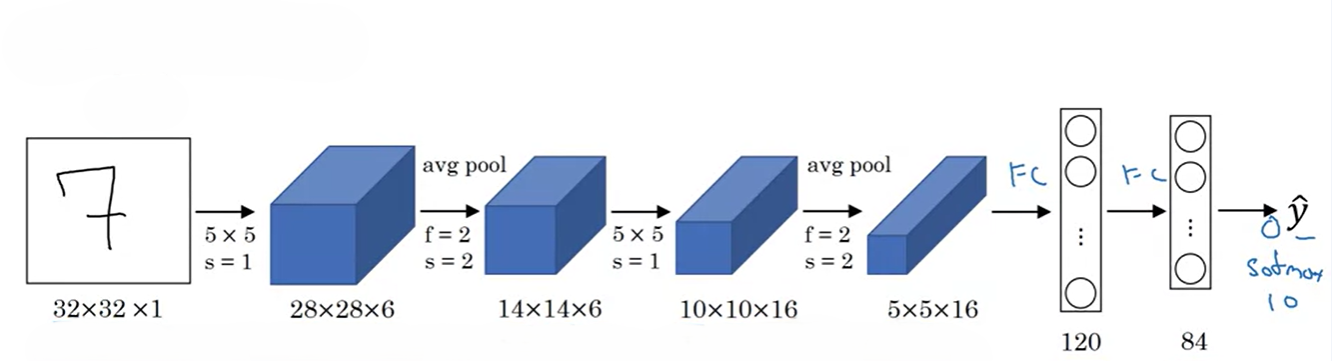
\includegraphics[width=\textwidth]{Images/LeNet-5.png}
	\caption{LeNet - 5 Architecture}
	\label{fig:32}
\end{figure}

\FloatBarrier

\subsubsection{AlexNet}
AlexNet brought significant advancements in deep learning for computer vision. It was trained on the ImageNet dataset and introduced key improvements.
\begin{itemize}
    \item \textbf{Input:} $227 \times 227 \times 3$ (RGB image).
    \item \textbf{Architecture:}
    \begin{itemize}
        \item Convolutional Layer: 96 filters of size $11 \times 11$, stride 4. Output: $55 \times 55 \times 96$.
        \item Max Pooling: Filter size $3 \times 3$, stride 2. Output: $27 \times 27 \times 96$.
        \item Convolutional Layer: $5 \times 5$ filters, same padding. Output: $27 \times 27 \times 256$.
        \item Max Pooling: Output: $13 \times 13 \times 256$.
        \item Several additional convolutional layers, max-pooling, and fully connected layers follow.
    \end{itemize}
    \item \textbf{Output:} 1000-way softmax classification for ImageNet classes.
    \item \textbf{Parameters:} Approximately 60 million.
    \item \textbf{Key Improvements:}
    \begin{itemize}
        \item Use of \textbf{ReLU} activation instead of sigmoid/tanh.
        \item Trained on two GPUs with layer-wise distribution of computations.
        \item Introduced \textbf{Local Response Normalization} (not commonly used today).
    \end{itemize}
    \item \textbf{Impact:} Demonstrated the power of deep learning for computer vision.
\end{itemize}

% Figure 33
\begin{figure}[h]
	\centering
	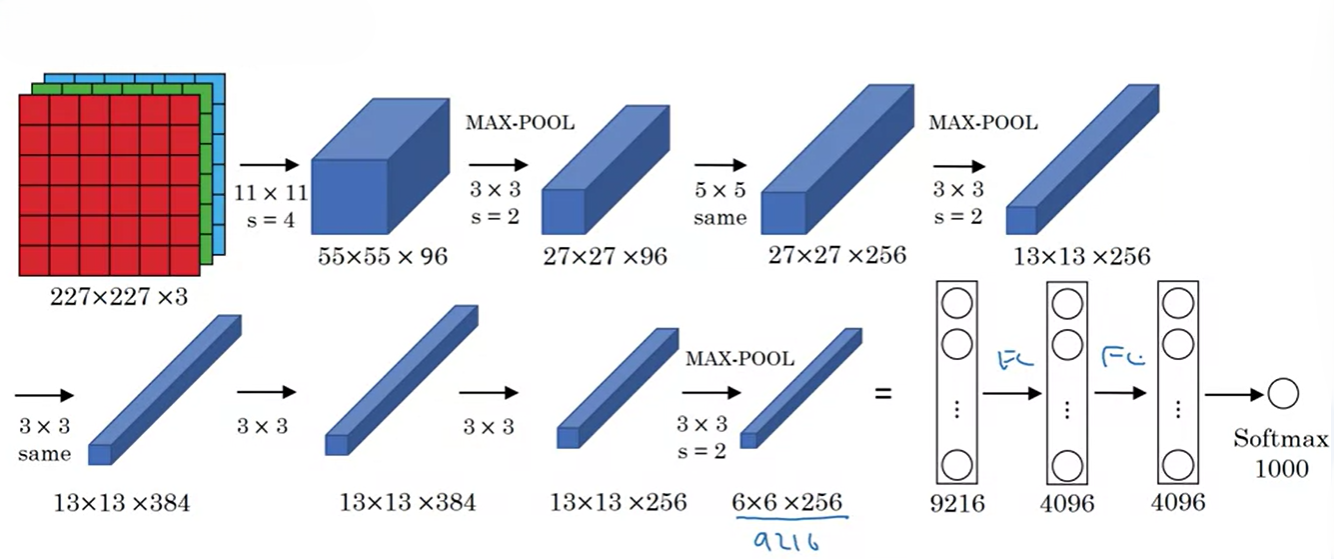
\includegraphics[width=\textwidth]{Images/AlexNet.png}
	\caption{AlexNet Architecture}
	\label{fig:33}
\end{figure}

\subsubsection{VGG-16}
VGG-16 emphasized simplicity and uniformity in architecture design.
\begin{itemize}
    \item \textbf{Input:} $224 \times 224 \times 3$ (RGB image).
    \item \textbf{Architecture:}
    \begin{itemize}[nosep]
        \item All convolutional layers use $3 \times 3$ filters, stride 1, and same padding.
        \item Max-pooling layers use $2 \times 2$ filters, stride 2.
        \item Convolutional layers increase the number of filters:
        \begin{itemize}
            \item First two layers: 64 filters.
            \item Next two layers: 128 filters.
            \item Next three layers: 256 filters.
            \item Next three layers: 512 filters.
        \end{itemize}
        \item Fully connected layers: 4096 units followed by a softmax layer.
    \end{itemize}
    \item \textbf{Output:} 1000-way classification for ImageNet classes.
    \item \textbf{Parameters:} Approximately 138 million.
    \item \textbf{Key Features:}
    \begin{itemize}
        \item Simplicity: Fixed filter sizes and strides.
        \item Doubling of filters in successive stages (up to 512).
        \item Uniform architecture design.
    \end{itemize}
    \item \textbf{Variants:} VGG-19 (deeper but similar performance).
\end{itemize}

% Figure 34
\begin{figure}[h]
	\centering
	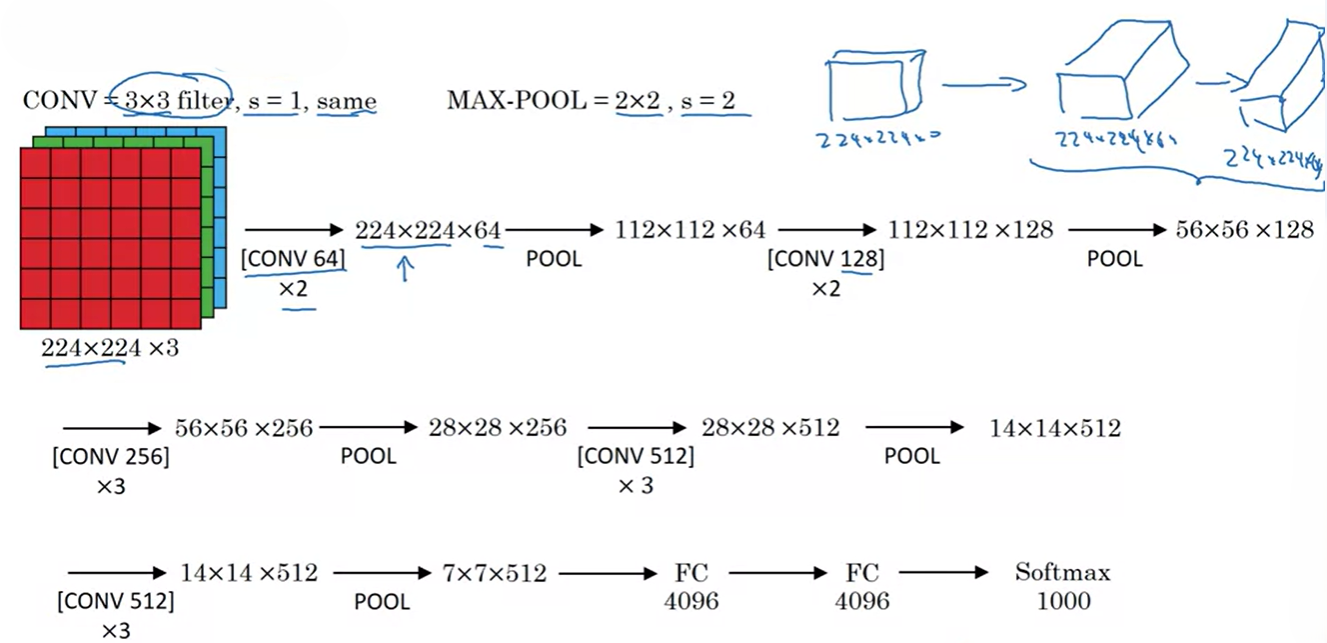
\includegraphics[width=\textwidth]{Images/VGG-16.png}
	\caption{VGG-16 Architecture}
	\label{fig:34}
\end{figure}

\subsubsection{Comparison of Architectures}
\begin{itemize}[nosep]
    \item \textbf{LeNet-5:} Small network with $\sim$60,000 parameters, designed for grayscale digit recognition.
    \item \textbf{AlexNet:} Introduced ReLU, GPU training, and scaled up to 60M parameters.
    \item \textbf{VGG-16:} Uniform design with 138M parameters, using $3 \times 3$ filters throughout.
\end{itemize}

% ---------------- ResNets ----------------------%
\subsection*{ResNets}
Very deep neural networks are challenging to train due to \textbf{vanishing} and \textbf{exploding gradient} problems. To address this, \textbf{skip connections} (or \textbf{shortcuts}) were introduced. Skip connections allow activations from one layer to directly feed into another, bypassing intermediate layers. This concept is central to the architecture of \textbf{ResNets (Residual Networks)}, enabling training of networks with over 100 layers.

\subsubsection{Residual Blocks}
A \textbf{residual block} forms the building block of ResNets. Here's how it works:
\begin{itemize}[nosep]
    \item Start with activations from layer $a^{[l]}$.
    \item Compute $z^{[l+1]}$ using the linear operation:
    \[
    z^{[l+1]} = W^{[l+1]}a^{[l]} + b^{[l+1]}.
    \]
    \item Apply a ReLU non-linearity:
    \[
    a^{[l+1]} = g(z^{[l+1]}),
    \]
    where $g$ is the ReLU function.
    \item Repeat for the next layer to compute $z^{[l+2]}$ and $a^{[l+2]}$.
\end{itemize}
In a \textbf{plain network}, information must pass through these layers sequentially. However, in a \textbf{residual network}, a shortcut connection adds $a^{[l]}$ directly to $z^{[l+2]}$:
\[
a^{[l+2]} = g(z^{[l+2]} + a^{[l]}).
\]
This shortcut bypasses the main path, allowing information to flow more effectively.

% Figure 35
\begin{figure}[h]
	\centering
	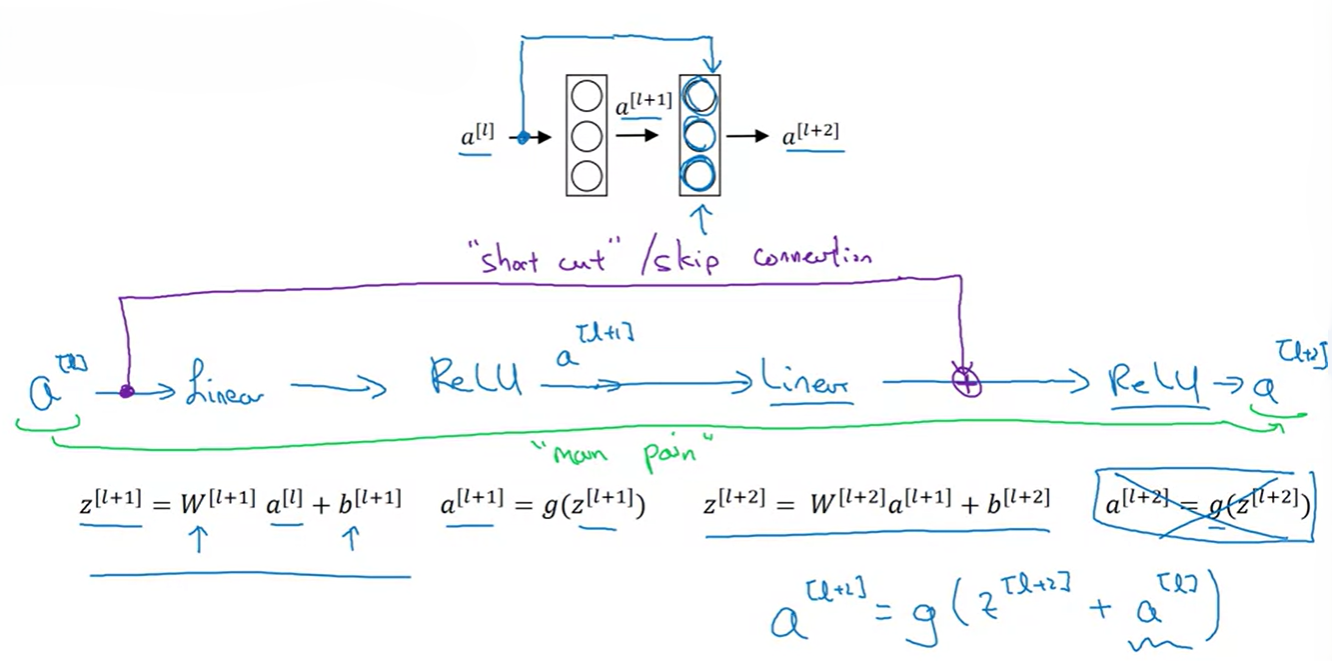
\includegraphics[width=\textwidth]{Images/Residual Block.png}
	\caption{Residual Block}
	\label{fig:35}
\end{figure}

\begin{figure}[h]
\centering
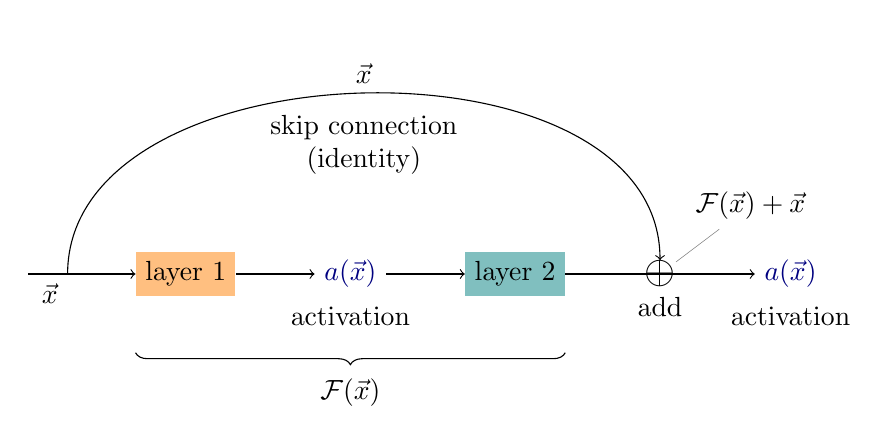
\begin{tikzpicture}

  \node[fill=orange!50] (l1) {layer 1};
  \node[blue!50!black, right=of l1, label={below:activation}] (act1) {$a(\vec x)$};
  \node[fill=teal!50, right=of act1] (l2) {layer 2};
  \node[right=of l2, font=\Large, label={below:add}, inner sep=0, pin={60:$\mathcal F(\vec x) + \vec x$}] (add) {$\oplus$};
  \node[blue!50!black, right=of add, label={below:activation}] (act2) {$a(\vec x)$};

  \draw[->] (l1) -- (act1);
  \draw[->] (act1) -- (l2);
  \draw[<-] (l1) -- ++(-2,0) node[below, pos=0.8] {$\vec x$};
  \draw[->] (l2) -- (act2) node[above, pos=0.8] {};
  \draw[->] ($(l1)-(1.5,0)$) to[out=90, in=90] node[below=1ex, midway, align=center] {skip connection\\(identity)} node[above, midway] {$\vec x$} (add);
  \draw[decorate, decoration={brace, amplitude=1ex, raise=1cm}] (l2.east) -- node[midway, below=1.2cm] {$\mathcal F(\vec x)$} (l1.west);
\end{tikzpicture}
  \caption{Illustration of skip connection in a residual block}
  \label{fig:36}
\end{figure}
\FloatBarrier

\subsubsection{Key Features of Residual Networks}
\begin{itemize}
    \item \textbf{Skip Connections:} Enable direct flow of information from earlier to deeper layers, addressing the vanishing/exploding gradient problem.
    \item \textbf{Residual Learning:} Instead of learning the full transformation, residual blocks learn a residual function, simplifying optimization.
    \item \textbf{Stacking Residual Blocks:} ResNets are built by stacking multiple residual blocks. For example, a ResNet with 5 residual blocks might look like shown in \textbf{Fig. \ref{fig:37}}:
    \begin{itemize}
        \item Each block adds a skip connection to a pair of layers.
    \end{itemize}

	% Figure 37
	\begin{figure}[h]
		\centering
		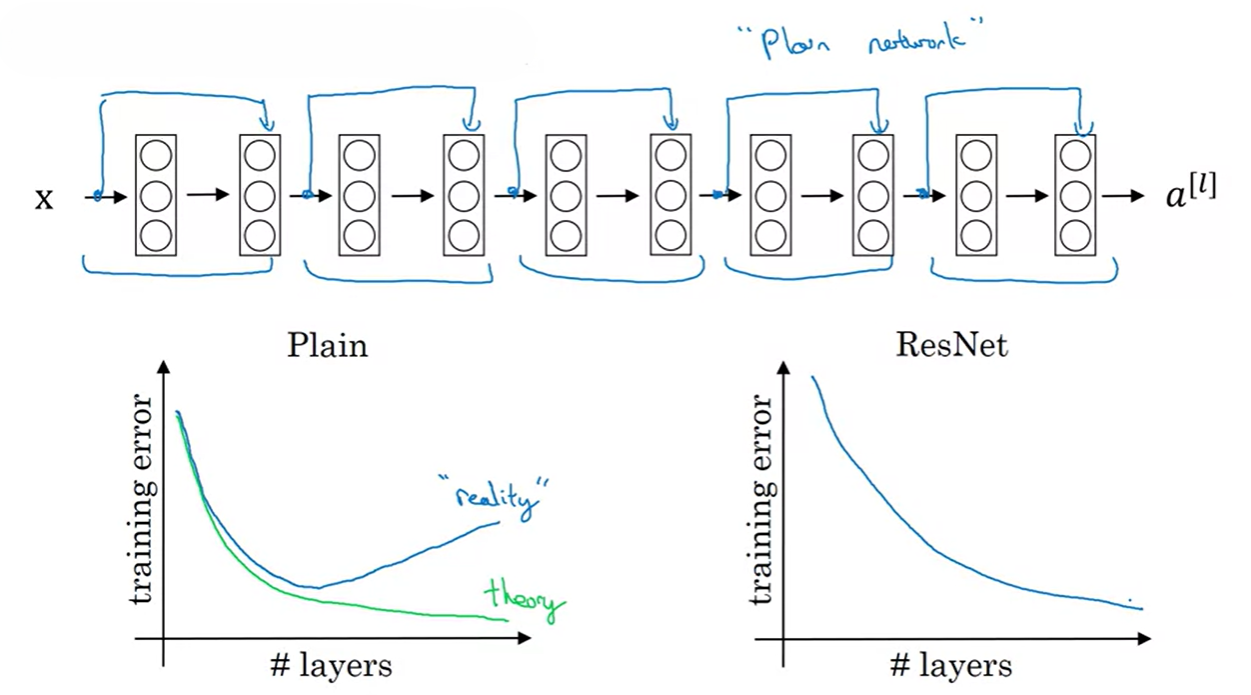
\includegraphics[width=\textwidth]{Images/Residual Networks.png}
		\caption{Residual Networks}
		\label{fig:37}
	\end{figure}
	\FloatBarrier

    \item \textbf{Training Behavior:} 
    \begin{itemize}
        \item In plain networks, training error increases as the number of layers grows due to optimization challenges.
        \item ResNets enable the training error to decrease even with very deep networks.
    \end{itemize}
\end{itemize}

\subsubsection{Practical Impact of ResNets}
\begin{itemize}
    \item ResNets have been successfully trained with over 100 layers, and experimental setups include networks with over 1000 layers.
    \item By addressing gradient problems, ResNets ensure better performance without significant loss in training efficiency.
    \item While deeper networks may plateau in performance gains, ResNets remain highly effective for training deep architectures.
\end{itemize}

ResNets revolutionized deep learning by enabling the training of very deep neural networks through skip connections and residual learning. These ideas have addressed critical challenges in optimization, such as vanishing gradients, and have paved the way for efficient training of deep architectures. Experimenting with ResNets will further solidify your understanding of these concepts.

% ---------------- Inception Network ----------------------%
\subsection*{Inception Network}
When designing a convolutional layer, you might face the challenge of choosing the filter size: one-by-one, three-by-three, five-by-five, or even deciding whether to use a pooling layer. The inception network proposes to solve this dilemma by doing all of them. This approach makes the architecture more complex but is highly effective.

\subsubsection*{Overview of the Inception Module}
Given an input volume of size $28 \times 28 \times 192$, the inception module applies:

\begin{itemize}[nosep]
    \item A $1 \times 1$ convolution producing $28 \times 28 \times 64$.
    \item A $3 \times 3$ convolution producing $28 \times 28 \times 128$.
    \item A $5 \times 5$ convolution producing $28 \times 28 \times 32$.
    \item A pooling layer producing $28 \times 28 \times 32$.
\end{itemize}

To maintain consistent spatial dimensions ($28 \times 28$), padding and strides are carefully chosen:
\begin{itemize}[nosep]
    \item Padding is used for both convolutions and pooling.
    \item Stride is set to 1 for pooling.
\end{itemize}

The outputs are concatenated along the channel dimension, resulting in a volume of size $28 \times 28 \times 256$.

\subsubsection*{Computational Cost of the Inception Module}
One limitation of the inception module is its computational cost. Let us consider the $5 \times 5$ convolution:

\subsubsection*{Original Design}
For an input volume of $28 \times 28 \times 192$, a $5 \times 5$ convolution with 32 filters produces an output of $28 \times 28 \times 32$. The computational cost is:
\begin{align*}
\text{Computational cost} &= \text{ \#filter params * \# filter positions * \# of filters}  \\
 & = 28 \times 28 \times 32 \times (5 \times 5 \times 192) = 120 \text{ million multiplications}.
\end{align*}

\subsubsection*{Using Bottleneck Layers}
To reduce computational cost, the inception module incorporates $1 \times 1$ convolutions, known as \textbf{bottleneck layers}. This technique reduces the number of channels before applying the $5 \times 5$ convolution:
\begin{enumerate}
    \item Apply a $1 \times 1$ convolution to shrink the input volume to $28 \times 28 \times 16$:
    \[
    28 \times 28 \times 16 \times (1 \times 1 \times 192) = 2.4 \text{ million multiplications}.
    \]
    \item Apply the $5 \times 5$ convolution to the reduced volume:
    \[
    28 \times 28 \times 32 \times (5 \times 5 \times 16) = 10 \text{ million multiplications}.
    \]
\end{enumerate}

The total cost is:
\[
2.4 + 10 = 12.4 \text{ million multiplications}.
\]

This is approximately one-tenth the cost of the original design.

\subsubsection*{Effectiveness of Bottleneck Layers}
Shrinking the representation size dramatically might seem harmful, but experiments show that as long as the bottleneck layer is implemented within reasonable limits, the performance of the neural network remains unaffected while computation costs are significantly reduced.

The inception module allows the network to combine multiple filter sizes ($1 \times 1$, $3 \times 3$, $5 \times 5$) and pooling, avoiding the need to choose a specific filter size. By using bottleneck layers, the computational cost is significantly reduced without sacrificing performance. These ideas form the core of the inception network.

% Figure 38
\begin{figure}[h]
	\centering
	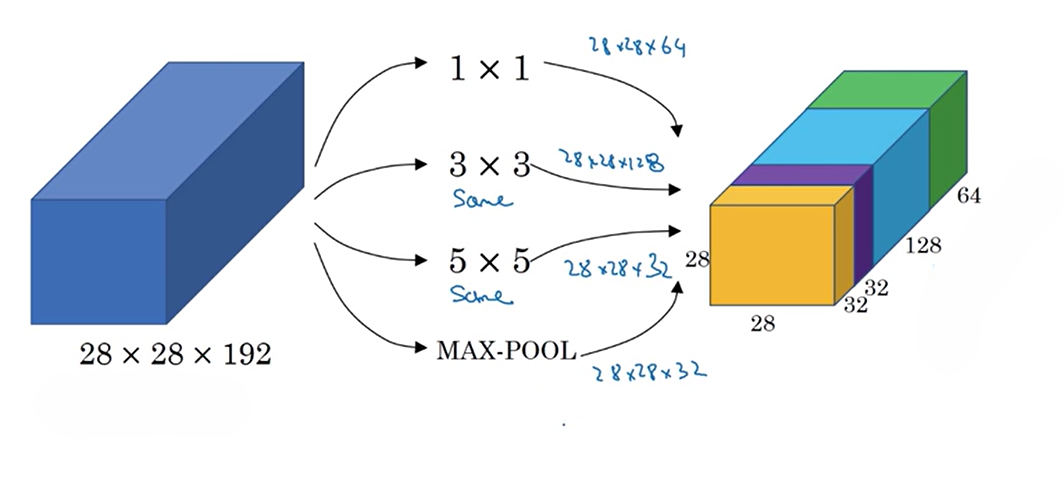
\includegraphics[width=0.85\textwidth]{Images/Inception Network.png}
	\caption{Inception Network}
	\label{fig:38}
\end{figure}
\FloatBarrier

% ---------------- MobileNet ----------------------%
\subsection*{MobileNets and Depthwise Separable Convolution}
\textbf{MobileNets} is a foundational convolutional neural network architecture used in computer vision. MobileNets are specifically designed for low-compute environments, such as mobile phones, enabling efficient deployment of neural networks. 

\subsubsection*{Why MobileNets?}
Many neural networks, such as ResNet and InceptionNet, are computationally expensive. If your deployment device has limited computational resources (e.g., less powerful CPU or GPU), MobileNet's architecture, with \textbf{depthwise separable convolutions}, can provide significant computational savings while maintaining performance.

\subsubsection*{Normal Convolution}
Consider an input image of size $n \times n \times n_c$, where $n_c$ is the number of channels (e.g., $6 \times 6 \times 3$). A filter of size $f \times f \times n_c$ (e.g., $3 \times 3 \times 3$) is convolved across the image. The steps include:
\begin{itemize}[nosep]
    \item Place the filter at each position on the image.
    \item Perform $f \times f \times n_c$ multiplications (e.g., $3 \times 3 \times 3 = 27$).
    \item Sum the results to produce one output value.
    \item Repeat for all positions to compute the output of size $n_{\text{out}} \times n_{\text{out}} \times n_c'$, where $n_{\text{out}}$ is smaller due to no padding (e.g., $4 \times 4 \times 5$).
\end{itemize}

\subsubsection*{Computational Cost}
The total cost is:
\[
f \times f \times n_c \times n_{\text{out}} \times n_{\text{out}} \times n_c'
\]
For example, with $f = 3$, $n_c = 3$, $n_{\text{out}} = 4$, and $n_c' = 5$, the cost is:
\[
3 \times 3 \times 3 \times 4 \times 4 \times 5 = 2160 \text{ multiplications.}
\]

% Figure 39
\begin{figure}[h]
	\centering
	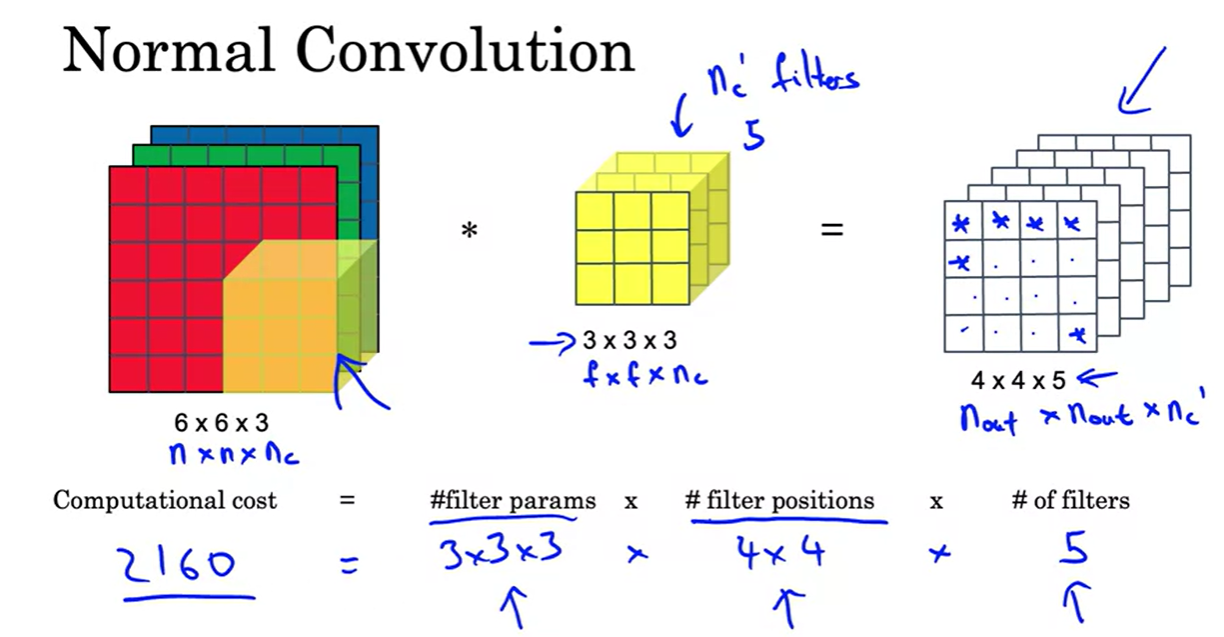
\includegraphics[width=0.85\textwidth]{Images/Normal Convolution.png}
	\caption{Normal Convolution}
	\label{fig:39}
\end{figure}
\FloatBarrier

\subsubsection*{Depthwise Separable Convolution}
In contrast to the normal convolution, the depthwise separable convolution has two steps. The first step is to use a depthwise convolution, followed by a pointwise convolution. It is these two steps which together make up this depthwise separable convolution. 

Depthwise separable convolution splits the normal convolution into two steps:
\begin{enumerate}[nosep]
    \item \textbf{Depthwise Convolution}
    \item \textbf{Pointwise Convolution}
\end{enumerate}

\subsubsection*{Step 1: Depthwise Convolution}
\begin{itemize}[nosep]
    \item Instead of $f \times f \times n_c$ filters, use $f \times f$ filters (one per channel).
    \item Apply each filter to its corresponding channel.
    \item Output size: $n_{\text{out}} \times n_{\text{out}} \times n_c$.
\end{itemize}

\subsubsection*{Computational Cost}
\[
f \times f \times n_{\text{out}} \times n_{\text{out}} \times n_c
\]
For $f = 3$, $n_{\text{out}} = 4$, and $n_c = 3$, the cost is:
\[
3 \times 3 \times 4 \times 4 \times 3 = 432 \text{ multiplications.}
\]

% Figure 40
\begin{figure}[h]
	\centering
	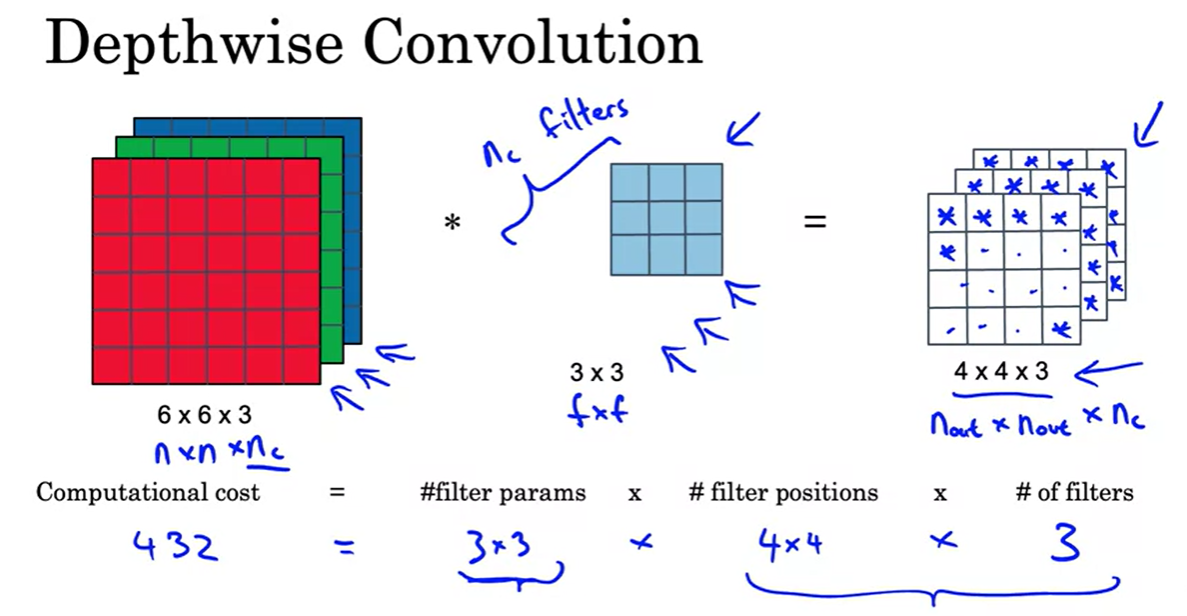
\includegraphics[width=0.85\textwidth]{Images/Depthwise Convolution.png}
	\caption{Depthwise Convolution}
	\label{fig:40}
\end{figure}
\FloatBarrier

\subsubsection*{Step 2: Pointwise Convolution}
In the Pointwise Convolution, we take the intermediate set of values.i.e., output of Depthwise Convolution ($n_{\text{out}} \times n_{\text{out}} \times n_c'$) and convolve it with a filter that is $1 \times 1 \times n_c$, 1 by 1 by 3 in this case.
\begin{itemize}[nosep]
    \item Use $1 \times 1 \times n_c$ filters.
    \item Convolve each filter across all positions to produce $n_c'$ output channels.
    \item Output size: $n_{\text{out}} \times n_{\text{out}} \times n_c'$.
\end{itemize}

\subsubsection*{Computational Cost}
\[
1 \times 1 \times n_c \times n_{\text{out}} \times n_{\text{out}} \times n_c'
\]
For $n_c = 3$, $n_{\text{out}} = 4$, and $n_c' = 5$, the cost is:
\[
1 \times 1 \times 3 \times 4 \times 4 \times 5 = 240 \text{ multiplications.}
\]

% Figure 41
\begin{figure}[h]
	\centering
	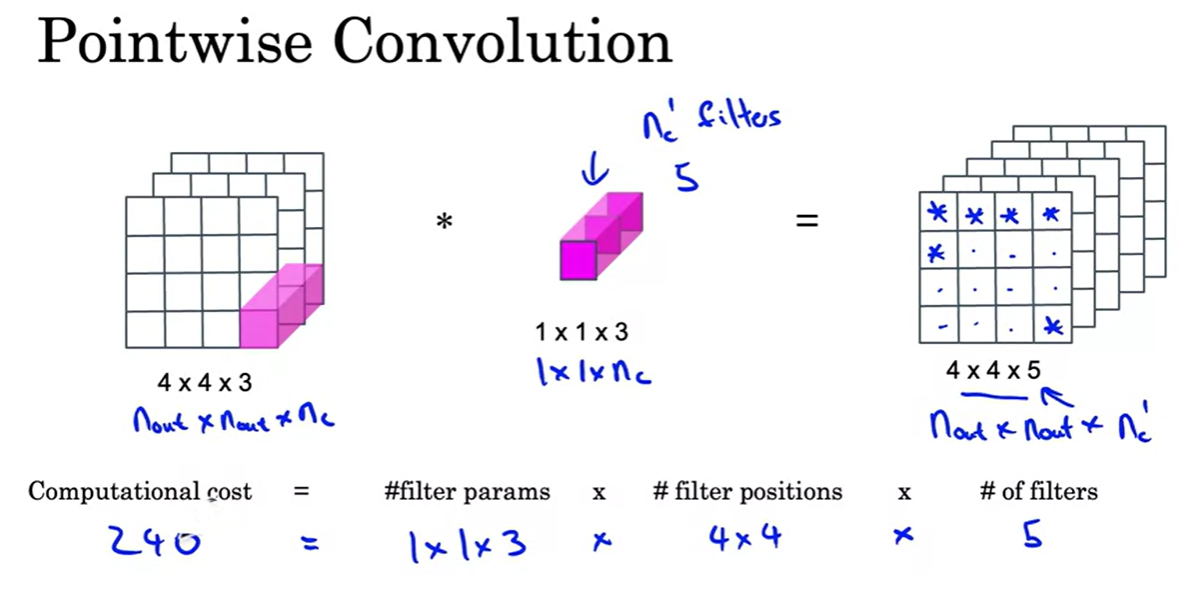
\includegraphics[width=0.85\textwidth]{Images/Pointwise Convolution.png}
	\caption{Pointwise Convolution}
	\label{fig:41}
\end{figure}
\FloatBarrier

\subsubsection*{Total Computational Cost}
\[
\text{Depthwise: } 432, \quad \text{Pointwise: } 240, \quad \text{Total: } 432 + 240 = 672 \text{ multiplications.}
\]
This is significantly less than the normal convolution cost of 2160 multiplications:
\[
\frac{672}{2160} \approx 0.31 \, (31\% \text{ of the original cost}).
\]

\subsubsection*{General Formula}
The computational cost ratio between depthwise separable and normal convolution is:
\[
\frac{1}{n_c'} + \frac{1}{f^2}
\]

Depthwise separable convolution reduces computational cost while maintaining the same input-output dimensions as normal convolution. It is a core building block of MobileNets, enabling efficient inference on low-compute devices.


% ---------------- EfficientNet ----------------------%
\subsection*{EfficientNet}
MobileNet V1 and V2 introduced a way to implement neural networks that are more computationally efficient. However, in practical applications, the challenge arises in tuning these architectures to fit specific devices. For instance, one might implement a computer vision algorithm for:
\begin{itemize}[nosep]
    \item Different brands of mobile phones with varying compute resources.
    \item Different edge devices with distinct computational constraints.
\end{itemize}

Depending on the available computational budget, you may need a larger network for higher accuracy or a smaller network for faster execution at the cost of some accuracy. The question is: \textit{How can neural networks be automatically scaled up or down for a particular device?}

\subsubsection*{EfficientNet: A Solution for Scalable Neural Networks}
EfficientNet provides a method to systematically scale a baseline neural network architecture to meet specific computational requirements. Let’s assume the baseline architecture includes:
\begin{itemize}[nosep]
    \item \textbf{Input resolution} denoted as \(r\),
    \item \textbf{Network depth} denoted as \(d\),
    \item \textbf{Layer width} denoted as \(w\).
\end{itemize}

The authors of EfficientNet, Mingxing Tan and Quoc Le, identified three primary ways to scale a neural network:
\begin{enumerate}[nosep]
    \item Use higher resolution input images (\(r\)).
    \item Increase the depth of the neural network (\(d\)).
    \item Increase the width of the layers (\(w\)).
\end{enumerate}

The challenge is determining the best combination of \(r\), \(d\), and \(w\) for a given computational budget. EfficientNet introduces \textbf{compound scaling}, which allows simultaneous scaling of resolution, depth, and width. The key question is: \textit{At what rates should \(r\), \(d\), and \(w\) be scaled?}

\subsubsection*{Compound Scaling Trade-Offs}
When scaling up or down \(r\), \(d\), and \(w\), there are multiple trade-offs to consider:
\begin{itemize}[nosep]
    \item Should the resolution (\(r\)) be doubled while keeping depth (\(d\)) and width (\(w\)) constant?
    \item Should the depth (\(d\)) be doubled while keeping resolution and width constant?
    \item Should all three parameters (\(r\), \(d\), \(w\)) be scaled simultaneously, and if so, by what proportions?
\end{itemize}

EfficientNet helps determine the optimal trade-offs between these parameters to achieve the best performance within the computational budget. EfficientNet can adapt neural networks to specific devices by leveraging open-source implementations. These implementations enable practitioners to:
\begin{itemize}[nosep]
    \item Choose suitable trade-offs between \(r\), \(d\), and \(w\).
    \item Build scalable neural networks for mobile devices, embedded systems, and other resource-constrained environments.
\end{itemize}

With MobileNet, one can design computationally efficient layers, and with EfficientNet, these architectures can be scaled to fit device-specific requirements. These tools empower developers to build neural networks for a wide range of applications, including mobile and embedded devices where computational and memory resources are limited.

% ---------------- Practical Advice for Using ConvNets ----------------------%
\subsection{Practical Advice for Using ConvNets}
% ---------------- Using Open-Source Implementation ----------------------%
\subsection*{Using Open-Source Implementation}
If you encounter a research paper with results you want to build upon, it is highly recommended to look online for an open-source implementation. This approach can save significant time compared to reimplementing the architecture from scratch. While reimplementation can be a valuable learning exercise, starting with open-source code can help you get started on a project much faster.

\subsubsection*{Advantages of Using Open-Source Code}
\begin{itemize}
    \item \textbf{Pretrained Models:} Many open-source implementations include pretrained models, which can save you the time and computational resources required to train from scratch. These models are often trained on large datasets using multiple GPUs.
    \item \textbf{Transfer Learning:} Pretrained models can be used for transfer learning, allowing you to adapt a pretrained network to your specific application. Transfer learning will be discussed in more detail in the next section.
    \item \textbf{Time Efficiency:} Starting with open-source code significantly accelerates the development process for new projects.
\end{itemize}

\subsubsection*{Common Workflow for Computer Vision Applications}
When developing a computer vision application, the following steps are common:
\begin{enumerate}
    \item Select an architecture that fits your needs. This could be one learned in a course, from literature, or recommended by a colleague.
    \item Search for an open-source implementation of the architecture and download it from GitHub.
    \item Utilize the pretrained weights, if available, to perform transfer learning or fine-tuning for your specific task.
\end{enumerate}

% ---------------- Transfer Learning ----------------------%
\subsection*{Transfer Learning}
When building computer vision applications, training a neural network from scratch using random initialization is often inefficient. Instead, you can make much faster progress by using pre-trained weights from networks trained on large datasets. This approach is known as \textbf{transfer learning}. 

The computer vision research community has made numerous datasets such as ImageNet, MS COCO, and Pascal VOC publicly available. These datasets have been used to train various models, often taking weeks or months on high-performance GPUs. By leveraging these pre-trained weights, you can initialize your own models effectively, saving significant computational time and effort.

To apply transfer learning, follow these steps:

\subsubsection*{Example: Building a Cat Detector}
Consider building a classifier to identify three classes: \textit{Tigger}, \textit{Misty}, or \textit{Neither}. If you have a small training set, transfer learning becomes invaluable:
\begin{itemize}[nosep]
    \item Download a pre-trained network and its weights (e.g., a model trained on ImageNet).
    \item Replace the original softmax layer with a new one that outputs the desired three classes.
    \item Freeze all layers except the softmax layer. This means the parameters in the frozen layers will not be updated during training.
    \item Train only the softmax layer using your small dataset.
\end{itemize}

Most deep learning frameworks support freezing layers through parameters like \texttt{trainable=false} or \texttt{freeze=true}. This allows you to specify which layers remain unchanged during training.

\subsubsection*{Pre-computation of Activations}
Because the earlier layers are frozen, they act as a fixed function mapping input images to feature representations. To speed up training:
\begin{itemize}[nosep]
    \item Pre-compute activations from the frozen layers for all training images.
    \item Save these activations to disk.
    \item Train the softmax layer using these pre-computed features, avoiding the need to recompute them during each training epoch.
\end{itemize}

\subsubsection*{Larger Training Sets}
If you have a larger labeled dataset:
\begin{itemize}[nosep]
    \item Freeze fewer layers and train more layers closer to the output. 
    \item Replace the final layers with new ones tailored to your problem.
    \item Use the pre-trained weights of the unfrozen layers as initialization and fine-tune them with gradient descent.
\end{itemize}

\subsubsection*{Extremely Large Training Sets}
If you have a very large labeled dataset and a significant computational budget:
\begin{itemize}[nosep]
    \item Use the pre-trained weights as initialization for the entire network.
    \item Train the entire network (including all layers) using your dataset.
    \item Replace the original softmax layer with one that matches your output classes.
\end{itemize}

\subsubsection*{Advantages of Transfer Learning}
\begin{itemize}[nosep]
    \item Pre-trained weights have learned rich feature representations from massive datasets.
    \item Reduces training time and computational resources required.
    \item Improves performance, especially when the task-specific dataset is small.
\end{itemize}

\subsubsection*{Applications in Computer Vision}
In computer vision, transfer learning is almost always recommended unless:
\begin{itemize}[nosep]
    \item You have an exceptionally large dataset.
    \item You have a substantial computational budget to train a network from scratch.
\end{itemize}
For most practical applications, transfer learning offers a faster, more efficient path to high-performance models.


\textbf{Question:} \\
\textbf{Q.1.} Suppose that in a MobileNet v2 Bottleneck block we have an $n \times n \times 5$ input volume. We use $30$ filters for the expansion, in the depthwise convolutions we use $3 \times 3$ filters, and $20$ filters for the projection. How many parameters are used in the complete block, assuming no bias is used?

\textcolor{blue}{\textit{Solution:}} 

To compute the total number of parameters, we consider the following components of the MobileNet v2 Bottleneck block:

\textbf{1. Expansion Convolution} \\
The expansion step increases the number of channels in the input volume. The number of parameters is given by:
\[
\text{Parameters for Expansion} = k_1 \times k_2 \times c_{\text{in}} \times c_{\text{out}}
\]
where:
\begin{itemize}
    \item $k_1 \times k_2$ is the filter size, which is $1 \times 1$,
    \item $c_{\text{in}}$ is the number of input channels, which is $5$,
    \item $c_{\text{out}}$ is the number of filters, which is $30$.
\end{itemize}
Substituting the values:
\[
\text{Parameters for Expansion} = 1 \times 1 \times 5 \times 30 = 150
\]

\textbf{2. Depthwise Convolution} \\
In the depthwise convolution, each filter operates on a single input channel. The number of parameters is given by:
\[
\text{Parameters for Depthwise Convolution} = k_1 \times k_2 \times c_{\text{in}}
\]
where:
\begin{itemize}
    \item $k_1 \times k_2$ is the filter size, which is $3 \times 3$,
    \item $c_{\text{in}}$ is the number of input channels after expansion, which is $30$.
\end{itemize}
Substituting the values:
\[
\text{Parameters for Depthwise Convolution} = 3 \times 3 \times 30 = 270
\]

\textbf{3. Projection Convolution} \\
The projection step reduces the number of channels to the desired output. The number of parameters is given by:
\[
\text{Parameters for Projection} = k_1 \times k_2 \times c_{\text{in}} \times c_{\text{out}}
\]
where:
\begin{itemize}
    \item $k_1 \times k_2$ is the filter size, which is $1 \times 1$,
    \item $c_{\text{in}}$ is the number of input channels after depthwise convolution, which is $30$,
    \item $c_{\text{out}}$ is the number of output channels, which is $20$.
\end{itemize}
Substituting the values:
\[
\text{Parameters for Projection} = 1 \times 1 \times 30 \times 20 = 600
\]

\textbf{Total Parameters} \\
The total number of parameters in the block is the sum of the parameters from the three components:
\[
\text{Total Parameters} = 150 + 270 + 600 = 1020
\]

The total number of parameters in the MobileNet v2 Bottleneck block is \textbf{1020}.

% ---------------- Data Augmentation ----------------------%
\subsection*{Data Augmentation}
Most computer vision tasks could benefit from more data. Data augmentation is one of the techniques frequently used to improve the performance of computer vision systems. 

Computer vision is a complex task, requiring the input of an image, with all its pixels, and the determination of what is present in the picture. In practice, for almost all computer vision tasks, having more data will help. This is unlike other domains where it is possible to gather sufficient data, alleviating the pressure to collect more. However, in computer vision, it often feels like there is never enough data. 

As a result, when training a computer vision model, data augmentation is often helpful. This is true whether you are using transfer learning (pre-trained weights) or training a model from scratch.

\subsubsection*{Common Data Augmentation Techniques}
\subsubsection*{1. Mirroring}
Perhaps the simplest data augmentation method is mirroring along the vertical axis. For example, given an image of a cat, flipping it horizontally still results in an image of a cat. If the mirroring operation preserves the properties you are trying to recognize, this is an effective data augmentation technique.

\subsubsection*{2. Random Cropping}
Random cropping involves taking random sections of an image as input for training. For instance, given an image, you can extract various random crops from it. While this technique isn't perfect (e.g., some crops may not capture meaningful features of the object), it works well if the random crops are reasonably large subsets of the image.

\subsubsection*{3. Additional Techniques}
Other augmentation techniques include:
\begin{itemize}
    \item \textbf{Rotation}: Rotating the image at various angles.
    \item \textbf{Shearing and Local Warping}: Distorting the image to simulate perspective changes.
    \item \textbf{Color Shifting}: Altering the RGB channels to simulate changes in lighting or environment. For example, adding values to the red and blue channels while subtracting from the green channel might make the image appear more purple.
\end{itemize}

These techniques help create variations in the training data, making the model more robust to real-world scenarios.

\subsubsection*{PCA Color Augmentation}
An advanced form of color shifting involves PCA (Principal Component Analysis) Color Augmentation. As detailed in the AlexNet paper, this method adjusts the RGB channels based on the principal components of the dataset. While the technical details are complex, the goal is to introduce realistic color variations while preserving the overall color balance of the image.

For those interested, the AlexNet paper and various open-source implementations provide further details.

\subsection*{Implementing Data Augmentation}
\subsubsection*{Data Pipeline}
A common implementation of data augmentation involves the following steps:
\begin{enumerate}
    \item Load images from a hard disk using a CPU thread.
    \item Apply augmentations such as random cropping, mirroring, or color shifting.
    \item Pass the augmented data to another thread or process for training. Training is often performed on a GPU for large neural networks.
\end{enumerate}
This parallelized approach ensures efficient training with augmented data.

\subsubsection*{Hyperparameters}
Data augmentation also has hyperparameters, such as:
\begin{itemize}
    \item The extent of color shifting (e.g., how much to add/subtract from RGB channels).
    \item The parameters for random cropping (e.g., crop size and position).
\end{itemize}
It is often useful to start with open-source implementations for data augmentation and tweak hyperparameters as needed to capture additional invariances.

\subsubsection*{Conclusion}
Data augmentation is a powerful technique to improve the performance of computer vision applications. By incorporating augmentations such as mirroring, random cropping, and color shifting, you can enhance your model's robustness and generalization capabilities. 

When applying data augmentation, consider using open-source implementations or fine-tuning hyperparameters to suit your specific application. With these techniques, your computer vision applications will perform better and be more robust to variations in data.

% ---------------- Detection Algorithms ----------------------%
\section{Detection Algorithms}

% ---------------- Object Localization ----------------------%
\subsection{Object Localization}
Image classification involves identifying the main object in an image, e.g., labeling it as a car. Classification with localization extends this by adding the task of locating the object with a bounding box around it.

\begin{itemize}
    \item \textbf{Classification with Localization Problem:} Involves recognizing the object and drawing a bounding box (red rectangle) around its position in the image.
    \item \textbf{Detection Problem:} Involves recognizing and localizing multiple objects in an image. For example, in autonomous driving, objects like cars, pedestrians, and motorcycles must be detected and localized.
\end{itemize}

The differences between classification with localization and detection is that:
\begin{itemize}
    \item Classification/localization generally involves one object, usually centered in the image.
    \item Detection involves multiple objects, potentially of different categories, within the same image.
\end{itemize}

\subsubsection*{Neural Network for Classification with Localization}
A typical Convolutional Neural Network (CNN) for image classification outputs a class label using softmax. To localize objects, the network is modified to output four additional numbers:
\begin{itemize}
    \item \textbf{bx, by:} Midpoint coordinates of the bounding box.
    \item \textbf{bh, bw:} Height and width of the bounding box.
\end{itemize}

Bounding box coordinates are normalized between $(0,0)$ (top-left) and $(1,1)$ (bottom-right).

\textbf{Example:} If a bounding box is halfway across the image horizontally and 70\% down vertically, then $b_x = 0.5$, $b_y = 0.7$. If the box occupies 30\% of the image height and 40\% of the image width, then $b_h = 0.3$, $b_w = 0.4$.

\subsubsection*{Target Label Definition (\textit{y})}
The target label $y$ consists of:
\begin{itemize}[nosep]
    \item \textbf{pc:} A binary value ($1$ if an object exists, $0$ if no object exists).
    \item \textbf{Bounding box parameters:} $b_x$, $b_y$, $b_h$, $b_w$ (defined if $p_c = 1$).
    \item \textbf{Class labels:} $c_1$, $c_2$, $c_3$ (indicating the object class: pedestrian, car, motorcycle).
\end{itemize}

For Examples: 
\begin{itemize}[nosep]
    \item If an image contains a car, the label includes $p_c = 1$, the bounding box parameters, and $c_2 = 1$ (indicating a car).
    \item If an image contains no object, $p_c = 0$, and other parameters are ``don't care.''
\end{itemize}

\subsubsection*{Loss Function}
\begin{itemize}
    \item If $p_c = 1$ (object present):
    \begin{itemize}
        \item Loss includes the squared error for all eight outputs ($p_c$, $b_x$, $b_y$, $b_h$, $b_w$, $c_1$, $c_2$, $c_3$).
    \end{itemize}
    \item If $p_c = 0$ (no object):
    \begin{itemize}
        \item Loss considers only the squared error for $p_c$, ignoring the other parameters.
    \end{itemize}
\end{itemize}

\textbf{In practice:}
\begin{itemize}[nosep]
    \item A logistic regression loss can be used for $p_c$.
    \item Softmax cross-entropy is typically used for class labels ($c_1$, $c_2$, $c_3$).
    \item Squared error or a similar loss can be used for bounding box parameters.
\end{itemize}

% ---------------- Landmark Detection ----------------------%
\subsection{Landmark Detection}

Previously, we saw how a neural network can output four numbers (\(b_x\), \(b_y\), \(b_h\), and \(b_w\)) to specify the bounding box of an object. In more general cases, a neural network can output \(X\) and \(Y\) coordinates of important points in an image, often referred to as \textbf{landmarks}, which the network is trained to recognize. Below, we explore several examples and use cases of this concept:

\subsubsection*{Landmarks for Face Detection}
\begin{itemize}
    \item Suppose you're building a face recognition application and want the algorithm to locate the corner of someone's eye. This location has an \(X\) and \(Y\) coordinate, which can be output by the neural network as \(l_x\) and \(l_y\).
    \item If you need the network to identify all four corners of both eyes, you can modify the neural network to output \((l_{1x}, l_{1y}), (l_{2x}, l_{2y}), \dots, (l_{4x}, l_{4y})\), corresponding to the four points.
    \item Beyond these four points, the network can detect additional key points:
    \begin{itemize}
        \item Points along the eyes to capture their shape.
        \item Key points along the mouth to analyze expressions (e.g., smiling or frowning).
        \item Key points along the edges of the nose and jawline.
    \end{itemize}
    \item For example, the network can output coordinates for 64 landmarks (or key points) across the face. For each landmark, the network outputs \(X\) and \(Y\) coordinates, resulting in \(2 \times 64 = 128\) output units, plus one unit for detecting if there is a face or not.
\end{itemize}

\subsubsection*{Applications of Landmark Detection}
\begin{itemize}
    \item Detecting facial landmarks is foundational for applications like:
    \begin{itemize}
        \item Emotion recognition (e.g., detecting smiles or frowns).
        \item Augmented reality (AR) filters, such as drawing crowns, hats, or other special effects on a face.
        \item Generating computer graphics effects by warping or overlaying facial features.
    \end{itemize}
    \item Training a neural network for landmark detection requires a labeled training dataset where landmarks are manually annotated for consistency across images. For example:
    \begin{itemize}
        \item Landmark \(1\) could consistently represent the left corner of the left eye across all training images.
        \item Landmark \(2\) could consistently represent the right corner of the left eye, and so on.
    \end{itemize}
\end{itemize}

\subsubsection*{Pose Detection}
\begin{itemize}
    \item Landmark detection is not limited to facial recognition. For example, in human pose detection, a neural network can output key points such as:
    \begin{itemize}
        \item The midpoint of the chest.
        \item The left shoulder, left elbow, wrist, etc.
    \end{itemize}
    \item To detect poses, you could define 32 key points and have the neural network output \((l_{1x}, l_{1y}), \dots, (l_{32x}, l_{32y})\), where each coordinate corresponds to a specific body part.
\end{itemize}

\subsubsection*{Key Considerations in Landmark labeling}
\begin{itemize}
    \item Consistency in landmark labeling is crucial. For example:
    \begin{itemize}
        \item Landmark \(1\) should always correspond to the left corner of the left eye across all images.
        \item Landmark \(2\) should always correspond to the right corner of the left eye, and so on.
    \end{itemize}
    \item If a sufficiently large labeled dataset is available, a neural network can learn to output these landmarks and enable interesting applications like pose estimation, emotion recognition, or augmented reality effects.
\end{itemize}

In conclusion, the idea of adding output units to predict \(X, Y\) coordinates of landmarks is simple but powerful. With consistent labeling and a large annotated dataset, neural networks can detect landmarks to enable a variety of tasks in computer vision, such as facial recognition, pose estimation, and more. 

% ---------------- Object Detection ----------------------%
\subsection{Object Detection}
The \textbf{Sliding Windows Detection Algorithm} is an early approach for object detection. Suppose you want to build a car detection algorithm. Here's the general process:
\begin{enumerate}
    \item Create a labeled training set \((x, y)\):
    \begin{itemize}
        \item \(x\): Closely cropped images of cars (positive examples) and non-cars (negative examples).
        \item \(y\): Labels where \(y = 1\) for cars and \(y = 0\) for non-cars.
        \item The training set should consist of images where the car is centered and fills the majority of the frame.
    \end{itemize}
    \item Train a ConvNet to classify the images:
    \begin{itemize}
        \item Input: An image \(x\).
        \item Output: A prediction \(y \in \{0, 1\}\), where \(y = 1\) indicates the presence of a car.
    \end{itemize}
\end{enumerate}

In \textbf{Sliding Windows Detection Algorithm}, once the ConvNet is trained, it can be used to perform object detection as follows:
\begin{enumerate}
    \item Take a test image.
    \item Define a fixed window size and slide it across the image:
    \begin{itemize}
        \item Extract a small rectangular region (window) of the image.
        \item Resize the region to match the input size of the ConvNet.
        \item Pass the resized region through the ConvNet and predict \(y \in \{0, 1\}\).
        \item Slide the window horizontally and vertically across the image using a certain stride.
    \end{itemize}
    \item Repeat the process with larger window sizes:
    \begin{itemize}
        \item Increase the window size to cover larger areas of the image.
        \item Pass these resized windows through the ConvNet.
        \item Use strides to slide the larger windows across the image.
    \end{itemize}
    \item If the ConvNet predicts \(y = 1\) for a window, a car is detected in that region.
\end{enumerate}

\subsubsection*{Limitations of Sliding Windows Detection}
While the Sliding Windows Detection Algorithm is conceptually straightforward, it suffers from several significant drawbacks:
\begin{enumerate}
    \item \textbf{High Computational Cost:}
    \begin{itemize}
        \item Cropping out many regions and passing each through the ConvNet is computationally expensive.
        \item Using fine-grained strides improves accuracy but increases computational cost significantly.
    \end{itemize}
    \item \textbf{Granularity vs. Accuracy:}
    \begin{itemize}
        \item Coarse strides reduce the number of windows but hurt detection accuracy.
        \item Fine strides improve accuracy but dramatically increase computation time.
    \end{itemize}
\end{enumerate}

Before the rise of neural networks, simpler classifiers such as linear classifiers over hand-engineered features were used for object detection. During that era, the Sliding Windows Algorithm was computationally feasible. However, with the advent of ConvNets, which are more computationally intensive, the Sliding Windows Algorithm became impractical.

Fortunately, the computational inefficiencies of the Sliding Windows Detection Algorithm can be addressed by implementing it convolutionally, which is significantly more efficient. 

% ---------------- Convolutional Implementation of Sliding Windows----------------------%
\subsection{Convolutional Implementation of Sliding Windows}
We noted that Sliding Windows Object Detection Algorithm using a ConvNet was computationally expensive and slow. One way to make it more efficient is to implement the Sliding Windows algorithm convolutionally, which makes the process significantly more efficient.

\subsubsection*{Converting Fully Connected Layers to Convolutional Layers}

To implement the Sliding Windows algorithm convolutionally, we need to replace fully connected layers with convolutional layers. Here's how this transformation works:

\begin{enumerate}
    \item Suppose the input image size is $14 \times 14 \times 3$ (a small size for illustration purposes).
    \item A ConvNet processes the input as follows:
    \begin{itemize}
        \item Apply $5 \times 5$ filters with 16 channels, mapping the input to $10 \times 10 \times 16$.
        \item Apply $2 \times 2$ max pooling to reduce the dimensions to $5 \times 5 \times 16$.
        \item Use a fully connected layer to connect the features to 400 units.
        \item Add another fully connected layer before the softmax output, which predicts the class probabilities (e.g., pedestrian, car, motorcycle, background).
    \end{itemize}
    \item Convert the fully connected layers into convolutional layers:
    \begin{itemize}
        \item Replace the first fully connected layer with $400$ $5 \times 5 \times 16$ convolutional filters. This results in a $1 \times 1 \times 400$ output.
        \item Replace the second fully connected layer with $400$ $1 \times 1$ convolutional filters, maintaining the $1 \times 1 \times 400$ output.
        \item Use a $1 \times 1$ convolution followed by a softmax activation to produce a $1 \times 1 \times 4$ output for class probabilities.
    \end{itemize}
\end{enumerate}

This conversion maintains the same mathematical operations while transforming the network into a convolutional format, allowing for efficient computation.

% Figure 42
\begin{figure}[h]
	\centering
	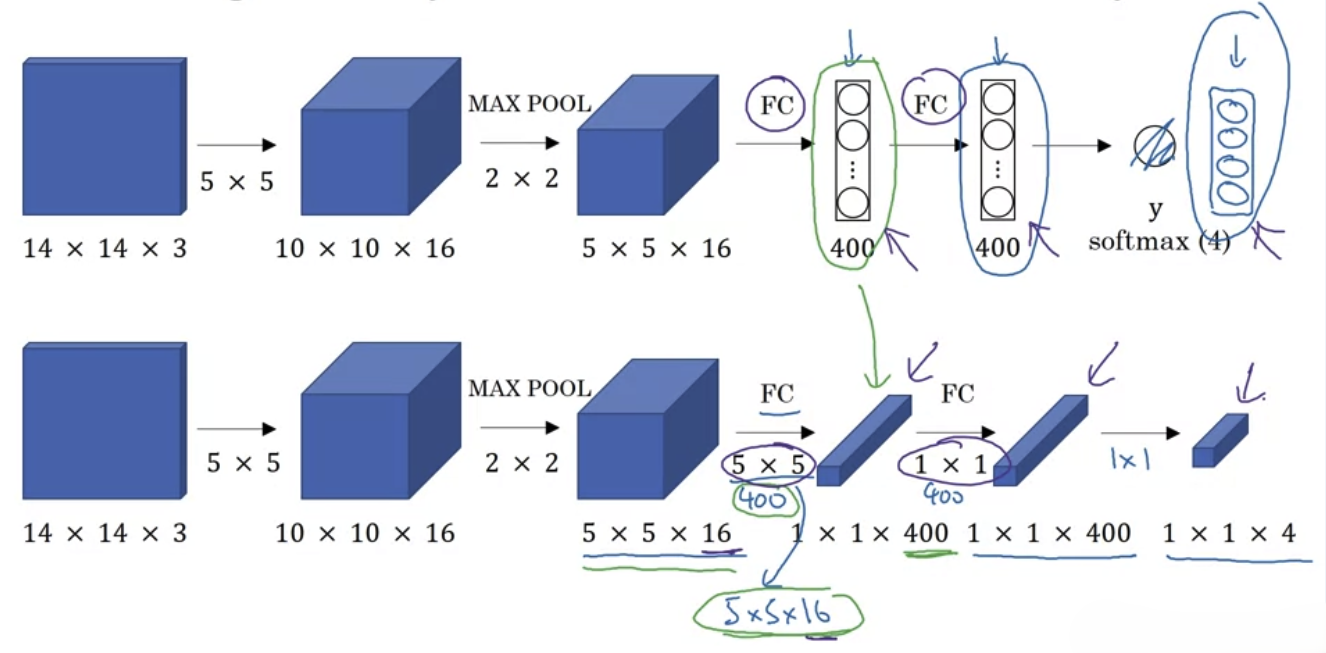
\includegraphics[width=0.85\textwidth]{Images/FC to Convolution.png}
	\caption{Converting Fully Connected Layers to Convolutional Layers}
	\label{fig:42}
\end{figure}
\FloatBarrier

\subsubsection*{Convolutional Implementation of Sliding Windows Detection}

Let us now see how this approach improves the Sliding Windows algorithm:
\begin{enumerate}
    \item Suppose your test image is $16 \times 16 \times 3$:
    \begin{itemize}
        \item In the standard Sliding Windows algorithm, you would crop regions of size $14 \times 14 \times 3$, process each through the ConvNet, and predict class labels.
        \item This requires running the ConvNet multiple times, once for each region, leading to redundant computations.
    \end{itemize}
    \item Instead, in the convolutional implementation:
    \begin{itemize}
        \item Pass the entire image ($16 \times 16 \times 3$) through the ConvNet in one forward pass.
        \item Perform convolutions with shared computations to generate a $2 \times 2 \times 4$ output volume, where each $1 \times 1 \times 4$ region corresponds to the prediction for a $14 \times 14$ patch of the input image.
        \item Each $1 \times 1 \times 4$ section in the output volume maps to a specific region of the input image (e.g., top-left, top-right, bottom-left, bottom-right).
    \end{itemize}
\end{enumerate}

The Advantages of the Convolutional Approach is:
\begin{itemize}
    \item \textbf{Efficiency:} By sharing computations across overlapping regions, the convolutional implementation significantly reduces the computational cost.
    \item \textbf{Scalability:} The approach works seamlessly for larger images. For example, processing a $28 \times 28 \times 3$ image results in an $8 \times 8 \times 4$ output volume, corresponding to predictions for each $14 \times 14$ region with a stride of 2.
\end{itemize}

While the convolutional implementation of Sliding Windows is more efficient, it still has one key limitation:
\begin{itemize}
    \item \textbf{Bounding Box Accuracy:} The positions of the bounding boxes may not be very accurate.
\end{itemize}

% ---------------- Bounding Box Predictions ----------------------%
\subsection{Improving Bounding Box Predictions: The YOLO Algorithm}
The YOLO (You Only Look Once) algorithm, addresses the limitations in producing accurate bounding boxes encountered by the convolutional implementation of Sliding Windows and provides more precise bounding box predictions.

YOLO, developed by Joseph Redmon, Santosh Divvala, Ross Girshick, and Ali Farhadi, transforms object detection into a regression problem that predicts bounding boxes and class probabilities directly from the image. 

\subsubsection*{Grid-Based Detection}
\begin{itemize}
    \item Divide the input image into a grid. For simplicity, consider a $3 \times 3$ grid (in practice, grids such as $19 \times 19$ are used for finer granularity).
    \item Each grid cell is responsible for detecting objects whose midpoint falls within that cell.
    \item For each grid cell, the algorithm predicts:
    \begin{itemize}
        \item $p_c$: Probability that an object exists in the grid cell.
        \item $b_x$, $b_y$, $b_h$, $b_w$: Bounding box parameters relative to the grid cell.
        \item $c_1$, $c_2$, $c_3$: Class probabilities (e.g., pedestrian, car, motorcycle).
    \end{itemize}
\end{itemize}

\subsubsection*{Target Label Representation}
\begin{itemize}
    \item For each grid cell, the label $y$ is an 8-dimensional vector:
    \[
    y = \begin{bmatrix}
    p_c & b_x & b_y & b_h & b_w & c_1 & c_2 & c_3
    \end{bmatrix}
    \]
    \item If no object exists in the grid cell, $p_c = 0$, and the remaining components are ``don't care.''
    \item For a grid cell with an object:
    \begin{itemize}
        \item $p_c = 1$.
        \item $b_x$, $b_y$: Coordinates of the object's midpoint, normalized to the grid cell.
        \item $b_h$, $b_w$: Height and width of the bounding box, normalized to the grid cell dimensions.
        \item $c_1, c_2, c_3$: Class labels as one-hot vectors.
    \end{itemize}
    \item The output for a $3 \times 3$ grid is a $3 \times 3 \times 8$ volume, where each $1 \times 1 \times 8$ vector corresponds to one grid cell.
\end{itemize}

\subsubsection*{Training the Neural Network}
\begin{itemize}
    \item The input to the network is an image (e.g., $100 \times 100 \times 3$).
    \item The network consists of convolutional layers, max-pooling layers, and fully connected layers, designed to map the input image to a $3 \times 3 \times 8$ output volume.
    \item During training:
    \begin{itemize}
        \item Use labeled data with input images and target labels $y$ (e.g., $3 \times 3 \times 8$).
        \item Train the network using backpropagation to minimize the loss between predicted and target outputs.
    \end{itemize}
\end{itemize}

The Advantages of YOLO algorithms is:
\begin{itemize}[nosep]
    \item \textbf{Precision:} Outputs bounding boxes with precise coordinates and aspect ratios.
    \item \textbf{Efficiency:} YOLO uses a convolutional implementation, sharing computation across grid cells, making it highly efficient for real-time detection.
    \item \textbf{Scalability:} Finer grids (e.g., $19 \times 19$) reduce the likelihood of multiple objects being assigned to the same grid cell.
\end{itemize}

\subsubsection*{Bounding Box Encoding}
\begin{itemize}
    \item Bounding box parameters ($b_x$, $b_y$, $b_h$, $b_w$) are defined relative to the grid cell:
    \begin{itemize}
        \item $(0, 0)$: Upper-left corner of the grid cell.
        \item $(1, 1)$: Lower-right corner of the grid cell.
    \end{itemize}
    \item For example, if the midpoint of a bounding box is at $(0.4, 0.3)$ within the grid cell, $b_x = 0.4$ and $b_y = 0.3$.
    \item $b_h$ and $b_w$ represent the height and width of the bounding box, normalized to the grid cell dimensions.
\end{itemize}

\subsubsection*{Challenges and Refinements}
\begin{itemize}
    \item Handling multiple objects within the same grid cell is a challenge addressed in later refinements.
    \item Advanced parametrizations (e.g., using sigmoid functions) ensure values like $b_x, b_y \in [0, 1]$ and $b_h, b_w \geq 0$ for improved stability.
\end{itemize}

The YOLO algorithm efficiently predicts bounding boxes and class probabilities for objects in an image, making it suitable for real-time object detection. While the algorithm has some complexities, its convolutional implementation and performance have made it a popular choice in computer vision. 

% ---------------- Intersection Over Union ----------------------%
\subsection*{Intersection Over Union (IoU)}

To evaluate the performance of an object detection algorithm, we use a metric called \textbf{Intersection Over Union (IoU)}. This metric helps to determine how well your algorithm localizes objects. IoU is used both for evaluation and as a component in improving the algorithm. Let us explore how it works.

\begin{itemize}
    \item In object detection, the goal is to localize objects by predicting bounding boxes.
    \item IoU measures the overlap between the \textit{predicted bounding box} and the \textit{ground-truth bounding box}.
    \item The \textbf{intersection} is the area of overlap between the predicted and ground-truth bounding boxes.
    \item The \textbf{union} is the total area covered by both the predicted and ground-truth bounding boxes.
    \item IoU is computed as:
    \[
    \text{IoU} = \frac{\text{Area of Intersection}}{\text{Area of Union}}
    \]
\end{itemize}

\subsubsection*{Interpreting IoU Values}
\begin{itemize}
    \item If the predicted and ground-truth bounding boxes overlap perfectly, IoU = 1.
    \item By convention, a predicted bounding box is considered \textit{correct} if:
    \[
    \text{IoU} \geq 0.5
    \]
    \item Thresholds can vary depending on the application:
    \begin{itemize}
        \item \textbf{More stringent criteria:} Use thresholds like 0.6 or 0.7 to demand higher accuracy.
        \item \textbf{Less stringent criteria:} Lower thresholds are rarely used (e.g., below 0.5).
    \end{itemize}
\end{itemize}

% ---------------- Non-Max Suppression ----------------------%
\subsection*{Non-Max Suppression}
One of the challenges in object detection is that an algorithm may detect the same object multiple times, resulting in overlapping bounding boxes. \textbf{Non-Max Suppression (NMS)} is a technique used to ensure that each object is detected only once. Let us go through an example and the steps of the algorithm.

\subsubsection*{Example of Non-Max Suppression}
\begin{itemize}[nosep]
    \item Suppose we want to detect pedestrians, cars, and motorcycles in an image.
    \item A grid (e.g., a $19 \times 19$ grid) is placed over the image, and an object classification and localization algorithm is run for every grid cell.
    \item It is common for multiple grid cells to predict the same object, resulting in overlapping bounding boxes.
    \item For instance, multiple grid cells might predict the presence of a car with different bounding boxes and probabilities.
\end{itemize}

% Figure 43
\begin{figure}[h]
	\centering
	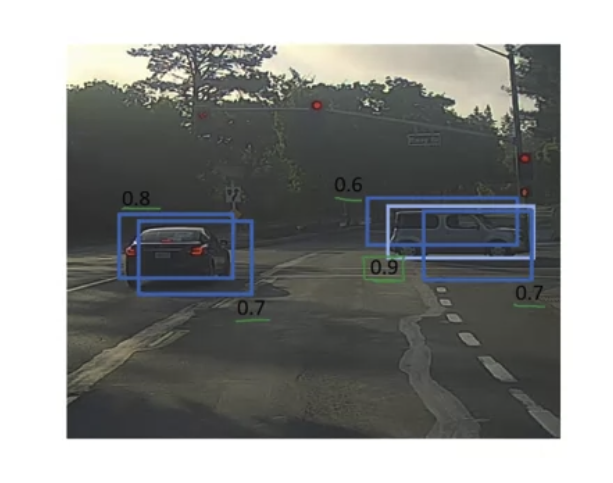
\includegraphics[width=0.75\textwidth]{Images/Non-Max Suppression Example.png}
	\caption{Example of Non-Max Suppression}
	\label{fig:43}
\end{figure}
\FloatBarrier

\subsubsection*{How Non-Max Suppression Works}
\begin{itemize}
    \item Non-Max Suppression eliminates redundant predictions and retains only the most confident ones.
    \item \textbf{Steps:}
    \begin{enumerate}
        \item Identify the bounding box with the highest confidence score ($p_c$).
        \item Commit to this bounding box as a prediction.
        \item Suppress all other bounding boxes that have a high overlap (\textbf{IoU}) with the selected bounding box.
        \item Repeat the process for the next highest confidence score until all boxes are processed.
    \end{enumerate}
    \item This ensures that only one bounding box per object is retained.
\end{itemize}

% Figure 44
\begin{figure}[h]
	\centering
	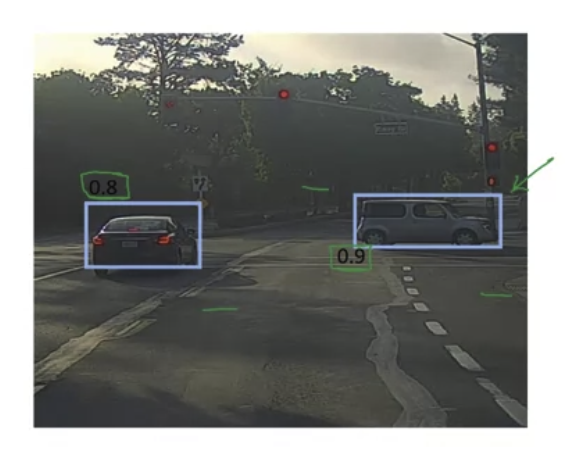
\includegraphics[width=0.75\textwidth]{Images/Non-Max Suppression Working.png}
	\caption{Non-Max Suppression}
	\label{fig:44}
\end{figure}
\FloatBarrier

\subsubsection*{Algorithm Steps}
\begin{enumerate}[nosep]
    \item Start with a $19 \times 19 \times 8$ output volume (e.g., for detecting a single object, this simplifies to $19 \times 19 \times 5$, which includes $p_c$ and bounding box parameters).
    \item \textbf{Step 1:} Discard all bounding boxes with $p_c \leq \text{threshold}$ (e.g., $p_c \leq 0.6$).
    \item \textbf{Step 2:} While there are remaining bounding boxes:
    \begin{itemize}
        \item Select the box with the highest $p_c$ and output it as a prediction.
        \item Suppress (discard) all other boxes with a high \textbf{IoU} with the selected box.
    \end{itemize}
    \item Repeat until all boxes are either processed or discarded.
\end{enumerate}

\subsubsection*{Multiple Object Classes}
\begin{itemize}[nosep]
    \item If detecting multiple classes (e.g., pedestrians, cars, and motorcycles), the algorithm needs to be run separately for each class.
    \item Perform Non-Max Suppression independently for each class' output vector.
    \item This ensures that predictions for different classes are handled correctly.
\end{itemize}

\subsubsection*{Benefits of Non-Max Suppression}
\begin{itemize}[nosep]
    \item Ensures that each object is detected only once.
    \item Reduces the number of redundant predictions.
    \item Improves the clarity and accuracy of object detection results.
\end{itemize}

% ---------------- Anchor boxes ----------------------%
\subsection*{Anchor Boxes}
Anchor boxes further improve the YOLO algorithm's ability to detect objects with varying shapes and sizes.
One of the limitations of object detection, as introduced so far, is that each grid cell can detect only one object. However, what happens if multiple objects share the same grid cell? \textbf{Anchor Boxes} provide a solution by enabling multiple detections per grid cell.

Consider a $3 \times 3$ grid over an image containing a pedestrian and a car.
\begin{itemize}[nosep]
    \item The midpoints of both objects may fall into the same grid cell.
    \item Without anchor boxes, the grid cell can only detect one object, requiring a choice between the pedestrian or the car.
    \item \textbf{Anchor Boxes:} Pre-define shapes called \textit{anchor boxes}, allowing each grid cell to associate multiple predictions with multiple anchor boxes.
\end{itemize}

\subsubsection*{Structure of the Output Vector}
\begin{itemize}
    \item Instead of a single output vector, each grid cell now predicts multiple vectors, one for each anchor box.
    \item For two anchor boxes:
    \[
    Y = \big[\text{Anchor Box 1: } p_c, b_x, b_y, b_h, b_w, c_1, c_2, c_3; \text{Anchor Box 2: } p_c, b_x, b_y, b_h, b_w, c_1, c_2, c_3\big]
    \]
    \item For $k$ anchor boxes, the output becomes $3 \times 3 \times k \times 8$, where $8$ represents the number of parameters (e.g., $p_c$, bounding box, class probabilities).
\end{itemize}

\subsubsection*{Assignment of Objects to Anchor Boxes}
\begin{itemize}
    \item Each object is assigned to the grid cell containing its midpoint, as before.
    \item Additionally, the object is assigned to the anchor box with the highest \textbf{Intersection over Union (IoU)} with its bounding box.
    \item Example:
    \begin{itemize}
        \item If the pedestrian's bounding box matches Anchor Box 1, it is assigned to that anchor box.
        \item If the car's bounding box matches Anchor Box 2, it is assigned to that anchor box.
    \end{itemize}
\end{itemize}

\subsubsection*{Output Dimensions}
\begin{itemize}
    \item Without anchor boxes, $Y$ is $3 \times 3 \times 8$.
    \item With two anchor boxes, $Y$ becomes $3 \times 3 \times 16$, or equivalently $3 \times 3 \times 2 \times 8$.
    \item For a $19 \times 19$ grid with $k$ anchor boxes, $Y$ becomes $19 \times 19 \times k \times 8$.
\end{itemize}

\subsubsection*{Handling Special Cases}
\begin{itemize}
    \item \textbf{Two Objects with the Same Anchor Box:} If two objects in the same grid cell are assigned to the same anchor box, a tie-breaking rule is needed.
    \item \textbf{Three Objects in One Grid Cell:} If more objects exist than anchor boxes, a tie-breaking mechanism must be applied.
\end{itemize}

\subsubsection*{Advantages of Anchor Boxes}
\begin{itemize}
    \item \textbf{Supports Multiple Detections:} Allows each grid cell to detect multiple objects.
    \item \textbf{Specialization:} Anchor boxes enable the network to specialize in detecting objects of different shapes and sizes (e.g., tall, skinny pedestrians vs. wide, fat cars).
\end{itemize}

\subsubsection*{Choosing Anchor Boxes}
There are several ways to choose Anchor boxes. They include:
\begin{itemize}
    \item \textbf{Manual Selection:} Choose shapes that span a variety of object sizes (e.g., tall, skinny, wide, fat).
    \item \textbf{K-Means Clustering:} A more advanced method is to use K-means clustering to group object shapes in the dataset and determine anchor boxes representative of these clusters.
\end{itemize}

In Summary:
\begin{itemize}[nosep]
    \item Anchor boxes allow each grid cell to detect multiple objects by associating objects with anchor boxes based on IoU.
    \item This results in more flexible and accurate object detection.
    \item In the next section, these concepts will be tied back to the YOLO algorithm for efficient object detection.
\end{itemize}


% ---------------- YOLO Algorithm ----------------------%
\subsection{YOLO Object Detection Algorithm}
The YOLO (\textbf{You Only Look Once}) object detection algorithm integrates many key components of object detection into a unified framework. This section outlines the process of training, prediction, and post-processing for YOLO.

\subsubsection*{Training the Neural Network}

\paragraph{Training Set Construction:}
\begin{itemize}
    \item Suppose you are detecting three classes: \textbf{pedestrians}, \textbf{cars}, and \textbf{motorcycles}.
    \item You also include the \textbf{background class}.
    \item Using a $3 \times 3$ grid and $2$ anchor boxes, the output $y$ for each grid cell is $3 \times 3 \times 2 \times 8$, where:
    \begin{itemize}
        \item $8 = 5 + 3$: 
        \begin{itemize}
            \item $5$ consists of $p_c$, $b_x$, $b_y$, $b_h$, and $b_w$ (confidence and bounding box parameters).
            \item $3$ corresponds to the class probabilities $c_1$, $c_2$, and $c_3$.
        \end{itemize}
        \item Alternatively, $y$ can be viewed as $3 \times 3 \times 16$ (flattened representation).
    \end{itemize}
\end{itemize}

\paragraph{Label Encoding:}
\begin{itemize}
    \item For each grid cell:
    \begin{itemize}
        \item If no object exists in the cell, $p_c = 0$ and the rest of the vector contains ``don't care'' values.
        \item If an object exists:
        \begin{itemize}
            \item Assign the object to the anchor box with the highest \textbf{IoU} (Intersection over Union).
            \item Encode the bounding box parameters and class label in the corresponding anchor box vector.
        \end{itemize}
    \end{itemize}
    \item Example:
    \begin{itemize}
        \item For a car with a bounding box aligned to \textbf{Anchor Box 2}, $p_c = 1$, the bounding box parameters are encoded, and $c_2 = 1$ (car class).
    \end{itemize}
\end{itemize}

\paragraph{Final Output Volume:}
\begin{itemize}
    \item For a $3 \times 3$ grid with $2$ anchor boxes, the output volume is $3 \times 3 \times 16$.
    \item In practice, larger grids (e.g., $19 \times 19$) and more anchor boxes (e.g., $5$) are used:
    \[
    y = 19 \times 19 \times 40 \quad \text{(if using 5 anchor boxes and 3 classes)}.
    \]
\end{itemize}

\subsubsection*{Making Predictions}

\paragraph{Neural Network Output:}
\begin{itemize}
    \item Input image: $100 \times 100 \times 3$.
    \item Output volume: $3 \times 3 \times 16$ (or more in practice).
    \item For each grid cell:
    \begin{itemize}
        \item If $p_c = 0$, the other values are ignored as noise.
        \item If $p_c = 1$, the bounding box parameters and class probabilities specify the detection.
    \end{itemize}
\end{itemize}

\subsubsection*{Post-Processing: Non-Max Suppression}
\paragraph{Steps:}
\begin{enumerate}[nosep]
    \item For each grid cell, two bounding boxes (for two anchor boxes) are predicted.
    \item Discard predictions with low probabilities ($p_c \leq 0.6$).
    \item For each class (\textbf{pedestrians}, \textbf{cars}, \textbf{motorcycles}):
    \begin{itemize}
        \item Apply \textbf{non-max suppression} to remove duplicate detections of the same object.
    \end{itemize}
    \item Final output: One bounding box per detected object.
\end{enumerate}

In Summary:
\begin{itemize}[nosep]
    \item The YOLO algorithm is one of the most effective object detection methods.
    \item You train a ConvNet to predict bounding boxes and class probabilities for each grid cell and anchor box.
    \item Post-processing with non-max suppression refines the predictions to ensure accurate detections.
\end{itemize}

% ---------------- Semantic Segmentation with U-Net ----------------------%
\subsection{Semantic Segmentation with U-Net}
In this section, we explore \textbf{semantic segmentation}, an advanced computer vision technique that goes beyond object recognition and object detection. The goal of semantic segmentation is to assign a class label to every pixel in an image, thereby outlining objects with pixel-level precision.

% Figure 45
\begin{figure}[h]
	\centering
	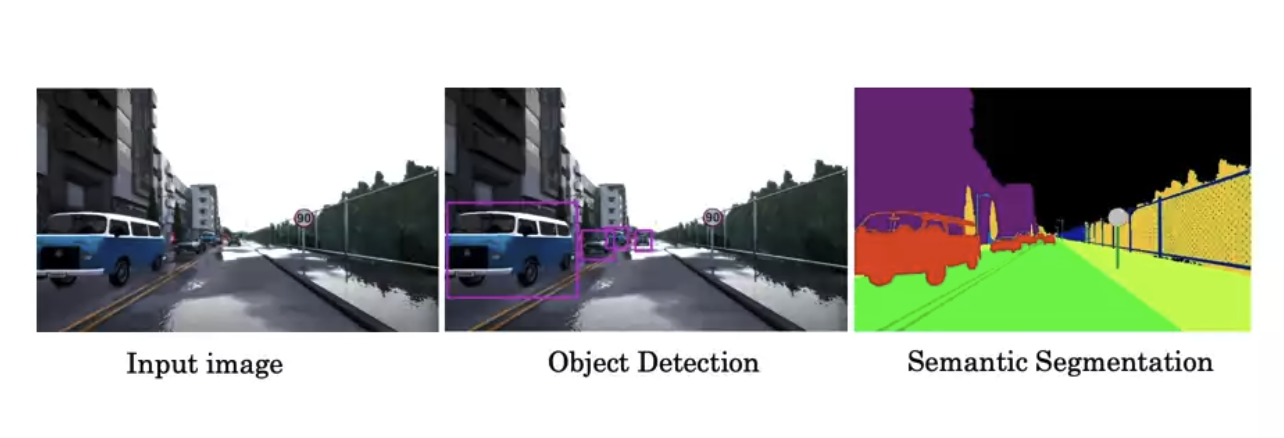
\includegraphics[width=\textwidth]{Images/Object Detection vs Semantic Segmentation.png}
	\caption{Object Detection vs Semantic Segmentation}
	\label{fig:45}
\end{figure}
\FloatBarrier

\paragraph{Definition:} Semantic segmentation involves labeling every pixel in an image with its corresponding class. Semantic Segmentation finds application in:
\begin{itemize}
    \item \textbf{Autonomous Vehicles:} Detecting drivable roads, vehicles, and pedestrians with pixel-level accuracy.
    \item \textbf{Medical Imaging:} 
    \begin{itemize}
        \item Segmenting lungs, heart, and clavicles from chest X-rays for diagnostic purposes.
        \item Automatically identifying brain tumors in MRI scans to assist radiologists and surgeons.
    \end{itemize}
\end{itemize}

\subsubsection*{Per-Pixel Classification:}
Imagine we are segmenting out a car from some background. Let's say for now that the only thing you care about is segmenting out the car in this image. In that case, you may decide to have two class labels. One for a car and zero for not car. 

\begin{itemize}
    \item Each pixel is assigned a label:
    \begin{itemize}
        \item Example: $1$ for car pixels, $0$ for non-car pixels.
        \item Alternatively, multiple classes can be defined:
        \begin{itemize}
            \item Class $1$: Car
            \item Class $2$: Building
            \item Class $3$: Ground/Road
        \end{itemize}
    \end{itemize}
\end{itemize}

\paragraph{Output:}
\begin{itemize}
    \item Instead of outputting a single class label or bounding box, the network generates a \textbf{segmentation map}, a matrix where each element corresponds to the class label of a pixel.
\end{itemize}

% Figure 46
\begin{figure}[h]
	\centering
	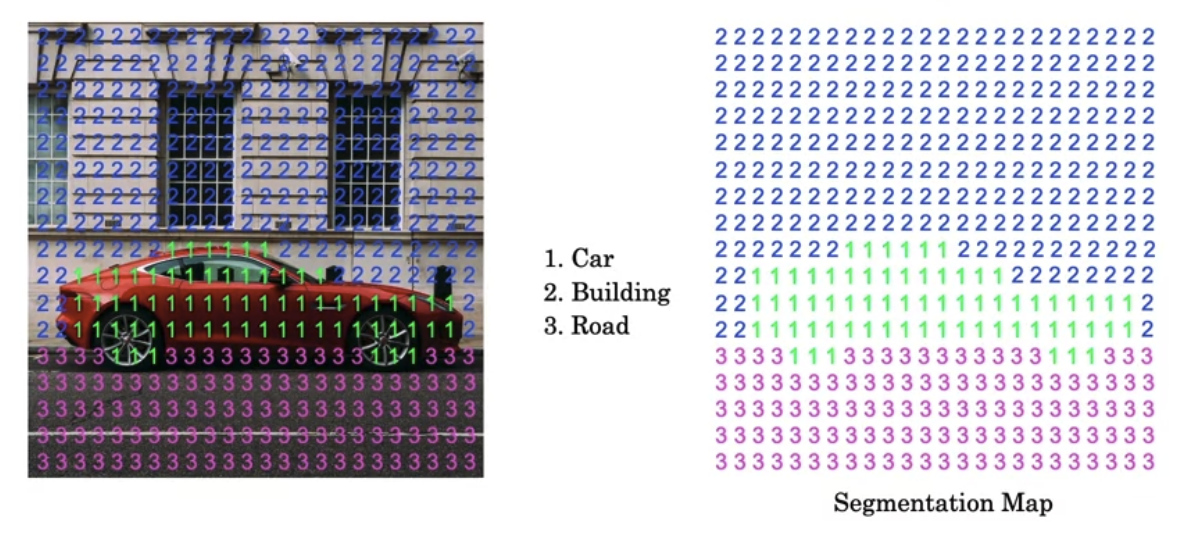
\includegraphics[width=\textwidth]{Images/Segmentation Map.png}
	\caption{Per-pixel class labels on a segmentation map}
	\label{fig:46}
\end{figure}
\FloatBarrier

\paragraph{U-Net Architecture:}
\begin{itemize}
    \item \textbf{Encoder:} Reduces the spatial dimensions while increasing the number of channels.
    \item \textbf{Decoder:} Gradually increases the spatial dimensions to match the original image size while reducing the number of channels.
    \item The architecture forms a ``U'' shape, hence the name \textbf{U-Net}.
\end{itemize}

\paragraph{Key Operation in the U-Net Architecture: Transpose Convolution}
\begin{itemize}
    \item Used to ``blow up'' small sets of activations to match the original image size.
    \item Essential for generating full-size segmentation maps in the decoder phase of U-Net.
\end{itemize}

Semantic segmentation is a powerful tool in computer vision, enabling pixel-level classification for applications such as autonomous driving and medical imaging. The key idea is to use a network like \textbf{U-Net}, which combines encoding and decoding stages to produce a segmentation map. The next step in understanding this architecture is to learn about \textbf{transpose convolutions}, an essential operation in the decoder. 

% ---------------- Transpose Convolutions ----------------------%
\subsubsection*{Transpose Convolutions}
The \textbf{transpose convolution} is a critical operation used in the U-Net architecture for semantic segmentation. It allows you to take smaller input dimensions and ``blow them up'' into larger output dimensions, effectively reversing the dimensionality reduction performed by regular convolutions.

\paragraph{Purpose:} A transpose convolution enables you to expand the spatial dimensions of the input while maintaining the learned relationships through filters. For example:
\begin{itemize}
    \item Input: $2 \times 2$
    \item Output: $4 \times 4$
\end{itemize}

\paragraph{Comparison with Regular Convolution:}
\begin{itemize}
    \item Regular convolution reduces spatial dimensions.
    \item Transpose convolution increases spatial dimensions.
\end{itemize}

\subsubsection*{Details of Transpose Convolution}
\paragraph{Example Setup:} Consider a $2 \times 2$ input and the goal is to obtain a $4 \times 4$ output. Parameters:
\begin{itemize}[nosep]
    \item \textbf{Filter size:} $3 \times 3$
    \item \textbf{Padding:} $p = 1$
    \item \textbf{Stride:} $s = 2$
\end{itemize}

\paragraph{Steps:}
\begin{enumerate}
    \item \textbf{For each input value:}
    \begin{itemize}
        \item Multiply the input value by each element of the filter.
        \item Copy the resulting $3 \times 3$ values into the corresponding positions of the output matrix.
    \end{itemize}
    \item \textbf{Handle overlaps:}
    \begin{itemize}
        \item Where multiple filters contribute to the same output position, their values are summed.
    \end{itemize}
    \item \textbf{Padding and stride:}
    \begin{itemize}
        \item Padding determines how much ``empty space'' surrounds the input.
        \item Stride determines the step size for positioning the filter over the output matrix.
    \end{itemize}
\end{enumerate}

\subsubsection*{Illustrative Example}

\paragraph{Setup:} 
\begin{itemize}[nosep]
    \item Input: $2 \times 2$
    \item Filter: $3 \times 3$
    \item Padding: $p = 1$
    \item Stride: $s = 2$
\end{itemize}

\paragraph{Step-by-Step Process:}
\begin{enumerate}
    \item \textbf{Input value: $2$ (top-left corner):}
    \begin{itemize}
        \item Multiply the filter by $2$ and copy the $3 \times 3$ values to the corresponding output positions.
    \end{itemize}
	% Figure 47
	\begin{figure}[h]
		\centering
		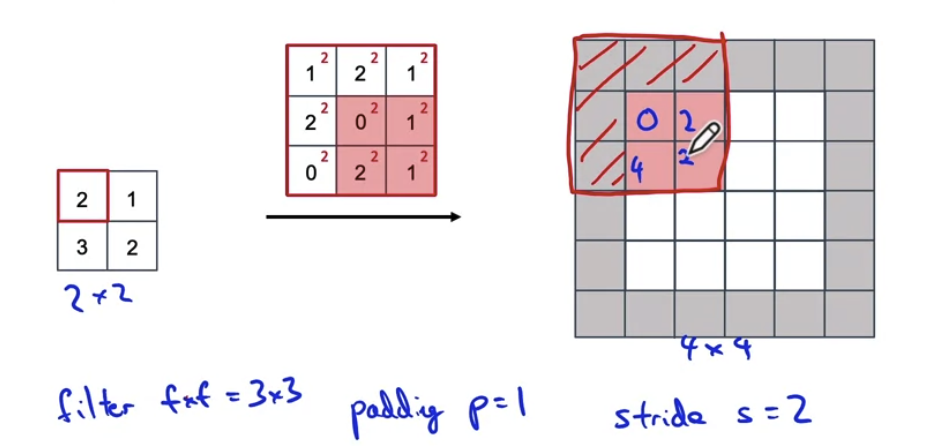
\includegraphics[width=0.85\textwidth]{Images/Transpose Convolution - Step 1.png}
		\label{fig:47}
	\end{figure}
	\FloatBarrier

    \item \textbf{Input value: $1$ (top-right corner):}
    \begin{itemize}
        \item Multiply the filter by $1$ and shift the copied values by two steps (stride of 2).
    \end{itemize}
	% Figure 48
	\begin{figure}[h]
		\centering
		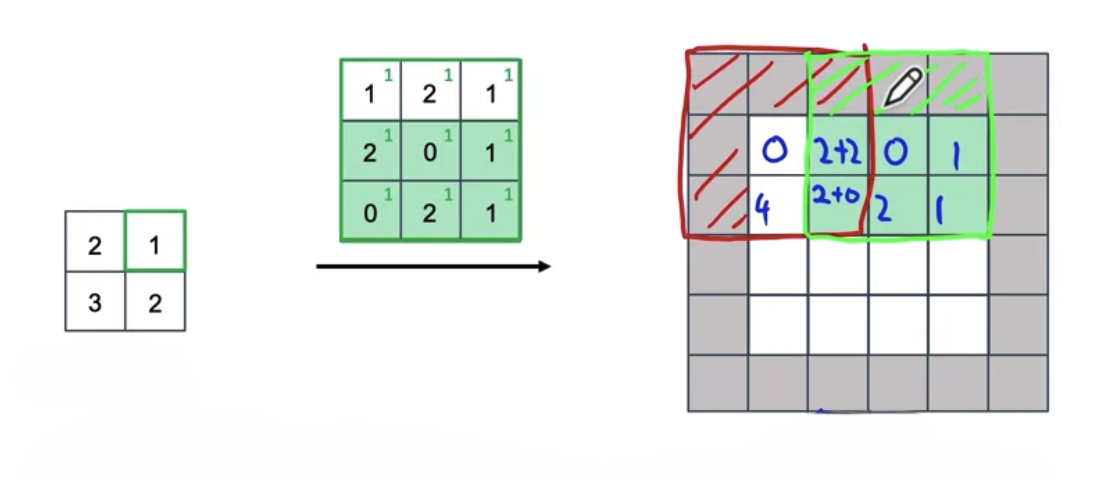
\includegraphics[width=0.85\textwidth]{Images/Transpose Convolution - Step 2.png}
		\label{fig:48}
	\end{figure}
	\FloatBarrier

    \item \textbf{Input value: $3$ (bottom-left corner):}
    \begin{itemize}
        \item Multiply the filter by $3$ and copy values into the next block of the output matrix.
    \end{itemize}
	% Figure 49
	\begin{figure}[h]
		\centering
		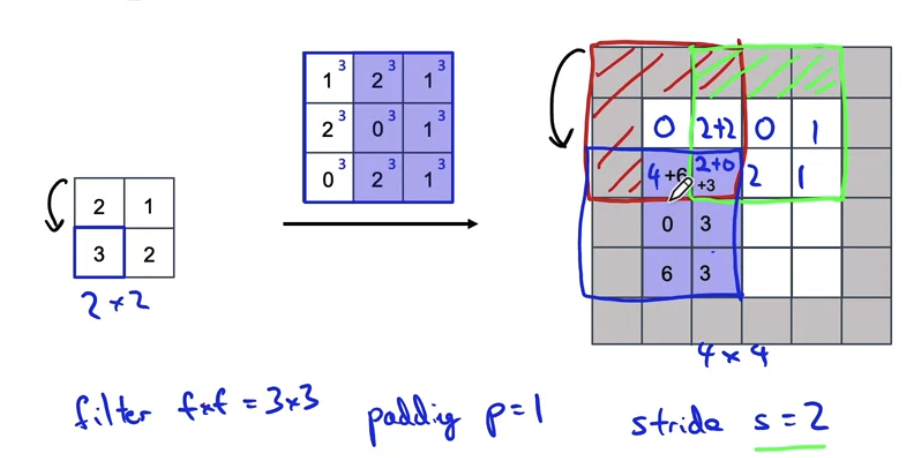
\includegraphics[width=0.85\textwidth]{Images/Transpose Convolution - Step 3.png}
		\label{fig:49}
	\end{figure}
	\FloatBarrier

    \item \textbf{Input value: $2$ (bottom-right corner):}
    \begin{itemize}
        \item Multiply the filter by $2$ and copy values into the final block.
    \end{itemize}

	% Figure 50
	\begin{figure}[h]
		\centering
		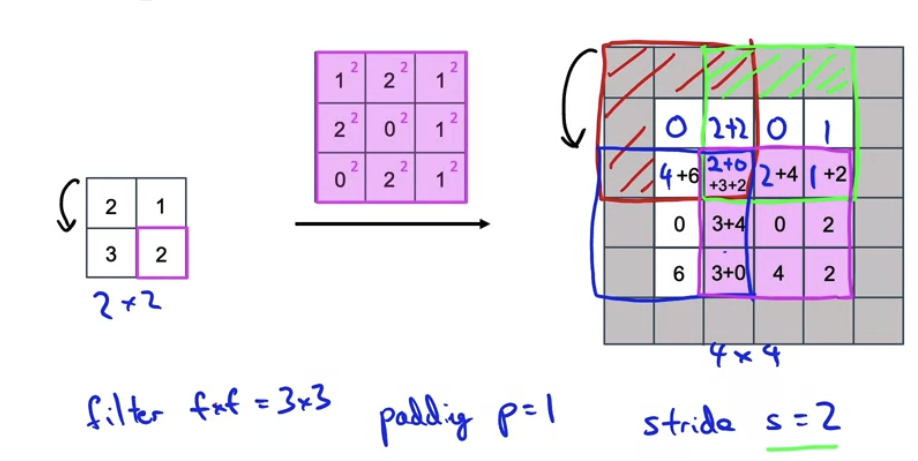
\includegraphics[width=0.85\textwidth]{Images/Transpose Convolution - Step 4.png}
		\label{fig:50}
	\end{figure}
	\FloatBarrier

    \item \textbf{Combine overlapping regions:}
    \begin{itemize}
        \item Sum the values where the contributions from multiple filters overlap.
    \end{itemize}
	% Figure 51
	\begin{figure}[h]
		\centering
		\includegraphics[width=0.85\textwidth]{Images/Transpose Convolution - Final Step.png}
		\label{fig:51}
	\end{figure}
	\FloatBarrier
\end{enumerate}

\paragraph{Final Output:} The resulting $4 \times 4$ matrix contains the summed contributions from all input values and their corresponding filter multiplications.

The key insights is:
\begin{itemize}[nosep]
    \item \textbf{Flexibility:} The transpose convolution allows for controlled expansion of spatial dimensions.
    \item \textbf{Learning:} The filter parameters are learned during training, enabling the network to effectively ``blow up'' activations in a meaningful way.
    \item \textbf{Applications:} Transpose convolutions are a key building block of the U-Net architecture used for semantic segmentation.
\end{itemize}

The transpose convolution is essential for increasing spatial dimensions in networks like U-Net. By understanding how it works step by step, you can effectively implement and use it in semantic segmentation tasks. 

% ---------------- U-Net Architecture Intuition ----------------------%
\subsection{U-Net Architecture Intuition}
The U-Net is a neural network architecture specifically designed for \textbf{semantic segmentation}. It processes an image through two main stages:
\begin{itemize}
    \item \textbf{Compression:} Reduces the spatial dimensions while capturing high-level contextual information.
    \item \textbf{Expansion:} Increases the spatial dimensions back to the original size for pixel-wise predictions.
\end{itemize}

\paragraph{Key Features:}
\begin{itemize}
    \item Uses regular convolutions for the compression stage.
    \item Uses transpose convolutions for the expansion stage.
    \item Incorporates \textbf{skip connections} to enhance performance by combining high-resolution, low-level features with low-resolution, high-level contextual information.
\end{itemize}

\subsubsection*{Compression Stage}

The first half of the U-Net architecture:
\begin{itemize}
    \item \textbf{Purpose:} Reduces the spatial dimensions (height and width) of the input image.
    \item \textbf{Effect:} Compresses spatial information while increasing the depth (number of channels).
    \item \textbf{Outcome:} Captures high-level contextual information but loses fine-grained spatial details.
\end{itemize}

For example:
\begin{itemize}
    \item The middle layer might represent a general understanding that there is a cat in the lower right-hand corner of the image.
    \item However, the precise spatial details (e.g., the exact shape or boundaries of the cat) are lost due to the reduced resolution.
\end{itemize}

\subsubsection*{Expansion Stage}

The second half of the U-Net architecture:
\begin{itemize}
    \item \textbf{Purpose:} Expands the spatial dimensions back to the size of the original input image.
    \item \textbf{Method:} Uses \textbf{transpose convolutions} to achieve this expansion.
    \item \textbf{Outcome:} Produces an output with the same resolution as the input image, allowing for pixel-wise predictions.
\end{itemize}

\subsubsection*{Skip Connections}

To improve the performance of the U-Net, \textbf{skip connections} are added between the compression and expansion stages:
\begin{itemize}
    \item \textbf{Mechanism:} Connect earlier layers (from the compression stage) directly to later layers (in the expansion stage).
    \item \textbf{Purpose:} Provides the network with detailed, high-resolution, low-level feature information.
\end{itemize}

\paragraph{Why Skip Connections Are Useful:}
\begin{itemize}
    \item The expansion layers rely on low-resolution, high-level contextual information from the compression stage to make predictions.
    \item However, this information alone is insufficient for precise pixel-wise classification.
    \item Skip connections allow the network to access:
    \begin{itemize}
        \item High-level contextual information (from compressed activations).
        \item Fine-grained, high-resolution spatial information (from earlier layers).
    \end{itemize}
\end{itemize}

\paragraph{Example:}
For a layer making the decision about whether a pixel belongs to a cat:
\begin{itemize}
    \item The compressed activations may provide high-level information (e.g., the general location of the cat in the image).
    \item The skip connections provide detailed, low-level information (e.g., texture or fur patterns at specific pixel positions).
\end{itemize}

By combining these two types of information, the network can make more accurate predictions for semantic segmentation.

% ---------------- U-Net Architecture: Detailed Explanation ----------------------%
\subsection*{U-Net Architecture: Detailed Explanation}
The U-Net architecture is one of the foundational neural network architectures in computer vision, particularly for semantic segmentation. Initially developed by Olaf Ronneberger, Philipp Fischer, and Thomas Brox for biomedical image segmentation, it has since found applications in many other areas of computer vision. Below, we break down the U-Net architecture step-by-step.

\subsubsection*{Overview of the U-Net Architecture}

\begin{itemize}
    \item \textbf{Input:} An image of dimensions \( h \times w \times 3 \), where the three channels represent the RGB components.
    \item \textbf{Output:} A segmentation map of dimensions \( h \times w \times n_{classes} \), where each pixel is classified into one of the possible classes.
    \item \textbf{Key Feature:} Skip connections that transfer detailed spatial information from earlier layers to later layers during the up-sampling process.
\end{itemize}

The architecture has a U-shaped structure, hence the name ``U-Net.''

\subsubsection*{Compression Stage (Downsampling)}

The first half of the U-Net involves progressively reducing the spatial dimensions while increasing the depth (number of channels):
\begin{enumerate}
    \item \textbf{Convolutional Layers:} Each step involves a convolutional layer followed by a ReLU activation function.
    \item \textbf{Max Pooling:} After a couple of convolutional layers, max pooling is applied to reduce the spatial dimensions. This operation decreases the height and width while increasing the number of channels.
    \item This process is repeated several times, resulting in smaller spatial dimensions and deeper feature representations.
\end{enumerate}

\subsubsection*{Expansion Stage (Upsampling)}

The second half of the U-Net involves increasing the spatial dimensions back to the original size:
\begin{enumerate}
    \item \textbf{Transpose Convolutions:} Used to upsample the feature maps. This increases the height and width of the activations while reducing the depth.
    \item \textbf{Skip Connections:} 
    \begin{itemize}
        \item Feature maps from the corresponding layers in the compression stage are directly copied and concatenated with the upsampled activations.
        \item This provides fine-grained, high-resolution information to the later layers.
    \end{itemize}
    \item \textbf{Convolutional Layers:} After concatenation, more convolutional layers are applied to refine the activations.
    \item This process is repeated until the spatial dimensions are restored to match the input image.
\end{enumerate}

\subsubsection*{Final Output Layer}

\begin{itemize}
    \item After the last upsampling step, a \( 1 \times 1 \) convolution is applied to map the activations to the required number of classes ($n_{classes}$).
    \item The final output has dimensions \( h \times w \times n_{classes} \), where:
    \begin{itemize}
        \item \( h \) and \( w \): Height and width of the original input image.
        \item $n_{classes}$: Number of classes for segmentation.
    \end{itemize}
    \item \textbf{Pixel Classification:} For each pixel, the network outputs a vector of probabilities (one per class). Taking the \texttt{argmax} over this vector yields the final class label for each pixel.
\end{itemize}

\subsubsection*{Example Dimensions Throughout the U-Net}

\begin{enumerate}
    \item \textbf{Input:} \( h \times w \times 3 \) (e.g., \( 256 \times 256 \times 3 \)).
    \item \textbf{Compression Stage:} Gradually decreases to smaller dimensions like \( h/2 \times w/2 \times \text{more\_channels} \), \( h/4 \times w/4 \times \text{even\_more\_channels} \), and so on.
    \item \textbf{Expansion Stage:} Gradually increases back to \( h \times w \times \text{fewer\_channels} \).
    \item \textbf{Output:} \( h \times w \times n_{classes} \).
\end{enumerate}

\subsubsection*{Intuition Behind Skip Connections}

\begin{itemize}
    \item \textbf{High-Level Context:} The compressed activations provide high-level contextual information, e.g., ``a cat exists in the lower-right corner.''
    \item \textbf{Fine-Grained Details:} The skip connections pass detailed spatial features, e.g., ``this pixel is part of the cat's fur,'' from the early layers to the later layers.
    \item Combining these two types of information improves the segmentation accuracy.
\end{itemize}

The U-Net is a powerful architecture for semantic segmentation, combining high-level contextual understanding with fine-grained spatial details. Through its U-shaped design and skip connections, it achieves high accuracy across a variety of applications. You have now learned how the U-Net works, step-by-step, and can begin exploring its implementation in practice.

% Figure 52
\begin{figure}[h]
	\centering
	\includegraphics[width=\textwidth]{Images/U-Net.png}
	\caption{U-Net Architecture}
	\label{fig:52}
\end{figure}
\FloatBarrier

\end{document}

